\pdfoptionpdfminorversion=5
\documentclass[a4paper,11pt]{book}

\usepackage{amsmath, amssymb, amsthm}
\usepackage{xspace}
\usepackage{graphicx}
\usepackage{rotating}
\usepackage{multirow}
\usepackage{booktabs}
\usepackage{pbox}

\usepackage[bindingoffset=1cm,margin=2.5cm]{geometry}

\usepackage{cite}

\usepackage{tikz}

\usepackage[linktoc=all,
            colorlinks=true,
            linkcolor=black,citecolor=black,filecolor=black,urlcolor=black]{hyperref}

% Title Page
\title{\Huge The Razor Boost analysis\\[1cm]
Another step in the hunt for new physics at CMS \\[0.5cm] \textcolor{red}{(Preliminary title)}}
\author{Nadja Strobbe}


% short cuts
% particles
\newcommand{\W}{\ensuremath{W}}
\newcommand{\Pp}{\ensuremath{{p}}}
\newcommand{\Pap}{\ensuremath{{\overline{p}}}}
\newcommand{\cPZ}{\ensuremath{\mathrm{Z}}}
\newcommand{\cPqb}{\ensuremath{\mathrm{b}}}
\newcommand{\stopone}{\ensuremath{\tilde{t}_1}}
\newcommand{\stoptwo}{\ensuremath{\tilde{t}_2}}
\newcommand{\lsp}{\ensuremath{\tilde{\chi}_1^0}}

% units
\newcommand{\ten}[1]{\ensuremath{\times \text{10}^\text{#1}}}
\newcommand{\unit}[1]{\ensuremath{\text{\,#1}}\xspace}
\newcommand{\MeV}{\ensuremath{\,\text{Me\hspace{-.08em}V}}\xspace}
\newcommand{\GeV}{\ensuremath{\,\text{Ge\hspace{-.08em}V}}\xspace}
\newcommand{\TeV}{\ensuremath{\,\text{Te\hspace{-.08em}V}}\xspace}
\newcommand{\fbinv} {\mbox{\ensuremath{\,\text{fb}^\text{$-$1}}}\xspace}
\newcommand{\cm}{\ensuremath{\,\text{cm}}\xspace}
\newcommand{\mum}{\ensuremath{\,\mu\text{m}}\xspace}
\newcommand{\mus}{\ensuremath{\,\mu\text{s}}\xspace}
\newcommand{\second}{\ensuremath{\,\text{s}}\xspace}
\newcommand{\mm}{\ensuremath{\,\text{mm}}\xspace}
\newcommand{\meter}{\ensuremath{\,\text{m}}\xspace}
\newcommand{\de}{\ensuremath{^\circ}}
\newcommand{\percms}{\ensuremath{\,\text{cm}^\text{$-$2}\,\text{s}^\text{$-$1}}\xspace}

% programs
\newcommand{\MADGRAPH} {\textsc{MadGraph}\xspace}
\newcommand{\PYTHIA} {{\textsc{pythia}}\xspace}
\newcommand{\GEANTfour} {{\textsc{Geant4}}\xspace}
\newcommand{\POWHEG} {{\textsc{powheg}}\xspace}
\newcommand{\HERWIG} {{\textsc{herwig}}\xspace}
\newcommand{\AMCATNLO} {\textsc{aMC@NLO}\xspace}

% variables
\newcommand{\mr}{\ensuremath{\mathrm{M_R}}\xspace}
\newcommand{\mtr}{\ensuremath{\mathrm{M_T^R}}\xspace}
\newcommand{\rsq}{\ensuremath{\mathrm{R^2}}\xspace}
\newcommand{\betaCM}{\ensuremath{\vec{\beta}^{\,\textrm{CM}}}}

\newcommand{\ETm}{\ensuremath{E_{\mathrm{T}}^{\text{miss}}}\xspace}
\newcommand{\VEtmiss}{\ensuremath{{\vec E}_{\mathrm{T}}^{\text{miss}}}\xspace}
\newcommand{\pt}{\ensuremath{p_{\mathrm{T}}}\xspace}
\newcommand{\ET}{\ensuremath{E_{\mathrm{T}}}\xspace}
\newcommand{\HT}{\ensuremath{H_{\mathrm{T}}}
\xspace}
\newcommand{\ptvec}{\ensuremath{{\vec p}_{\mathrm{T}}}\xspace}
\newcommand{\mT}{\ensuremath{m_{\mathrm{T}}}\xspace}

% "theorems"
\theoremstyle{definition}
\newtheorem*{cajet}{Cambridge-Aachen jet algorithm}
%\theoremstyle{definition}

\begin{document}
\maketitle
% 
% \begin{abstract}
% \end{abstract}

\chapter*{Acknowledgements \label{sec:acknowledgements}}

...

\tableofcontents

\chapter{Introduction \label{chap:introduction}}

\textit{Curiosity.} Among all human traits, curiosity is the one that really drives progress and
innovation. Every child is born with it. It expresses itself as the relentless desire to learn about
the world, be it by eating dirt because you wondered what it tastes like, or by going through your
parents' cupboards even though that was not allowed. I am sure you can think of many more of these
examples. 
To me, this fundamental human trait is what science is all about. 

For centuries, scientists have investigated the world around them, pushing the boundaries of
our knowledge and coming to an ever better understanding of nature.
This exploration lead us to the biggest structures in the universe, the stars and galaxies, but
also to the smallest. First, atoms were discovered, thought at the time to be indivisible.
When Rutherford and Thomson showed that these atoms actually consist of a positive nucleus
surrounded by negative charges, that was a paradigm-shifting relevation. 

From then onward, theory and experiment worked hand-in-hand to come to the Standard Model of
particle physics. Many new particles were discovered during the past one hundred years or so. 
The electron, proton and neutron were the first to be discovered. Then a range of particles,
among which are the positron, pion and kaon, were identified in the study of cosmic rays. 
With the advent of particle accelerators, physicists were able to create and identify many more
particles. There were so many new particles in fact, without any apparent structure to them, that
they were called the `particle zoo'. Only when Gell-Mann and Zweig proposed that these particles
were composed of quarks, did pieces start falling into place. Experimental evidence of quarks was
found not much later. 

During the 1960s and 1970s, the theoretical formulation of the Standard Model took shape. 
The Standard Model describes the elementary particles and their interactions. In those days,
physicists already knew of all particles belonging to the first two families: the electron and
electron neutrino, the muon and muon neutrino, the up and down quarks, and the charm and strange
quarks. The tau lepton and bottom quark were discovered in the second half of the 1970s, indicating
the existance of a third family as well. If this family was to fit in the existing structure, two
more particles needed to exist: the tau neutrino, and the top quark. 
The Standard Model also predicted the existance of force carriers, in particular the gluon, and
the $\W$, $\cPZ$ and Higgs bosons. 
If the Standard Model was really to describe nature, then these particles needed to exist. And so
the hunt for these new particles began.

The gluon was discovered indirectly in 1979 at DESY, and the $\W$ and $\cPZ$ bosons were observed
in 1983 at CERN. The top quark was more difficult to find, it took until 1995 at Fermilab. The tau
neutrino was observed directly for the first time in 2000, also at Fermilab. The only missing part
was the elusive Higgs boson. In 2012, more than 40 years after it was first proposed, the Higgs
boson was finally discovered at the CERN LHC.

The Standard Model has proven to be very accurate in its predictions, both in terms of particle
content, and in behaviour of a multitude of processes. Until today, no significant deviations from
the Standard Model predictions have been found. However, there are several indications that the
current Standard Model is not the final word. Gravity is not included in the Standard Model for
example, nor can it provide a dark matter candidate. There is also no good theoretical explanation
for the mass of the Higgs boson. 

In an attempt to address these unresolved questions, many models of \textit{new physics} have been
proposed. One of the most popular models is supersymmetry (SUSY), which predicts the existence of
even more new particles, namely a superpartner for every Standard Model particle. 
Many searches for signs of new physics have been performed already, first at LEP and Tevatron, and
now at the LHC. Unfortunately, none of these searches have found any evidence.
Nevertheless, the general feeling within the experimental community is still one of optimism. Run 2
of the LHC is just around the corner, opening up a thus far unexplored energy domain. No matter what
will be found, our knowledge of the world around us will grow once more. 

Over the past couple years I participated in two searches for new physics with the CMS experiment at
the LHC. As a starting PhD student, I contributed to a search for the supersymmetric partner of the
top quark, first using the dataset at 7\TeV centre-of-mass energy, and later also at 8\TeV. 
Since it had become clear at that point that the more standard searches had not found any evidence
for new physics, the focus within the search groups shifted towards more dedicated searches to
explore all possible gaps in our sensitivity. With the discovery of the Higgs boson,
so-called natural supersymmetry also became a hot topic. 
The focus of these models is to provide a satisfying answer to question why the Higgs boson mass is
relatively light, also known as the hierarchy problem. 

In this thesis I present the \textit{razor boost} analysis, which was my main research topic for the
past two years. It especially targets natural SUSY models that were not well covered in previous
analyses, and therefore fits perfectly within the scope of the late Run 1 analyses. The razor boost
analysis uses the razor kinematic variables to search for signs of new physics in hadronic final
states including a highly boosted $\W$ boson. 

The thesis is structured in the following way: the first two chapters will briefly cover the
Standard Model and the need for new physics beyond the Standard Model. An introduction to
supersymmetry will be given in Chapter~\ref{chap:supersymmetry}, with emphasis on natural
supersymmetry and the phenomenological implications. Chapters~\ref{chap:LHC} and \ref{chap:CMS} will
provide some details on the LHC and the CMS experiment. The event generation, simulation, and
reconstruction will be discussed in Chapter~\ref{chap:event_generation}. Full details on the razor
boost analysis are presented in Chapter~\ref{chap:razorboost}, before concluding with a summary and
outlook in Chapter~\ref{chap:summary}.





\chapter{The Standard Model of particle physics \label{chap:standard_model}}

The Standard Model (SM) of particle physics encapsulates our current understanding of the elementary
particles and their interactions. 
It is a quantum field theory developed over the past fifty years and has been tested thoroughly
by many different experiments. So far, the Standard Model has proven to be very effective at
predicting and explaining a variety of physics processes. 
In this chapter I will give a short overview of some of the main characteristics of the Standard
Model. For an in-depth and extensive discussion, I refer to
Refs.~\cite{Povh:1995mua,bettini2014introduction,Peskin:1995ev,Burgess:2007zi,Agashe:2014kda}.
Section~\ref{sec:SM_particles} will cover the particle content and interactions
present in the Standard Model. 
The phenomenon responsible for binding quarks together is discussed in Section~\ref{sec:SM_QCD},
whereas the origin of the mass of the elementary particles is touched upon in
Section~\ref{sec:SM_HiggsMechanism}. 
This chapter concludes with some of the biggest success stories of the Standard Model in
Section~\ref{sec:SM_success}.

\section{Particles and interactions \label{sec:SM_particles}}

The Standard Model contains three families (or generations) of fermionic matter, each consisting of
a charged lepton, a corresponding neutrino, and an up- and down-type quark pair.
The three charged leptons are the electron ($e$), muon ($\mu$) and tau ($\tau$). Their corresponding
neutrinos are called the electron, muon, and tau neutrino ($\nu_e, \nu_\mu, \nu_\tau$). 
The three quark families comprise the up ($\cPqu$) and down ($\cPqd$) quark, the charm
($\cPqc$) and strange ($\cPqs$) quark, and the top ($\cPqt$) and bottom ($\cPqb$) quark.
Apart from the progressively larger mass of the particles, the three families are exact copies.
Until this day, there is no explanation about why there are three families, and not more or less. 
In fact, the world around us is built solely from particles of the first generation. 
Each atom comprises a nucleus surrounded by electrons. 
The building blocks of the atomic nucleus are the protons and neutrons, which are combinations of up
and down quarks ($\cPqu\cPqu\cPqd$ for the proton and $\cPqu\cPqd\cPqd$ for the neutron).

A theory containing only free particles would be quite uneventful. The particles would simply
exist.
In Nature there are four fundamental interactions between particles that we currently know of:
gravity, electromagnetism, the weak interaction, and the strong interaction. 
%Only particles carrying the relevant charge can take
%part in the interaction, e.g. the electric charge for electromagnetism. 

The effects of gravity are seen all around us, even though it is by far the weakest of the four
forces. It is the reason the apple falls to the ground, and the planets circle the Sun. 
Gravity is described by general relativity, a theory that describes the macroscopic affects of
anything with mass. No quantum theory of gravity has been developed as yet, although much work
has been done in that direction, and a force carrier, the graviton, has been proposed as the quantum
of the gravitational field, just as the photon is viewed as the quantum of electromagnetism.
For the energy scales that are probed by particle collisions at the LHC, however, gravity can be
safely ignored, being far too weak to affect the behaviour of the particles involved. 

The remaining three interactions are the ones that are described by the Standard Model of
particle physics. These interactions can be formulated together, as a single, unified, quantum field
theory,
governed by the gauge group $SU(3)_c \times SU(2)_L \times U(1)_Y$. The interactions are mediated by
the gauge bosons, which are vector (spin-1) particles. Particles can be charged under each part of
this gauge group, meaning that they feel the corresponding interaction. An overview of the matter 
particles and their charges, the quantum numbers, is given in Table~\ref{tab:SM_particles}. 

The gauge group $SU(3)_c$ describes quantum chromodynamics (QCD). This is commonly referred to as
the strong interaction, the force that binds the quarks inside nucleons. QCD is mediated by the
massless gluons, and affects particles that carry colour charge, of which there are three types:
red (r), green (g) and blue (b). Within the Standard Model only the quarks and gluons carry colour
charge. Consequently, the strong force has no direct effect on leptons. 
Since the mediators themselves also carry colour charge, this leads to some interesting phenomena,
as discussed in Section~\ref{sec:SM_QCD}. 

The remainder of the SM gauge group, $SU(2)_L \times U(1)_Y$ describes the electroweak interaction. 
The electroweak theory is a chiral theory, which means that left-handed and right-handed particles
transform differently under the gauge group. This is also visible from
Table~\ref{tab:SM_particles}.
The charges of the electroweak interaction are the weak isospin $T_3$, and the hypercharge $Y$. 
The isospin reflects the chiral nature of the theory. Left-handed particles come in doublets, e.g.
the $\cPqu_L$ and $\cPqd_L$ quarks, with weak isospin $\pm 1/2$. Right-handed particles, e.g.
$\cPqu_R$, are singlets under $SU(2)_L$ and have weak isospin 0. 
The mediators are three massless $\W^i$ bosons and a massless $B^0$ boson, respectively. The $\W^i$
bosons form a weak isospin triplet, and the $B^0$ is a weak isospin singlet. 


\begin{table}[t]
  \centering
  \begin{tabular}{ c  c c c  c  r  r  r  c }
    \toprule
    \multirow{2}{*}{Fermions} & \multicolumn{3}{c}{Generation} & \multirow{2}{*}{Spin} &
\multirow{2}{*}{$Q$} & \multirow{2}{*}{$T_3$} & \multirow{2}{*}{$Y$} & \multirow{2}{*}{Colour} \\ 
    & 1 & 2 & 3                      & & & & &  \\ 
    \midrule
    \addlinespace[1ex]
    \multirow{4}{*}{Quarks} & \multirow{2}{*}{$\begin{pmatrix} \cPqu \\ \cPqd \end{pmatrix}_L$} 
                            & \multirow{2}{*}{$\begin{pmatrix} \cPqc \\ \cPqs \end{pmatrix}_L$}
                            & \multirow{2}{*}{$\begin{pmatrix} \cPqt \\ \cPqb \end{pmatrix}_L$} 
                            & \multirow{2}{*}{$\frac{1}{2}$} & $+\frac{2}{3}$ & $\frac{1}{2}$ &
\multirow{2}{*}{$\frac{1}{6}$} & \multirow{2}{*}{r,g,b} \\[1ex]
    &  &  &  & & $-\frac{1}{3}$ & $-\frac{1}{2}$ & &   \\
    \cmidrule(lr){2-9}
    & $\cPqu_R$ & $\cPqc_R$ & $\cPqt_R$ & $\frac{1}{2}$ & $+\frac{2}{3}$ & $0$ & $\frac{2}{3}$&
r,g,b \\[1ex]
    & $\cPqd_R$ & $\cPqs_R$ & $\cPqb_R$ & $\frac{1}{2}$ & $-\frac{1}{3}$ & $0$ & $-\frac{1}{3}$ &
r,g,b \\    
    \midrule
    \addlinespace[1ex]
    \multirow{3}{*}{Leptons} & \multirow{2}{*}{$\begin{pmatrix} \nu_e \\ e \end{pmatrix}_L$} 
                             & \multirow{2}{*}{$\begin{pmatrix} \nu_\mu \\ \mu \end{pmatrix}_L$} 
                             & \multirow{2}{*}{$\begin{pmatrix} \nu_\tau \\ \tau \end{pmatrix}_L$} 
                             & \multirow{2}{*}{$\frac{1}{2}$} & 0 & $\frac{1}{2}$ &
\multirow{2}{*}{$-\frac{1}{2}$} & \multirow{2}{*}{-}  \\[1ex]
    &  &  &  & & $-1$ & $-\frac{1}{2}$ &  &   \\
    \cmidrule(lr){2-9}
    & $e_R$ & $\mu_R$ & $\tau_R$ & $\frac{1}{2}$ & $-1$ & 0 & $-1$ & - \\
  \bottomrule
  \end{tabular}
  \caption{Overview of all fermions included in the Standard Model, along with the quantum
numbers: electric charge $Q$, third component of weak isospin $T_3$, hypercharge $Y$, and colour.}
  \label{tab:SM_particles}
\end{table}


An important observation is the absence of mass terms in the Lagrangian of a chiral
theory, as this would break the gauge symmetry. All particles in the Standard Model should therefore
be massless.
Of course, this is not what we observe in reality. 
We therefore need a mechanism to introduce masses into our theory without spoiling gauge
invariance. This mechanism is the Brout-Englert-Higgs mechanism, which is based on spontaneous
symmetry breaking, and will be explained in more detail in Section~\ref{sec:SM_HiggsMechanism}.
An important consequence of the symmetry breaking is that the $\W^3$ and $B^0$ bosons mix to
form the photon $\gamma$ and the $\cPZ$ boson. 
The photon remains massless, an indication of the remaining $U(1)_{\text{EM}}$ symmetry,
but the $\W$ and $\cPZ$ bosons acquire mass. 
The conserved charge related to this $U(1)_{\text{EM}}$ symmetry is the electric charge $Q$. We can
express it in terms of weak isospin and hypercharge,
\begin{equation}
  Q = T_3 + Y .
\end{equation}
Electromagnetism can also be described by a quantum field theory: quantum electrodynamics (QED).
After electroweak symmetry breaking, the $\W^1$ and $\W^2$ are combined into the $\W^+$ and $\W^-$
bosons, which now have a well-defined electric charge. 

Because of this broken symmetry, we observe electromagnetism and the weak force as two distinct
interactions in every day phenomena. 
Because the photon is massless, electromagnetism is a long-range interaction. It describes how
electrically charged particles interact, and is the force that binds atoms and molecules together.
The weak force is mediated by the massive $\W^+$, $\W^-$ and $\cPZ$ bosons.
The Heisenberg uncertainty principle dictates that they can thus only exist for a short time.
Therefore, the weak force, which governs radioactive decay, has only a short range.



\section{QCD and asymptotic freedom \label{sec:SM_QCD}}

The key difference between QCD and QED is that the gluons interact with each other because they
carry colour charge, unlike the photons, which carry no electric charge. The consequences of this
difference become clear when we consider a given charge at different distance scales. 
For QED, the charge of a particle appears smaller as the observer moves further away from it.
This property is called \textit{screening}, and results from the polarization of the vacuum around
the charge. 
For QCD the screening effect is also present for quark-antiquark pairs that are created in the
vacuum. However, the gluons that appear also carry colour charge, but with a different polarizing
effect. The further away one goes, the more gluons are visible, and the larger the charge appears.
Conversely, for very short distances, the \textit{antiscreening} effect is much smaller, and the
effective charge is reduced. 

In general, the scaling of a coupling constant in a quantum field theory ($\alpha_S$ for QCD) is
given by the renormalization group equations, and is called the $\beta$-function. For a non-Abelian
quantum field theory like QCD, the $\beta$-function is given by
\begin{equation}
\beta(\alpha_S(\mu)) = \mu^2 \frac{d\alpha_S(\mu)}{d\mu^2} = - (b_0 \alpha_S^2 +  b_1 \alpha_S^3 +
\ldots), 
\label{eq:beta_function}
\end{equation}
with $\mu^2$ the renormalization scale. The one-loop coefficient $b_0$ for QCD with $n_f$ flavours
of quarks is given by
\begin{equation}
  b_0 = \frac{33 - 2n_f}{12\pi}.
\end{equation}
The sign of $b_0$ determines whether the overall theory will exhibit screening or antiscreening. In
our universe, only six quark flavours are known, resulting in a positive value for $b_0$, and an
overall effect of antiscreening. 
It is also clear from Eq.~\ref{eq:beta_function} that a positive $b_0$ means that the size of the
coupling constant diminishes as the momentum scale increases. This is what is called
\textit{asymptotic freedom}. The advantage is that quarks that are very close together can be
treated as free quarks, and that perturbation theory holds. The validity of this picture was
experimentally verified for the first time in deep-inelastic scattering. 
The current world average for the value of the strong coupling constant at the scale of the $\cPZ$
boson mass is
\begin{equation}
  \alpha_S(M_\cPZ) = 0.1185 \pm 0.0006, 
\end{equation}
and the running of the coupling is shown in Fig.~\ref{fig:running_coupling}. 

\begin{figure}[htpb]
  \centering
  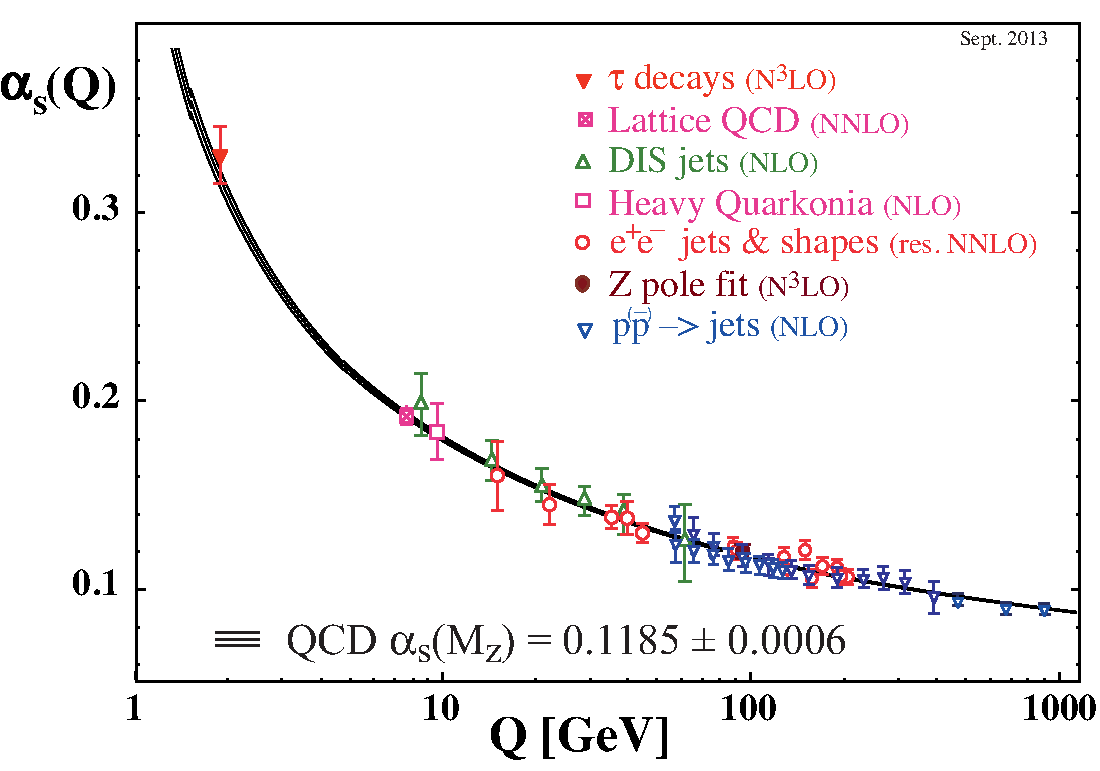
\includegraphics[width=0.8\textwidth]{figures/standardmodel/asq-2013}
  \caption{Latest summary of measurements of $\alpha_S$ as a function of the energy scale $Q$.
The respective degree of QCD perturbation theory used in the extraction of $\alpha_S$ is
indicated in parentheses. Figure and caption taken from Ref.~\cite{Agashe:2014kda}.
  \label{fig:running_coupling}}
\end{figure}

At very low energy scales, the running of the strong coupling constant results in a very large
value for $\alpha_S$. This explains the observation that no one has ever found a single free quark. 
They are always `confined' in colourless (white) hadrons, \ie bound states of quarks and/or
antiquarks.  A quark and antiquark of opposite colour (\eg $r$ and $\overline{r}$) can form a
\textit{meson} and 3 quarks of different colour ($r$, $g$ and $b$) can form a \textit{baryon}. 
Mesons and baryons are collectively referred to as \textit{hadrons}.
When one tries to separate two quarks, for example in a high energy collision, they behave like a
string, and energy is built up between them. At some point it becomes energetically more favourable
to use this energy to create extra quarks from the vacuum. 
This process is called hadronization and is responsible for the creation of \textsl{jets}, the
sprays of hadrons that are found at collider experiments. More information on hadronization is
presented in Section~\ref{sec:event_hadronization}.


\section{Brout-Englert-Higgs mechanism \label{sec:SM_HiggsMechanism}}

Introducing masses into a chiral theory is not a trivial issue, but is required to come to a viable
description of the elementary particles. 
The Brout-Englert-Higgs mechanism~\cite{Englert:1964et,Higgs:1964pj} accomplishes this by
introducing one or more scalar fields, the
Higgs fields, into the theory. These fields acquire a vacuum expectation value that spontaneously
breaks a symmetry in the Lagrangian. 
According to the Goldstone theorem, every spontaneously broken continuous symmetry
results in a massless scalar particle, the Goldstone boson. 
Hence, the number of Goldstone bosons in a theory is equal to the number of broken generators of
the symmetry group. 
However, in the case of a gauge theory, like the Standard Model, this is not the full story. 
We shall see that the massless gauge bosons of the theory acquire a mass by absorbing the Goldstone
bosons. 
The number of massive gauge bosons in a spontaneously broken gauge theory will thus be equal to the
number of broken generators. 


Before electroweak symmetry breaking, all four electroweak gauge bosons, $\W^1$, $\W^2$, $\W^3$,
and $B^0$, are massless. What we observe in experiment is one massless gauge boson, the photon
$\gamma$, and three massive gauge bosons ($\W^+, \W^-, \cPZ$). We also know that the electric charge
is conserved. The spontaneous symmetry breaking should thus be of the form
\begin{equation*}
  SU(2)_L \times U(1)_Y \rightarrow U(1)_{\text{EM}} \textrm{ .}
\end{equation*}

For three gauge bosons to acquire mass, three Goldstone bosons will have to be absorbed. As a
consequence, the scalar fields need to contain at least three degrees of freedom for the mechanism
to work. The simplest way to do this is by introducing a complex, scalar $SU(2)$ doublet $\Phi$ with
positive hypercharge ($Y = \frac{1}{2}$),
\begin{equation}
  \Phi = \begin{pmatrix} \phi^+ \\ \phi^0 \end{pmatrix} \textrm{ .} 
\end{equation}
The Standard Model Lagrangian without the strong part, \ie only the electroweak gauge bosons and
leptons, is given by
\begin{equation}
  \mathcal{L}_{SM} = - \frac{1}{4}W_{\mu\nu}^aW_a^{\mu\nu} - \frac{1}{4}B_{\mu\nu}B^{\mu\nu} +
\overline{L}_i (iD_\mu\gamma^\mu) L_i + \overline{e}_{R,i} (iD_\mu\gamma^\mu) e_{R,i} \textrm{ , } 
\end{equation}
where $i$ runs over the three generations, $\mu,\nu$ are Lorentz indices and $a$ runs over the
number of generators in the gauge group.
The field strengths are given by,
\begin{align*}
  W_{\mu\nu}^a &= \partial_\mu W_\nu^a - \partial_\nu W_\mu^a + g_2 \epsilon^{abc} W_\mu^b W_\nu^c
\textrm{ ,} \\
  B_{\mu\nu} &= \partial_\mu B_\nu - \partial_\nu B_\mu \textrm{ ,}
\end{align*}
and the covariant derivative for left- and right-handed leptons by,
\begin{align*}
  D_\mu L_L &= \left(\partial_\mu - i g_2 T_a W_\mu^a - i g_1 Y B_\mu \right) L_L \textrm{ ,}\\
  D_\mu e_R &= \left(\partial_\mu - i g_1 Y B_\mu \right) e_R \textrm{ ,}
\end{align*}
where $T_a$ are the generators of the $SU(2)_L$ gauge group and $g_1$, $g_2$ are the coupling
constants for the electroweak interaction.

Having introduced the scalar doublet $\Phi$, we need to add the corresponding scalar part to the
Lagrangian,
\begin{equation}
  \mathcal{L}_{S} = (D^\mu \Phi)^\dagger(D_\mu \Phi) - V(\Phi), \quad \textrm{with } V(\Phi) = \mu^2
\Phi^\dagger \Phi + \lambda (\Phi^\dagger \Phi)^2 \textrm{ . } 
  \label{eq:scalarlagr}
\end{equation}
The first term is the kinetic term and the second term is the scalar potential, which is often
called the ``Mexican Hat'' potential. The form of the Higgs potential is an assumption in the
Standard Model. It is not known from first principles, but is rather chosen for its nice
properties. It is the simplest potential that can achieve the necessary spontaneous symmetry
breaking, while being renormalizable.  
In order for the vacuum to be stable, the parameter $\lambda$ has to be positive. Depending on the
sign of $\mu^2$ one can distinguish two cases, which are illustrated in
Fig.~\ref{fig:Higgs_potential}. 
In the case $\mu^2 > 0$, the potential $V(\Phi) = \mu^2 \Phi^\dagger \Phi + \lambda (\Phi^\dagger
\Phi)^2$ is always positive with a the minimum  at 
\begin{equation}
\braket{0|\Phi|0} \equiv \Phi_0 = \begin{pmatrix}0\\0\end{pmatrix}. 
\end{equation}
Since the minimum is at the origin, no spontaneous symmetry breaking takes place. 
In case $\mu^2 < 0$, the minimum of the potential is no longer located at the origin. Therefore, the
neutral component of the scalar field can acquire a vacuum expectation value (vev) $v$, thereby
breaking the electroweak symmetry.
\begin{equation}
  \braket{0|\Phi|0} \equiv \Phi_0 = \begin{pmatrix} 0 \\ \frac{v}{\sqrt{2}} \end{pmatrix} \textrm{ ,
} \quad v = \sqrt{- \frac{\mu^2}{\lambda}} \textrm{ .}
\end{equation}
By only giving a vev to the neutral component, electromagnetism is conserved, as we set out
to achieve. 

\begin{figure}[htb]
  \centering
  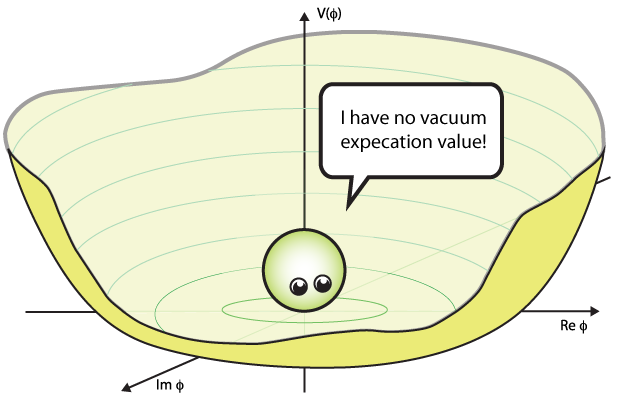
\includegraphics[width=0.48\textwidth]{figures/standardmodel/BoringPotential}
  
  \vspace{2eM}
  
  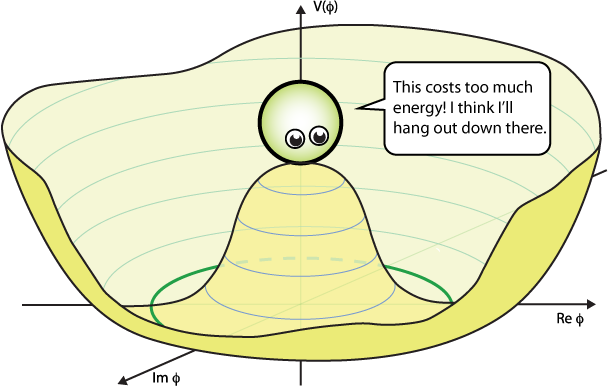
\includegraphics[width=0.48\textwidth]{figures/standardmodel/Higgs-Potential-lookdown}
  ~
  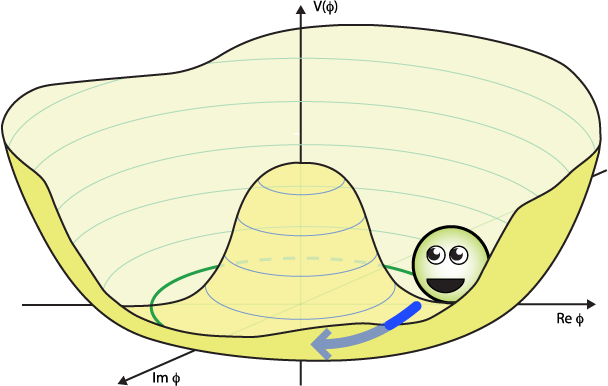
\includegraphics[width=0.48\textwidth]{figures/standardmodel/Higgs-Potential-Goldstone}
  \caption{ [top] The scalar potential with $\mu^2 > 0$ is always positive, with minimum in the
origin. The scalar field will obtain a vacuum expectation value of zero. 
  [bottom] The scalar potential with $\mu^2 < 0$ has a ``Mexican hat'' shape, with the minimum in a
rim around the origin. The scalar field will thus move from the origin down to the actual minimum
and acquire a non-zero vev in the process. The green line indicates a flat direction in the
potential,
corresponding to a massless Goldstone mode.
  Figures taken from Ref.~\cite{Higgs_potential}.
  \label{fig:Higgs_potential}}
\end{figure}

We proceed by expanding $\Phi$ around its minimum $\Phi_0$
\begin{equation}
  \Phi(x) = \frac{1}{\sqrt{2}} \binom{0}{ v + H(x) } \textrm{ ,}
  \label{eq:higgsexpansion}
\end{equation}
where we have introduced a new scalar field $H(x)$.
After inserting this in the kinetic part of the scalar Lagrangian (Eq.~\ref{eq:scalarlagr}), and
redefining the gauge fields as
\begin{align}
  W^\pm_\mu &= \frac{1}{\sqrt{2}} (W_\mu^1 \mp i W_\mu^2), \\
  Z_\mu &= \frac{1}{\sqrt{g_1^2 + g_2^2}} (g_2W_\mu^3 - g_1 B_\mu),\\
  A_\mu &= \frac{1}{\sqrt{g_1^2 + g_2^2}} (g_2W_\mu^3 + g_1 B_\mu) ,
\end{align}
we find for the kinetic part of the scalar Lagrangian,
\begin{equation}
  |D_\mu \Phi|^2 = \frac{1}{2} (\partial_\mu H)^2 + \frac{1}{2}g_2^2(v+H)^2 W^+_\mu W^{\mu -} +
\frac{1}{8}(v+H)^2 (g_1^2 + g_2^2) Z_\mu Z^\mu \textrm{ .}
\end{equation}
We see that the photon $A_\mu$ remains massless, as required for an unbroken symmetry. Mass terms
for the $W$ and $Z$ bosons have the general form $M_W^2 W_\mu W^\mu$ and $ \frac{1}{2} M_Z^2 Z_\mu
Z^\mu$. We thus find for the gauge boson masses,
\begin{align}
  M_W &= \frac{1}{2} v g_2 ,\\
  M_Z &= \frac{1}{2} v \sqrt{g_1^2 + g_2^2}, \\
  M_A &= 0 \textrm{ .}
\end{align}
After spontaneous symmetry breaking, three gauge bosons have thus absorbed a degree of freedom from
the scalars (corresponding to the would-be Goldstone bosons), becoming massive in the process. One
massless gauge boson and one scalar remain.
The remaining scalar degree of freedom $H$ corresponds to the so-called Higgs boson. 

The mixing resulting in orthogonal combinations for the photon and $\cPZ$ bosons is often described
in terms of the Weinberg or weak mixing angle, $\theta_W$,
\begin{align}
  A_\mu &=  \cos \theta_W B_\mu + \sin \theta_W W_\mu^3,\\
  Z_\mu &=  - \sin \theta_W B_\mu + \cos \theta_W W_\mu^3, 
\end{align}
with the Weinberg angle itself defined as
\begin{equation}
  \sin \theta_W = \frac{g_1}{\sqrt{g_1^2 + g_2^2}} .
\end{equation}
At tree level, we also find a relation between the masses of the $\W$ and $\cPZ$ bosons: 
\begin{equation}
  \frac{M_\W}{M_\cPZ} = \frac{g_2}{\sqrt{g_1^2 + g_2^2}} = \cos \theta_W . 
\end{equation}
The precise measurement of the $\W$ and $\cPZ$ boson masses can thus be used to measure the Weinberg
angle.
Working through the interaction terms between the photon and the fermions, one can show that the
weak mixing angle relates the coupling strength of the weak interaction to that of the
electromagnetic interaction, 
\begin{equation}
  e = g_2 \sin \theta_W .
\end{equation}

The mass and
couplings of the Higgs boson $H$ can be determined from the scalar Lagrangian,
Eq.~\ref{eq:scalarlagr}, upon substituting Eq.~\ref{eq:higgsexpansion}. 
Using $v^2 = -\frac{\mu^2}{\lambda}$ and extracting the parts containing only $H$, we find for the
Lagrangian of the Higgs boson:
\begin{equation}
  \mathcal{L}_H = \frac{1}{2} (\partial_\mu H)(\partial^\mu H) - \lambda v^2 H^2 - \lambda v H^3 -
\frac{\lambda}{4} H^4 \textrm{ .}
\end{equation}
Scalar masses have the general form $\frac{1}{2} m \phi^2$; the Higgs boson mass is thus
\begin{equation}
m_H =  2 \lambda v^2 = - 2 \mu^2,
\end{equation}
and needs to be determined experimentally since there is no other way to access the parameter
$\lambda$. 

Now that we have generated masses for the gauge bosons, all we still need to do, is
generate masses for the fermions as well. This can be done by introducing Yukawa coupling terms
between the fermions and the Higgs fields. 
The Yukawa Lagrangian for the first generation is given by
\begin{equation}
  \mathcal{L}_F = - \lambda_e \overline{L} \Phi e_R - \lambda_d \overline{Q} \Phi d_R - \lambda_u
\overline{Q} \widetilde{\Phi} u_R + h.c. \textrm{ ,}
  \label{eq:Lag_Yuk}
\end{equation}
where we introduced the conjugate of $\Phi$, $\widetilde{\Phi} = i \tau_2 \Phi^*$ which has negative
hypercharge. 
This is needed in order to enable the coupling of the Higgs field to the up-type quarks.
It is also possible to
introduce a completely new Higgs doublet with negative hypercharge. This kind of model is called a
two-Higgs doublet model (2HDM) and is needed to introduce supersymmetry (see
Chapter~\ref{chap:supersymmetry}). 

Substituting (\ref{eq:higgsexpansion}) in (\ref{eq:Lag_Yuk}), we find 
\begin{align}
  \mathcal{L}_F &= - \frac{1}{\sqrt{2}} \lambda_e (\overline{\nu}_e, \overline{e}_L) 
		  \begin{pmatrix}0 \\ v+H \end{pmatrix} e_R + ... \\
                &= - \frac{1}{\sqrt{2}} \lambda_e (v+H) \overline{e}_L e_R + ... \textrm{ ,}
  \label{eq:yukawa}
\end{align}
where we highlighted the electron part. 
Fermion mass terms have the general form $m_f \overline{f}_L f_R + h.c.$. We find
\begin{equation}
m_e = \frac{\lambda_e v}{\sqrt{2}}, \qquad m_u = \frac{\lambda_u v}{\sqrt{2}}, \qquad m_d =
\frac{\lambda_d v}{\sqrt{2}}. \label{eq:fermion_masses}
\end{equation}
The neutrinos are seen to remain massless as a result of the lack of a right-handed neutrino in the
Standard Model. 

Using the same doublet of scalar fields we have thus successfully given mass to the gauge bosons and
fermions in our theory. The Brout-Englert-Higgs mechanism also predicts the existence of a massive
scalar particle, the Higgs boson. 
When in 2012 a particle with all the characteristics of this Higgs boson was found at the LHC, this
meant the verification that the process of electroweak symmetry breaking is indeed realized in
nature. 


\section{A success story \label{sec:SM_success}}

Since its conception decades ago, the Standard Model has performed beyond anyone's expectation. 
It has provided an accurate description of results from many accelerator and non-accelerator based
experiments. In this section I will highlight the latest achievement, the discovery of the Higgs
boson, and a global test of the validity of the Standard Model via electroweak precision fits. 

\subsection{Higgs boson discovery}

The existence of the Higgs boson was first proposed in 1964 by Robert Brout and Fran\c{c}ois
Englert~\cite{Englert:1964et}, and independently also by Peter Higgs~\cite{Higgs:1964pj}, and
Gerald Guralnik, Richard Hagen and Tom Kibble~\cite{Guralnik:1964eu}. 
Nearly half a century later, on the fourth of July, 2012, its discovery was finally announced by the
CMS and ATLAS Collaborations at the LHC.

The allowed mass range for the Higgs boson had already been narrowed down by the experiments at LEP
and the Tevatron, and by the dataset delivered by the LHC in 2011 at a centre-of-mass energy of
7\TeV. 
In that latter dataset, some evidence for a particle with a mass around 125\GeV was already
observed~\cite{Chatrchyan:2012tx}, although not strong enough to claim a discovery. 
The energy increase to 8\TeV in 2012 provided just the boost needed to claim
discovery with $5\sigma$ significance~\cite{Chatrchyan:2012ufa}. The evidence was strongest in the
decay channels $H\rightarrow\gamma\gamma$ and $H\rightarrow\cPZ\cPZ^*\rightarrow 4\ell$.
Figure~\ref{fig:higgs_discovery} shows the invariant mass distributions of the diphoton and
four-lepton systems obtained by the CMS experiment. There is an excess visible around 125\GeV. 
The final Higgs boson mass measurement for Run 1 at CMS, combining all decay channels, and combining
the 7\TeV and 8\TeV datasets, which correspond to an integrated luminosity of 5.1\fbinv and
19.7\fbinv, respectively, 
found the following value for the Higgs boson mass,
\begin{equation}
  m_H = 125.02 {\,}^{+0.26}_{-0.27} \, (\text{stat}) {\,}^{+0.14}_{-0.15} \, (\text{syst}) \GeV.
\end{equation}
The measured cross section $\sigma$ also agrees very well with the expectation from the Standard
Model. The signal strength at the measured mass was measured from the combination of all decay
channels, and found to be
\begin{equation}
 \frac{\sigma}{\sigma_{\text{SM}}} = 1.00 \pm 0.09 \, (\text{stat})
{\,}^{+0.08}_{-0.07} \, (\text{theory}) \pm 0.07 \, (\text{syst}) .
\end{equation}
Many more tests of the properties of the observed particle have been
made~\cite{Khachatryan:2014jba}. Examples are the spin and parity of the particle, the ratios of
production rates for different production modes, the ratios of couplings to fermions and vector
bosons, and the possible branching fraction to non-SM particles, $\text{BR}_{\text{BSM}}$. 
A subset of these measurements is shown in Fig.~\ref{fig:higgs_sm_test}. The $\kappa$ variables
are the (effective) coupling strength modifiers \wrt the SM Higgs boson couplings. The couplings to
massive vector bosons, fermions, gluons and photons are denoted by $\kappa_{\text{V}}$,
$\kappa_{\text{f}}$, $\kappa_{\text{g}}$ and $\kappa_\gamma$, respectively.
The ratios of separate coupling strength modifiers are denoted by $\lambda_{\text{XY}} =
\kappa_{\text{X}}/\kappa_{\text{Y}}$. Figure~\ref{fig:higgs_sm_test} includes the ratio of
couplings to $\W$ and $\cPZ$ bosons, $\lambda_{\text{WZ}}$, the ratio between down- and up-type
quarks, $\lambda_{\text{du}}$, and the ratio of couplings between leptons and quarks,
$\lambda_{\text{lq}}$. 
Excellent agreement with the Standard Model expectation is found.

\begin{figure}[p]
  \centering
  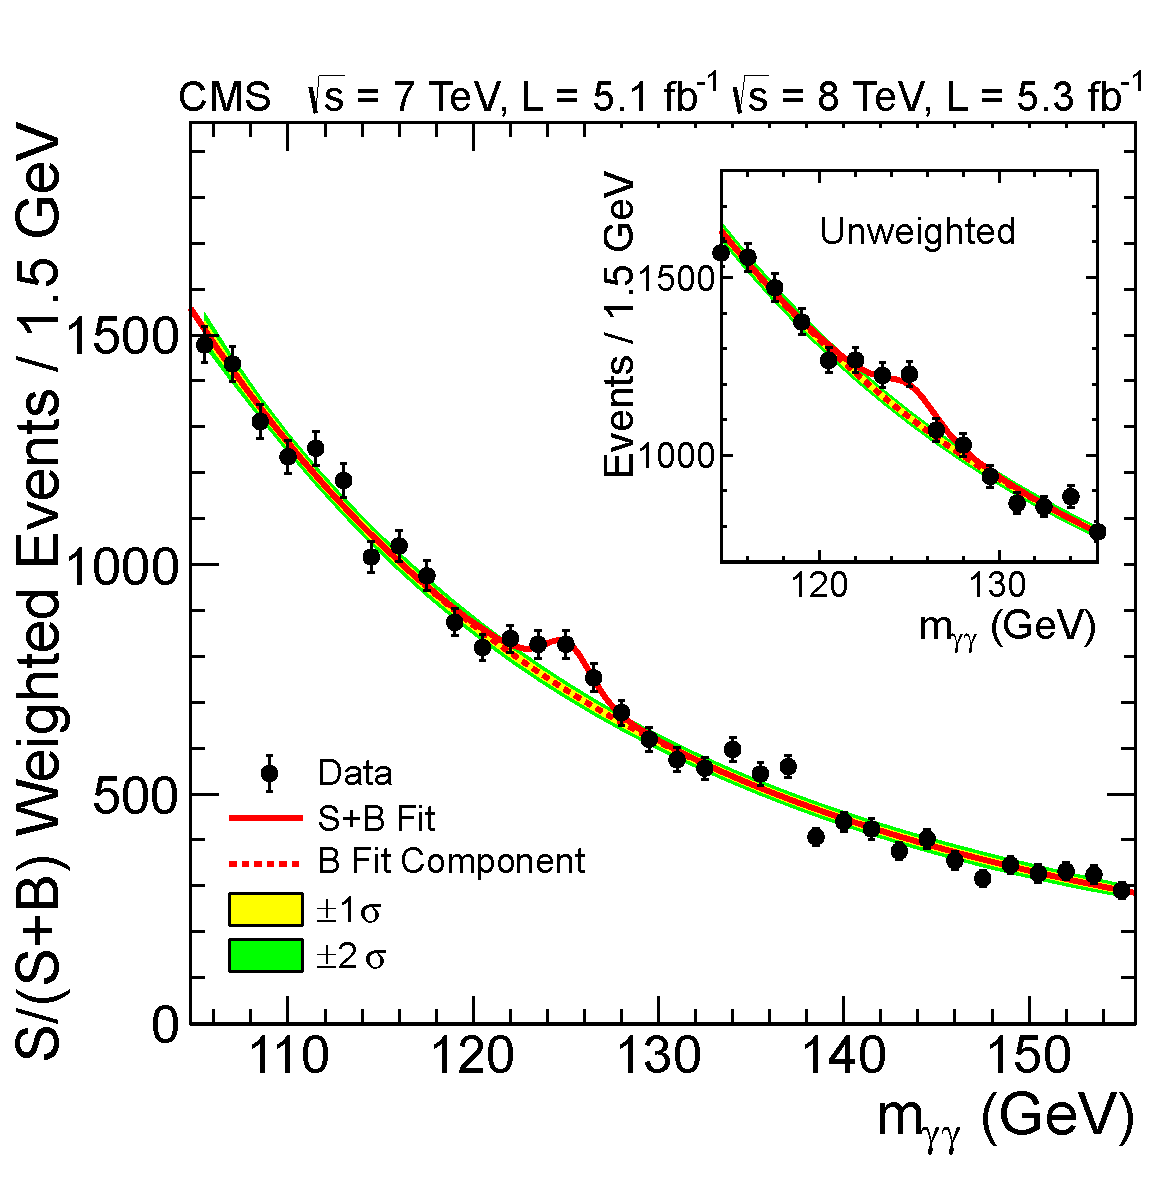
\includegraphics[height=0.29\textheight]{figures/standardmodel/higgs_diphoton}
  ~
  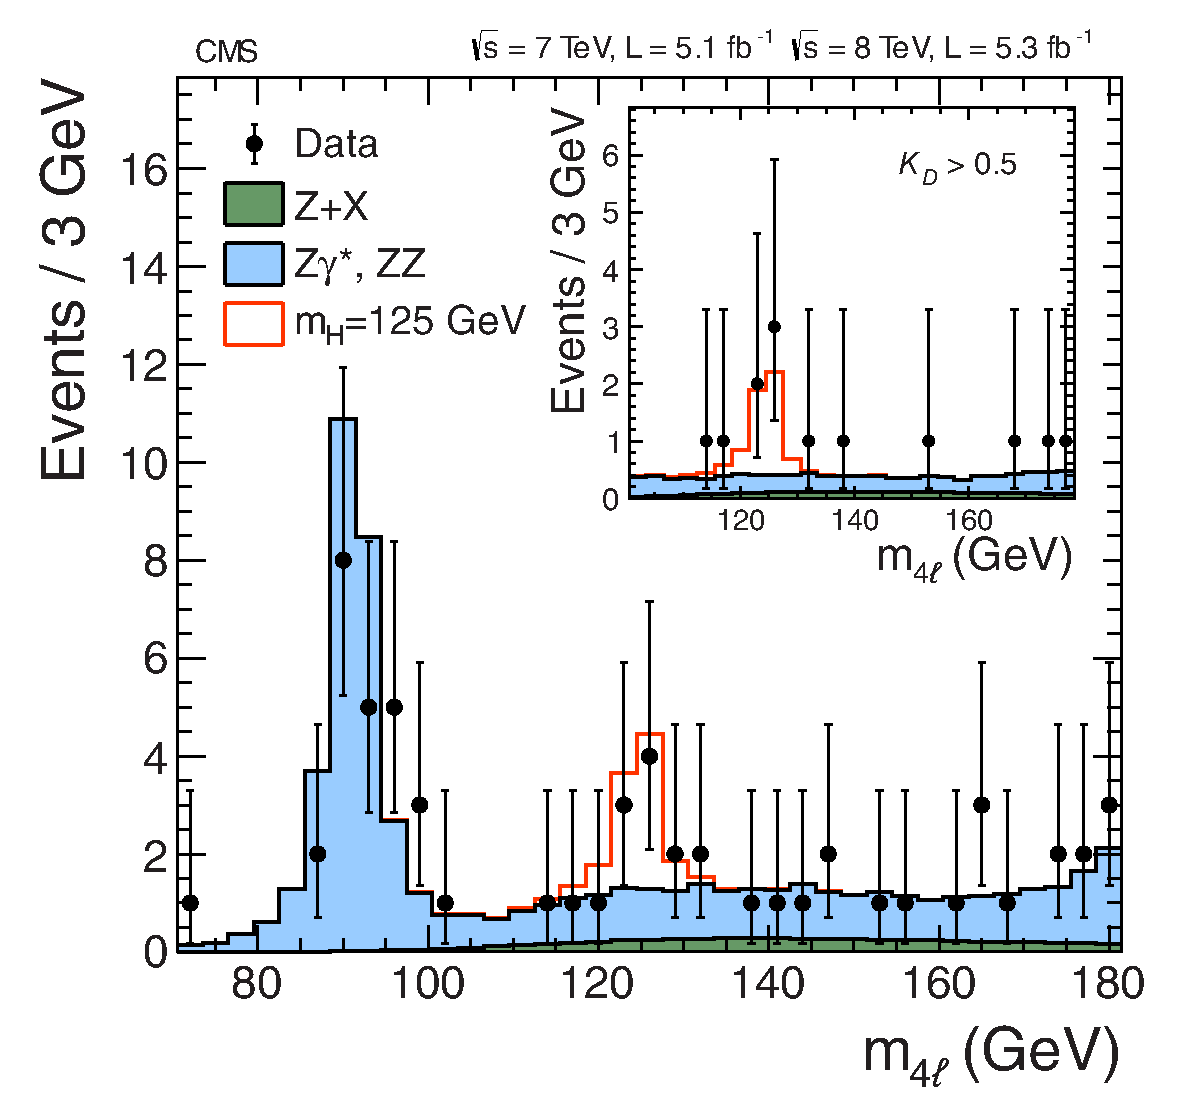
\includegraphics[height=0.28\textheight]{figures/standardmodel/higgs_fourlepton}
  \caption{The Higgs discovery in the two high-resolution channels. Figures taken from
Ref.~\cite{Chatrchyan:2012ufa}.
  [left] The diphoton invariant mass distribution with each event weighted by the
$\frac{S}{S+B}$ value of its selection category. The lines represent the fitted background and
signal, and the coloured bands represent the $\pm$1 and $\pm$2 standard deviation uncertainties in
the background estimate. 
  [right] Distribution of the four-lepton invariant mass for the $\cPZ\cPZ^* \rightarrow 4\ell$
analysis. The points represent the data, the filled histograms represent the background, and the
open histogram shows the signal expectation for a Higgs boson of mass $m_H = 125\GeV$, added to the
background expectation.
  \label{fig:higgs_discovery}}
\end{figure}

\begin{figure}[p]
  \centering
  \vspace{1ex}
  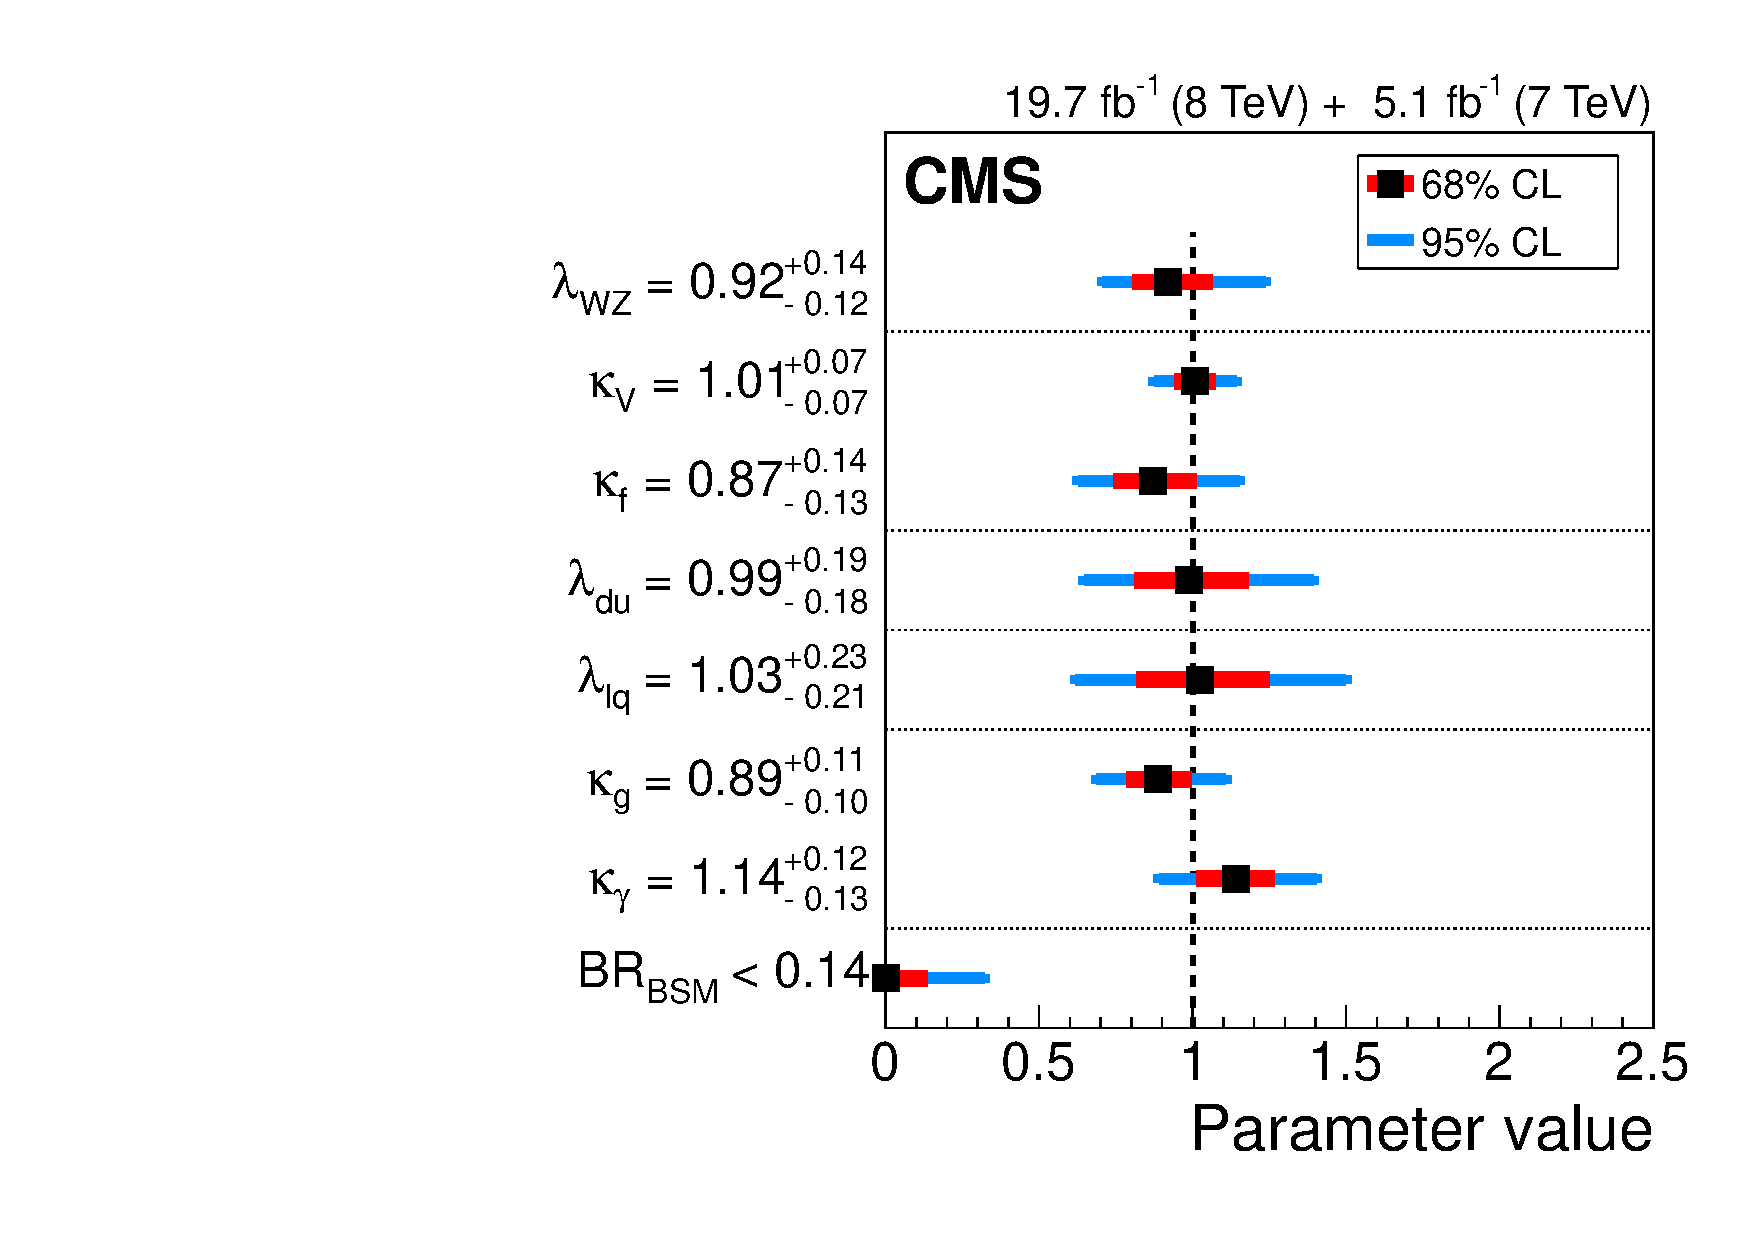
\includegraphics[width=0.65\textwidth]{figures/standardmodel/sqr_summary_lhcxswg}
  \caption{ Summary of tests of the compatibility of the CMS data with the SM Higgs boson
couplings as discussed in the text.
The observed boson is fully compatible with the Standard Model expectation. Figure taken
from Ref.~\cite{Khachatryan:2014jba}.
  \label{fig:higgs_sm_test}}
\end{figure}


\subsection{Precision electroweak fits}

Electroweak precision observables can probe energy scales much larger than what is possible in
direct measurements, through the effects of higher-order corrections. 
Therefore, measurements of these observables at lepton colliders such as LEP and SLC, along with
measurements at hadron colliders, such as the Tevatron and LHC, need to be paired with
very accurate theoretical predictions.
Up until the Higgs boson discovery, this experimental and theoretical input was used in global fits
of the electroweak sector in order to constrain the free parameters of the Standard Model.
Now, on the other hand, assuming that the newly discovered Higgs boson is indeed the SM Higgs boson,
all fundamental parameters that are used in the fit are known, and the fit is overconstrained. This
means that we can now fully test the consistency of the Standard Model, as well as predict some of
the observables with higher precision than the direct measurements. 
There are several groups performing these global
fits~\cite{CKMFitter,GFitter,ZFitter,LEPEWWG}. I will take the latest results from the GFitter
group~\cite{Baak:2014ora,Flacher:2008zq} as illustration here.

% \begin{wrapfigure}{r}{0.5\textwidth}
% \includegraphics[width=0.5\textwidth]
% {figures/standardmodel/2014_07_16_PullPlotTwoBarsTwoTheos_logo}
% \caption{ Comparison of the GFitter fit results with the direct measurements in units of the
% experimental uncertainty. 
% Figure from Ref.~\cite{Baak:2014ora}.
% \label{fig:global_fit1}}
% \end{wrapfigure}
The measurements that are used in the fit include, among others, the mass of the Higgs boson, the
mass and width of the $\W$ and $\cPZ$ bosons, the mass of the top, bottom and charm quarks, the
strong coupling constant, the forward-backward asymmetry and asymmetry parameters for leptons,
$\cPqc$ and $\cPqb$ quarks, and the weak mixing angle. 
Several of the theoretical predictions that are used in the fit procedure are now known up to two
or more loop orders. Examples are the effective weak mixing angle, the mass of the $\W$ boson, and
the partial widths and branching ratios of the $\cPZ$ boson. 

\begin{figure}[p]
\centering
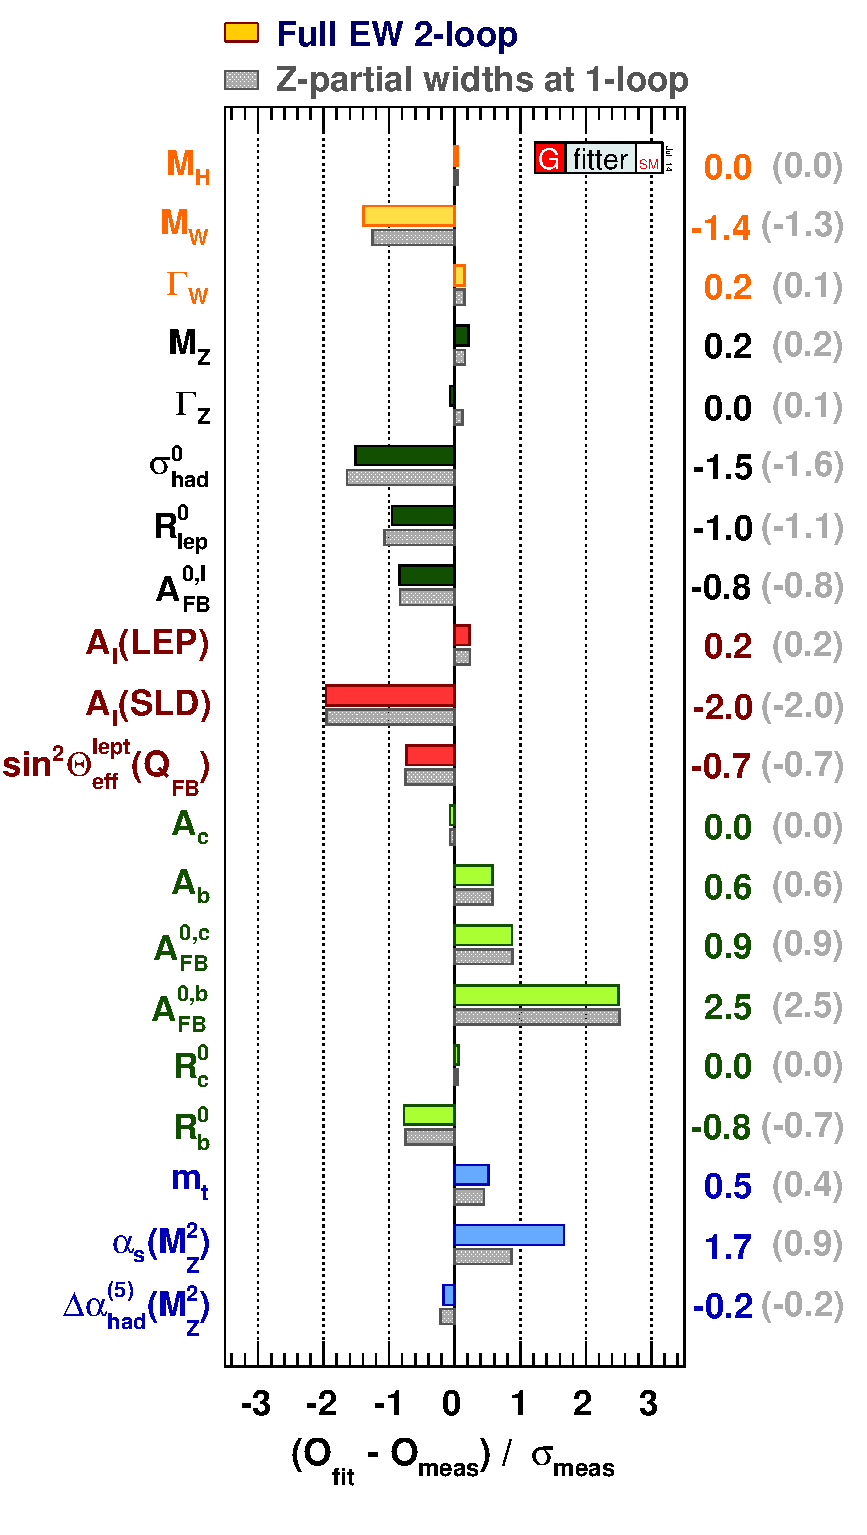
\includegraphics[height=0.8\textheight]
{figures/standardmodel/2014_07_16_PullPlotTwoBarsTwoTheos_logo}
\caption{ Comparison of the GFitter fit results with the direct measurements in units of the
experimental uncertainty. 
Figure from Ref.~\cite{Baak:2014ora}.
\label{fig:global_fit1}}
\end{figure}

Figure~\ref{fig:global_fit1} shows the comparison of the fit results with the direct measurements.
The agreement is within three standard deviations for all observables. 
An important consistency test of the SM is the simultaneous indirect determination of
the top and $\W$ boson mass. The top plot in Fig.~\ref{fig:global_fit} shows a scan of the
confidence level profile of $m_\W$ versus $m_\cPqt$ for the scenarios where the direct Higgs mass
measurement is included in the fit (blue) or not (grey). Both contours agree with the direct
measurements shown in the green bands and ellipses. The corresponding plot for the effective weak
mixing angle and the $\W$ boson mass is shown on the bottom of Fig.~\ref{fig:global_fit}. 
The agreement between the indirect determination via the fit procedure and the direct measurement,
is very good, showing the consistency of the Standard Model with experiment. 


\begin{figure}[p]
  \centering
  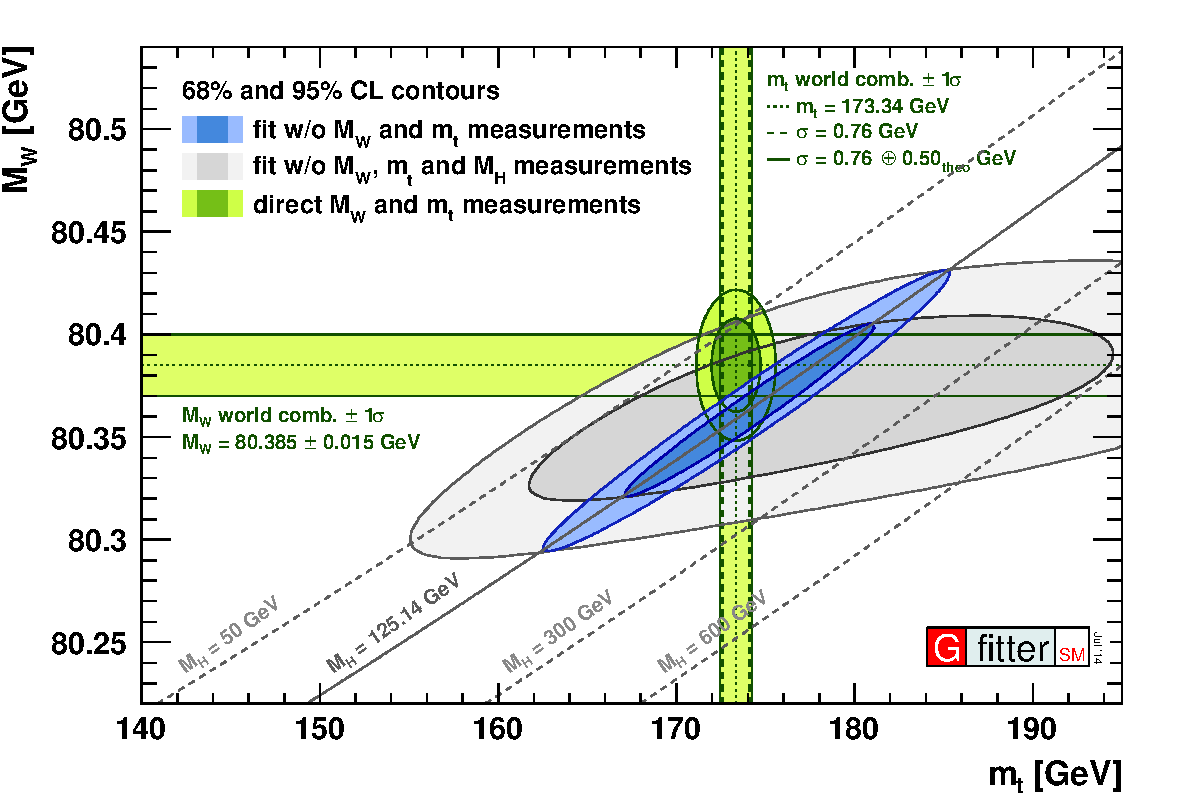
\includegraphics[width=0.8\textwidth]{figures/standardmodel/2014_07_16_Scan2D_MWvsmt_logo}
  
  \vspace{1eM}
  
  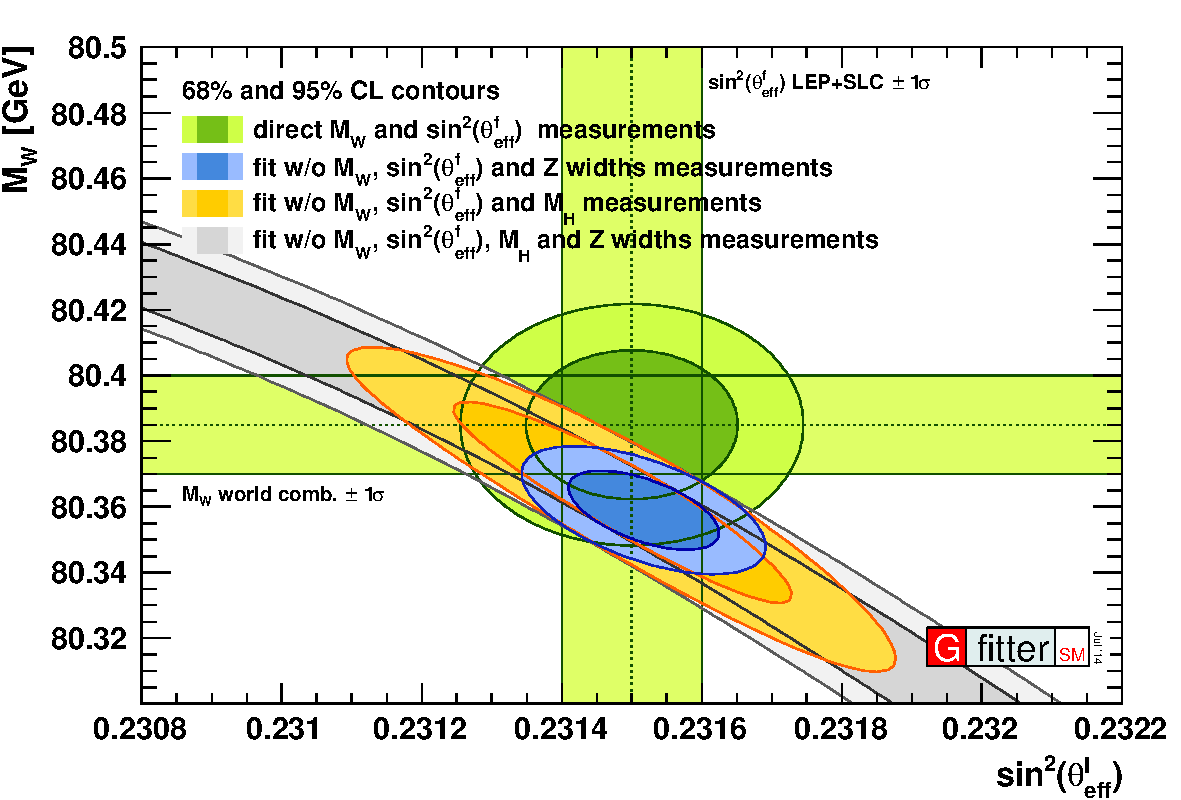
\includegraphics[width=0.8\textwidth]{figures/standardmodel/2014_07_16_Scan2D_MWvsSinEffLep_logo}
\caption{Contours at 68\% and 95\% confidence level obtained from scans of $m_\W$ versus $m_\cPqt$
(top) and $m_W$ versus $\sin^2 (\theta^l_{\text{eff}})$ (bottom), for a fit including $m_H$ (blue)
and excluding $m_H$ (grey), as compared to the direct measurements (vertical and horizontal green
bands and ellipses). In both figures, the corresponding direct measurements are excluded
from the fit. Figures and caption from Ref.~\cite{Baak:2014ora}.
\label{fig:global_fit}}
\end{figure}




\chapter{The need for physics beyond the Standard Model \label{chap:beyond_standard_model}}

Although the Standard Model has succeeded in predicting and explaining a plethora of physics
processes, it cannot be the ultimate theory describing Nature. In
Section~\ref{sec:missing_elements}, I will list some open questions for which the Standard Model
does not provide an answer. A very pertinent question regarding the Higgs boson mass is discussed
in Section~\ref{sec:hierarchy_problem}.
Any new theory that attempts to solve these issues should reproduce
the Standard Model for the energy domains that have been so thoroughly tested over the past
decades. In this respect we can view the Standard Model as an effective low-energy theory, just
like Newton's laws of motion follow from a low-energy approximation of special relativity. 
Most of the proposed new physics theories are, therefore, extensions of the Standard Model. 
A number of possibilities are introduced in Section~\ref{sec:extensions_standard_model}.

\section{Open questions \label{sec:missing_elements}}

The open questions can roughly be divided in two categories. The first category comprises the
experimental observations that are not covered at all by the SM, while the second category concerns
characteristics of the SM for which we have no fundamental explanation. 
I provide a non-exhaustive list below.

\paragraph{Category 1}
\begin{itemize}
  \item \textbf{Gravity} is not included in the Standard Model. The main reason for this is that
a satisfactory microscopic theory of gravity has not been formulated yet. Some advances have been
made, \eg supergravity
theories~\cite{VanNieuwenhuizen:1981ae,freedman2012supergravity,Nastase:2011aa}, but it is not yet
at the point where it can be unified with the rest of the Standard Model. 

  \item The latest Planck results~\cite{Planck:2015xua} state that about 26\% of the energy budget
of the universe is covered by \textbf{dark matter}, compared to less than about 5\% for the ordinary
matter that is described by the Standard Model. Currently, the Standard Model does not contain any
particle that could be a dark matter candidate. Such a particle should be stable, neutral, weakly
interacting and have a reasonably large mass. 

  \item In addition to the presence of dark matter, we have very strong indications that
the remaining 69\% of the universe is \textbf{dark energy}, and drives the expansion of the
universe. The Planck results also indicate that this dark energy is consistent with the assumption
of a cosmological constant. The SM again does not provide an explanation for this, in fact, any
attempt to compute this cosmological constant in terms of vacuum energy leads to a mismatch of
around 100 orders of magnitude. 

  \item The universe is almost entirely made up of matter, rather than antimatter. Assuming that
equal amounts were created in the Big Bang, the SM cannot explain this \textbf{matter-antimatter
asymmetry}. As postulated by Sakharov~\cite{Sakharov}, there are three necessary conditions for a
baryon asymmetry to exist: charge (C) and charge-parity (CP) violation; the absence of thermal
equilibrium; and at least one baryon number violating process. Within the SM there is a small amount
of CP violation, \eg in the decay of the $K^0$ meson. However, even if the other two conditions were
satisfied, there would not be enough CP violation to explain the observed matter-antimatter
discrepancy. 
  
  \item Neutrinos of different flavour have been observed to
oscillate~\cite{Abe:2008aa,Abe:2014ugx,Agafonova:2014ptn}. These \textbf{neutrino oscillations} can
only occur if at least two of the three neutrino types have mass. The neutrino mass eigenstates
($\nu_1, \nu_2, \nu_3$) are then superpositions of the flavour eigenstates ($\nu_e, \nu_\mu,
\nu_\tau$).
No measurements of the absolute masses have been made so far, but the squared mass differences are
known. 
In the Standard Model the neutrinos are massless. Adding a mass to the neutrinos can be
done~\cite{Klinkhamer:2011aa}, but the question remains whether they are normal Dirac fermions, or
Majorana fermions (\ie their own antiparticle). 
\end{itemize}

\paragraph{Category 2}

\begin{itemize}
  \item Why is the Higgs boson mass only 125\GeV? Radiative corrections would automatically drive
this mass up to very large scales. This is often referred to as the hierarchy problem.
As we will see later, this issue forms part of the motivation for the search presented in this
thesis, and will thus be covered in some more detail in Section~\ref{sec:hierarchy_problem}. 

  \item Why are there three families of fermions? Careful study of the lineshape of the $\cPZ$
boson has shown that there is no fourth family with light neutrinos~\cite{Decamp:1989fr}. Could
there be an extra family with heavier neutrinos?

  \item Why do the fermions have the masses, \ie couplings to the Higgs boson, they have? And why
is there such a wide range of masses, \ie from $0.511\MeV$ for the electron up to 173\GeV for the
top quark, a difference of 5 orders of magnitude. This is sometimes referred to as the fermion mass
hierarchy problem. 

  \item Are baryon and lepton numbers conserved? In the Standard Model these are accidental
symmetries, without an underlying reason such as a local gauge symmetry. There is thus no
compelling reason to assume that baryon and lepton number are conserved quantities. 
  
  \item Why is the $\mu^2$ parameter in the Higgs potential ($\mu^2 \Phi^\dagger \Phi + \lambda
(\Phi^\dagger \Phi)^2$) negative? Within the SM this is an assumption that is made, without
underlying motivation other than that it is needed to trigger electroweak symmetry breaking.
\end{itemize}


\section{The hierarchy problem \label{sec:hierarchy_problem}}

At the core of the hierarchy problem are the different mass scales that are present in the
universe. The Standard Model does a very good job explaining phenomena at the electroweak scale of
$\mathcal{O}(100\GeV)$. We know that when we reach the Planck scale,
$\mathcal{O}(\text{10}^{\text{19}}\GeV)$, the SM can no longer be the complete theory, as 
quantum gravity effects will then need to be included. 

Observed particle masses are a combination of the bare, tree-level mass, and all radiative
corrections from additional loop diagrams. The loop momenta are cut off at the scale where we
believe the theory to be no longer valid, in this case the Planck scale. 
For fermion masses these corrections are only logarithmically dependent on the high cutoff scale,
as they are protected by chiral symmetry. Gauge bosons are similarly protected by the local gauge 
symmetry. The Higgs boson, being a scalar, does not have any protection, and therefore the
radiative corrections introduce a quadratic dependence on the cutoff scale. 

The one-loop corrections to the Higgs boson mass arise from the diagrams shown in
Fig.~\ref{fig:oneloopdiagrams}. The fermionic loop correction arises from the Yukawa interaction
between the Higgs boson and the fermions. The relevant part of the Lagrangian (Eq.~\ref{eq:yukawa})
is given for a generic fermion as,
\begin{equation}
  \mathcal{L}_{f\bar{f}H} = - \frac{\lambda_f}{\sqrt{2}} H f \bar{f} .
\end{equation}
When one computes the fermionic one-loop diagram, we find for the correction to the Higgs boson
mass~\cite{Djouadi:2005gj}, 
\begin{equation}
  \Delta m_H^2 = N_f \frac{\lambda_f^2}{8\pi^2} \left[ - \Lambda^2 + 6 m_f^2 \log
\left(\frac{\Lambda}{m_f}\right) - 2 m_f^2 \right] + \mathcal{O}\left(\frac{1}{\Lambda^2}\right) ,
\end{equation}
where the quadratic dependence on the cutoff scale $\Lambda$ is explicitly visible. Taking this
cutoff to be the Planck scale results in a correction that is more than 30 orders of magnitude
larger than the Higgs boson mass squared itself. To still achieve an observable mass of 125\GeV, the
bare mass and the correction would thus have to cancel to an extremely high precision. The inclusion
of the vector boson and Higgs self-coupling loops do not change this overall behaviour. 
The requirement for this large amount of finetuning is viewed to be unnatural, and many models of
new physics will use the \textit{naturalness} argument in their favour. 

\begin{figure}[t]
\begin{tikzpicture}[scale=0.9]
  \node[void] (in) at (0,0)  {};
  \node[void] (v1) at (1,0) {};
  \node[void] (v2) at (2,0) {};
  \node[void] (out) at (3,0) {};
  \draw[spin0] (in) -- node [above]{$H$} (v1) ;
  \draw (1.5,0) circle (0.5);
  \node at (1.5,0.7) {$f$};
  \draw[spin0] (v2) -- node [above]{$H$} (out);
\end{tikzpicture}
\hfill
\begin{tikzpicture}[scale=0.9]
  \node[void] (in) at (0,0)  {};
  \node[void] (v1) at (1,0) {};
  \node[void] (v2) at (2,0) {};
  \node[void] (out) at (3,0) {};
  \draw[massvect] (v1) arc(180:0:0.5) ;
  \node at (1.5,0.8) {$W,Z$};
  \draw[spin0] (in) -- node [above]{$H$} (v1) -- (v2) -- node [above]{$H$} (out);
\end{tikzpicture}
\hfill
\begin{tikzpicture}[scale=0.9]
  \node[void] (in) at (0,0)  {};
  \node[void] (v1) at (1,0) {};
  \node[void] (v2) at (2,0) {};
  \node[void] (out) at (3,0) {};
  \draw[massvect] (1.5,0.45) circle (0.5);
  \node at (1.5,1.3) {$W,Z$};
  \draw[spin0] (in) -- node [above]{$H$} (v1) -- (v2) -- node [above]{$H$} (out);
\end{tikzpicture}
\hfill
\begin{tikzpicture}[scale=0.9]
  \node[void] (in) at (0,0)  {};
  \node[void] (v1) at (1,0) {};
  \node[void] (v2) at (2,0) {};
  \node[void] (out) at (3,0) {};
  \draw[spin0] (1.5,0.5) circle (0.5);
  \node at (1.5,1.3) {$H$};
  \draw[spin0] (in) -- node [above]{$H$} (v1) -- (v2) -- node [above]{$H$} (out);
\end{tikzpicture}
\caption{One-loop quantum corrections to the Higgs boson mass. From left to right: contribution
from the Yukawa interaction; two contributions from the gauge interaction; contribution from the
Higgs self-interaction.
\label{fig:oneloopdiagrams}}
\end{figure}

A way to remove this quadratic dependence on the cutoff scale is to introduce extra particles in
the theory, with properties such that the loop behaviour is opposite to the Standard Model
particles. It is straightforward to show that we can cancel the fermionic loops by introducing
extra scalar particles. 
Assuming that there are $N_S$ new scalar particles, with mass $m_S$, trilinear coupling $v\lambda_S$
and quadrilinear coupling $\lambda_S$, we find as additional contribution to the
one-loop correction to the Higgs mass:
\begin{multline}
  \Delta m_H^2 =  \frac{N_S\lambda_S}{16\pi^2} \left[ - \Lambda^2 + 2 m_S^2 \log
\left(\frac{\Lambda}{m_S}\right)\right] \\ - \frac{\lambda_S^2 N_S}{16 \pi^2} v^2 \left[ -1 + 2
\log\left(\frac{\Lambda}{m_S}\right) \right] + \mathcal{O}\left(\frac{1}{\Lambda^2}\right) .
\end{multline}
By assuming $\lambda_f^2 = - \lambda_S$ and $N_S = 2 N_f$, we find upon adding both
contributions, and using Eq.~\ref{eq:fermion_masses},
\begin{equation}
  \Delta m_H^2 = \frac{\lambda_f^2 N_f}{4\pi^2} \left[ \left(m_f^2-m_S^2\right)
\log\left(\frac{\Lambda}{m_S}\right) + 3 m_f^2 \log\left(\frac{m_S}{m_f}\right) \right] .
\end{equation}
All quadratically divergent terms have vanished. Introducing scalar particles with the
appropriate couplings has thus technically solved the hierarchy and naturalness problem. 
If in addition $m_S = m_f$, then the logarithmically divergent terms vanish as well. 

The divergencies introduced by the other loop diagrams in Fig.~\ref{fig:oneloopdiagrams} can also be
resolved by the introduction of new particles, fermions in this case, that have just the right
couplings to the Higgs boson. In this way all divergent contributions to the Higgs mass will
vanish, and no large finetuning is needed. 
%As we will see shortly, supersymmetry introduces extra particles that behave exactly in this
%way. 


\section{Extensions of the Standard Model \label{sec:extensions_standard_model}}


In an attempt to address some of the afore-mentioned open questions, numerous models of
beyond-the-SM (BSM) physics have been developed. With the discovery of the Higgs boson, some of
these are now ruled out~\cite{Cheng:2007bu}. Examples are the Higgsless models such as the most
basic incarnation of technicolour, or the models which predict a very large Higgs boson mass, such
as certain Composite Higgs models where the Higgs mass would be related to some new strong dynamics
at high scales. 
Nevertheless, several viable models still remain. A subset of these are presented in the following
sections.

\subsection{Supersymmetry \label{sec:supersymmetry}}

Supersymmetric models impose a new symmetry, supersymmetry (SUSY), that relates fermions and
bosons. Given that the razor boost analysis was developed with supersymmetry in mind and provides
interpretations in a SUSY context, I will discuss supersymmetric models in a separate chapter
(Chapter~\ref{chap:supersymmetry}) and only provide a brief motivation here. 

One of the nice features of SUSY is that it provides a solution to the hierarchy problem. 
The reason is that each known SM particle comes with a supersymmetric partner that differs in
spin by 1/2, and has the same mass. The structure of the couplings is also exactly as we suggested
in Section~\ref{sec:hierarchy_problem}, resulting in the removal of the quadratically divergent
terms in the mass correction. In practice we have not observed any such partner particles. Hence,
their masses cannot be equal to the corresponding SM particles, and SUSY must be broken somehow. 
If the breaking mechanism is such that the quadratic divergencies still cancel, but not necessarily
the logarithmic ones, then the hierarchy problem can still be solved. 

SUSY also triggers electroweak symmetry breaking in a dynamic way. There is thus no need to
explicitly assume a negative $\mu^2$ in the Higgs potential. 
A very generic SUSY Lagrangian would allow interactions leading to proton decay. To avoid this, a
new parity, called R-parity, is introduced (see also Section~\ref{sec:susy_rparity}). If R-parity is
conserved, then the lightest supersymmetric particle (LSP) is
stable, as it cannot decay without violating R-parity. This LSP can be a dark matter candidate, as
it would be heavy and only weakly interacting. 

For all these reasons, and more, SUSY is nowadays by far the most popular extension of the Standard
Model. Hopes are high to find hints of the existence of supersymmetric particles during the
upcoming Run 2 of the LHC. 

\subsection{Little Higgs scenarios \label{sec:little_higgs}}

In Little Higgs theories~\cite{Cheng:2007bu,Reuter:2012sd,Schmaltz:2005ky} the electroweak scale is
stabilized in a natural way. 
The Higgs boson is viewed as a pseudo-Goldstone boson of a new global symmetry that is broken,
both spontaneously and explicitly, by new physics around the 10\TeV scale. 
The Lagrangian contains two sets of interactions that explicitly break the symmetry, in addition to
the symmetric part $\mathcal{L}_0$
\begin{equation}
  \mathcal{L} = \mathcal{L}_0 + \lambda_1 \mathcal{L}_1 + \lambda_2 \mathcal{L}_2 .
\end{equation}
The Higgs boson would be an exact massless Goldstone boson if both couplings $\lambda_1$ and
$\lambda_2$ vanish, and can only acquire a mass if both of them are present. This means that
the corrections to the Higgs mass are suppressed by two loops w.r.t. the cutoff scale, and as such
the hierarchy problem only appears around a scale of 10\TeV, compared to 1\TeV for the SM. 
Similarly to supersymmetry, new particles are postulated to exist, but they should have the same 
spin as the known SM particles. 
Many choices for the new global symmetry can be made, resulting in slightly different model
predictions. To avoid having a big impact on electroweak precision observables, T-parity is usually
introduced. This parity ensures that the new particles have to be produced in pairs, as is the case
for R-parity in SUSY, which means they only impact the observables at loop-level. 

\subsection{Extra dimensions \label{sec:extra_dimensions}}

A key assumption in models of extra spatial dimensions~\cite{ArkaniHamed:1998rs}, is that the
electroweak scale is the only fundamental short distance scale. The loop corrections to the Higgs
mass are thus cut off at the electroweak rather than the Planck scale, resulting in a much less
finetuned model.  
The weakness of gravity is explained by assuming that gravity permeates these new dimensions, while
the gauge interactions do not. 
The Planck scale in ($4+n$) dimensions is assumed to be of the order of the electroweak scale.  
The effective Planck scale at large distances (larger than the size $R$ of the extra dimensions)
then becomes $M_{\text{Pl}(4+n)}\cdot R^n$. For $n\geq 2$, the needed size of the extra dimensions
is sub-millimetre, a scale where the current understanding of gravity has not been tested yet. 
Models of extra dimensions can be tested in the high-energy collisions at the
LHC~\cite{Chatrchyan:2011fq}. One could detect excited gravitons, which preferentially decay to two
high energy photons, or one could look for missing energy when particles disappear into the extra
dimensions. 


\chapter{Supersymmetry \label{chap:supersymmetry}}

Supersymmetry is a space-time symmetry that relates fermions and bosons. The operator $Q$
generating the transformation from fermion to boson and vice versa is an anti-commuting spinor, with
\begin{align}
  Q \Ket{\textrm{Boson}} &= \Ket{\textrm{Fermion}} \\
  Q \Ket{\textrm{Fermion}} &= \Ket{\textrm{Boson}} .
\end{align}
From the above we can immediately see that $Q$ must be fermionic in nature, and carries spin 1/2. 
The generator $Q$ and its hermitian conjugate $Q^\dagger$ satisfy the anticommutation and
commutation relations
\begin{align}
  \{Q,Q^\dagger\} &= P^\mu ,\\
  \{Q,Q\} &= \{Q^\dagger,Q^\dagger\} = 0, \\
  \left[P^\mu,Q\right] &= \left[P^\mu,Q^\dagger\right] = 0 ,
\end{align}
with $P^\mu$ the four-momentum generator of spacetime translations. 
Particles in a supersymmetric theory fall in the irreducible representations of the SUSY algebra,
the supermultiplets, which contain both a fermion and a boson. 
Since the SUSY generators commute with $P^2$, it follows that the particles within a given
supermultiplet have the same mass. Since we have not experimentally observed any of these new
particles, this implies that SUSY must be a broken symmetry. 
Given that $Q$ and $Q^\dagger$ also commute with the generators of the gauge transformations, 
particles in the same supermultiplet must have the same gauge quantum numbers. 

Supersymmetry was originally introduced~\cite{Wess,Golfand,Chamseddine,Kane,Fayet,Barbieri,Hall} to
help construct a grand unified theory (GUT), merging all known forces in a single framework. For
this to occur, there needed to be a link between particles of different spin. In this context it is
also noteworthy to mention that the coupling constants appear to unify at around
$\text{10}^\text{16}\GeV$ if we include contributions from supersymmetry in the renormalization
group equations. Making SUSY a local symmetry results into supergravity, which is the first step to
including gravity in the overall unified framework. 

Nowadays, supersymmetry receives much attention due to the solution it can provide for the
hierarchy problem, and the dark matter candidate that is present in many SUSY models. If SUSY is to
be the solution to the hierarchy problem, then this also means that at least some of the
supersymmetric partners (superpartners) of the ordinary SM particles should be produced at the LHC
energies. This is what motivates the many SUSY searches performed at the CMS and ATLAS experiments,
including the search presented in this thesis. 

In this chapter I will first provide some general considerations on possible supermultiplets and
SUSY breaking mechanisms in Sections~\ref{sec:susy_supermultiplets} and \ref{sec:susy_breaking}. 
Then, I will focus on the so-called Minimal Supersymmetric Standard Model (MSSM) in
Section~\ref{sec:susy_MSSM}, covering its particle content, and introducing the concept of
R-parity. Section~\ref{sec:susy_EWbreaking} will explain how to break the electroweak symmetry in
a supersymmetry context. The production and decay of superpartners along with their basic
experimental signatures are presented in Section~\ref{sec:susy_sparticles}. 
The last two sections cover topics that are of particular importance to the razor boost analysis. 
Section~\ref{sec:susy_natural_susy} will cover natural SUSY and how it will solve the hierarchy
problem. The concluding section in this chapter will cover the simplified approach that is
used by experiments to guide new physics searches and present results. 
The bulk of this chapter is based on the excellent review by S. Martin~\cite{Martin:1997ns}. 

\section{Supermultiplets \label{sec:susy_supermultiplets}}

Particles in a supersymmetric theory are represented by the supermultiplets, also called
superfields. These are spin multiplets which contain both fermion and boson states. From the
spin-statistics theorem it follows that there must be an equal number of fermionic and bosonic
degrees of freedom. 
Interactions between particles can be most elegantly formulated in terms of the superfields, rather
than the separate components. Superfields live in superspace, an extension of the
usual spacetime with fermionic (Grassmann) variables. A detailed discussion of the superfield
formalism is, however, beyond the scope of this thesis. Interested readers are referred to
Refs.~\cite{Martin:1997ns,Polonsky:2001pn}. 

The simplest possibility for a supermultiplet consists of a two-component Weyl fermion and a complex
scalar field, the sfermion. It is called a \textit{chiral} or \textit{matter supermultiplet}. The
ordinary SM fermions fit into these chiral multiplets, albeit that the left- and right-handed
fermions need to reside in different multiplets. 

A second possibility is to include a spin-1 vector boson. The resulting supermultiplet is
called a \textit{gauge} or \textit{vector supermultiplet} and consists of a massless spin-1 boson
and a massless spin-1/2 Weyl fermion. The bosons can only attain a mass through spontaneous
symmetry breaking if the theory is to remain renormalizable. 
Given that gauge bosons transform under the adjoint representation of the gauge
group, so must their superpartners, the so-called gauginos. This means that left-handed and
right-handed gauginos will transform the same under the gauge group as opposed to the fermions we
know from the Standard Model. 

There are other possibilities to construct supermultiplets, but if they have renormalizable
interactions they can all be reduced to chiral and gauge supermultiplets. Hence, these will not be
considered here. 
How all SM particles fit inside the supermultiplets will be discussed in
Section~\ref{sec:susy_MSSM_particles}, when introducing the particle content of the MSSM. 


\section{Supersymmetry breaking mechanisms \label{sec:susy_breaking}}

Unbroken supersymmetry leads to superpartners with the same mass as the normal SM particles, and
which would thus have been discovered a long time ago. Since this is not the case,
supersymmetry, assuming it exists, must be broken such that the superpartners have a large mass
and would have avoided detection. 

As we will see shortly, this has an influence on the discussion of the hierarchy problem in a SUSY
context. 
When assuming perfect supersymmetry, there is no correction to the Higgs boson mass at all. When
supersymmetry is broken, on the other hand, this cancellation no longer happens.
In order to avoid the reappearance of quadratic divergencies, we can only allow \textit{soft SUSY
breaking}. 
This means that the relations between the dimensionless coupling constants (e.g. $\lambda_S =
|\lambda_f|^2$, cf. Section~\ref{sec:hierarchy_problem}) must still hold. 
If this is the case we will only have logarithmically divergent terms contributing to the Higgs mass
correction, which will be of the form
\begin{equation}
  \Delta m_H^2 = m_{\text{soft}}^2 \left(\frac{\lambda}{16 \pi^2}
\ln{\frac{\Lambda}{m_{\text{soft}}} + \ldots}\right) ,
\end{equation}
with $m_{\text{soft}}$ the mass scale associated with the soft terms, $\lambda$ a schematic
representation of various couplings and where the ellipses include higher order loop corrections and
terms independent of the ultraviolet cutoff scale $\Lambda$. 
Therefore, the masses of the superpartners cannot be too huge, otherwise the $m_{\text{soft}}^2$
corrections to the Higgs mass would become unnaturally large again. 
%One finds that the masses of at least the lightest superpartners should be at most of the order of
%$1~\textrm{TeV}$.

Unfortunately, breaking SUSY softly is not so easy, and, up to now, nobody has found a
satisfactory way to do it dynamically. There are several ideas, which are mostly based on the idea
that SUSY is broken in a different sector, and then communicated to the visible sector by some form
of mediator particles. The two main classes of mediator mechanisms are via gravitational
interactions, or via the gauge interactions. 

Because of these difficulties, the possible soft SUSY breaking terms are usually added to the
Lagrangian by hand, 
\begin{equation}
  \mathcal{L} = \mathcal{L}_{\text{SUSY}} + \mathcal{L}_{\text{soft}},
  \label{eq:L_general}
\end{equation}
resulting in a low-energy effective theory. This effective theory can then be
used to predict masses, decays etcetera. The downside is of course that the parameters governing
the soft breaking terms are mostly unconstrained. 

%%%%%%%%%%%%%%%%%%%%%%%%%%%%%%%%%%%%%%%%%%%%%%%%%%%%%%%%%%%%%%%%%%%%%%%%%%%%%%%%%%%%%%%%%%%%%%%%%%

\section{Minimal Supersymmetric Standard Model \label{sec:susy_MSSM}}

\subsection{Particle content \label{sec:susy_MSSM_particles}}

A first step to building a minimal supersymmetric extension of the Standard Model, is to fit all the
SM particles in supermultiplets. 
Standard Model fermions -- the quarks and leptons -- have to be members of chiral supermultiplets,
because left- and right-handed fermions transform differently under the electroweak gauge symmetry.
Their spin-0 superpartners are called squarks and sleptons, where `s' stands for scalar.
Symbolically, superpartners are denoted with a tilde above the usual SM symbol. 
Often a `handedness' is also assigned to the superpartners, but it is important to remember that
they are scalars, and so the concept of helicity is ill-defined. The handedness in this case is
just a label referring to their SM partners. 

The Higgs fields are spin-0 fields, and so they will also reside in a chiral supermultiplet. The
fermionic partner of the Higgs field is called a higgsino. As it turns out, one Higgs chiral
supermultiplet is not enough in supersymmetry. Two such multiplets are needed for two main reasons. 
\begin{enumerate}
  \item Anomaly cancellation: an anomaly occurs when a classical symmetry of the Lagrangian is not
conserved at the quantum level. If this happens for a gauge symmetry, this causes the theory to be
inconsistent. The specific particle content of the SM results in an anomaly free gauge symmetry
because the condition $\text{Tr}[T^2_3 Y] = \text{Tr}[Y^3] = 0$, with the trace running over the
left-handed Weyl fermionic degrees of freedom in the theory, is satisfied. 
A higgsino must have either hypercharge $Y = +1/2$, or $Y=-1/2$. By itself, the introduction of a
higgsino would thus spoil the nice cancellation in the trace. To restore it, we need two Higgs
supermultiplets with opposite hypercharge. 

  \item Structure of supersymmetric theories: only a $Y = +1/2$ Higgs chiral supermultiplet can have
the Yukawa couplings needed to give masses to up-type quarks and, similarly, only a $Y = -1/2$ Higgs
can give mass to down-type quarks and charged leptons.
In the SM, the conjugate of the Higgs field is used to give mass to the down-type quarks, but this
is no longer possible in SUSY because the conjugate would have the wrong chirality.
\end{enumerate}
The two Higgs supermultiplets will be denoted by $H_u$ and $H_d$, for $Y = +1/2$ and $Y = -1/2$,
respectively.  

The chiral supermultiplets present in the MSSM are summarized in Table~\ref{tab:chiral_multiplets}.
The representation of the Standard Model gauge group under which the supermultiplets transform is
given in the last column.
All chiral supermultiplets are defined in terms of left-handed Weyl spinors, which is why the
conjugates of the right-handed quarks and leptons appear in the table.

\begin{table}[t]
  \caption{Chiral supermultiplets in the MSSM with their gauge quantum numbers.}
  \begin{center}
  \begin{tabular}{ l c | c c c }
    \toprule
    \multicolumn{2}{l}{Names} & Spin 0 & Spin 1/2 & $SU(3)_c \times SU(2)_L \times U(1)_Y$ \\ 
    \midrule
    \multirow{3}{2cm}{squarks, quarks \\(3 families)} & $\widehat{Q}$ & ($\widetilde{\cPqu}_L \
\widetilde{\cPqd}_L$) & ($\cPqu_L \ \cPqd_L$) & ($\mathbf{3}, \mathbf{2}, \frac{1}{6}$)  \\[1ex] 
    & $\widehat{U}^c$ & $\widetilde{\cPqu}_R^*$ & $\cPqu_R^\dagger$ & ($\mathbf{\overline{3}},
\mathbf{1}, -\frac{2}{3}$)  \\[1ex]
    & $\widehat{D}^c$ & $\widetilde{\cPqd}_R^*$ & $\cPqd_R^\dagger$ & ($\mathbf{\overline{3}},
\mathbf{1}, \frac{1}{3}$)  \\ 
    \midrule
    \multirow{2}{2cm}{sleptons, leptons \\(3 families)} & $\widehat{L}$ & ($\widetilde{\nu} \
\widetilde{e}_L$) & ($\nu \ e_L$) & ($\mathbf{1}, \mathbf{2}, -\frac{1}{2}$) \\[1ex] 
    & $\widehat{E}^c$ & $\widetilde{e}_R^*$ & $e_R^\dagger$ & ($\mathbf{1}, \mathbf{1}, 1$) 
\\[1.2ex] 
    \midrule
    \multirow{2}{2cm}{Higgs, higgsinos} & $\widehat{H}_u$ & ($H_u^+ \ H_u^0)$ &
($\widetilde{H}_u^+ \ \widetilde{H}_u^0$) & ($\mathbf{1}, \mathbf{2}, +\frac{1}{2}$) \\[1ex] 
    & $\widehat{H}_d$ & ($H_d^0 \ H_d^-$) & ($\widetilde{H}_d^0 \ \widetilde{H}_d^-$)  &
($\mathbf{1}, \mathbf{2}, -\frac{1}{2}$) \\
  \bottomrule
  \end{tabular}
  \end{center}
  \label{tab:chiral_multiplets}
\end{table}

The vector bosons of the Standard Model will have to reside in gauge supermultiplets together with
a Majorana fermion field. An overview of the gauge superfields present in the MSSM is given in
Table~\ref{tab:gauge_multiplets}. 
% TODO: perhaps remove the next sentence (move to further section)
After electroweak symmetry breaking, the neutral gauge bosons
$\W^3$ and $B^0$ mix to form the mass eigenstates $\cPZ$ and $\gamma$. The corresponding gaugino
mixed states are called the zino ($\widetilde{\cPZ}$) and photino ($\widetilde{\gamma}$). 

\begin{table}[t]
  \caption{Gauge supermultiplets in the MSSM with gauge quantum numbers. }
  \begin{center}
  \begin{tabular}{ l c | c c c }
    \toprule
    \multicolumn{2}{l}{Names} & Spin 0 & Spin 1/2 & $SU(3)_c \times SU(2)_L \times U(1)_Y$ \\ 
    \midrule
    gluino, gluon & $\widehat{G}_a$ & $\widetilde{g}_a$ & $g^\mu$ & ($\mathbf{8}, \mathbf{1}, 0$)
\\[1ex]
    winos, $\W$ bosons & $\widehat{\W}_a$ & $\widetilde{\W}_a$ & $\W_a^\mu$ &
($\mathbf{1}, \mathbf{3}, 0$)  \\[1ex]
    bino, $B^0$ boson & $\widehat{B}$ & $\widetilde{B}$ & $B^\mu$ & ($\mathbf{1}, \mathbf{1}, 0$) \\
    \bottomrule
  \end{tabular}
  \end{center}
  \label{tab:gauge_multiplets}
\end{table}

It is interesting to observe that mass terms for the sfermions, higgsinos and gauginos are not
strictly forbidden. Squarks and sleptons are scalar fields, and a mass term $m^2|\phi|^2$ is always
allowed by gauge symmetries. For the higgsinos and gauginos this is allowed because they are
fermions in a real representation of the gauge group. 
The known SM particles on the other hand, would all be massless if not for the electroweak symmetry
breaking. Therefore, from the point of view of the MSSM, it does not come as a surprise that those
are the only particles that were light enough to be detected so far.  

\subsection{Supersymmetric Lagrangian \label{sec:susy_lagrangian}}

A Lagrangian for any interacting theory consists of kinetic terms and interaction terms. 
The full derivation of the supersymmetric Lagrangian will not be given here. Several extra concepts
beyond the scope of this thesis would need to be introduced. That said, I will still provide the
final components of the Lagrangian in this section, as they will be used in
Section~\ref{sec:susy_EWbreaking} in the discussion of electroweak symmetry breaking. 

The kinetic terms for the MSSM are the supersymmetric equivalents of those of the SM (written as
two-component spinors), and are given by
\begin{equation}
  \mathcal{L}_{\text{kin}} = - \frac{1}{4} G_{\mu\nu}^a G_a^{\mu\nu} + \widetilde{G}^{\dagger a} i
\overline{\sigma}^\mu D_\mu \widetilde{G}_a 
   + f^{\dagger i} i \overline{\sigma}^\mu D_\mu f_i - (D_\mu \phi_i)^\dagger D^\mu \phi^i,
\end{equation}
with $G$ shorthand for any gauge boson, $\widetilde{G}$ for any gaugino, $f$ for any chiral fermion
and $\phi$ for any scalar. 

The interaction part of any supersymmetric Lagrangian for the chiral superfields can be obtained
using the superfield formalism from a superpotential $\mathcal{W}$,
\begin{equation}
  \mathcal{L}_{\text{int}} = - \sum_i \left|\frac{\partial \mathcal{W}}{\partial z_i}\right|^2 -
\frac{1}{2} \sum_{ij} \left( \overline{f}_{i}\frac{\partial^
2 \mathcal{W}}{\partial z_i \partial z_j}f_j + h.c. \right) ,
  \label{eq:L_int}
\end{equation}
where $z_i$ are the superfields in the theory. 
The particular superpotential giving rise to the supersymmetric interaction Lagrangian of the MSSM
is given by
\begin{equation}
  \mathcal{W} = \sum_{i,j} - Y_{ij}^u \widehat{U}_i^c \widehat{H}_u \cdot \widehat{Q}_j + Y_{ij}^d
\widehat{D}_i^c \widehat{H}_d \cdot \widehat{Q}_j +
 Y_{ij}^l \widehat{E}_i^c \widehat{H}_d \cdot \widehat{L}_j + \mu \widehat{H}_u \cdot \widehat{H}_d
,
  \label{eq:superpotential}
\end{equation}
where $i,j$ run over the three generations and $Y_{ij}$ represents the Yukawa coupling among
generations. The first three terms are direct generalizations of the Yukawa interactions present in
the Standard Model. The last term is new, and is a globally supersymmetric mass term for the
two Higgs fields. 

In addition to the interactions included in $\mathcal{L}_{\text{int}}$, there are also extra
interaction terms involving both sfermions and gauginos:
\begin{equation}
  \sqrt{2}g\widetilde{G}\phi^*T_af + h.c. + \frac{g^2}{2} \left| \phi^* T_a\phi\right|^2 .
  \label{eq:L_extra}
\end{equation}
These terms are the supersymmetric counterparts of the ordinary fermion-gauge boson couplings. 



\subsection{R-parity \label{sec:susy_rparity}}

Apart from the interaction terms listed in the previous section, the most general MSSM Lagrangian
could also include lepton and baryon number violating interactions such as, 
\begin{align}
  W_{\Delta L=1} &= \frac{1}{2} \lambda^{ijk} L_i L_j \bar{e}_k + \lambda'^{ijk} L_i Q_j
\bar{\cPqd}_k + \mu'^{i} L_i H_u, \\
  W_{\Delta B=1} &= \frac{1}{2} \lambda''^{ijk} \bar{\cPqu}_i \bar{\cPqd}_j \bar{\cPqd}_k, \\
\end{align}
where $i,j,k$ indicate family indices. 
These interactions could result in proton decay, $\Pp \rightarrow \pi^0 + e^+$. Experimentally we
know that protons have a lifetime $>\text{10}^{\text{32}}$ years, such that these types of
interactions should be suppressed. 
Therefore, a discrete, multiplicative symmetry, called R-parity, is imposed. Its quantum number
is given by: 
\begin{equation}
  R = (-1)^{3B+L+2s} ,
\end{equation}
with $B$, $L$ and $s$ the baryon number, lepton number and spin quantum number, respectively. 
Regular Standard Model particles have $R=1$, their supersymmetric partners have $R=-1$. Only
terms conserving R-parity are allowed in the supersymmetric Lagrangian. 

The introduction of R-parity has important consequences for the phenome\-nology of the MSSM.
At particle colliders which collide Standard Model particles, supersymmetric particles can only be
produced in pairs. Once produced, a SUSY particle will always decay into an odd number of other SUSY
particles. The lightest supersymmetric particle (LSP) will therefore necessarily be stable, and can
be a dark matter candidate if it is neutral and thus only weakly interacting. 


\subsection{Soft SUSY breaking in the MSSM}

The MSSM Lagrangian follows the general form of Eq.~\ref{eq:L_general}, containing both a
supersymmetry conserving part, and a supersymmetry breaking part. 
The SUSY conserving part is the direct translation of the SM Lagrangian using superfields rather
than the SM fields, and was given in Section~\ref{sec:susy_lagrangian}.  
The soft SUSY-breaking terms in the MSSM are mainly related to the superpartner masses. As
explained before, gauge invariance does not restrict the appearance of their mass terms. 
All allowed soft SUSY breaking terms in the Lagrangian are:
\begin{enumerate}
  \item gaugino mass terms: 
    \begin{equation}
      - \mathcal{L}_{\text{gaugino}} = \frac{1}{2} \left( M_1\widetilde{B}\widetilde{B} + M_2
\sum_{a=1}^3 \widetilde{W}^a\widetilde{W}_a + M_3 \sum_{a=1}^8 \widetilde{g}^a\widetilde{g}_a + h.c.
\right) \label{eq:gaugino_mass}
    \end{equation}
  \item scalar fermion mass terms:
    \begin{align}
      - \mathcal{L}_{\text{sfermion}} = \sum_{i=1}^3 \left( 
m_{\widetilde{Q}_i}^2\widetilde{Q}^\dagger_i\widetilde{Q}_i \right.
&{}+ m_{\widetilde{L}_i}^2\widetilde{L}^\dagger_i\widetilde{L}_i +
m_{\widetilde{e}_{Ri}}^2 \left|\widetilde{e}_{Ri}\right|^2  
 \nonumber \\
 &{}+ \left. m_{\widetilde{u}_{Ri}}^2\left|\widetilde{u}_{Ri}\right|^2 +
m_{\widetilde{d}_{Ri}}^2 \left|\widetilde{d}_{Ri}\right|^2
\right)
\end{align}
  \item mass and bilinear terms for the Higgs bosons:
    \begin{equation}
      - \mathcal{L}_{\text{Higgs}} = m^2_{H_u} H_u^\dagger H_u + m^2_{H_d} H_d^\dagger H_d + B\mu
(H_u \cdot H_d + h.c.)
      \label{eq:L_higgs}
    \end{equation}
  \item trilinear couplings between sfermions and Higgs bosons:
    \begin{align}
       - \mathcal{L}_{\text{trilinear}} = \sum_{i,j=1}^3 \left( A_{ij}^u Y_{ij}^u
\widetilde{u}_{Ri}^* H_u \cdot \widetilde{Q}_j \right. &{}+ A_{ij}^d Y_{ij}^d \widetilde{d}_{Ri}^*
H_d \cdot \widetilde{Q}_j \nonumber \\
&{}+ \left. A_{ij}^l Y_{ij}^l \widetilde{e}_{Ri}^* H_d \cdot \widetilde{L}_j + h.c. \right)
    \end{align}

\end{enumerate}
These SUSY breaking terms introduce a large amount of free parameters in the theory. In total there
are 105 extra parameters (masses, phases, mixing angles) compared to the Standard Model. 
Some of these new parameters can induce extra flavour mixing or CP violation, for which no signs
have been seen experimentally. Therefore, one often assumes that SUSY breaking is flavour-blind
and does not introduce new complex phases, which results in a model with far fewer parameters. 

\section{Electroweak symmetry breaking and natural SUSY  \label{sec:susy_EWbreaking}}

In this section I will explain how SUSY breaking automatically triggers electroweak symmetry
breaking, thereby removing the ad hoc assumption of a negative $\mu^2$ term in the SM Higgs
potential. 

As we have seen, there are two complex Higgs doublets, $H_u$ and $H_d$, present in the MSSM. 
When they acquire vacuum expectation values, this will cause spontaneous electroweak symmetry
breaking. The scalar Higgs potential $V_H$ in the MSSM comprises three components.  

\begin{enumerate}
  \item Quartic Higgs interactions resulting from the second term in equation \ref{eq:L_extra}. The
$U(1)_Y$ part is denoted by $V_D^1$, the $SU(2)_L$ part by $V_D^2$. 
  \begin{align}
  V_D^1 &= \frac{1}{2} \left[ \frac{g_1}{2} \left( |H_u|^2 - |H_d|^2 \right) \right]^2 \textrm{ ,}\\
  V_D^2 &= \frac{1}{2} \left[ \frac{g_2}{2} \left( H_d^{i*}\tau_{ij}^aH_d^j +
H_u^{i*}\tau_{ij}^aH_u^j \right) \right]^2 \textrm{ ,}
\end{align}
with $\tau^a = 2 T^a$ and $\tau_{ij}^a \tau_{kl}^a = 2\delta_{il}\delta_{jk} -
\delta_{ij}\delta_{kl}$. 
Upon adding these two contributions, we find,
\begin{multline}
  V_D = \frac{g^2_2}{8} \left[ 4|H_d^\dagger \cdot H_u|^2 - 2|H_d|^2|H_u|^2 + (|H_d|^2)^2 +
(|H_u|^2)^2 \right] \\ + \frac{g^2_1}{8} \left[ |H_u|^2 - |H_d|^2 \right]^2 .
\end{multline}

\item Contributions arising from derivatives of the superpotential, cf. Eqs.~\ref{eq:L_int} and
\ref{eq:superpotential},
\begin{equation}
  V_F = \sum_i \left| \frac{\partial \mathcal{W}(\phi_i)}{\partial \phi_i} \right|^2 = \mu^2
\left(|H_d|^2 + |H_u|^2\right).
\end{equation}

\item Soft SUSY-breaking scalar Higgs masses and bilinear terms, cf. Eq.~\ref{eq:L_higgs}, 
\begin{equation}
  V_\textrm{soft} = m^2_{H_u} H_u^\dagger H_u + m^2_{H_d} H_d^\dagger H_d + B \cdot \mu (H_u \cdot
H_d + h.c.) .
\end{equation}

\end{enumerate}
Expanding the Higgs fields into their components, we find for the total scalar potential,
\begin{align}
  V_H = & \left( |\mu|^2 + m_{H_u}^2 \right)\left( |H_u^0|^2 + |H_u^+|^2 \right) \\
	& + \left( |\mu|^2 + m_{H_d}^2 \right)\left( |H_d^0|^2 + |H_d^-|^2 \right) \\
     & + b\left( H_u^+ H_d^- - H_u^0 H_u^0 + h.c.\right)  \\
     & + \frac{1}{8} \left( g_1^2 + g_2^2 \right) \left( |H_u^0|^2 + |H_u^+|^2 - |H_d^0|^2 -
|H_d^-|^2 \right)^2 \\
    & + \frac{1}{2} g_2^2 |H_u^+ H_d^{0*} + H_u^0 H_d^{-*}|^2 ,
\end{align}
where we defined $b = B \mu$.


The minimum of this scalar potential should spontaneously break the electroweak symmetry down to
electromagnetism $SU(2)_L \times U(1)_Y \rightarrow U(1)_{EM}$, as was the case in the SM. 
Using the freedom to make gauge transformations, we can choose, without loss of generality,
$\braket{0|H_d^-|0} = 0$ at the minimum of the potential. 
One can check that a minimum satisfying $\frac{\partial V_H}{\partial H_d^-} = 0$, must have
$\braket{0|H_u^+|0} = 0$. At the minimum, electromagnetism is thus necessarily unbroken, as the
charged directions cannot attain a vacuum expectation value.
Simplifying the scalar potential by setting $H_u^+ = H_d^- = 0$, we find,
\begin{multline}
  V_H = \left( |\mu|^2 + m_{H_u}^2 \right) |H_u^0|^2  + \left( |\mu|^2 + m_{H_d}^2 \right)
|H_d^0|^2 - b\left( H_u^0 H_u^0 + h.c.\right)  \\
      + \frac{1}{8} \left( g_1^2 + g_2^2 \right) \left( |H_u^0|^2  - |H_d^0|^2 \right)^2 .
\end{multline}
Only the $b$ term depends on the phases of the fields. This means that a possible phase in $b$ can
always be absorbed by a redefinition of the phases of $H_u$ or $H_d$. Hence, we can take $b$ to be
real and positive. A consequence of this is that $CP$ cannot be spontaneously broken by the Higgs
scalar potential, at least at tree level. The Higgs scalar mass eigenstates will also have
well-defined eigenvalues of $CP$. 

To have a viable theory, we need to make sure that the potential is bounded from below, such that
the vacuum is stable. 
In the Standard Model this was done by requiring the quartic Higgs coupling to be positive. 
Here, the quartic interactions in the potential will also stabilize the potential for large values
of $H_u^0$ and $H_d^0$. Only in the special case $|H_u^0| = |H_d^0|$, corresponding to a flat
direction in field space, do the quartic terms vanish. To ensure that the potential is still bounded
from below, even in these cases, we find the requirement,
\begin{equation}
  2b < 2 |\mu|^2 + m_{H_u}^2 + m_{H_d}^2 .
\end{equation}

To have electroweak symmetry breaking, we need a linear combination of $H_u^0$ and $H_d^0$ to have a
negative squared mass term. For this to happen the mass matrix should have a negative determinant,
\begin{equation}
  \det{\left( \frac{\partial^2 V_H}{\partial H_i^0 \partial H_j^0} \right)} < 0 .
\end{equation}
This gives the requirement,
\begin{equation}
  b^2 > \left( |\mu|^2 + m_{H_u}^2 \right) \left( |\mu|^2 + m_{H_d}^2 \right) \textrm{ .}
\end{equation}
If this inequality is not satisfied, $H_u^0 = H_d^0 = 0$ will be a stable minimum of the potential
and there will be no electroweak symmetry breaking. 

It is very interesting to note that both inequalities can only be satisfied at the same time when
$m_{H_u} \neq m_{H_d}$. To break the electroweak symmetry we necessarily need to break
supersymmetry. 
In some SUSY models both Higgs masses are assumed to be equal at some high unification scale, which
means that there is no electroweak symmetry breaking. However, due to radiative corrections to the
renormalization group equations, the masses at lower momentum scales will differ.
These quantum corrections trigger electroweak symmetry breaking. This mechanism is often referred
to as \textit{radiative electroweak symmetry breaking}, and is viewed to be more natural than in
the SM. 

Assuming that the above stated conditions can be satisfied, we can now require the vev's to be
compatible with the observed phenomenology of electroweak symmetry breaking. We write $v_u =
\braket{H_u^0}$ and $v_d = \braket{H_d^0}$. They are related to the mass of the Z-boson
\begin{equation}
  v_u^2 + v_d^2 = v^2 = \frac{2 m_Z^2}{g_1^2 + g_2^2} 
\end{equation}
The ratio of the vev's is written as $\tan\beta = \frac{v_u}{v_d}$ and is not fixed by current
experiments. The minimization equations, $\frac{\partial V_H}{\partial H_u^0} = 0$ and 
$\frac{\partial V_H}{\partial H_d^0} = 0$, can be written as
\begin{align}
  m_{H_u}^2 + |\mu|^2 &= b\cot\beta + \frac{m_Z^2}{2}\cos(2\beta) \\
  m_{H_d}^2 + |\mu|^2 &= b\tan\beta - \frac{m_Z^2}{2}\cos(2\beta) \textrm{ .}
\end{align}
Using these equations we can write $m_Z$ and $\tan\beta$ as a function of $b$ and $|\mu|$. Or the
other way round, we can always eliminate $b$ and $|\mu|$ and replace them with the variable
$\tan\beta$. Only the sign of $\mu$ remains undetermined. 

The Higgs scalar fields of the MSSM are two complex $SU(2)_L$ doublets, or eight real scalar degrees
of freedom. 
Three of these are used to give mass to the $\W$ and $\cPZ$ bosons. 
After electroweak symmetry breaking five Higgs scalar mass eigenstates remain: two CP-even neutral
scalars $h^0$ and $H^0$, one CP-odd neutral scalar $A^0$ and two charged scalars $H^+$ and $H^-$. By
convention $h^0$ is lighter than $H^0$. 
To compute their masses, one can expand the doublet fields around their vacuum expectation value and
plug this expansion into the Higgs potential. One finds that the mass of $h^0$ is bounded from
above by $m_\cPZ |\cos 2\beta|$ at tree level. Including radiative loop corrections and assuming
that the sparticles contributing to the loop diagrams are lighter than about $1\TeV$, this bound is
$m_{h^0} < 135\GeV$. 
This lightest Higgs boson is also expected to behave as the single Higgs from the SM for most of
the MSSM parameter space. 
These predictions are thus consistent with the newly observed Higgs boson, and this strengthens the
belief in SUSY as a possible SM extension. Using the observed Higgs mass,
we can also invert this reasoning, and obtain limits on the masses of sparticles running in the
loops. An example of this will be given in Section~\ref{sec:susy_natural_susy} when we discuss
Natural SUSY. 
The masses of the other four Higgs bosons can, in principle, become arbitrarily large, and can
thus escape detection at the LHC. 


\section{Sparticle production and decay \label{sec:susy_sparticles}}

\subsection{Mass eigenstates}

In the MSSM, the superpartners listed in Tables~\ref{tab:chiral_multiplets} and
\ref{tab:gauge_multiplets} are not necessarily the mass eigenstates of the theory. After
electroweak symmetry breaking, gauge eigenstates with the same $SU(3)_c \times U(1)_{EM}$ quantum
numbers can mix with each other. 
The mass eigenstates can be determinant by diagonalizing the mass matrices, which can be
constructed by gathering all terms in the Lagrangian that are quadratic in the fields. 

The charged electroweak gauginos, $\widetilde{\W}_1$ and $\widetilde{\W}_2$ (the winos), and the
charged higgsinos, $\widetilde{H}_u^+$ and$\widetilde{H}_d^-$, mix to form the so-called
\textit{charginos}, denoted by $\widetilde{\chi}_1^\pm$ and $\widetilde{\chi}_2^\pm$. 
The same happens for their neutral counterparts. The neutral wino $\widetilde{\W}_3$, the bino
$\widetilde{B}$, and the higgsinos, $\widetilde{H}_u^0$ and $\widetilde{H}_d^0$,  mix to form
\textit{neutralinos}, denoted by $\widetilde{\chi}_{1,2,3,4}^0$. 
Neutralinos are very interesting for cosmology. If the lightest supersymmetric particle is a
neutralino, this is an ideal candidate for dark matter: it is heavy, only weakly interacting and
stable. 

The gluino, which is a colour octet, cannot mix with any other particle. In this respect it is
unique among all MSSM sparticles. The mass eigenstate is thus the same as the gauge eigenstate, and
has as mass term $M_3$, coming from the soft SUSY breaking part of the Lagrangian
(Eq.~\ref{eq:gaugino_mass}). The physical mass can be computed from the running of $M_3$ by
considering the renormalization group equations. 

The squarks and sleptons are scalars with the same quantum numbers, and so they can mix with each
other. The mass eigenstates of the squarks and sleptons should therefore be determined by
diagonalizing three $6\times6$ mass matrices -- one for up-type squarks, one for down-type squarks
and one for charged sleptons -- and one $3\times3$ mass matrix -- for the sneutrinos. 
However, because we usually assume that the soft breaking parameters are flavour-blind,
the mixing angles are generally small. The exception are the third generation squarks and sleptons,
which can have very different masses compared to their first and second generation counterparts,
because of the effects of the large Yukawa and soft couplings for the third 
generation. Furthermore, they can also have substantial mixing in pairs
$(\widetilde{t}_L,\widetilde{t}_R)$, $(\widetilde{b}_L,\widetilde{b}_R)$ and
$(\widetilde{\tau}_L,\widetilde{\tau}_R)$. 
The off-diagonal terms in the mass matrices are given by,
\begin{equation}
  m^2_{\widetilde{f}_{L,R}} = m_f \left( A_f + \mu \cot\beta \right),
\end{equation}
for the up-type quarks and by,
\begin{equation}
  m^2_{\widetilde{f}_{L,R}} = m_f \left( A_f + \mu \tan\beta \right),
\end{equation}
for the down-type quarks and charged fermions.
Because of the dependence on the fermion masses, the mixing is especially important for
the top squark sector. The mass eigenstates are usually denoted by $\stopone$ and $\stoptwo$.  
The $\stopone$ can become substantially lighter than all other squarks because of the large mixing
that can be present. It is thus very well possible that the $\stopone$ is the only accessible
squark at the LHC. 
Mixing for the sbottoms and staus can become significant in the case of large $\tan\beta$, while
mixing for the first and second generation sfermions is insignificant due to the smallness of the
electron, muon and light quark masses. The squarks of the first and second generation are usually
grouped together, and assumed to be mass-degenerate. 

\subsection{Sparticle decays}

The decay possibilities for SUSY particles depend strongly on the precise SUSY mass spectrum. 
This spectrum is very model-dependent, and is largely related to how SUSY has been broken, and
which relationships between masses and couplings are assumed to be realized. 

If kinematically allowed, two-body decays will always dominate. In case the mass spectrum is more
compressed, and the direct two-body decay is forbidden, the decay will proceed via virtual
sparticles giving rise to three- and four-body decays. These scenarios with small mass splittings
can be very challenging to detect experimentally. In the following I will go through all sparticles
and mention the decay options. The presence of antiparticles will be implicitly understood to
reduce clutter in the notation. 

Let us first consider the decays of the neutralinos and charginos. They contain an admixture of the
electroweak gauginos and therefore inherit their couplings. Possible two-body decays are the decays
to lepton + slepton, quark + squark and neutralino/chargino + $\W$/$\cPZ$/$h$. If these two-body
decays are not allowed, the three-body decay to fermion + fermion + neutralino/chargino will
occur. In case the sleptons are relatively light, they will mediate the three-body decay, and the
resulting fermions will often be leptons. In case the decay proceeds through the lightest Higgs
boson, these fermions are often $\cPqb$ quarks. This will then give rise to $\cPqb$ tagged jets in
the final state. 

Sleptons decay predominantly to a lepton and a neutralino or chargino. 
In particular, the direct decay to lepton + LSP is hardly ever forbidden. 
The mass spectrum would have to be very compressed for this to happen, and is only really
possible for staus if the mass difference between stau and LSP is less than the mass
of the tau (1.77\GeV). If this is the case, the stau will be long-lived. 

For squarks, the decay to quark + gluino will dominate if the gluino is light enough. The reason
for this is the large QCD coupling. 
In case this decay is not accessible, the decay can proceed via the electroweak interaction to a
quark + neutralino/chargino. For right-handed squarks the decay to the lightest neutralino will
 dominate if it is predominantly bino. 

Finally, gluinos can only decay through a squark, which can be on-shell or not. 
As discussed above, the stop and sbottom can be much lighter than the other squarks, which means
that $\widetilde{g} \rightarrow t\stopone$ and $\widetilde{g} \rightarrow b\widetilde{b}_1$ could
be the only available two-body decays. In this case, they will dominate and $\cPqb$-tagged jets will
appear in the final states. 
In case all squarks are heavier than the gluino, it will decay via a three body decay to two quarks
and a neutralino or chargino. 


\subsection{Signature at hadron colliders}

When we assume that R-parity is conserved, the production of sparticles at hadron colliders such as
the LHC can only occur in pairs. 
The production of squarks and gluinos will proceed predominantly via the strong interaction, 
\begin{align}
  gg \quad &\rightarrow \quad \tilde{g}\tilde{g}, \ \tilde{q}_i\tilde{q}_j^*, \\
  gq \quad &\rightarrow \quad \tilde{g}\tilde{q}_i, \\
  q\overline{q} \quad &\rightarrow \quad \tilde{g}\tilde{g}, \ \tilde{q}_i\tilde{q}_j^*, \\
  qq \quad &\rightarrow \quad \tilde{q}_i\tilde{q}_j, 
\end{align}
while neutralinos, charginos and sleptons can only be produced via the electroweak interaction, 
\begin{align}
  q\overline{q} \quad &\rightarrow \quad \tilde{\chi}_i^+\tilde{\chi}_j^-,\ 
\tilde{\chi}_i^0\tilde{\chi}_j^0, \ \tilde{l}_i^+\tilde{l}_j^-, \ \tilde{\nu}_l\tilde{\nu}_l^*, \\
  u\overline{d} \quad &\rightarrow \quad \tilde{\chi}_i^+ \tilde{\chi}_j^0, \
\tilde{l}_L^+\tilde{\nu}_l, \\
  d\overline{u} \quad &\rightarrow \quad \tilde{\chi}_i^- \tilde{\chi}_j^0, \
\tilde{l}_L^-\tilde{\nu}_l^* .
\end{align}
An overview of the cross sections for the production of various sparticles is shown in
Fig.~\ref{fig:susy_cross_sections}. The gluino-gluino production is seen to dominate, followed by
the squark production. The electroweakinos have a much lower cross section. 
In principle, one can also have associated production of a chargino or neutralino together with a
squark or gluino, the predicted cross-sections are usually much lower than for the other processes.

\begin{figure}
  \centering
  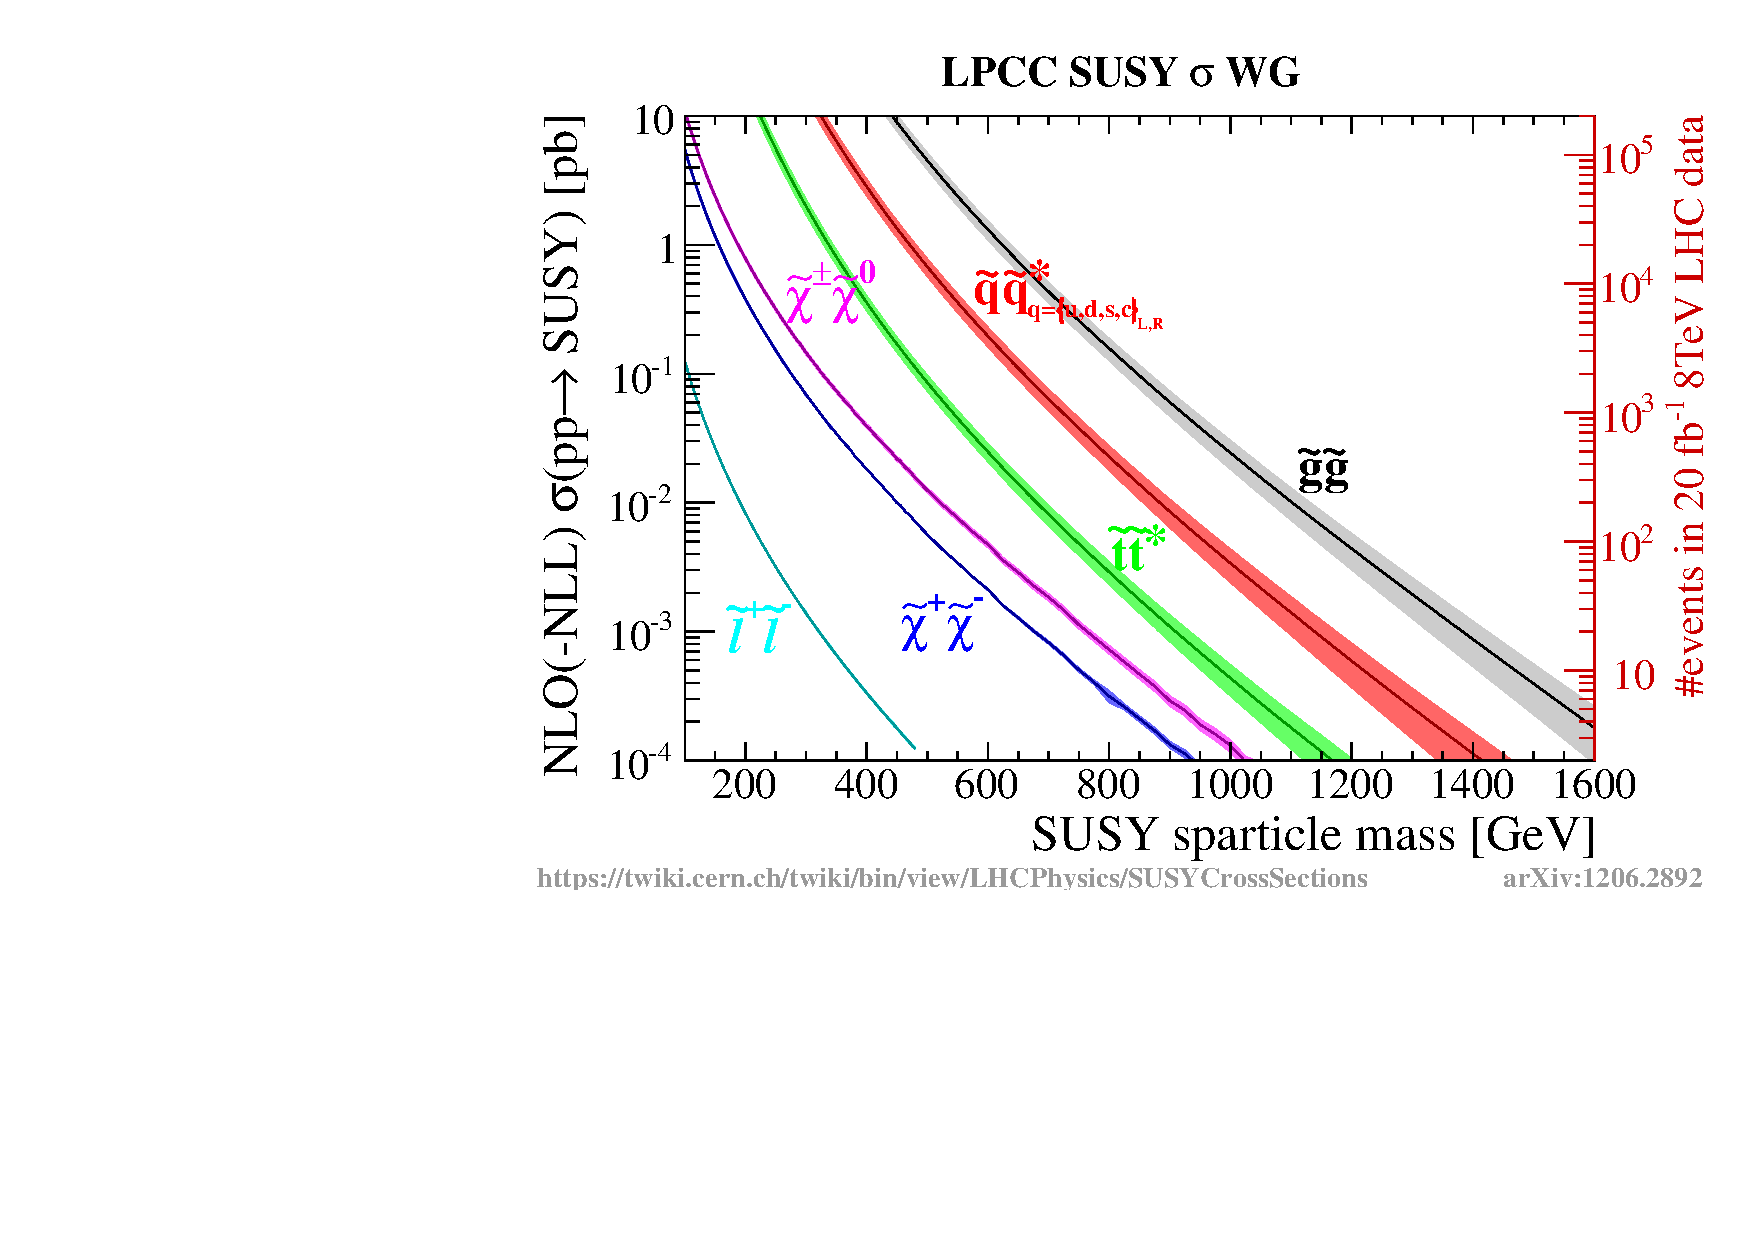
\includegraphics[width=0.8\textwidth]{figures/susy/xsections_strong}
  \caption{Cross sections for the production of various supersymmetric particles at a
centre-of-mass energy of 8\TeV. The expected number of produced events for a dataset of 20\fbinv
are also shown. Figure taken from~\cite{Kramer:2012bx}.
  \label{fig:susy_cross_sections}}
\end{figure}

At the LHC, the production of squarks and gluinos is dominated the gluon-gluon and gluon-quark
fusion. Once produced, they decay as explained in the previous section, possibly resulting in a
long decay cascade in which quarks and leptons can be produced. The full decay chain ends with
the production of at least two LSP's due to the conservation of R-parity. 
When this LSP is a neutralino, it will escape from the detector without being detected. This
will result in an imbalance of transverse momentum, which is one of the most powerful
discriminating variables in the search for SUSY signals. 

In general, SUSY signatures can contain any number of jets, leptons, and gauge bosons, depending on
the details of the mass spectrum. The SUSY search program at the CMS and ATLAS experiments therefore
covers a wide variety of final state topologies. Each analysis will be more or less sensitive to
certain classes of SUSY parameter points, and it is thus of extreme importance to search everywhere,
in all possible ways. The results of these searches can then be interpreted as limits on the
allowed SUSY parameter space. 





\section{Natural SUSY \label{sec:susy_natural_susy}}


Let us now come back to the hierarchy problem. As we have discussed before, radiative corrections
to the Higgs boson mass have the tendency to drive this mass up to very high scales in the SM. When
 supersymmetry is added to the theory, the quadratic contributions disappear due to the symmetries
with the fermions and bosons that run in the loop. However, there are still logarithmic dependencies
on the cutoff scale when SUSY is broken and the masses of the superpartners differ. 
The main contribution to the Higgs mass correction comes from the top quark and top squark loops,
due to the large Yukawa coupling. One can show that the top squark contribution has the general
form,
\begin{equation}
  \Delta m_{H_u}^2 \propto - \frac{3}{8\pi^2} y^2_t \left( m^2_{Q_3} + m^2_{\cPqu_3} + |A_t|^2 
  \right) \log \frac{\Lambda}{1\TeV} .
\end{equation}
Requiring that this term does not become too large, results in a bound on the stop mass of roughly
one \TeV. A similar reasoning can be made for the gluino, which contributes at one-loop level to the
top squark correction, and thus at two-loop level to the Higgs mass correction. The bound for
gluinos to be still considered natural is around 1.5\TeV. 
The $\mu$ parameter also has a big effect on the Higgs boson mass corrections, as it contributes
already at tree-level. The bound on $\mu$, and thus the higgsinos, is of the order of 300\GeV. 

With these considerations in mind, \textit{natural SUSY}~\cite{Barbieri:2009ev,Papucci:2011wy} can
be defined as the subset of the SUSY parameter space for which the above constraints on the
sparticle masses are fulfilled. 
A natural SUSY scenario has low finetuning, and thus resolves the hierarchy problem. A typical mass
spectrum is shown in Fig.~\ref{fig:natural_spectrum}. The idea of natural SUSY has driven many
searches at the LHC, and has drawn particular attention to searches for gluinos and third
generation squarks, as those particles are the only strongly produced particles that are required
to be relatively light. 


\begin{figure}[t]
  \centering
  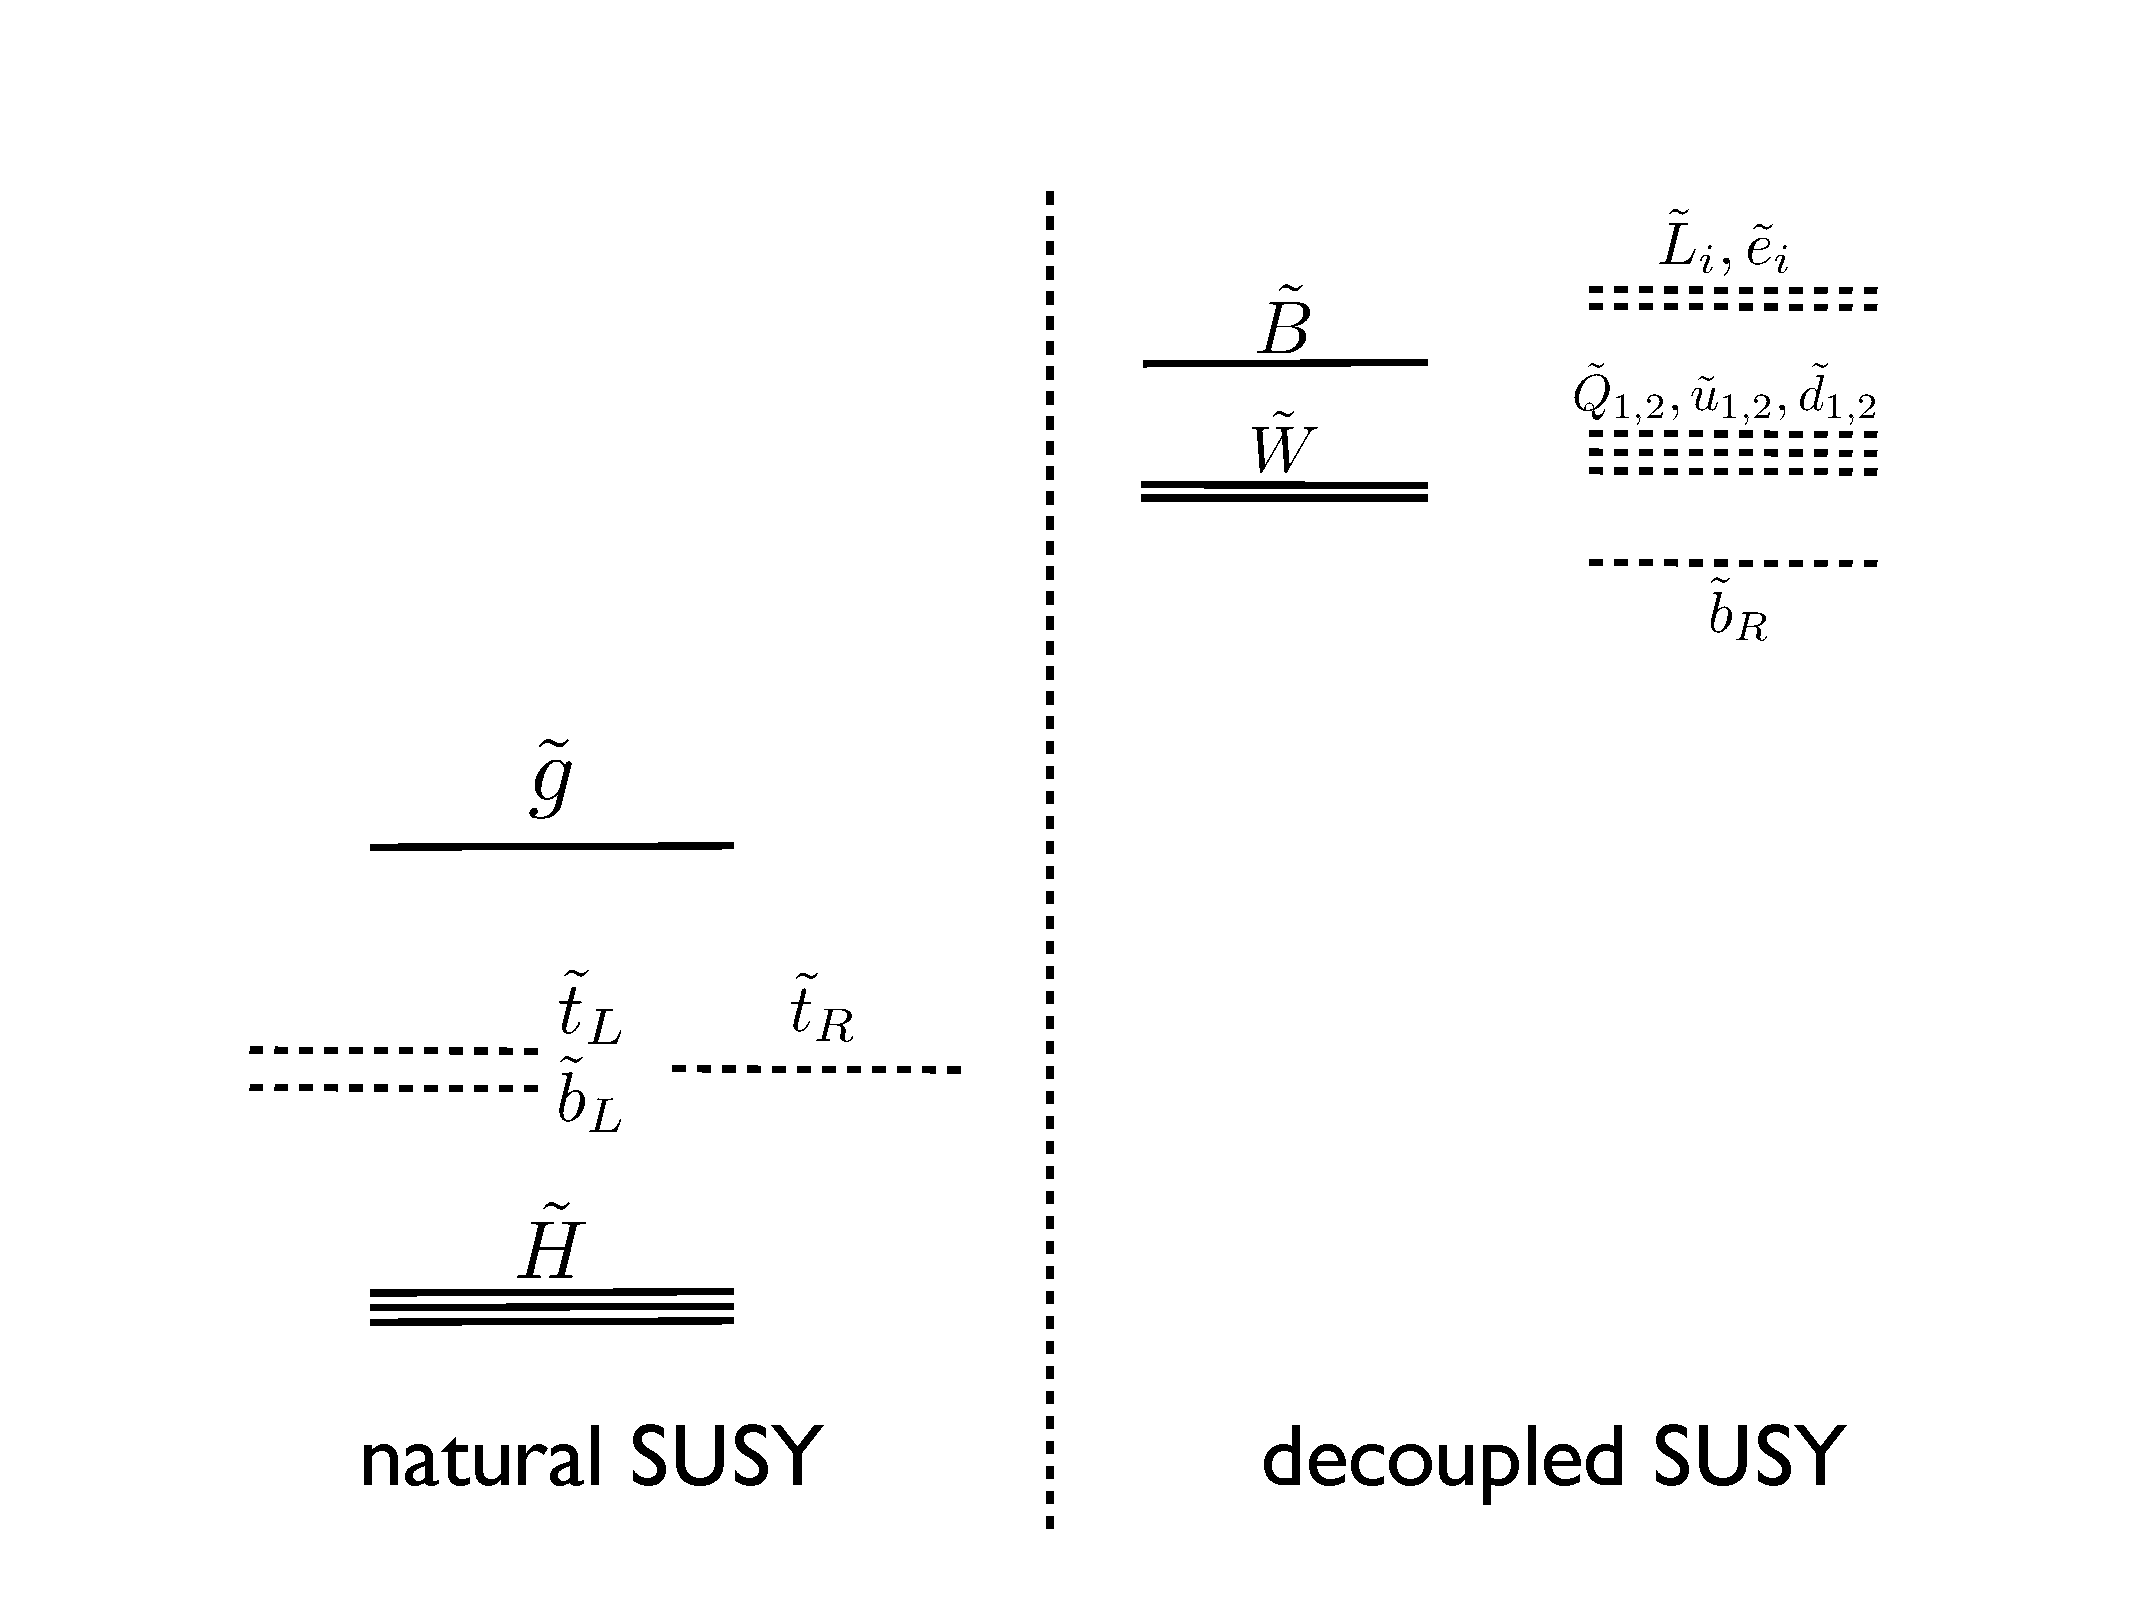
\includegraphics[width=0.8\textwidth]{figures/susy/NaturalSpec}
  \caption{ A natural SUSY spectrum, containing light higgsinos, light top squarks, and a light
gluino. All other superpartners can be decoupled at high masses. Figure taken from
Ref.~\cite{Papucci:2011wy}.
  \label{fig:natural_spectrum}}
\end{figure}


%%%%%%%%%%%%%%%%%%%%%%%%%%%%%%%%%%%%%%%%%%%%%%%%%%%%%%%%%%%%%%%%%%%%%%%%%%%%%%%%%%%%%%%%%%%%%%%%%%%

\section{Simplified model spectra \label{sec:susy_sms}}

Many extensions of the Standard Model are possible, and many of the models have numerous free
parameters. The MSSM is no exception. Without additional simplifications there are 104 extra free
parameters; with a minimal set of assumptions, there are still about 20 parameters left. This
extremely large parameter space is not very practical to do an analysis. 
Furthermore, similar experimental signatures can be produced in different ways, and by different
models.
To address these issues, a simplified approach was developed, using the so-called
\textit{simplified model spectra} (SMS)~\cite{Alves:2011wf,Alwall:2008ag,Chatrchyan:2013sza},
rather than full models. These SMS are based primarily on the experimental topologies, how many jets
or leptons are produced, whether there are jets originating from $\cPqb$ quarks, etcetera. 

Simplified models only contain a limited number of particles and interactions, and can be modelled
as an effective theory. 
The result is a very minimal set of parameters for which no assumptions on relations between
parameters have been made. This makes the simplified models both simpler, and more general.
They are more suitable to optimize and interpret a new physics search compared to a full-fledged
new physics model, for which, depending on assumptions, key topologies could be missing.
The purpose of simplified models is three-fold,
\begin{itemize}
  \item Identifying the boundaries of the search sensitivity. By scanning different masses, or mass
differences between particles, it becomes easier to identify where searches lose sensitivity. This
can then be used as input in the proposal of new dedicated analyses. 

  \item Characterizing possible new physics signals. If a signal is observed, SMS's can be used as
a starting point to quantify the compatibility with different kinds of processes. Starting the
characterization with full models would be very cumbersome due to the many free
parameters that would need to be scanned.

\item Derive limits on more general models. Complex models can be decomposed into experimental
final state topologies. Ideally, each of those topologies would correspond to a SMS. The exclusion
limits on the simplified models can then be translated back into a limit on the full model. 
Several efforts in this respect exist within the phenomenology community, such as
SModelS~\cite{Kraml:2013mwa,Kraml:2014sna}, Fastlim/ATOM~\cite{Papucci:2014rja}, and
checkMATE~\cite{Kim:2015wza}.
\end{itemize}


Let us consider as example a simplified model that only includes a gluino and the lightest
neutralino. We further assume that the gluino can only decay as $\tilde{g}\rightarrow \cPq \cPaq
\lsp$. Simplified models are described by effective theories, in this example the decay
proceeds through the dimension-six operator, 
\begin{equation}
  \mathcal{L}_{\text{int}} = \frac{\lambda_i^2}{M_i^2} \tilde{g} \cPq_i \cPaq_i \lsp + h.c. , 
\end{equation}
where $i$ runs over the different quark flavours, $\lambda_i$ is the Yukawa coupling for the
quark-squark-$\lsp$ vertex, and $M_i$ is the effective scale of the interaction. 
Collision events can be simulated according to this effective Lagrangian in two main ways. The
first is through the use of programs such as \textsc{marmoset}~\cite{ArkaniHamed:2007fw}, which
allows to directly simulate the on-shell effective theory. 
The second, and most widely used, way is to use a matrix element generator, such as \MADGRAPH (see
Section~\ref{sec:event_matrix_element_generators}), to simulate events using the MSSM as model,
setting the masses for all particles that are not involved in the SMS to very high values of
$\mathcal{O}(100\TeV)$.
Any diagrams involving particles not included in the SMS will then effectively not contribute at
all, and the MSSM will be reduced to the SMS under study.  
No matter the details of the simulation, the only parameters that are relevant for this SMS are the
gluino production cross
section, the branching ratio for the decay (here assumed to be 100\%), and the masses for the gluino
and the $\lsp$. Analyses will then usually make a two-dimensional scan across the
($\tilde{g},\lsp$) mass plane, and investigate how their sensitivity changes.


We also note that although the simplified models are SUSY-inspired, and use the SUSY nomenclature,
they are in fact more general. Any model containing a spectrum of new narrow resonances, with the
same gauge and flavour quantum numbers as the SM, and that are odd under some conserved parity, fits
within the scope of the simplified models. Non-SUSY examples are the little Higgs models with
T-parity, or universal extra dimensions with KK-parity. 



 

\section{The Large Hadron Collider \label{chap:LHC}}

The Large Hadron Collider is the world's largest particle accelerator and collider, able to
reach unprecedented particle energies. It is located at CERN, the European Organization for Nuclear
Research on the Swiss-French border near Geneva, in the 27 kilometre long tunnel that previously
housed the Large Electron Positron (LEP) collider. The LHC consists of a sequence of superconducting
magnets that guide two proton beams in opposite directions around the LHC ring, which is composed
of 8 straight and 8 curved sections. 
The beams are accelerated at each turn around the ring, and are made to collide in four interaction
points.
If operating at design conditions, the LHC would provide 600 million $\Pp\Pp$
collisions per second, at a centre-of-mass energy of 14\TeV and a luminosity of
$\text{10}^\text{34}\percms$. 
In the next sections I will highlight some of the main features of the LHC. A more comprehensive
discussion
can be found in Refs.~\cite{Evans:2008zzb,Bruning:2007zzc,Lefevre:1165534,LHC_website}. 

\subsection{A proton machine \label{sec:LHC_proton_machine}}

Both LHC beams contain protons, unlike the previous large accelerators LEP and the Tevatron which
collided electrons on positrons, and protons on antiprotons, respectively. 
The decision to use solely protons was driven by the purpose of the LHC: to be a discovery machine.
The LHC was built to test the Standard Model at unprecedented collision energies, provide
enough data to
probe very rare processes, and hopefully discover new particles. So far the LHC has lived up to
expectation. Per beam energies of up to 4\TeV were reached, providing access to a completely new
energy domain. In 2012 the discovery of the long-sought-after Higgs boson was announced, followed in
2013 by a Nobel prize for Fran\c{c}ois Englert and Peter Higgs, the theorists who first proposed
the existence of this particle. 

The advantage protons have over electrons and positrons is their 2000 times larger mass, resulting
in a much reduced energy loss due to synchrotron radiation. This allows the LHC beam to reach
energies that would be impossible at LEP.
The drawback is the proton's complex structure. Electrons are fundamental particles, which
means that the centre-of-mass energy of the collision is precisely known. This is not the case for
protons. In a $\Pp\Pp$ collision we know the energy of the protons, but not of the individual quarks
and gluons inside the proton that participate in the hard interaction. Consequently, each collision
has a different centre-of-mass energy, making it hard to perform precision measurements. The
compositeness of the protons also leads to messier collisions, as the proton remnants can also
interact and obscure the interesting hard collision event. 

The LHC was built as a $\Pp\Pp$ machine rather than a $\Pp\Pap$ machine because antiprotons are
hard to produce, thus limiting the maximal luminosity that can be achieved. Of course,
there is also a downside here. A proton and antiproton beam can be circulated in opposite
directions using the same magnetic field, and thus beam pipe. However, to steer two proton beams in
opposite direction, we need to apply an opposite magnetic field, meaning that two separate beam
pipes are needed. 

\subsection{LHC accelerator complex and experiments}

% Up to now I have mainly covered what happens to a proton once it enters the LHC ring. In this
% section I will briefly discuss the many steps the protons go through prior to entering the LHC,
% and how they leave it again.

Protons are not simply injected into the LHC itself, but rather pass through a series of
accelerators. 
It all starts with a bottle of hydrogen. Protons are obtained by applying an electromagnetic field
to strip off the electrons from the hydrogen atoms. The protons pass through a linear accelerator,
the Linac 2, where they obtain an energy of 50\MeV, and are then injected into the Proton
Synchrotron (PS) Booster. The booster accelerates the protons to 1.4\GeV at which point the beam is
fed to the PS where it attains an energy of 25\GeV. From the PS the beam is sent to the Super Proton
Synchrotron (SPS) where the protons reach an energy of 450\GeV. 
The beams are then finally transferred to the LHC, both in a clockwise and an anticlockwise
direction, where they are accelerated to their final energy. This entire process is illustrated in
Fig.~\ref{fig:lhc_complex}. 

\begin{figure}[htbp]
  \centering
  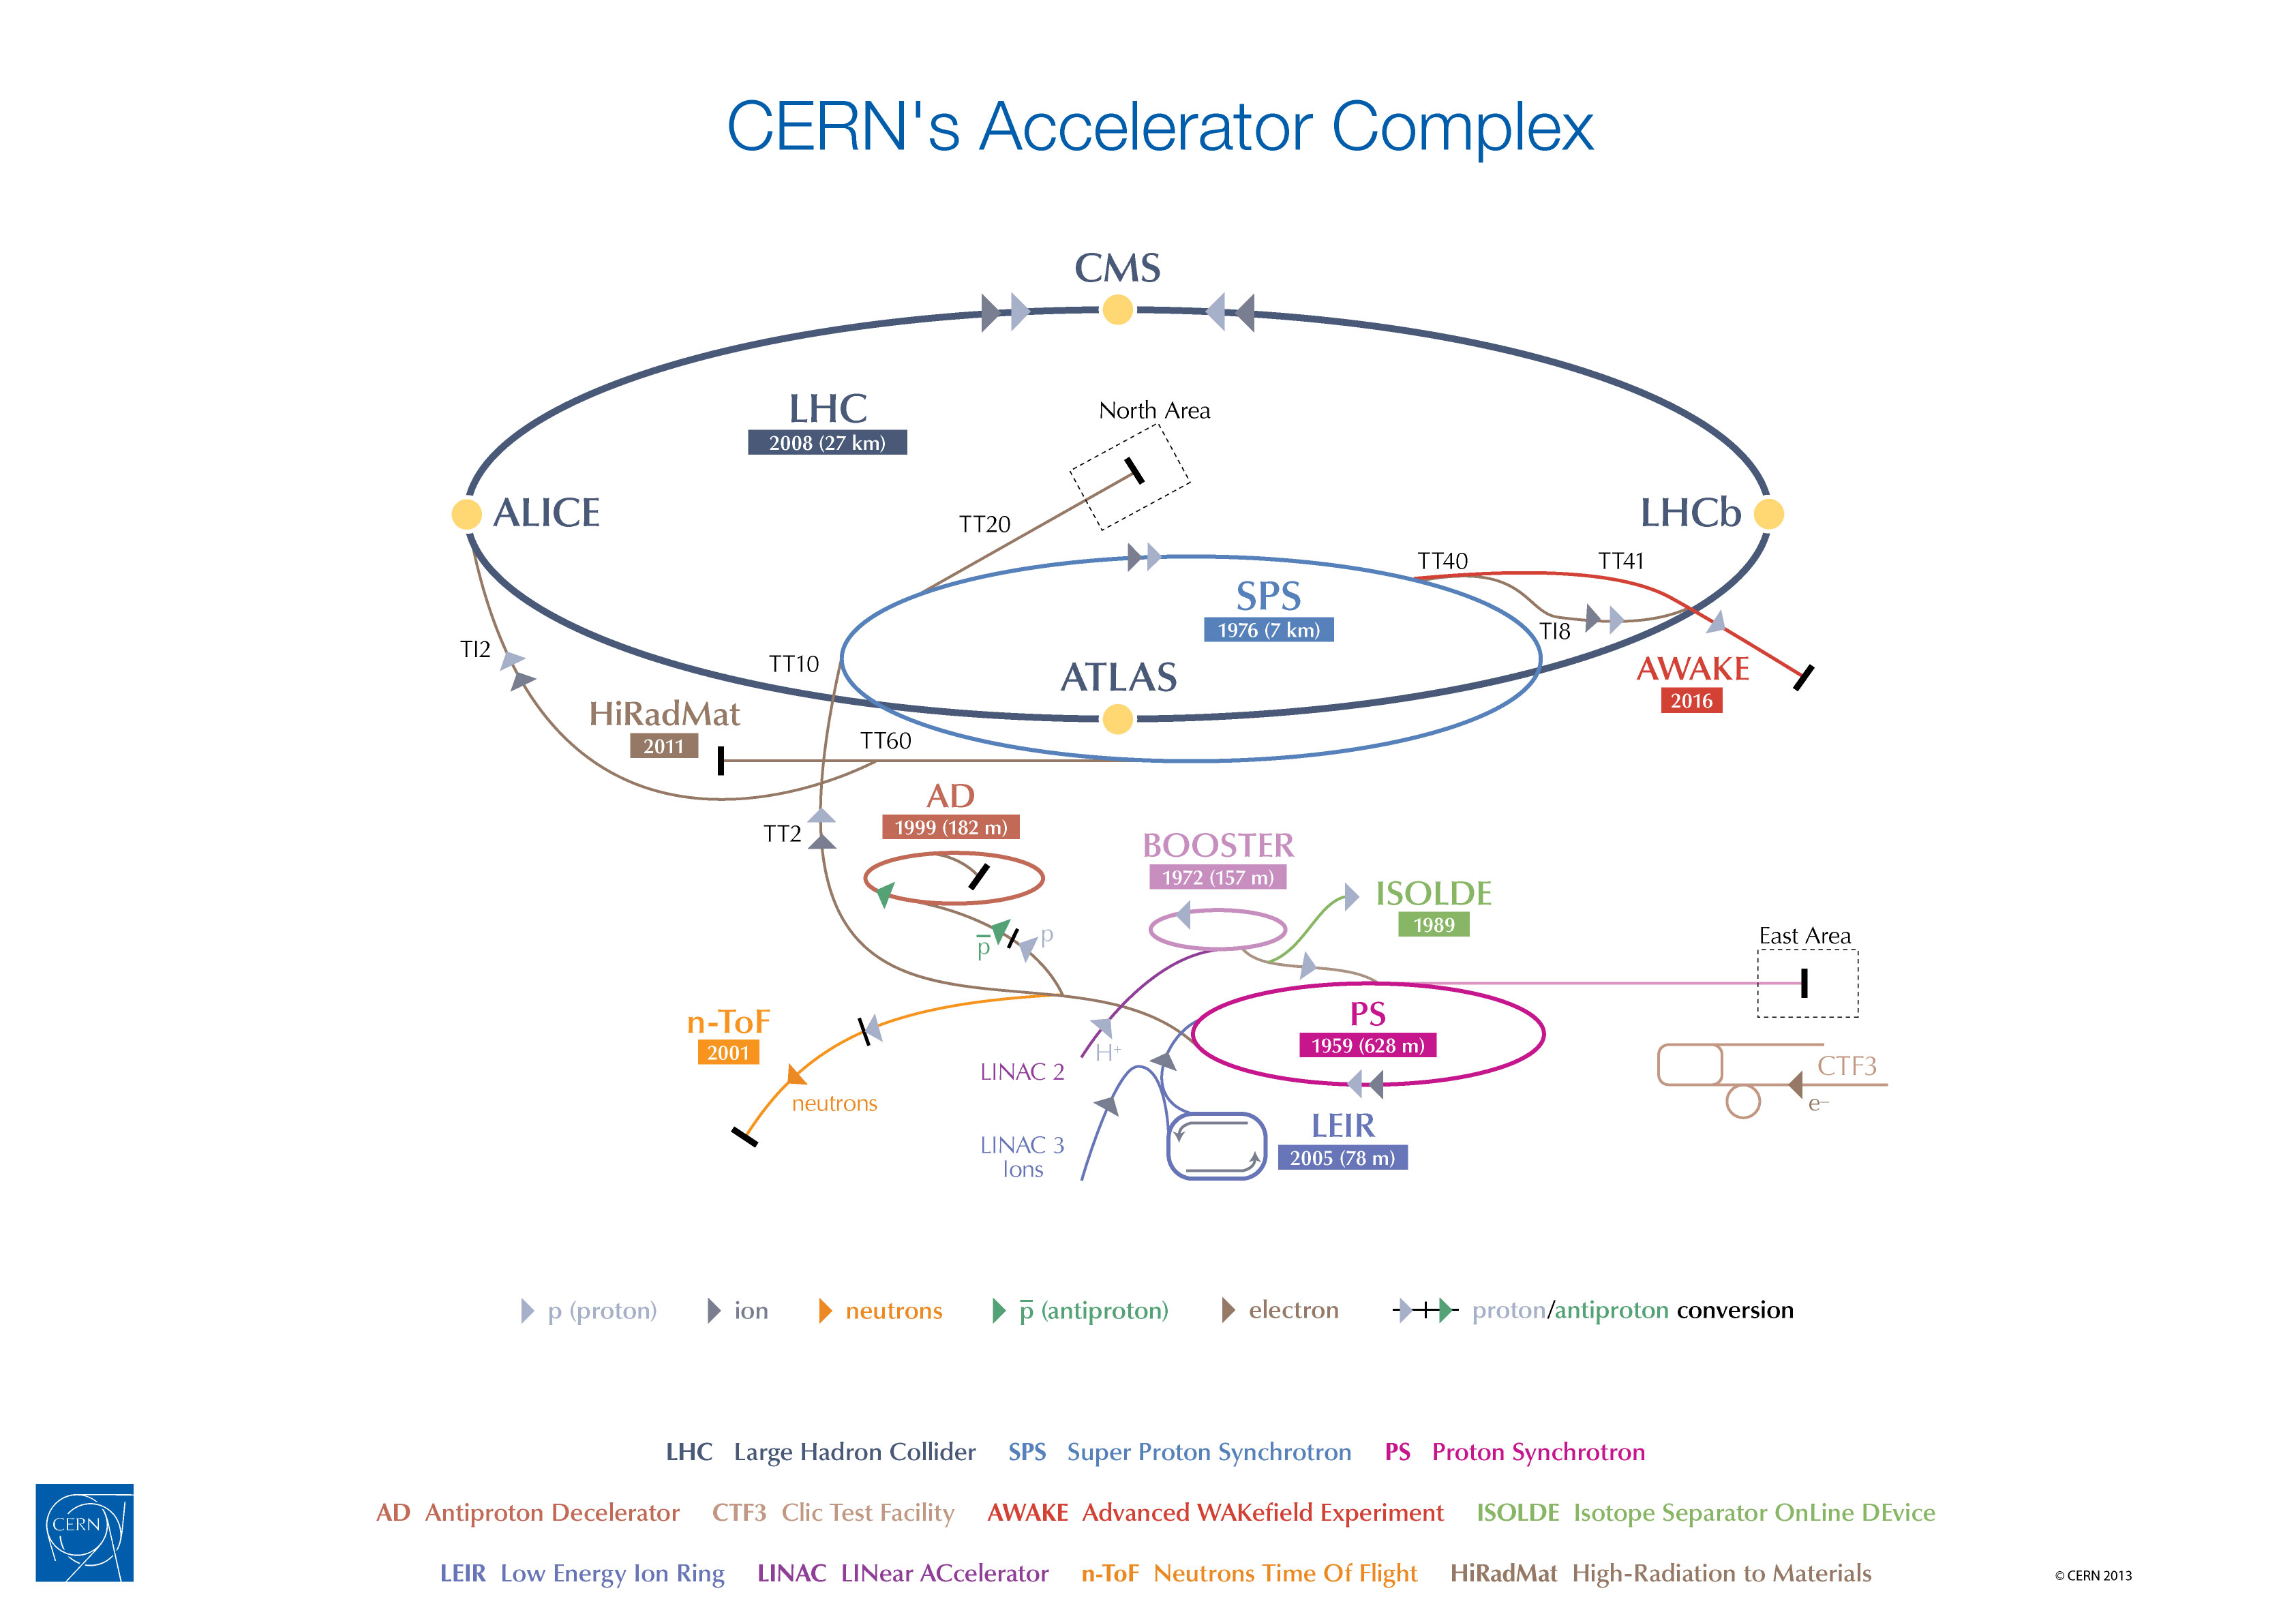
\includegraphics[width=\textwidth,clip=true,trim=10cm 0 13cm 9cm]
  {figures/lhc/cern_accelerator_complex_cds1621583}
  \caption{The CERN accelerator complex. Protons leave the Linac 2, are passed to the Booster, the
PS and SPS, before being injected in the LHC. The four main LHC experiments, CMS, ATLAS, LHCb, and
ALICE, are also shown. Figure taken from Ref.~\cite{lhc_complex}.
  \label{fig:lhc_complex}}
\end{figure}

In addition to accelerating protons, the accelerator complex can also accelerate lead ions, which
are produced from a highly purified lead sample, heated to a temperature of about 500$\de$C. An
electric current is used to ionize the lead vapour.
The lead ions pass through Linac 3, and are then accumulated and accelerated to 72\MeV per nucleon
in the Low Energy Ion Ring (LEIR). 
From the LEIR the ions are transferred to the PS, from where they follow the same path as the
protons, reaching a final energy of 2.76\TeV per nucleon in the LHC. 

Once inserted, beams will circulate inside the LHC beam pipes for many hours under
normal operating conditions. During this time the two beams are made to collide in four interaction
points, each containing a separate detector: 
\begin{itemize}
  \item \textbf{CMS} is a general purpose detector with a very broad physics programme covering
Standard Model measurements, Higgs physics, searches for possible new particles, etcetera. Its
main feature is the huge solenoid magnet, operating at a magnetic field strength of 3.8\unit{T}. The
CMS detector will be explained in more detail in the next chapter. 
  \item \textbf{ATLAS} is a general purpose detector like CMS, with a very similar physics
programme, but utilizing different detector techniques and a magnet design featuring a toroid. At
46\meter long, 25\meter high and 25\meter wide, the ATLAS detector is the largest volume particle
detector ever constructed, although not as heavy as the CMS detector. 
  \item \textbf{LHCb} is a more specialized experiment, aiming to unravel the mysteries of
antimatter by studying processes involving $\cPqb$ quarks. Unlike the cylindrical CMS and ATLAS
detectors, the LHCb detector is asymmetric and targets detection of forward particles in particular.
  \item \textbf{ALICE} is a heavy-ion detector with as primary goal the study of the quark-gluon
plasma, a state of matter occurring at extreme densities. It is the main customer of the LHC
heavy-ion (lead) collision runs.
\end{itemize}
As the two beams collide with each other, or with the remaining gas in the ultrahigh vacuum of
the beam pipe, the beam
intensity keeps dropping. At a certain point more collisions can be delivered to the experiments by
starting the full chain all over again. The beam will then be dumped, and a fresh set of proton
bunches will be inserted. 
If at any time a magnet would \textit{quench}, have an increase in temperature resulting in a loss
of the superconducting state, the beams need to be dumped as well for safety reasons.  

\begin{figure}[tbp]
  \centering
  \begin{tikzpicture}
    \node[anchor=south west, inner sep=0] (image) at (0,0)
{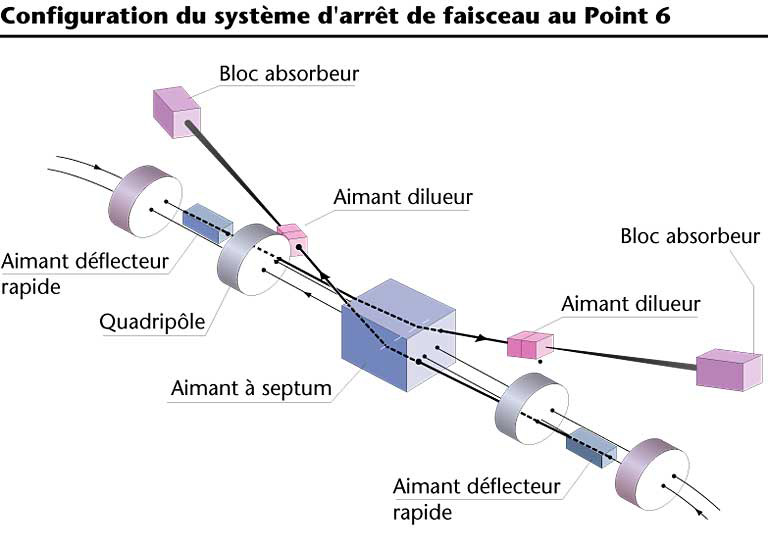
\includegraphics[width=0.8\textwidth,clip=true,trim=0 0 0 2cm]
{figures/lhc/lhc_beamdump_cds842348.jpg}};
    \begin{scope}[x={(image.south east)}, y={(image.north west)}]
      \fill[fill=white] (0.28,0.93) rectangle (0.47,1) node[pos=.5] {\small \textsf{Dump block}};
      \fill[fill=white] (0.43,0.68) rectangle (0.62,0.75) node[pos=.5] {\small \textsf{Dilutor
kicker magnet}};
      \fill[fill=white] (0.8,0.61) rectangle (1,0.67) node[pos=.5] {\small \textsf{Dump block}};
      \fill[fill=white] (0.72,0.465) rectangle (0.93,0.53) node[pos=.45] {\small \textsf{Dilutor
kicker magnet}};
      \fill[fill=white] (0.5,0.05) rectangle (0.74,0.16) node[pos=.45] {\small \textsf{Fast kicker
magnet}};
      \fill[fill=white] (0,0.5) rectangle (0.22,0.62) node[pos=.38] {\small \textsf{Fast kicker
magnet}};
      \fill[fill=white] (0.12,0.42) rectangle (0.28,0.49) node[pos=.45] {\small
\textsf{Quadrupole}};
      \fill[fill=white] (0.22,0.29) rectangle (0.44,0.36) node[pos=.45] {\small \textsf{Septum
magnet}};
     \end{scope}
  \end{tikzpicture}
  \caption{The LHC beam dump system. Figure adapted from Ref.~\cite{lhc_beamdump}.
  \label{fig:lhc_beam_dump}}
\end{figure}

The beam dump system~\cite{Schmidt:2006mi} is shown schematically in Fig.~\ref{fig:lhc_beam_dump}. 
Once the decision to dump the beam is made, a fast kicker magnet is turned on to deflect the beam
in the horizontal plane. 
This kicker magnet has a pulse rise-time of 3\mus. To accommodate this rise-time, and allow for
the safe extraction of the beam, the LHC beam structure is designed to have a gap, where there are
no filled bunches.
The kicker magnets guide the beam onto so-called septum magnets which fully extract the beam from
the beam pipe, deflecting it vertically, and steer it toward the graphite beam dump blocks. The
beam passes through a set of dilutor kicker magnets which spread the beam in both horizontal and
vertical direction, tracing out an `e' shaped path. 
The beam size increases from $0.2\mm$ to $1.5\mm$ upon reaching the dump blocks $700\meter$ away.
Without this dilution, the local beam intensity and heat production would be too large for the
blocks to handle, they would vaporize immediately. However, the graphite core of the dump block
still needs to endure temperatures of up to $750\de$C. The core has a cylindrical shape, 0.7\meter
in diameter and 7.7\meter long, and is surrounded by about 900 tons of radiation shielding blocks.


\subsection{Superconducting magnets}

In order to reach the LHC design centre-of-mass energy of 14\TeV, conventional magnets do not
suffice. Therefore, superconducting magnets are used instead. They can provide the very high
magnetic fields, up to 8.4\unit{T}, needed to bend the highly energetic
particles around the ring, at reasonable power consumption. The magnet coils are built from
niobium-titanium
cable, that when cooled to 1.9\unit{K} attains a superconducting state, allowing electricity to flow
without resistance. The cryostat at the LHC is of unseen proportion, stretching along the
27\unit{km} long ring, and containing 120 tonnes of helium.

The need for two separate beam pipes caused some complication for the LHC design. The LEP tunnel is
quite narrow, too narrow, in fact, to hold two completely separate proton rings. A solution was
found in the so-called twin-bore, or two-in-one, magnet design. This design accommodates the
windings for both beam channels in a common cold mass and cryostat, with the magnetic flux
circulating in the opposite sense through the two channels. 
It also makes the magnet structure more complicated, as the separation between the two channels is
small enough that they are coupled both magnetically and mechanically. An illustration of the
twin-bore design is shown in Fig.~\ref{fig:lhc_twin_bore}. 

Guiding beams around the LHC ring requires thousands of magnets of different varieties and sizes.
Beams are bent by a total of 1232 dipole magnets, each 15 metres in length, and are focussed by 392
quadrupole magnets, each 5–7 metres long. Different kinds of multipole magnets are used to correct
small imperfections in the magnetic field at the ends of the dipoles. So-called insertion magnets
are used to squeeze the beam from 0.2 millimetres down to 16 micrometres across, just before it
reaches one of the detectors in the interaction points. 

\begin{figure}[t]
  \centering
  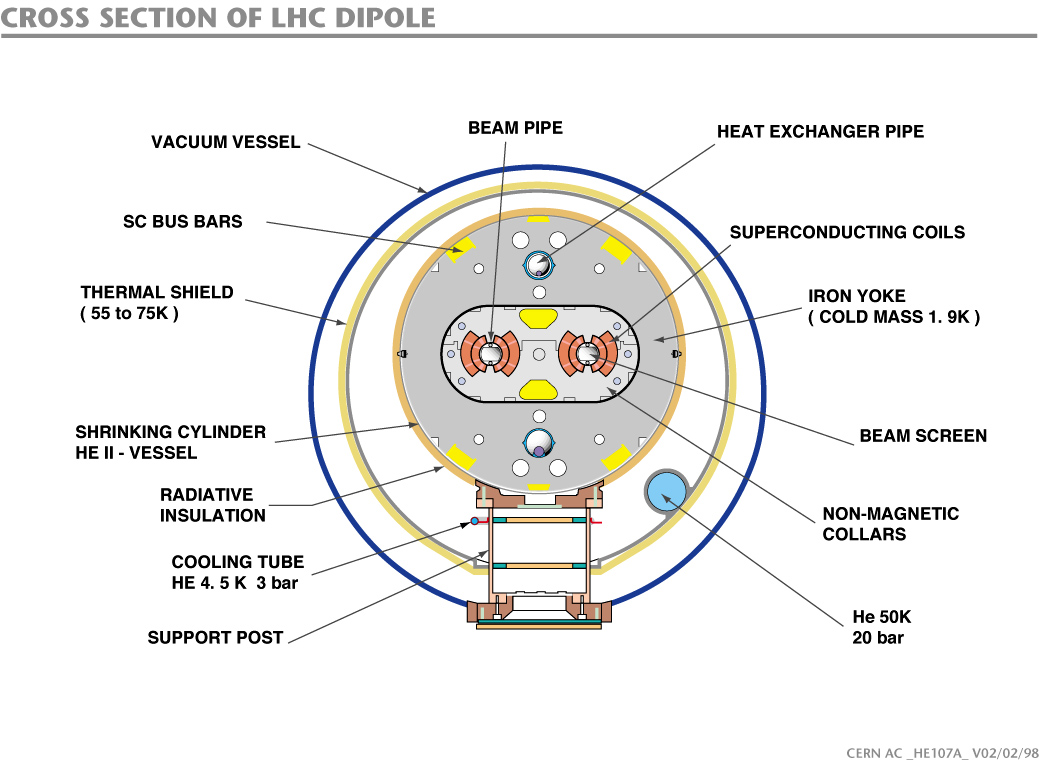
\includegraphics[width=\textwidth,clip=true,trim=0 2cm 0 2cm]
  {figures/lhc/lhc_dipole_cross_section_cds841539.jpg} 
  \caption{Cross section of an LHC dipole magnet, illustrating the twin-bore magnet
design~\cite{cds:841539}. The two beam pipes surrounded by the dipole magnets are clearly
visible. They are encased in a single cold volume and vacuum vessel. 
  \label{fig:lhc_twin_bore}}
\end{figure}


\subsection{Accelerating cavities}

The necessary accelerating power to raise the beam energy from the injection energy of 450\GeV to
the collision energy of several \TeV is provided by eight radiofrequency (RF) cavities per beam. 

RF cavities are metal chambers, often structured like beads on a string, where the beads are the
cavities and the string is the beam pipe of the accelerator.
An electromagnetic (EM) field is supplied to the cavities by an RF power generator. The specific
shape and size of the cavities are such that the EM waves become resonant, and build up inside the
cavity. 
Charged particles passing through the cavity feel the force and direction of the resulting
electromagnetic field, and are pulled along with the field. 
As the field in the LHC RF cavities oscillates at 400\unit{MHz}, the arrival of the protons needs to
be timed precisely in order for them to be accelerated, and not decelerated, see 
Fig.~\ref{fig:RF_explanation}. 
Once the particles have circled the LHC ring a sufficient number of times, passing through
the RF cavities on each turn, they attain the desired energy. At this point the main purpose of the
RF cavities is to keep the protons inside their \textit{bunches}. 

\begin{figure}[tpb]
  \centering
  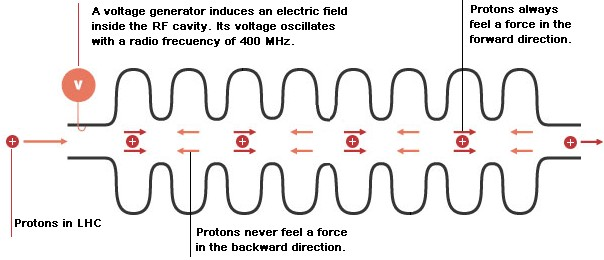
\includegraphics[width=0.8\textwidth]{figures/lhc/RF_explanation}
  \caption{Interaction between a proton and the oscillating electromagnetic field inside a
radiofrequency cavity. Figure taken from Ref.~\cite{RF_explanation}.
  \label{fig:RF_explanation}}
\end{figure}

The protons in the LHC beams do not form a continuous flow, but are grouped in packets, the bunches,
with empty space in between. Up to 2808 bunches can circle the LHC at any
given time. An ideally timed proton, with exactly the right energy, will see zero
accelerating voltage from the RF cavities when the LHC is at full energy. Protons with slightly
different energies arriving earlier or later will be accelerated or decelerated so that they stay
close to the energy of the ideal particle. In this way, the beam bunches stay intact. 

The LHC utilizes superconducting RF cavities made of niobium sputtered on copper, which are
cooled to 4.5\unit{K}. The RF power, up to 2\unit{MV} per cavity, is delivered by klystrons and
passed to the cavities via waveguides. Protons can thus gain up to 16\MeV per turn around the ring.
The RF cavities are grouped by fours in cryomodules, which are installed in a straight section of
the LHC tunnel. 



\subsection{Past and future running periods}

The first proton beams circled the LHC in September 2008. Unfortunately, an incident happened
shortly thereafter, during powering tests of the dipole magnet. A faulty connection caused  an
electrical
arc which punctured the helium enclosure, leading to a release of helium into the insulation vacuum
of
the cryostat. The pressure from the expanding helium rose too fast for the relief valves to cope,
thereby damaging dozens of magnets. It took more than one year to repair all the damage, and
install extra safety systems. 

In November 2009 beams were back in the LHC, with first stable beams
at 7\TeV centre-of-mass energy in March 2010. The LHC continued to run very smoothly throughout
2011, delivering data corresponding to an integrated luminosity of 5\fbinv to the experiments.  
In 2012 the beam energy was increased from 3.5 to 4\TeV, and also the luminosity of the beam saw a
sharp increase. A total integrated luminosity of over 20\fbinv was delivered. 

During 2013 and 2014 the LHC was shut down for maintenance and upgrade, in order to prepare the
machine to run at 13\TeV centre-of-mass energy and higher instantaneous luminosity. During these two
years, the experiments at the interaction points were also upgraded to increase detector performance
in light of the changing conditions expected upon restart. 
First stable beams for physics collisions at 13\TeV are planned for June 2015. This will signal the
start of a very exciting time for particle physics, during which our understanding of elementary
particles and their interactions will undoubtedly change. 




\chapter{The Compact Muon Solenoid experiment \label{chap:CMS}}

The Compact Muon Solenoid (CMS)~\cite{Chatrchyan:2008aa,Bayatian:922757,Ball:2007zza,CMS_website} is
one of the two general purpose detectors
at the LHC. It is
located on the far-end of the LHC ring, at interaction point 5 (P5) in Cessy, France. 
Like most collider experiments, CMS has a cylindrical shape, consisting of a barrel region and two
so-called endcaps at either end of the barrel. The various subdetector systems are layered around
the collision point. The central feature of the CMS detector is the superconducting solenoid with
high magnetic field to achieve good momentum resolution. The muon systems are installed in between
the return yoke layers. The silicon tracker, lead-tungstate crystal electromagnetic calorimeter
(ECAL), and brass scintillator hadron calorimeter (HCAL) are contained within the bore of the magnet
coil. 
The CMS detector has a length of 21\meter, a diameter of 15\meter and a total weight of $14\,000$
tonnes. 
Figure~\ref{fig:cms_overview} shows an overview of the detector and its different
subsystems. It is important to note that different kinds of particles interact differently with the
various subdetectors, as illustrated in Fig.~\ref{fig:cms_slice}. This design allows the
reconstruction software to distinguish between electrons, muons, photons, charged and neutral
hadrons. 
A more extensive discussion on each subsystem will be given in the
following sections. 

\begin{figure}[htpb]
  \centering
  \includegraphics[width=0.9\textwidth]{figures/cms/CMS_overview_labelled}
  \caption{Overview of the CMS detector. The different subsystems are indicated on the figure, as
well as a person to serve as reference scale. Figure taken from Ref. \cite{CMS_overview_labelled}.
  \label{fig:cms_overview}}
\end{figure}

\begin{figure}[htpb]
  \centering
  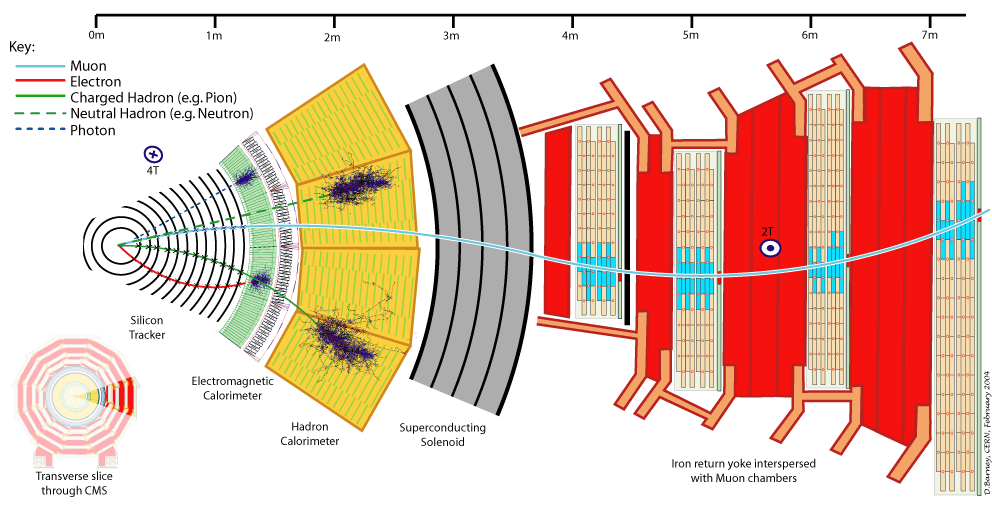
\includegraphics[width=0.9\textwidth]{figures/cms/CMS_Slice}
  \caption{Detailed view of a CMS detector slice, showing the interactions of different kinds of
particles with the various subsystems. Muons leave hits in the tracker and the muon stations,
before leaving the detector. Electrons leave hits in the tracker, and then deposit their
energy in the ECAL. Photons can be identified as an energy deposit in the ECAL without a
corresponding track. Charged and neutral hadrons both deposit their energy in the HCAL, with
matching tracker hits for charged hadrons only. 
Figure taken from Ref.~\cite{CMS_slice}.
  \label{fig:cms_slice}}
\end{figure}

%%%%%%%%%%%%%%%%%%%%%%%%%%%%%%%%%%%%%%%%%%%%%%%%%%%%%%%%%%%%%%%%%%%%%%%%%%%%%%%%%%%%%%%%%%%%%%%%%%%%
\section{Coordinate system and basic variables \label{sec:cms_coordinates}}

The CMS coordinate system takes the nominal collision point as the origin, with the $y$-axis
pointing vertically upward, and the $x$-axis pointing radially inward towards the center of the
LHC. The coordinate system is right-handed, such that the $z$-axis points along the beam direction
toward the Jura mountains as seen from P5. 
The azimuthal angle $\phi$ is measured from the $x$-axis in the ($x,y$) plane. The polar angle
$\theta$ is measured from the $z$-axis. 
Pseudorapidity $\eta$ is defined as 
\begin{equation}
 \eta = - \ln \left[ \tan(\theta/2) \right],  
\end{equation}
and is usually used instead of the
polar angle because of the property that differences in pseudorapidity are
Lorentz-invariant. This is especially useful for hadron colliders where the boost in the $z$
direction is unknown, and varies for each collision. A Lorentz-invariant angular separation between
two particles is defined as 
\begin{equation}
\Delta R = \sqrt{(\Delta\eta)^2 + (\Delta\phi)^2}.
\end{equation}
The momentum and energy measured transverse to the beam direction, denoted by $\pt$ and $\ET$,
respectively, are computed from the $x$ and $y$ components.
The imbalance of energy measured in the transverse plane is denoted by \ETm, and indicates
undetected particles, or energy mismeasurements.
 

% 1.3.1 Summary of detector requirements
% The detector requirements for CMS to meet the goals of the LHC physics programme can be
% summarized as follows:
% • Good muon identification and momentum resolution over a wide range of momenta
% in the region |η| < 2.5, good dimuon mass resolution (≈ 1% at 100 GeV/c2),
% and the ability to determine unambiguously the charge of muons with p < 1 TeV/c.
% • Good charged particle momentum resolution and reconstruction efficiency in the
% inner tracker. Efficient triggering and offline tagging of τ ’s and b-jets, requiring1.4.
% Experimental challenge 7
% pixel detectors close to the interaction region.
% • Good electromagnetic energy resolution, good diphoton and dielectron mass resolution
% (≈ 1% at 100 GeV/c2), wide geometric coverage (|η| < 2.5), measurement
% of the direction of photons and/or correct localization of the primary interaction
% vertex, π0 rejection and efficient photon and lepton isolation at high luminosities.
% • Good Emiss
% T and dijet mass resolution, requiring hadron calorimeters with a large
% hermetic geometric coverage (|η| < 5) and with fine lateral segmentation (∆η ×
% ∆φ < 0.1 × 0.1).
% The design of CMS, detailed in Section 1.5, meets these requirements. The main distinguishing
% features of CMS are a high-field solenoid, a full silicon-based inner tracking system, and
% a fully active scintillating crystals-based electromagnetic calorimeter.

%%%%%%%%%%%%%%%%%%%%%%%%%%%%%%%%%%%%%%%%%%%%%%%%%%%%%%%%%%%%%%%%%%%%%%%%%%%%%%%%%%%%%%%%%%%%%%%%%%%%
\section{Magnet system \label{sec:cms_magnet}}

The CMS magnet is a superconducting solenoid, producing a uniform magnetic field of 3.8\unit{T}
inside the magnet coil. 
Having a magnet is key to the success of any collider experiment. Without the bending of charged
particle tracks in the magnetic field, it would be very hard, if not impossible, to obtain
accurate momentum and charge measurements for those particles. 
Since the curvature decreases as the \pt of the particles increases, the strength of the magnetic
field, and the precision of the tracker, will determine how accurately the momentum of highly
energetic particles can be measured. 

To take as much advantage of track bending as possible, CMS decided they wanted to have the
strongest magnetic field possible. Therefore, the largest magnet that could be transported to P5
was built. The CMS solenoid measures 6.3\meter in diameter, and the steel return yoke has an outer
diameter of 14\meter. The total magnet system is 13\meter long, weighs a whopping $12\,000$ tonnes,
and is the largest superconducting magnet ever built. The solenoid is cooled to 4.5\unit{K}, and the
very strong magnetic field of 3.8\unit{T} results in a momentum resolution of $\Delta p / p \approx
10\%$ at momenta of 1\TeV, sufficient to determine the sign of muons with $\pt \approx 1 \TeV$. 

The tracker, ECAL, and HCAL fit inside the magnet coil, whereas the muon stations are interleaved
with the return yoke. The yoke is made up of three layers, as shown in Fig.~\ref{fig:cms_magnet},
provides most of the structural support for the whole experiment, and acts as a shield that blocks
any particles that made their way across the HCAL, apart from muons, neutrinos, and possible new
weakly interacting particles. 

\begin{figure}[htpb]
  \centering
  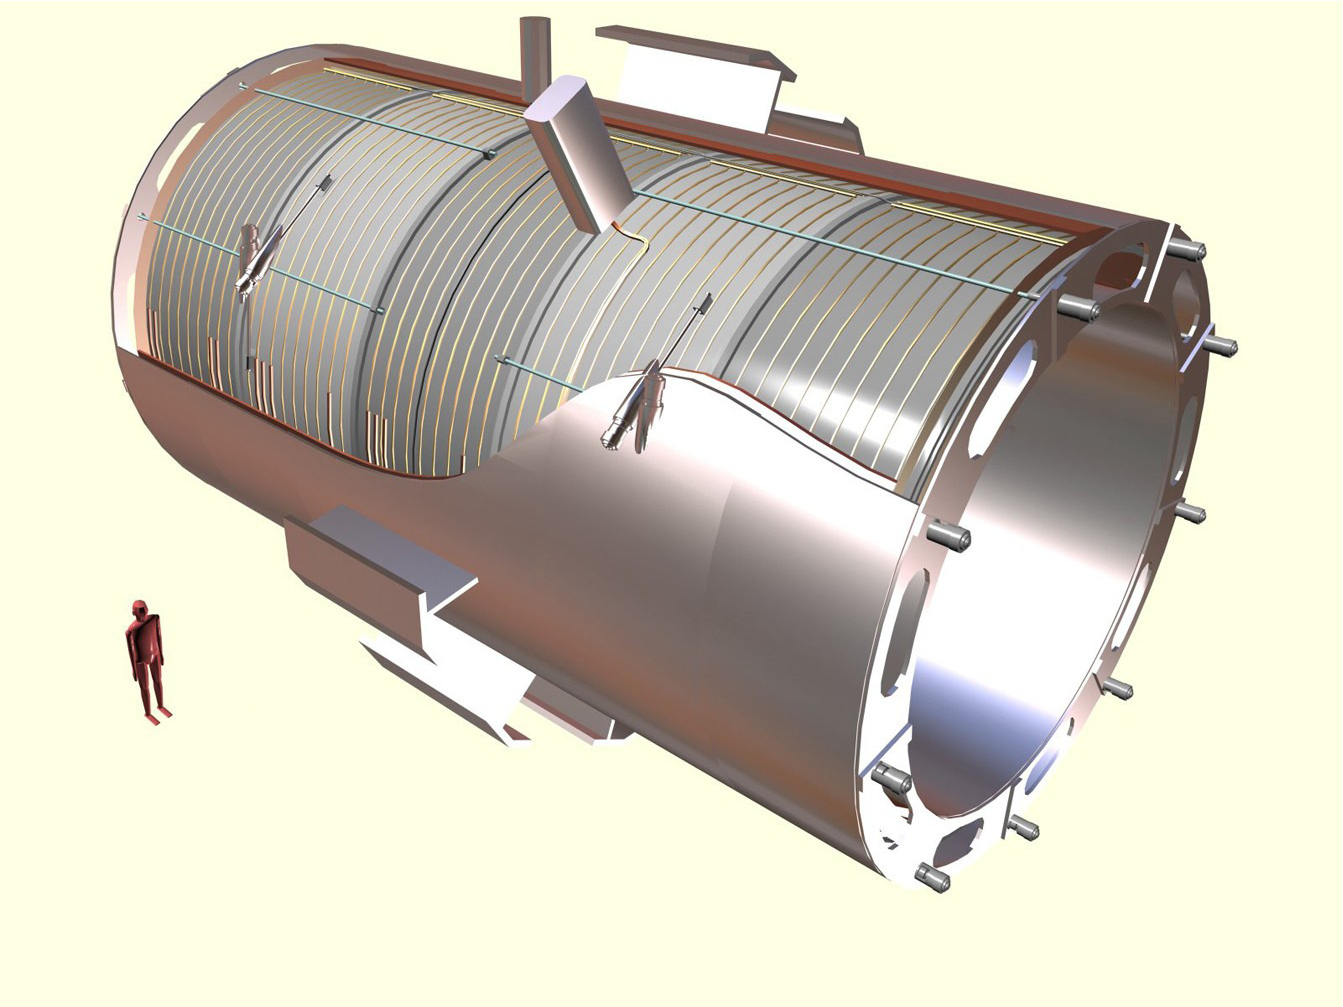
\includegraphics[height=0.2\textheight,clip=true,trim=0 2cm 0 0]{figures/cms/CMS_solenoid}
  ~
  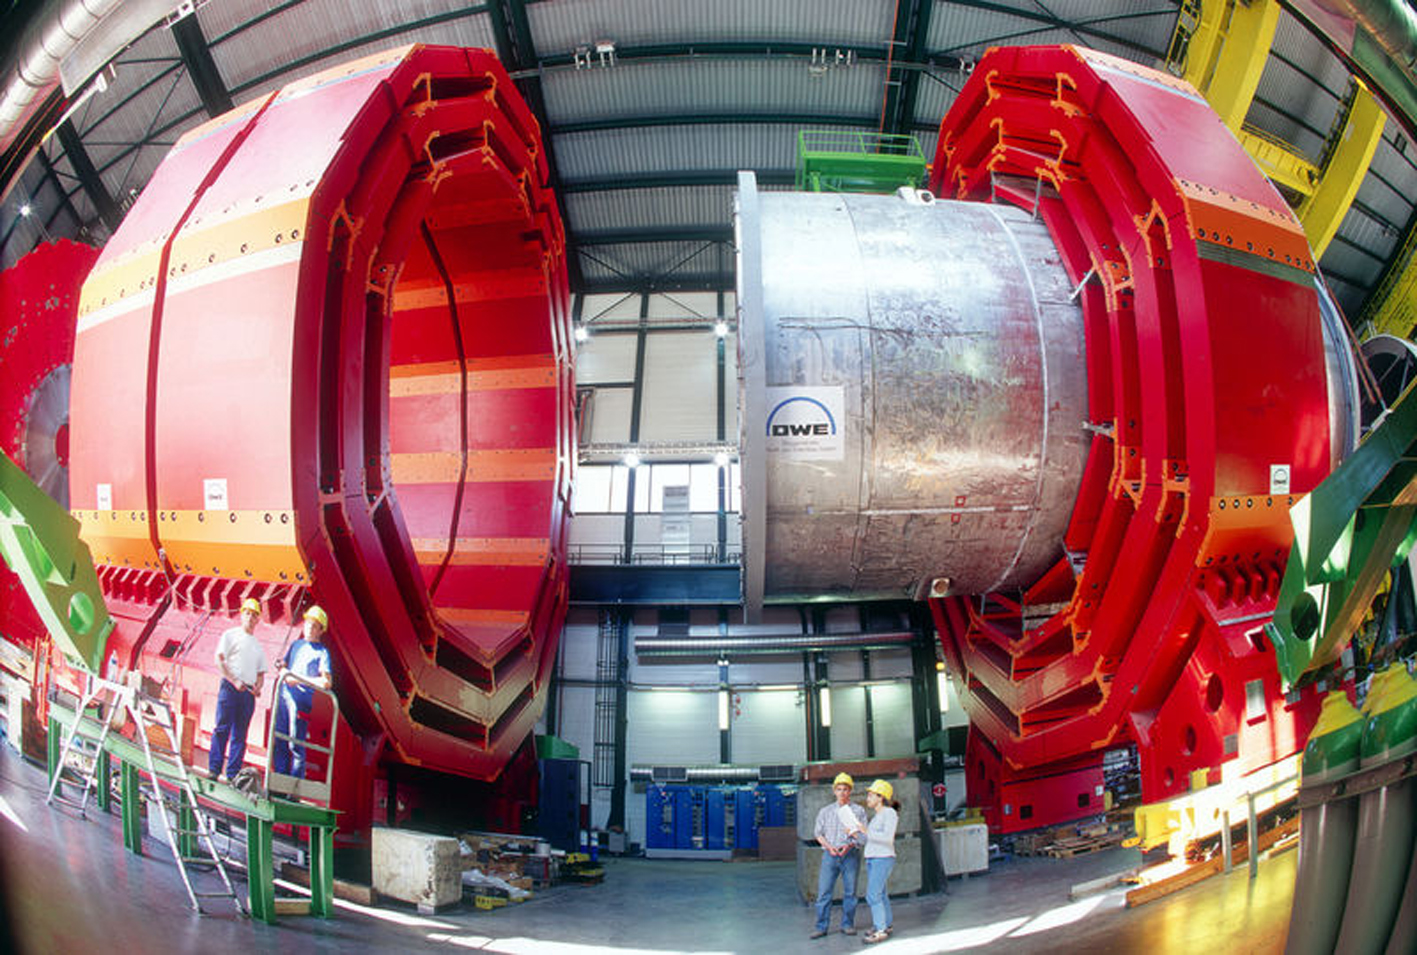
\includegraphics[height=0.2\textheight]{figures/cms/cms_magnet}
  \caption{[left] Artistic view of the superconducting solenoid showing the five modules composing
the cold mass inside the cryostat. Figure taken from Ref.~\cite{Chatrchyan:2008aa}.
  [right] Fish-eye view of the red magnet yoke during construction in
2002. Figure taken from Ref.~\cite{CMS_magnet}.
  \label{fig:cms_magnet}}
\end{figure}

%%%%%%%%%%%%%%%%%%%%%%%%%%%%%%%%%%%%%%%%%%%%%%%%%%%%%%%%%%%%%%%%%%%%%%%%%%%%%%%%%%%%%%%%%%%%%%%%%%%%
\section{Tracker \label{sec:cms_tracker}}

The purpose of the tracker is to very accurately measure the curved tracks of charged
particles with $\pt > 1\GeV$, such that a precise momentum measurement can be made. 
The tracker should also be able to precisely reconstruct secondary
vertices stemming from e.g. $\cPqb$ quark decays. 
In addition, particles should be disturbed the least amount possible while passing through the
tracker. The tracker should thus consist of as little material as possible in order to avoid
multiple scattering, bremsstrahlung, photon conversion, and nuclear interactions.
To accomplish this, the tracker consists of several thin layers. When a particle passes
through a layer, it creates a signal, a \textit{hit}. Out of the different hits, the reconstruction
software then builds a track. 

The tracker is the innermost layer of the CMS detector, perfectly placed to measure the particles
coming directly from the collision point. Its closeness to the beam pipe also means that it will
receive the largest amount of particles, and thus radiation, which translates into the need for
radiation hard materials. 

The CMS tracker is entirely built out of silicon, and consists of a pixel detector at the very
center, surrounded by a microstrip detector. It has a length of 5.8\meter and a diameter of
2.5\meter. With about 200$\meter^\text{2}$ of active silicon area, the CMS tracker is the largest
silicon tracker ever built. A diagram of the structure is shown in
Fig.~\ref{fig:cms_tracker}, alongside a photograph of part of the strip detector. 
There are a total of 75 million read-out channels with very fast response, providing a precision of
10\mum in position measurement, even when up to 1000 particles traverse the tracker every
25\unit{ns}. This corresponds to a transverse momentum resolution of 1-2\% for $\pt \approx
100\GeV$. 

The pixel detector has three cylindrical layers very close to the collision point (at 4\cm, 7\cm and
11\cm from the beampipe), and two disks at either end. Each of the 65 million pixel sensors measures
100\mum by 150\mum. A cooling system is installed to keep the temperature from rising too much. The
operating temperature is $-10\de$C.

The silicon strip detector consists of ten layers in total. There are four inner barrel (TIB)
layers with two inner endcaps (TID), each composed of three small discs. The outer barrel (TOB)
consists of six layers, while two endcaps (TEC) close off the tracker. The strip tracker is
cooled to a temperature of $-20\de$C in order to minimize the spreading of any radiation
damage.

\begin{figure}[tpb]
  \centering
  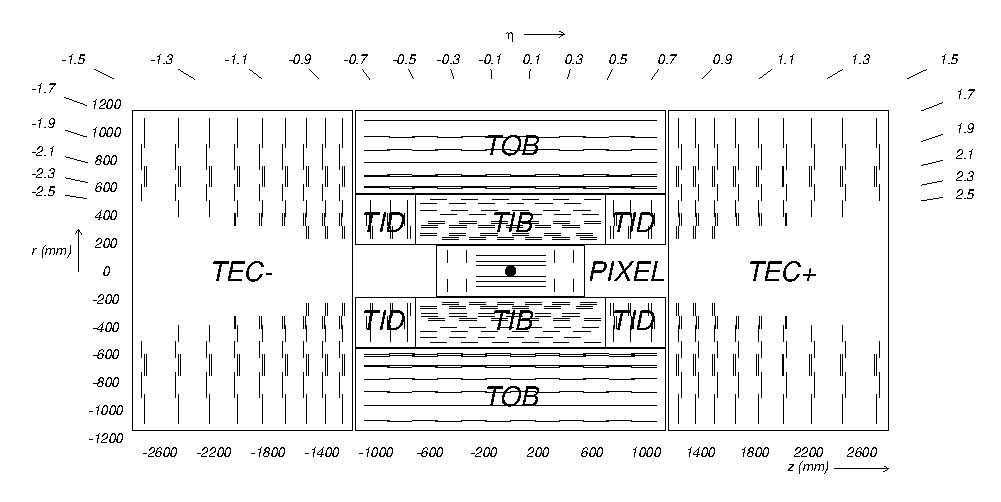
\includegraphics[height=0.17\textheight]{figures/cms/CMS_tracker_general_layout}
  ~
  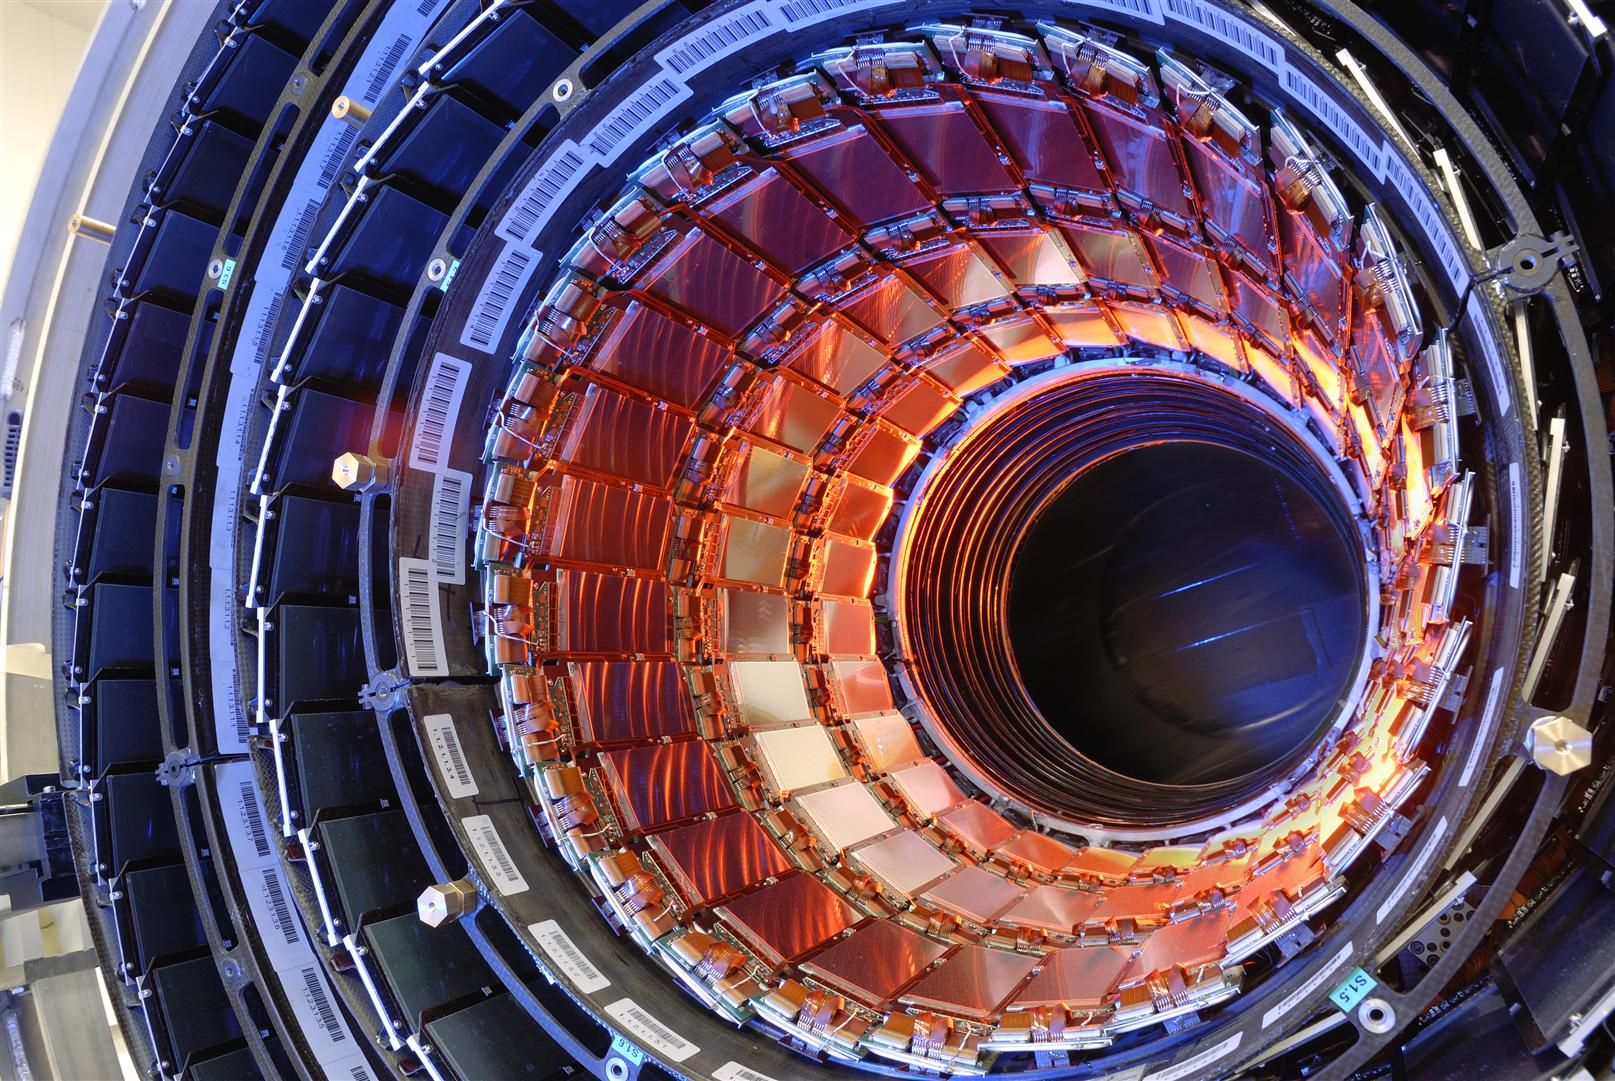
\includegraphics[height=0.17\textheight]{figures/cms/cms_tracker}
  \caption{[left] Schematic cross section through the CMS tracker. Each line represents a detector
module. Figure taken from Ref.~\cite{Chatrchyan:2008aa}. 
  [right] The first half of the CMS inner tracker barrel (TIB), consisting of three
layers of silicon modules. Figure taken from Ref.~\cite{CMS_tracker}.
  \label{fig:cms_tracker}}
\end{figure}

%%%%%%%%%%%%%%%%%%%%%%%%%%%%%%%%%%%%%%%%%%%%%%%%%%%%%%%%%%%%%%%%%%%%%%%%%%%%%%%%%%%%%%%%%%%%%%%%%%%%
\section{Electromagnetic calorimeter \label{sec:cms_ecal}}

The CMS electromagnetic calorimeter is a hermetic homogeneous calorimeter, consisting of a central
barrel region and two endcaps, and is located in between the tracker and the HCAL. 
It has a fine granularity, is fast, and is radiation resistant.
The ECAL provides a very good energy resolution for electrons and photons, which played a key role
in the discovery of the Higgs boson in the $h\rightarrow\gamma\gamma$ final state. 

The ECAL is made of about $75\,000$ highly transparent lead tungstate ($\text{PbWO}_\text{4}$)
crystals whose length corresponds to about 25 radiation lengths. A photograph of the crystals
during testing, and a schematic view of the ECAL structure is shown in
Fig.~\ref{fig:cms_ecal_crystal}. The crystals are arranged side-by-side with their longitudinal axes
slightly pointed away from the interaction point to avoid cracks.

When electrons or photons pass through such a lead tungstate crystal, it scintillates. 
This scintillation light is detected, and converted to an electrical signal, by avalanche
photodiodes (APDs) in the barrel, and vacuum phototriodes (VPTs) in the endcaps.
The scintillation decay time is very short, about 80\% of the light is emitted within 25\unit{ns},
which is ideal for the bunch spacing of the LHC. 
The light yield of the crystals depends strongly on temperature, however. In order to keep the
temperature at a stable level, to within 0.1\de C, a dedicated temperature control system was put in
place.
Even though the crystals are quite radiation hard, they still suffer damage in the very high
particle flux environment within CMS. Fortunately, the damage repairs itself through annealing
during the periods when the accelerator is not operational, and the temperature of the crystals is
higher. A light monitoring system is used to accurately measure the transparency of the crystals
throughout the running period, so that precise energy measurements can always be made. 

Preshower detectors in front of the ECAL endcaps provide for extra spatial precision, making it
possible to distinguish between single high-energy photons and the less interesting close pairs of
low-energy photons coming from the decay of neutral pions.
The preshower detector is a sampling calorimeter, consisting of two planes of lead radiators that
initiate showers when an electron of photon passes through. Behind each lead plane are sensors that
measure the deposited energy and transverse shower profiles. 
The sensors are silicon strip detectors of only 2\mm wide, compared to 3\cm for the ECAL endcap
crystals. The two layers of strips are placed orthogonally, thus providing a position
measurement with extremely fine granularity. 


\begin{figure}[htpb]
  \centering
  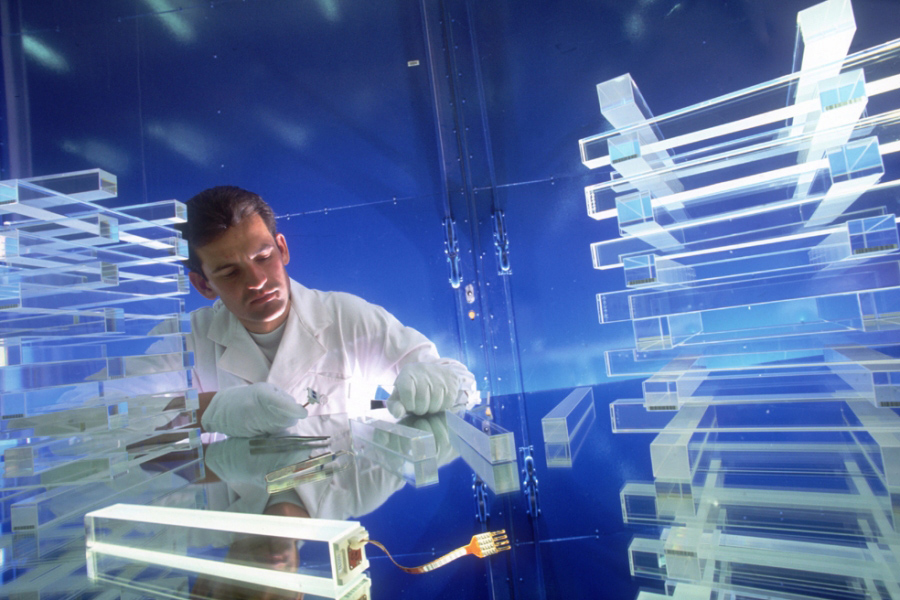
\includegraphics[width=0.48\textwidth]{figures/cms/cms_ecal_crystal}
~
  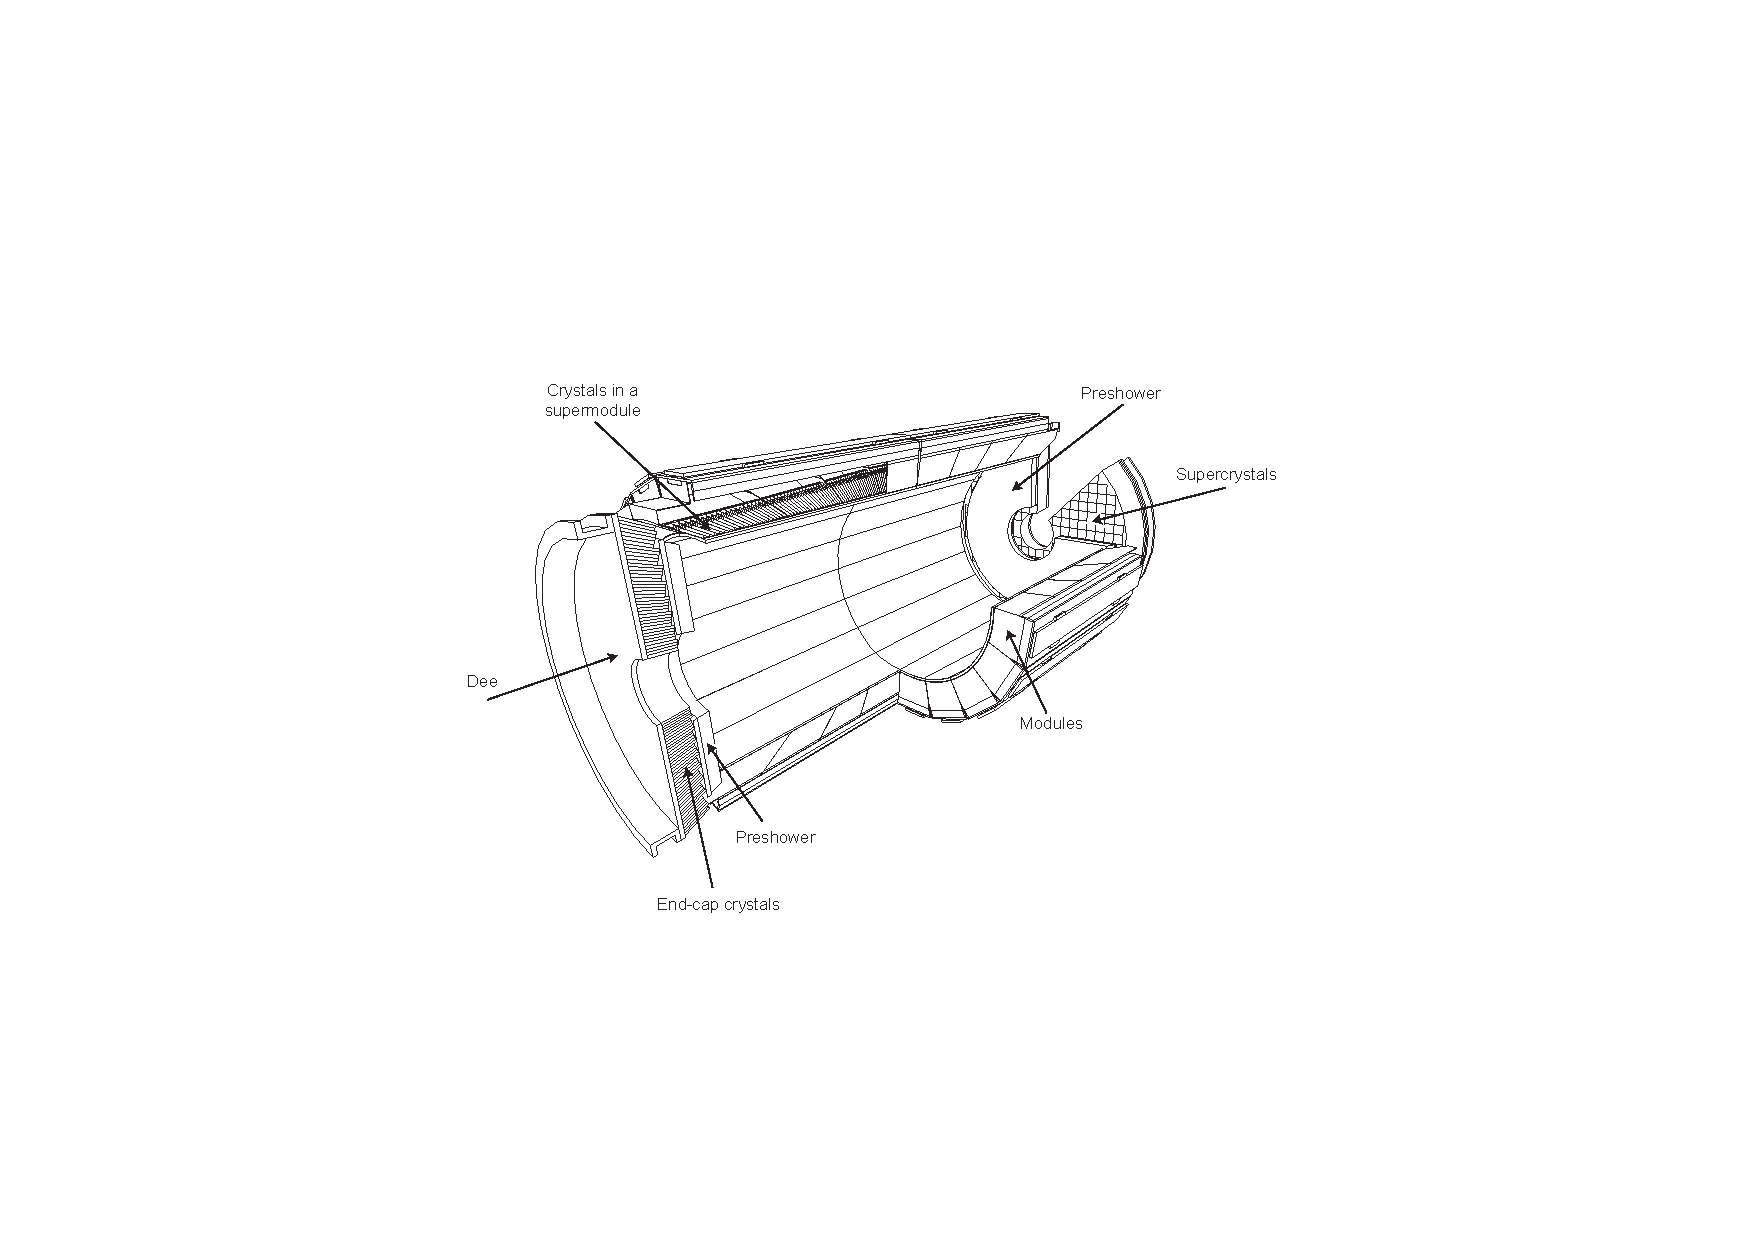
\includegraphics[width=0.48\textwidth]{figures/cms/CMS_ECAL}
  \caption{[left] The construction of the CMS electromagnetic calorimeter: lead-tungstate crystals
being tested in 2005. Figure taken from Ref.~\cite{CMS_ecal_crystal}.
[right] Schematic overview of the ECAL, showing the barrel modules that contain the crystals, the
endcaps, and the preshower detectors. Figure taken from Ref.~\cite{Chatrchyan:2008aa}.
  \label{fig:cms_ecal_crystal}}
\end{figure}

%%%%%%%%%%%%%%%%%%%%%%%%%%%%%%%%%%%%%%%%%%%%%%%%%%%%%%%%%%%%%%%%%%%%%%%%%%%%%%%%%%%%%%%%%%%%%%%%%%%%
\section{Hadron calorimeter \label{sec:cms_hcal}}

The hadron calorimeter is the last subdetector that is (mostly) located within the magnet coil. It
is designed to detect and absorb hadrons, such that the only particles leaving the HCAL are muons
and very weakly interacting particles such as neutrinos.
For this purpose it was built to be as hermetic as possible, staggering the detector layers to
make sure there are no gaps in straight lines that would allow hadrons to escape undetected.
Without this hermeticity it would be impossible to use the missing transverse energy as a way to
infer the presence of very weakly interacting particles. Many new physics searches, e.g. SUSY
searches, would lose most of their sensitivity. 

The HCAL consists of four subparts: the barrel (HB), outer barrel (HO), endcap (HE) and forward
(HF) sections. The barrel and endcap subsystems are sampling calorimeters, made of alternating
layers of dense absorber material (brass or steel) and fluorescent plastic scintillator tiles.
When a hadronic particle hits an absorber plate, an interaction can occur producing numerous
secondary particles. These secondary particles then flow through the successive layers of absorber
material, where they too can interact, resulting in a cascade or “shower” of particles.
As this shower develops, the particles pass through the layers of scintillators, causing them to
emit blue-violet light. This light is absorbed by wavelength-shifting optical fibres, which shift
the light into the green region of the spectrum, before being transported to the readout boxes by
clear optic cables. The amount of light that is collected is a measure of the energy of the passing
particle. Hybrid Photodiodes convert the optical signals into fast electronic signals which are
then sent to the data acquisition system. 

To fully absorb the particle showers, about one metre of absorber material is needed. As CMS is a
very compact detector, it was impossible to fit the full HCAL barrel inside the magnet coil. This
is the reason why the outer barrel, the tail-catcher, is located just behind the magnet coil, where
it ensures that the punch-through particles are absorbed as much as possible.  

The two hadronic forward calorimeters are positioned at either end of CMS, at 11.2\meter from
the interaction point, extending the coverage down to very high $|\eta|$. 
The HF receives the bulk of the particle energy contained in the collision, and so must be very
resistant to radiation. The design of the HF was primarily guided by the necessity to survive the
hostile conditions. Over 1000\unit{km} of quartz fibres are inserted into steel absorber
blocks. When particles traverse these fibres, they generate Cherenkov light. This light is then
transported through the fibers to photo multiplier tubes where it is converted into an electrical
signal. 
The HF is divided into two longitudinal segments, making it possible to distinguish the more shallow
showers generated by electrons and photons, from those generated by hadrons.

\begin{figure}[htpb]
  \centering
  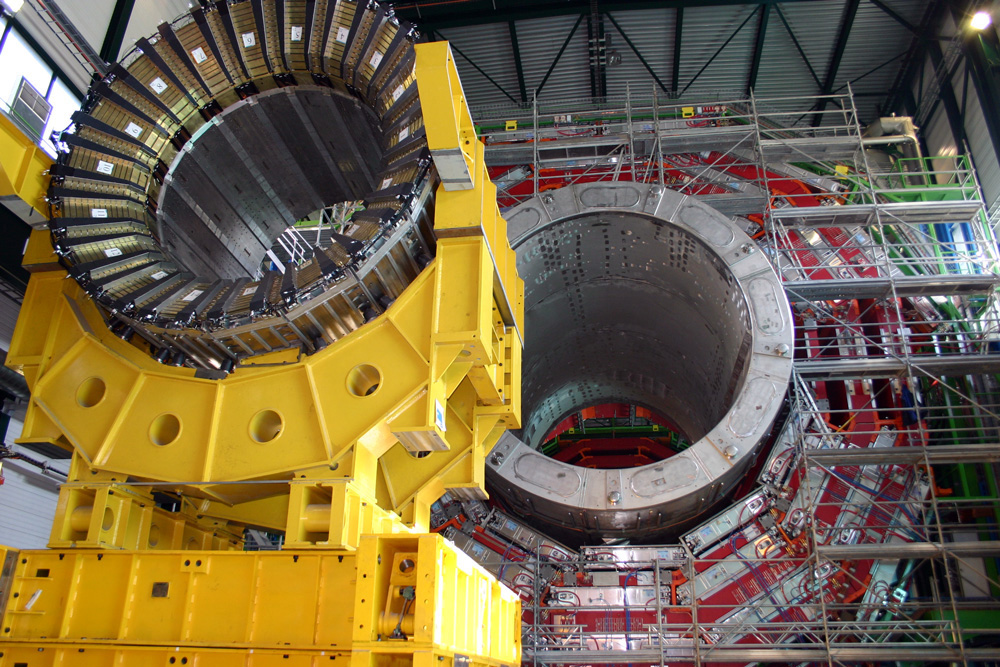
\includegraphics[height=0.2\textheight]{figures/cms/cms_hcal}
~
  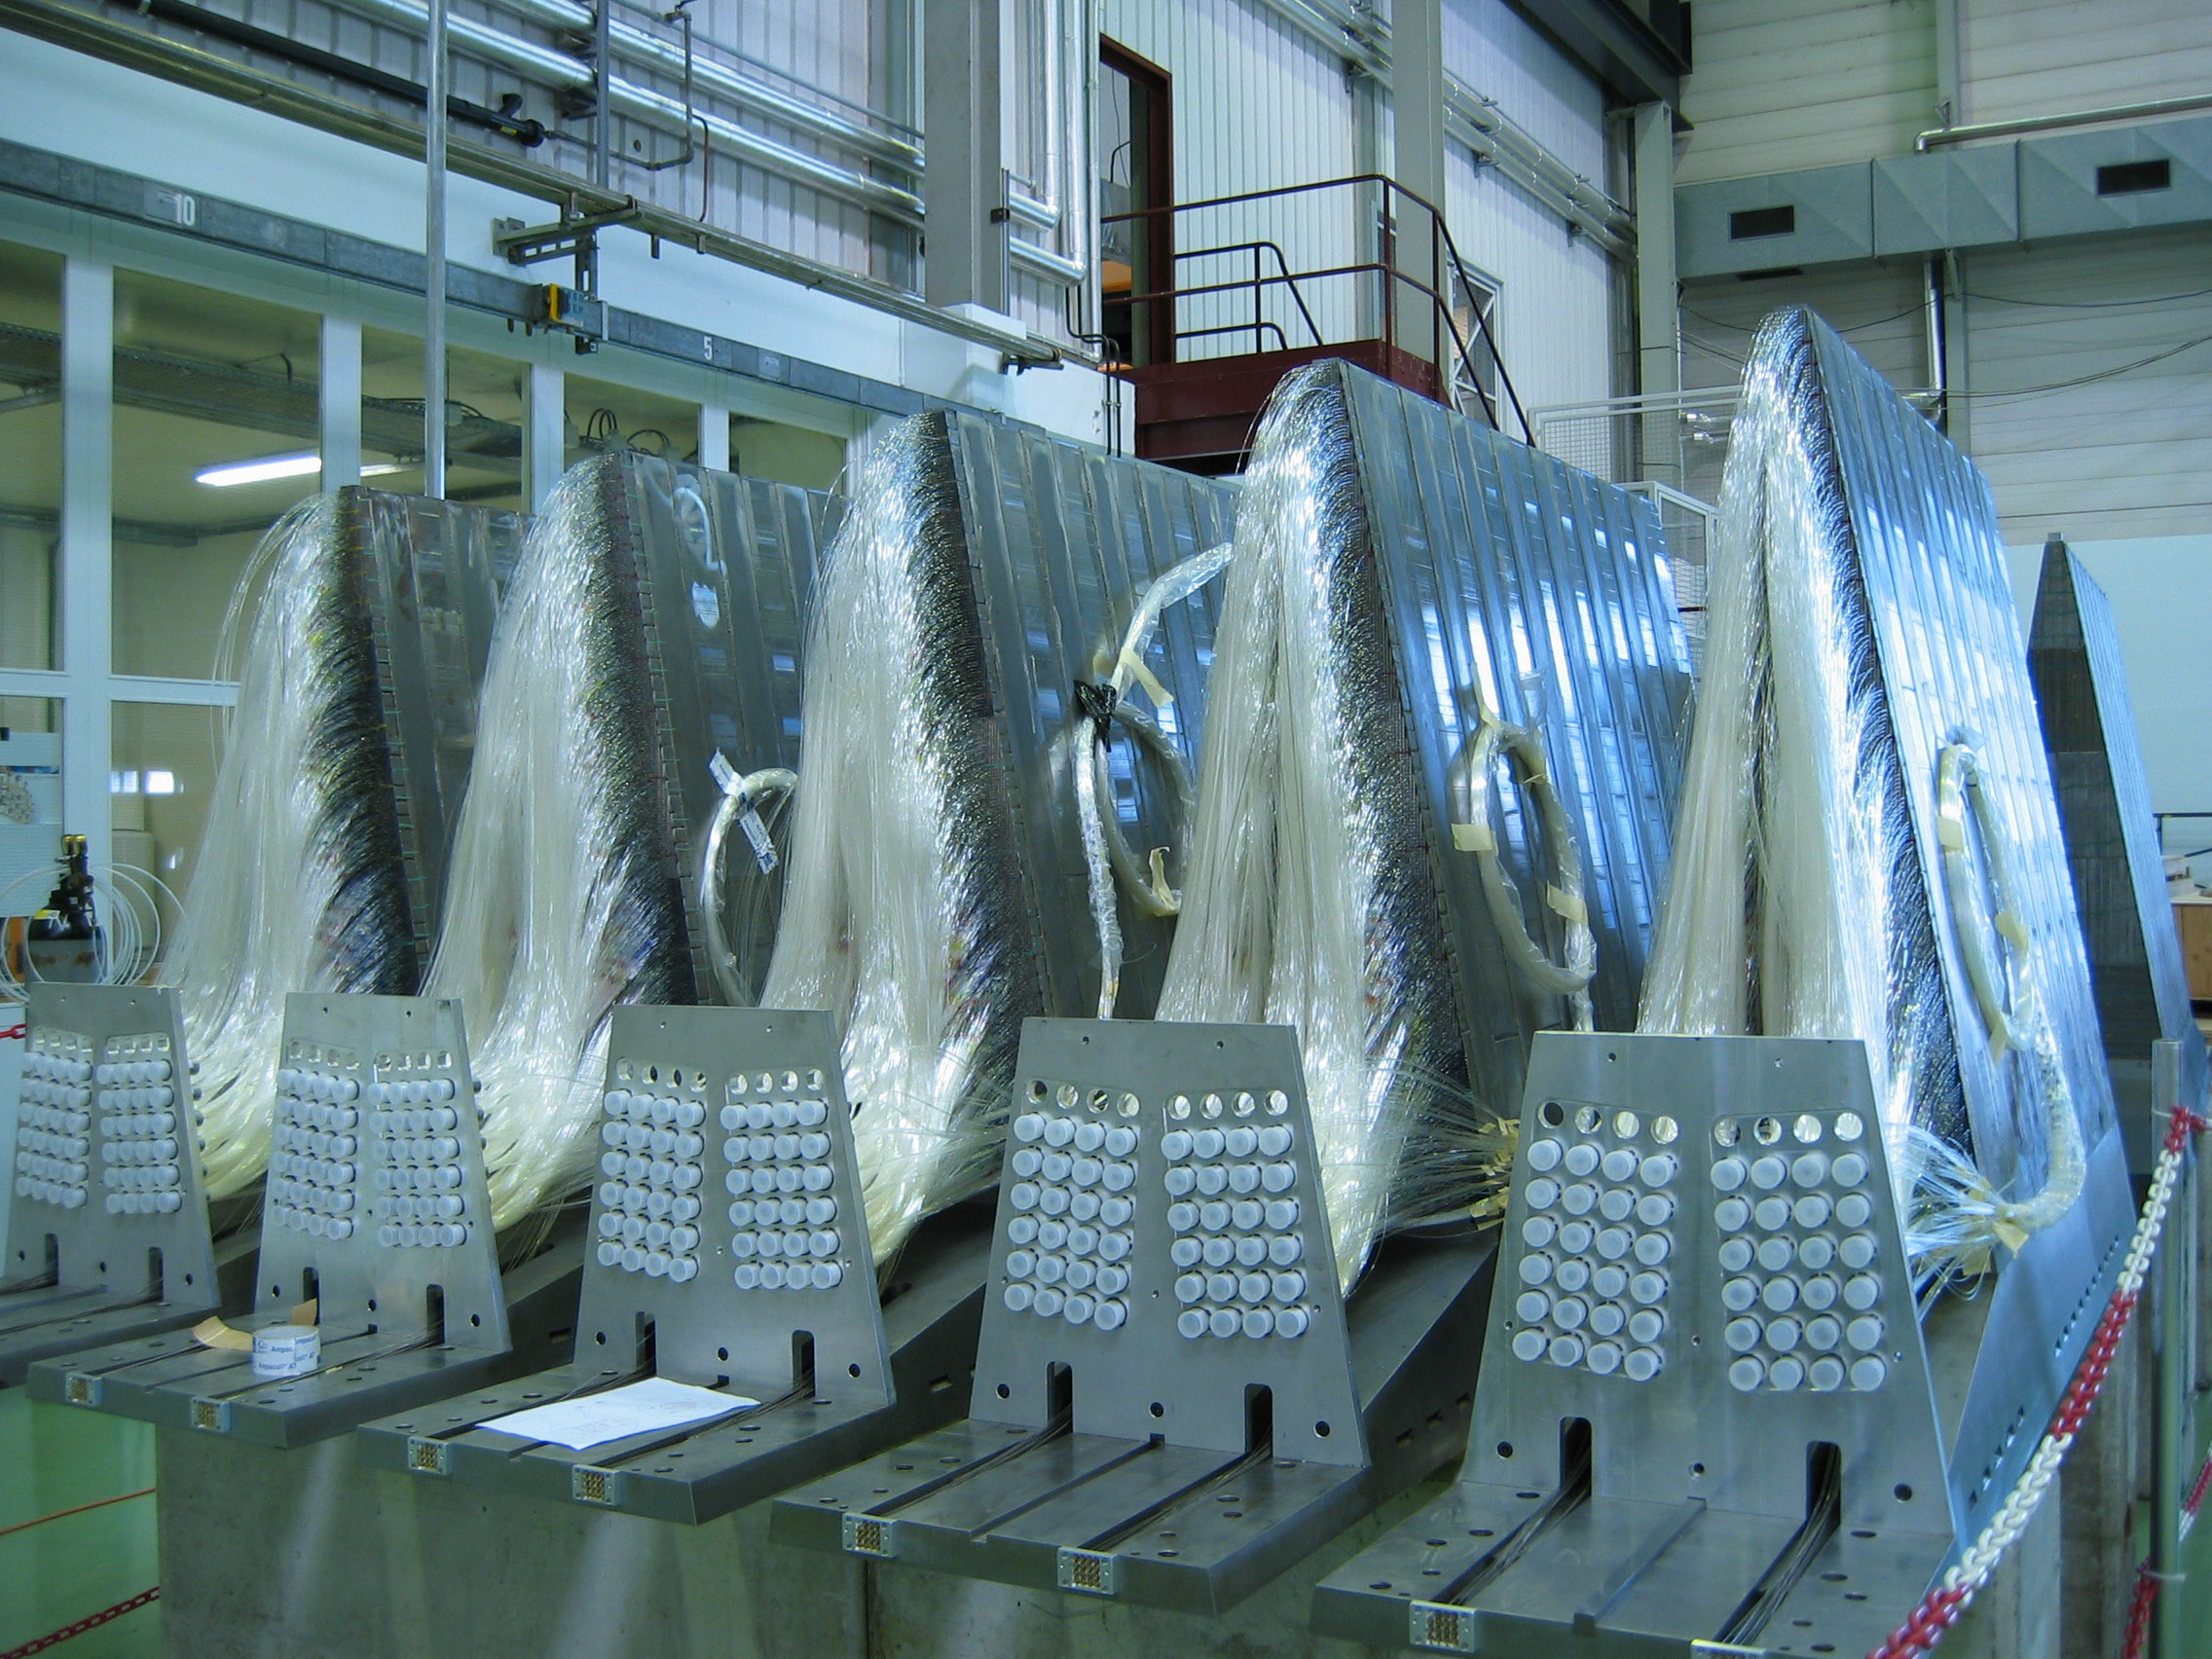
\includegraphics[height=0.2\textheight]{figures/cms/cms_hf_cds1431489}
  \caption{[left] Insertion of part of the barrel HCAL into the solenoid for the Magnet Test
and Cosmic Challenge in 2006. Figure taken from Ref.~\cite{CMS_hcal}.
[right] Segments of the forward HCAL during assembly, showing the quartz fibers inside the steel
wedges. Figure taken from Ref.~\cite{CMS_hf}. 
  \label{fig:cms_hcal}}
\end{figure}

%%%%%%%%%%%%%%%%%%%%%%%%%%%%%%%%%%%%%%%%%%%%%%%%%%%%%%%%%%%%%%%%%%%%%%%%%%%%%%%%%%%%%%%%%%%%%%%%%%%%
\section{Muon system \label{sec:cms_muon_system}}

Detecting muons, the heavier sibling of electrons, is one of the priorities of the Compact
\textit{Muon} Solenoid. Because it is 200 times heavier, a muon interacts less with material than
an electron, enabling it to penetrate several metres of iron, and pass through the calorimeter
systems unstopped. The muon chambers are, therefore, placed behind all the other subdetectors
where muons are the only particles that would register a signal. 
This also means that muons are not easily mistaken for any other particle, thus providing a very
clean signature. The Higgs boson decay to four muons is often referred to as the \textit{golden
channel} for exactly this reason, and it was indeed key to the Higgs boson discovery and the very
accurate measurement of its mass. 

The muon system consists of four muon stations, interleaved with the magnet return yoke, that track
the path of a muon. The momentum of the muon is then inferred from its curvature in the magnetic
field. Three different types of muon chambers are used: resistive plate chambers (RPCs) provide a
very fast trigger decision, while drift tubes (DTs) and cathode strip
chambers (CSCs) provide positional information and additional trigger information.
In the barrel region, DTs and RPC are arranged in concentric cylinders, whereas the endcap disks
contain different layers of CSCs and RPCs. Figure~\ref{fig:cms_muon_system} shows a schematic view
of the muon system, along with a picture from the barrel muon chambers in the return yoke. 

\begin{figure}[tpb]
  \centering
  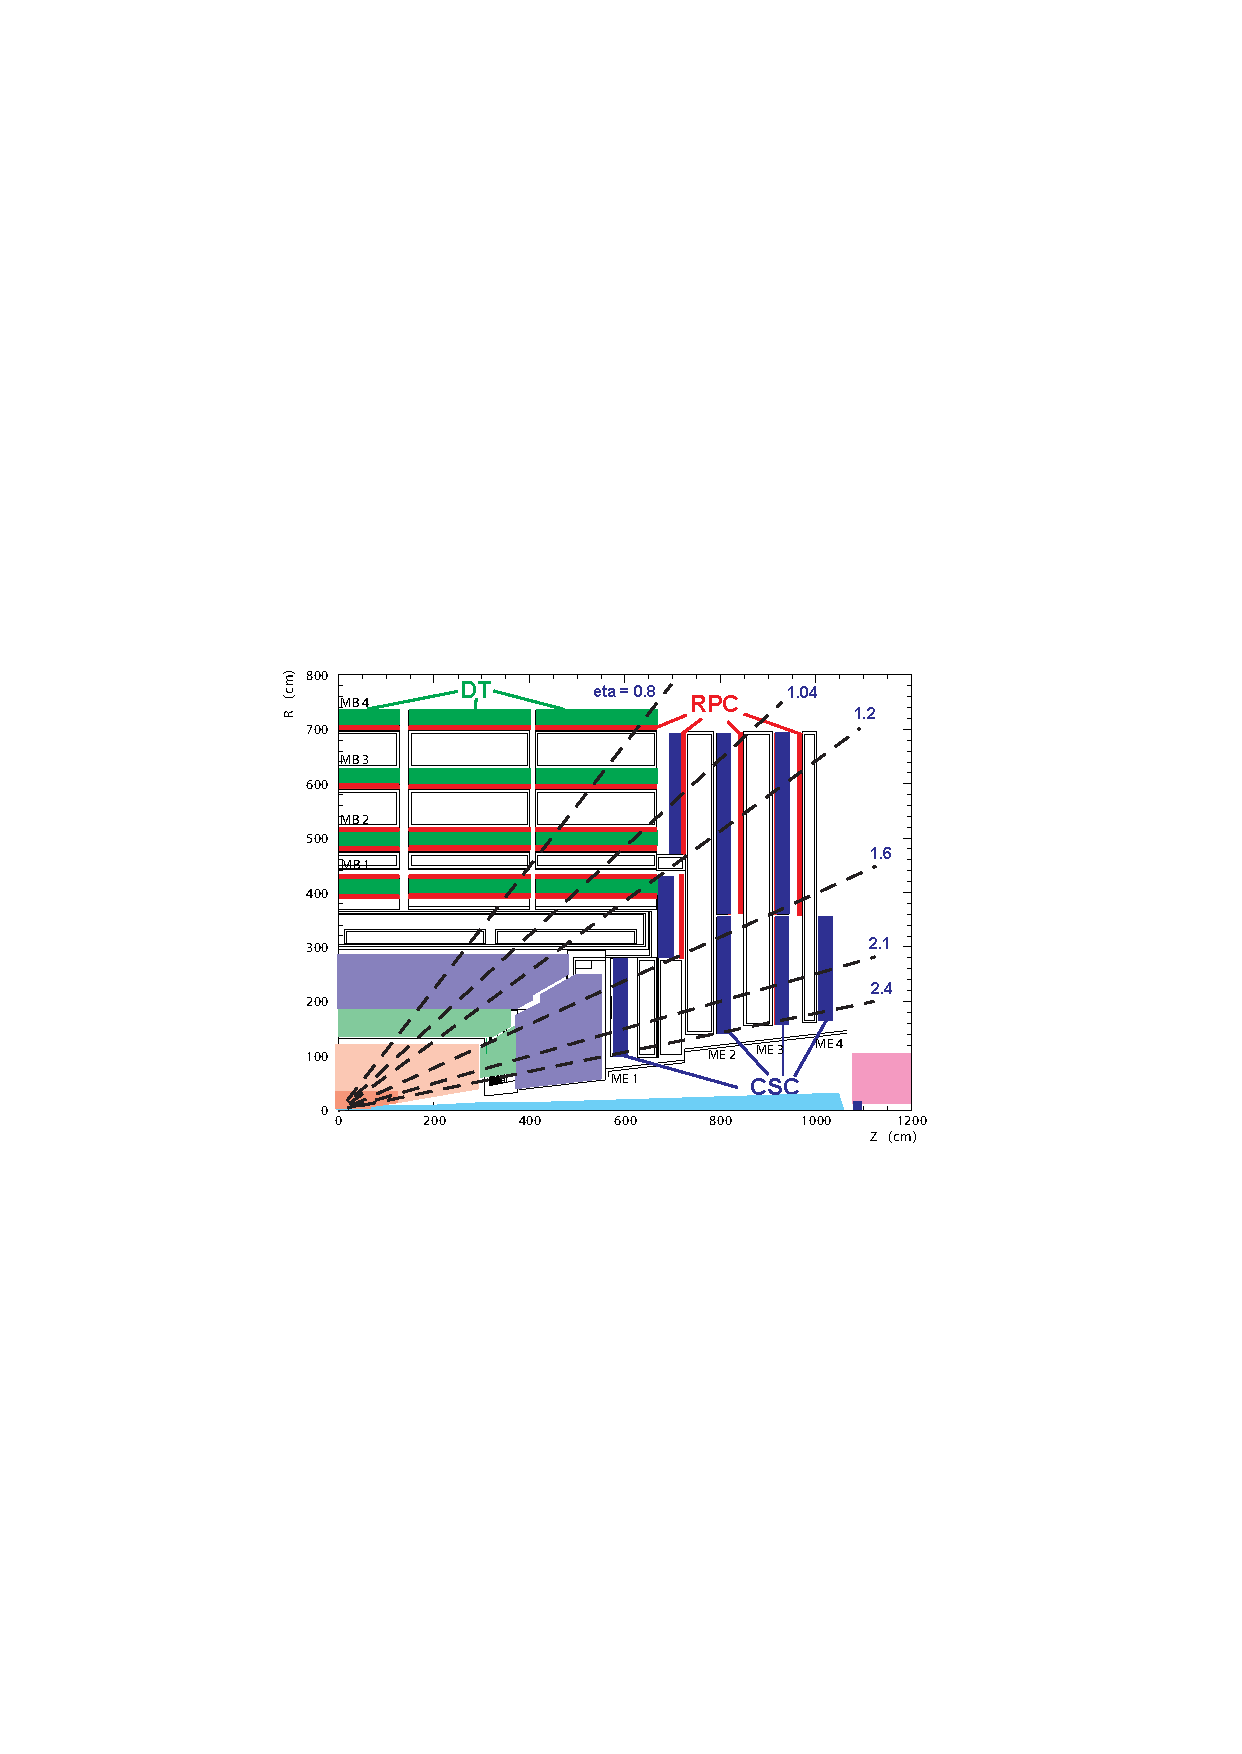
\includegraphics[height=0.205\textheight]{figures/cms/CMS_muon_system_diagram}
~
  \includegraphics[height=0.2\textheight]{figures/cms/cms_muon_system}
  \caption{[left] Schematic overview of one quarter of the CMS muon system, showing the DT, CSC and
RPC detectors. Figure taken from Ref.~\cite{Bayatian:922757}.
  [right] Muon chambers interspersed in the magnet return yoke. Figure taken from
Ref.~\cite{CMS_muon_system}.
  \label{fig:cms_muon_system}}
\end{figure}

\textbf{Drift tubes} contain a stretched wire within a gas volume. Any charged particles passing
through the gas create free electrons, which then drift towards the positively charged wire where
they are registered.  
Each CMS DT chamber, on average 2\meter by 2.5\meter in size, consists of 12 aluminium layers,
arranged in three groups of four, the superlayers, each containing up to sixty 4\cm wide drift
tubes.
The DTs can provide two coordinates for the position of the muon because the superlayers are placed
orthogonally to each other. The $(r, \phi)$ coordinate is measured by wires parallel to the
beampipe, while the $z$ coordinate is obtained from wires perpendicular to the beampipe. 
How far from the wire the muon actually passed, is determined from the electron drift speed and the
arrival time of the electrons at the wire.

\textbf{Cathode strip chambers} are more radiation resistant compared to drift tubes, and are,
therefore, used in the endcap disks where the magnetic field is uneven and particle rates are high. 
The CSCs are so-called multiwire proportional chambers, consisting of positively-charged anode wires
crossed with negatively-charged copper cathode strips inside a gas volume. Muons passing through
one of the 468 trapezoidally shaped CSCs ionize the gas, creating electrons that move
towards the anode wires, and positive ions that move towards the copper cathode. 
Because the strips and the wires are perpendicular, we obtain two position coordinates. The
wires provide the radial coordinate $r$, and the strips the $\phi$ coordinate. 
Given that the wires are very closely spaced, the CSCs are fast and can thus be used as input to the
trigger decision, besides performing the task of precision muon measurement. 

\textbf{Resistive plate chambers} are made of two parallel plates of a very high resistivity
material, a positively-charged anode and a negatively-charged cathode, which are separated by a gas
volume, the \textit{gap}. The CMS RPC system uses 610 double-gap modules comprising two gas gaps
with read-out strips in between. 
As for the other muon detectors, passing muons knock electrons out of gas atoms. These electrons
then initiate an avalanche which moves towards the anode. The avalanche is detected by the metallic
read-out strips. The pattern of the hit strips gives a measure of the muon momentum. Because RPCs
have a time resolution of just one nanosecond, they are very well suited be part of the muon trigger
system. 



%%%%%%%%%%%%%%%%%%%%%%%%%%%%%%%%%%%%%%%%%%%%%%%%%%%%%%%%%%%%%%%%%%%%%%%%%%%%%%%%%%%%%%%%%%%%%%%%%%%%
\section{Trigger and data acquisition \label{sec:cms_tdaq}}

At design specifications, CMS detects a proton bunch crossing every 25\unit{ns}. This means that
there are 40 million collisions per second, too much to fully read out, process and store for
further analysis. Reducing this amount of data to a more manageable few hundred events
per second is the role of the trigger system. It is of course of prime importance to keep the
interactions that could reveal new phenomena, such as supersymmetry, and discard those that provide
little new information. 
The decision to keep or throw out an event is made in two stages, at the Level-One (L1) Trigger and
the High-Level Trigger (HLT). Both of those systems will be discussed in the next sections. 

The enormous data production rate has another consequence. The collisions occur so fast that the
particles produced in one event have not yet left the detector when the next collision occurs. 
Associating each particle, and thus each detector signal, to the correct bunch crossing is only
possible because of the very good time resolution of the detectors, and the synchronization between
all the readout channels. 
Data from each subdetector is first collected in separate pipelines and is then sent off to the
switch networks to build the full event. Section~\ref{sec:cms_daq} will discuss in more detail how
the events are constructed.

\subsection{L1 Trigger \label{sec:cms_level_one}}

The L1 trigger is designed to make extremely fast decisions, based on relatively simple criteria,
reducing the data rate to about 100\unit{kHz}. 

When particles from a collision pass through the different subdetectors, they generate signals.
These signals are collected in buffers in the front-end electronics of the subdetectors themselves. 
A subset of the information is immediately passed along to the L1 trigger, which is housed
in a service cavern next to the detector. A total time of $3.2\mus$ is allocated for the transit to
the L1 trigger boards, choosing whether to keep or reject the event, and the transit back to the
front-end electronics to execute what was decided. During this time, the total amount of information
on a given collision needs to be kept in the buffers.
Less than 1\mus is allocated to the L1 trigger to perform the calculations needed to make the
decision. It is, therefore, built from custom hardware processors, fully optimized for the task at
hand. 

Because decisions have to made so quickly, it is impossible to use all available information, so
 only the calorimeters and the muon system are included. 
The trigger objects, such as photons, electrons, muons, and jets, are constructed by the global
calorimeter trigger and global muon trigger, using the reduced granularity and resolution data
sent to them from the front-end electronics. The objects are then passed to the Global Trigger,
which makes the decision to keep an event or not based on the number of objects above given \ET
or \pt thresholds, and/or on the total summed \ET or \ETm of the event. If the event is to be kept,
the high-resolution data is sent from the readout pipelines to the event builder and the High
Level trigger. 

\subsection{High Level Trigger \label{sec:cms_hlt}}

The High Level trigger~\cite{Adam:2005zf} is a computer farm that has access to the full event
information, and can therefore perform complex calculations similar to those made in the offline
analysis software. 
Each event reaching the HLT is sent to a separate processor which spends on average less than
0.1\second to make the final trigger decision, although for some events this can reach up to
1\second. 
The trigger software is set up in such a way that on average only a few hundred events per second
are kept and written to disk. 
A trigger path, a combination of object requirements that specifies which events should
be kept, can be as complex as needed, as long as the computation is fast enough. 
To facilitate this, the trigger paths are set up in such a way that events are discarded as soon as
possible, before reaching the more time consuming parts of the code. 
An example of this could be the use of jets constructed from only calorimeter information, before
adding the information from the numerous tracker readout channels to improve precision. 
Each event that is kept receives a set of tags associated with the separate trigger paths that were
fulfilled. These tags are later used to sort the data into so-called primary datasets. 


% HLT refs \cite{Adam:2005zf,Agostino:2009nva}

\subsection{Data acquisition \label{sec:cms_daq}}

The CMS data acquisition (DAQ) system~\cite{Cittolin:578006} comprises different components, which
are illustrated in Fig.~\ref{fig:cms_event_builder}. 
The about 700 detector front-end drivers store the data from the detector front-end electronics upon
the reception of an accept signal from the L1 Trigger. The data are then read by the readout system
and stored until they are sent to the HLT for further processing. 
The builder network provides the interconnections between the readout and the HLT systems, running
with a bandwidth of 100\unit{GB/s}. It takes care of building the full events out of the different
data fragments from the separate parts of the detector. The builder networks consists of 500 builder
units, each of which will assemble the data for one event. 
Once the event is assembled it is passed to one of the HLT processors associated to that particular
builder unit. As soon as the HLT decision is made, that decision is transferred back to the builder
unit which then either discards the event, freeing up the memory, or sends it to the storage
manager to be written to disk.
Apart from building the events, the DAQ also provides detector control and monitoring services.

\begin{figure}[htpb]
  \centering
  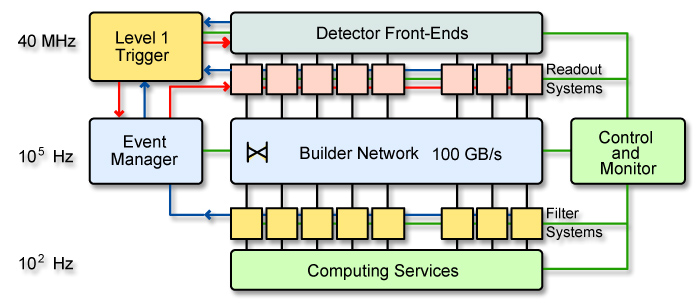
\includegraphics[width=0.8\textwidth]{figures/cms/cms_event_builder}
  \caption{ General architecture of the CMS DAQ System. Figure taken from
Ref.~\cite{Bayatian:922757}.
  \label{fig:cms_event_builder}}
\end{figure}


% refer to next chapter for event reconstruction

%%%%%%%%%%%%%%%%%%%%%%%%%%%%
%% Event generation 
%%%%%%%%%%%%%%%%%%%%%%%%%%%%


In this section I will explain in more detail the various techniques employed by the most common
event generators. In particular, I will focus on \MADGRAPH~\cite{Alwall:2011uj,Alwall:2014hca} and
\PYTHIA~\cite{Sjostrand:2006za}, the programs that generated the events for most of the processes
used in the Razor Boost analysis, presented in Chapter~\ref{chap:razorboost}. 
The following sections are based on
Refs.~\cite{Campbell:2006wx,Salam:2010zt,Skands:2011pf,Buckley:2011ms,Sjostrand:2006za,Alwall:2011uj
,Alwall:2014hca}. 

\subsection{Matrix element generators \label{sec:event_matrix_element_generators}}

As explained previously, the hard interaction can be described using matrix elements, which can be
computed, at least in principle, order by order using perturbation theory. 
There are a variety of programs available that calculate the tree-level diagrams numerically,
and integrate over the relevant phase space. The most widely used are \MADGRAPH, now merged
into \textsc{MG\_aMC@NLO}, and \textsc{Alpgen}~\cite{Mangano:2002ea}. 
There are no inherent limits to the number of final state particles that could be produced with
these programs, although, in practice, the computation is limited by the factorial growth of the
number of diagrams as we go higher in multiplicity of final state particles. 
In this section I will explain the basic algorithms used by \MADGRAPH to generate events at leading
order accuracy. For all details, and a discussion on how event generation at next-to-leading order
precision is done, I refer to Refs.~\cite{Alwall:2011uj,Alwall:2014hca}.

\MADGRAPH allows for automatic generation of matrix elements for collider physics processes, such as
decays and $2 \rightarrow n$ scatterings. 
As the user, one first specifies the desired process in terms of initial and
final state particles. It is possible to exclude or require the presence of s-channel resonances,
and one can force a particular decay chain. 
Once the process is fully specified, \MADGRAPH computes all Feynman diagrams that can contribute,
and writes process-specific code to compute the matrix elements. The user is not restricted
to models implemented by default in \MADGRAPH. Feynman rules for any (new) physics model can be
obtained via \textsc{FeynRules}~\cite{Alloul:2013bka} and passed to \MADGRAPH via the standardized
UFO format~\cite{Degrande:2011ua}. 

The algorithm to determine all relevant diagrams recursively creates sub-diagrams by merging legs.
It can be most easily explained by considering a simple example. We will go through the different
steps for the diagram generation of $e^+ e^- \rightarrow \cPqu \cPaqu \cPg$. The relevant vertices
in the standard model are $(e^+ e^- \gamma)$, $(e^+ e^- \cPZ)$, $(\cPqu \cPaqu \gamma)$, $(\cPqu
\cPaqu \cPZ)$, and $(\cPqu \cPaqu \cPg)$. Before the start of the algorithm, the initial state
particles are flipped such that only outgoing particles are present. We then proceed as follows.
\begin{enumerate}
  \item  First it is checked whether there is a vertex including all particles. In this example
this is not the case. 
  \item Then all possible two-particle groupings are performed, and the groups are replaced by a
single particle according to the allowed vertices. An example is the grouping $(e^+ e^-) \cPqu
\cPaqu \cPg$, which results in the replacements $(\gamma) \cPqu \cPaqu \cPg$ and $(\cPZ) \cPqu
\cPaqu \cPg$. The full list of groupings and replacements for this example is shown in
Table~\ref{tab:madgraph_diagrams}. Each option gets assigned a number according to how many groups
were replaced, here either 1 or 2. 
  \item All combinations after the replacement for which fewer than two groupings were replaced,
i.e. the first seven in the table, are discarded because they cannot give rise to valid diagrams, or
would lead to double counting if grouped further. 
  \item For the remaining combinations the presence of a valid vertex is checked. Only the final
four options have a valid vertex in this example. These diagrams are thus added to the list of
possible diagrams. 
  \item The iteration ends here because any further grouping of these valid diagrams would result
in a state that contained less than two replacements. The four diagrams that were generated are
shown in Fig.~\ref{fig:madgraph_diagrams}.
\end{enumerate}

\begin{table}[t]
  \caption{Steps for the diagram generation algorithm employed in \MADGRAPH. Table taken from
Ref.~\cite{Alwall:2011uj}. 
  \label{tab:madgraph_diagrams}}
  \begin{center}
  {\setlength{\tabcolsep}{1.5eM}
  \begin{tabular}{l l l}
  \toprule
  First iteration & Groupings & Replacements \\
  \midrule
  \multirow{17}{*}{$e^-,e^+,\cPqu,\cPaqu,\cPg$} & \multirow{2}{*}{$(e^-,e^+),\cPqu,\cPaqu,\cPg$} &
$(\gamma), \cPqu, \cPaqu, \cPg$ \\
  & & $(\cPZ), \cPqu, \cPaqu, \cPg$ \\ \cmidrule(lr){2-3}
  & \multirow{3}{*}{$e^- , e^+ , (\cPqu, \cPaqu), \cPg$} & $e^- , e^+ , (\gamma), \cPg$ \\
  & & $e^- , e^+ , (\cPZ), \cPg$ \\
  & & $e^- , e^+ , (\cPg), \cPg$\\ \cmidrule(lr){2-3}
  & $e^- , e^+ , (\cPqu, \cPg), \cPaqu$ & $e^- , e^+ , (\cPqu), \cPaqu$\\ \cmidrule(lr){2-3}
  & $e^- , e^+ , \cPqu, (\cPaqu,\cPg)$ & $e^- , e^+ , \cPqu, (\cPaqu)$\\ \cmidrule(lr){2-3}
  & \multirow{6}{*}{$(e^- , e^+ ), (\cPqu, \cPaqu), \cPg$} & $(\gamma), (\gamma), \cPg$ \\
  & & $(\gamma), (\cPZ), \cPg$\\
  & & $(\gamma ), (\cPg), \cPg$\\
  & & $(\cPZ ), (\gamma), \cPg$\\
  & & $(\cPZ ), (\cPZ), \cPg$\\
  & & $(\cPZ ), (\cPg), \cPg$\\ \cmidrule(lr){2-3}
  & \multirow{2}{*}{$(e^- , e^+ ), (\cPqu, \cPg), \cPaqu$} & $(\gamma ), (\cPqu), \cPaqu$\\
  & & $(\cPZ ), (\cPqu), \cPaqu$ \\ \cmidrule(lr){2-3}
  & \multirow{2}{*}{$(e^- , e^+ ), \cPqu, (\cPg, \cPaqu)$} & $(\gamma ), \cPqu, (\cPaqu)$\\
  & & $(\cPZ ), \cPqu, (\cPaqu)$\\ 
  \bottomrule
  \end{tabular}
  }
  \end{center}
\end{table}

\begin{figure}
  \centering
  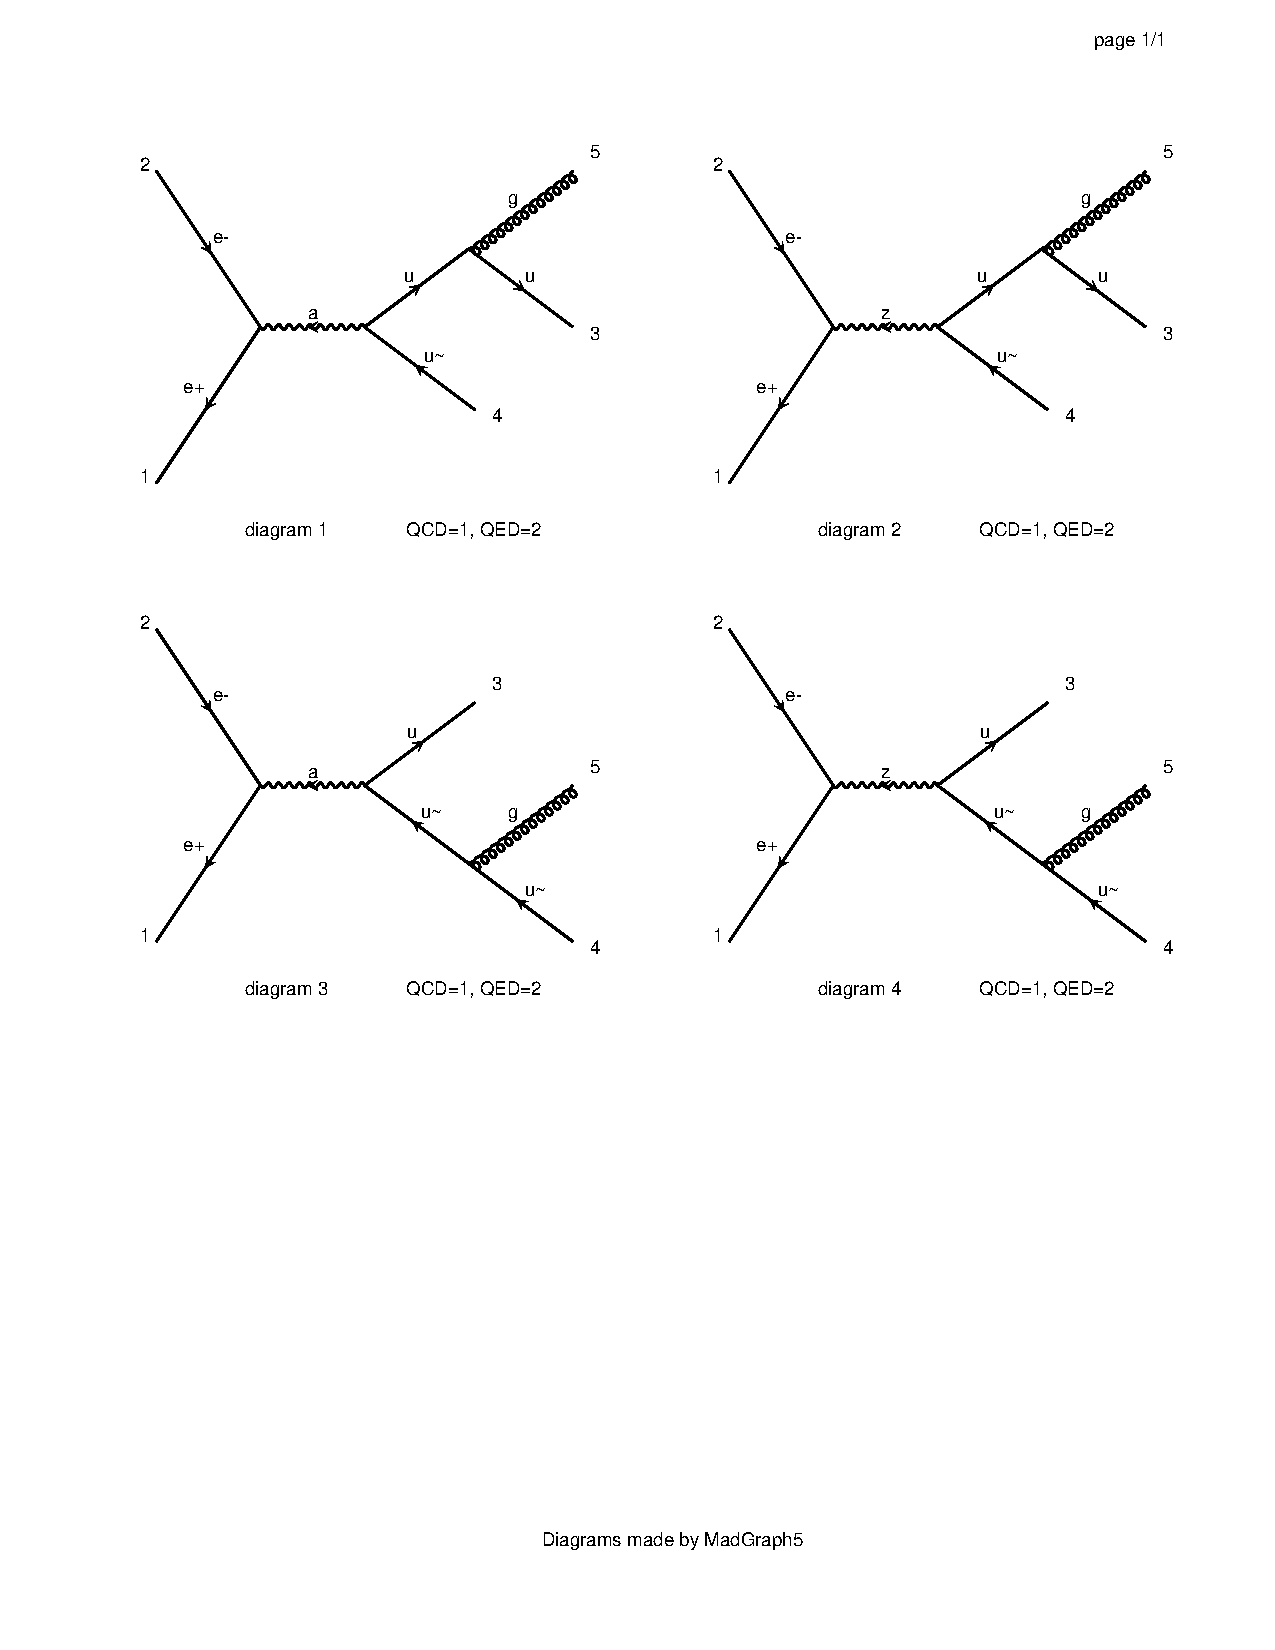
\includegraphics[width=0.9\textwidth, clip=true, trim=1cm 10.5cm 1cm 2cm]
{figures/eventreco_generation/matrix1}
  \caption{Feynman diagrams for the process $e^+ e^- \rightarrow \cPqu \cPaqu \cPg$
  \label{fig:madgraph_diagrams}}
\end{figure}

The computation of the squared matrix element for a given process is done via calls to helicity
wavefunctions and amplitudes. Helicity amplitudes work on the amplitude level, in contrast to the
methods using contraction of Lorentz-indices that work on squared amplitudes.  A big advantage is
that the complexity of the calculation grows linearly rather than quadratically, and that diagrams
are factorized such that the subcomponents, i.e. the helicity wavefunction calls, can be reused
between diagrams. 
A helicity wavefunction is first generated for each external leg in any diagram using the
\textsc{ALOHA}~\cite{deAquino:2011ub} package. 
These wavefunctions are then combined into new wavefunctions corresponding to the propagators in the
diagram by successive helicity wavefunction calls. The final vertex then corresponds to a helicity
amplitude call which returns the value of the amplitude corresponding to this particular diagram.

Particle decays are treated in the same way as the production, allowing for efficient treatment of
multiprocesses with the same decay pattern. An example of this is the process $\Pp \Pp \rightarrow
\W^+$, with $\W^+ \rightarrow \ell^+ \nu_l$. This process contains the production
processes, $\cPqu \cPaqd \rightarrow \W^+$, $\cPaqd \cPqu \rightarrow \W^+$, $\cPqc \cPaqs
\rightarrow \W^+$, $\cPaqs \cPqc \rightarrow \W^+$, and the decay processes $\W^+ \rightarrow
e^+ \nu_e$, $\W^+ \rightarrow \mu^+ \nu_\mu$, $\W^+ \rightarrow \tau^+ \nu_\tau$. 
All these building blocks only need to be generated once, and can then be combined in all possible
ways to obtain the full matrix element.  
 
Once the code for the process under consideration is generated, we can start generating events.
\MADGRAPH uses a so-called run\_card as configuration for the event generation. In this card the
user can specify how many events to produce, which phase space cuts to apply, which parton
distribution functions to use, how to choose the renormalization scale, etcetera. Using this
configuration, the numerical integration of the matrix element squared over the appropriate phase
space is performed, and unweighted events are finally obtained. 

The phase space to integrate is usually high-dimensional, and contains many peaks, which are often
 related to propagators in one of the diagrams becoming large. 
Efficient sampling techniques are thus critical for the performance of the event generation.
Standard MC integration techniques such as importance sampling have the drawback that you need to
know a lot about the function $f$ you wish to integrate in order to find an appropriate, more
well-behaved, function $g$ to help the MC integration. 
Since this is not usually the case for these phase space integrals, the \MADGRAPH program implements
a custom integration method, called single-diagram-enhanced multi-channel
integration~\cite{Maltoni:2002qb}.
The method works as follows.
Assume that the function to be integrated could be written in terms of a basis of $n$ functions
$f_i$,
\begin{equation}
  f = \sum_{i=1}^n f_i, \text{ with } f_i > 0, \quad \forall i,
\end{equation}
such that the peak structure of each $f_i$ can be efficiently mapped by a single function $g_i$.
Then, the integration of $f$ reduces to a sum of $n$ independent, and simpler, integrations.
\begin{equation}
  I = \int d\Phi f(\Phi) = \sum_{i=1}^n \int d\Phi g_i(\Phi) \frac{f_i(\Phi)}{g_i(\Phi)} =
\sum_{i=1}^n I_i .
\end{equation}
For a generic integration problem, such a basis might be too difficult to identify, but here we can
use the physical content of the process and decompose $f$ according to the single Feynman diagrams, 
\begin{equation}
  f_i = \frac{|A_i|^2}{\sum_i |A_i|^2} |A_{\text{total}}|^2
\end{equation}
where $A_i$ is the amplitude corresponding to a single Feynman diagram and $A_{\text{total}}$ is the
total amplitude. Finding the suitable mapping $g_i$ is straightforward, since it can be
derived from the known propagator structure of the corresponding Feynman diagram. 
Since the $I_i$ can be computed independently and then combined, this method is inherently parallel
in nature, allowing the use of computer clusters to speed up the computation and thus facilitating
the generation of more complicated processes.  

Because of its good performance, ease of use, and flexibility, \MADGRAPH is the standard
matrix-element generator used by the CMS experiment. 
Other generators are still used for dedicated processes, or to derive systematic
uncertainties on the prediction coming from the details and approximations made by the various 
event generators. 

The result of the event generation is a set of final state, hard particles. Very
soft or collinear particles cannot be computed by matrix-element generators, as the matrix element
diverges. The next section will cover parton shower programs, whose purpose is exactly to deal with
soft and collinear radiation. Section~\ref{sec:event_matching} will discuss a technique on how to
match the matrix element computation with the parton shower to obtain the best of both worlds. 



\subsection{Parton shower}

The fixed-order matrix-element MC programs discussed in the previous section provide a powerful
combination of accuracy and flexibility as long as you want to calculate infrared and collinear safe
observables -- such as jets, $\W$ or $\cPZ$ bosons, but not pions, kaons, etcetera -- and
don’t need to study regions of phase space that involve disparate physical scales. An example of
the latter could be requiring a heavy boson to have a \pt much smaller than its mass, leading to
large coefficients at all orders in the perturbative expansion.
These defects are related to the presence of soft and collinear divergences in the calculations.
Real life does not diverge, however. We thus need a different approach to tackle the soft and
collinear part of the phase space. This approach is the parton shower. 

Parton shower algorithms, such as the one implemented in \PYTHIA, describe the evolution in
momentum transfer from the high scales associated with the hard process down to the low scales, of
order 1\GeV, associated with the confinement of the partons it describes into hadrons. 
In analogy with bremsstrahlung of photons in QED, a parton (quark or gluon) with high momentum will
have some probability to radiate a gluon. This gluon can then radiate more gluons, or it can split
in a $q\bar{q}$ pair. This process repeats itself until the energy of the quarks and gluons becomes
too low, and hadronization begins. Hadronization is a non-perturbative process, but fortunately it
is universal, i.e. it does not depend on the hard interaction, but only on the partons at the low
scale after the parton shower.

The probabilities for the various parton splittings are encompassed in the splitting functions,
$P_{j\leftarrow i}$, which were already mentioned briefly in Section~\ref{sec:event_pdfs}.
Let us first introduce the variable $t$ as
\begin{equation}
  t = \ln\frac{Q^2}{\Lambda^2},
\end{equation}
with $\Lambda$ the QCD scale. We then find for the differential
\begin{equation}
  \text{d}t = \text{d}\ln Q^2 = \frac{\text{d}Q^2}{Q^2}.
\end{equation}
We can view $t$ as a kind of time in the evolution of the parton shower. The smaller $t$, and
thus the lower the scale, the further along in the shower process we are. 
In terms of the variable $t$, we can write the differential probability for a parton $i$ to branch
into any parton $j$ with momentum fraction $z$ in the following way,
\begin{equation}
  \text{d}\mathcal{P}_i = \sum_j \frac{\alpha_S}{2\pi} P_{j\leftarrow i}(z)\text{d}t\text{d}z,
\label{eq:splitting}
\end{equation}
with the different splitting functions in the collinear limit given by
\begin{align}
  P_{q\leftarrow q}(z) &= C_F \frac{1 + z^2}{1 - z}, & 
  P_{g\leftarrow q}(z) &= C_F \frac{1 + (1-z)^2}{z}, \\
  P_{g\leftarrow g}(z) &= C_A \frac{z^4 + 1 + (1-z)^4}{z(1-z)}, &
  P_{q\leftarrow g}(z) &= T_R (z^2 + (1-z)^2), 
\end{align}
where $C_F$ and $C_A$ are colour factors and $T_R$ is a constant depending on the definition of
$\alpha_S$. 
There are two sets of divergencies that occur in the computation of the branching probability: when
the radiated parton becomes extremely soft, or when it becomes collinear with the original parton. 
The cases where this occurs can in fact not be resolved in any physical measurement. Two exactly
collinear partons look exactly like one parton with the same total momentum. We should thus impose
a resolution criterion. Often the chosen criterion is that the relative transverse momentum
between the two partons is larger than some cutoff scale $Q_0$. Imposing this cutoff, then results
in a finite resolvable emission probability. Because the total probability of something happening
has to be unity, we can find the probability to not have a resolvable emission as one minus the
resolvable emission probability. In this way we have avoided computing the divergent pieces, which
would have to be added to the divergent loop-correction to the hard process in order to cancel.

Since Eq.~\ref{eq:splitting} is a completely general expression that does not depend on the hard
process, we can iterate it, using it on a parton resulting from the hard process to generate
one branching and then treating the new final state as the hard process, generating another
splitting from it, and so on. In what follows we will discuss how this shall be done in practice.

The integral of the branching probability over all allowed $z$ values, according to the
particular resolution criterion imposed, and for a given $t$ value, is defined as
\begin{equation}
  \mathcal{I}_{j\leftarrow i}(t) = \int dz \frac{\alpha_S}{2\pi} P_{j\leftarrow i}(z)
\end{equation}
The naive probability that a resolved branching occurs during a small range of $t$ values, $\delta
t$, is given by 
\begin{equation}
 \sum_j \mathcal{I}_{j\leftarrow i}(t) \delta t,
\end{equation}
where we did not take into account anything which could have happened during the parton shower,
before that time. The probability for no resolved emission to occur is then simply given by $1 -
\sum_j \mathcal{I}_{j\leftarrow i}(t) \delta t$. 
If the evolution of parton $i$ starts at $t_{\text{max}}$, then the probability that the parton
has not yet branched later in the shower, when $t < t_{\text{max}}$, is given by
the product of the probabilities that it did not branch in any of the small intervals $\delta t$
between $t$ and $t_{\text{max}}$. In other words, letting $\delta t \rightarrow 0$, the no-branching
probability at time $t$, given starting point $t_{\text{max}}$, exponentiates, and is given by
\begin{equation}
  \mathcal{P}_{\text{no-branching}}(t_{\text{max}},t) = \exp 
  \left\{ - \int_t^{t_{\text{max}}} dt' \sum_j \mathcal{I}_{j\leftarrow i}(t') \right\} .
\end{equation}
The actual differential probability that the first resolved branching of parton $i$ occurs at `time'
$t$, which is the actual question we wish to answer, is thus given by
\begin{align}
  \frac{\text{d}\mathcal{P}_i}{\text{d}t} &= -
\frac{\mathcal{P}_{\text{no-branching}}(t_{\text{max}},t)}{\text{d}t} \\
 &= \left( \sum_j \mathcal{I}_{j\leftarrow i}(t)\right) \exp \left\{ - \int_t^{t_{\text{max}}} dt'
\sum_j \mathcal{I}_{j\leftarrow i}(t) \right\}, \label{eq:prob_first_branch}
\end{align}
where the first factor in Eq.~\ref{eq:prob_first_branch} is the naive probability mentioned above,
and the second term is an exponential suppression, similar to that found in the formula for
radioactive decay, to account for the fact that if a parton has already branched at $t'$, it can no
longer branch at $t$. 
This exponential factor, the probability to not branch above a certain scale, here
contained in the variable $t$, is called the Sudakov form factor, $\Delta_i(t_max,t)$. 

Implementing this in a Monte Carlo program is conceptually straightforward. 
First, a random number $r$ is sampled uniformly between 0 and 1. Then the value for $t$ such that 
$\Delta_i(t_max,t) = r$ is determined. If the solution is above the cutoff $t_0$, corresponding to
the resolution $Q_0$, then a resolvable branching is generated with scale $t$, otherwise the shower
evolution is terminated. In case a resolvable branching is to be generated, a $z$ value is chosen
according to the splitting functions $P_{j\leftarrow i}(z)$, and then the algorithm is started
again. 
Of course, in practice one has to take into account several complications. 
Different approaches exist for deciding what the initial scale $t_{\text{max}}$ should be.
This scale has to match the hard interaction, and could thus be the largest virtuality in the hard
scatter, but could also be the centre-of-mass energy. 
The Sudakov form factor is also not necessarily easily invertible analytically, which can dealt
with by using the so-called veto-algorithm. 
Apart from final state
showers, such as explained here, the initial state also undergoes showering. There it is important
to properly match the parton shower with the PDF treatment, as well as ensure on-shell partons that
take part in the hard interaction.
For all details on how this is fully implemented in the \PYTHIA shower routine, I refer to
the manual~\cite{Sjostrand:2006za}. 

At the end of the parton shower procedure, we end up with many more partons than we had directly
after the hard interaction, all which should be described at the low scale, via non-perturbative
models. The most widely used hadronization model will be discussed in
Section~\ref{sec:event_hadronization}. 


\subsection{Matching the matrix element to the parton shower \label{sec:event_matching}}

On the one hand, parton shower MC programs provide an excellent event description in regions which
are dominated by soft and collinear gluon emission, including the hadron-level details that are
necessary for the proper simulation of detector effects. 
On the other hand, matrix element calculations provide a good description of processes where
the partons are energetic and widely separated. They also include the effects of
interference between amplitudes with the same external partons. 
The best possible event description can thus only be achieved by combining both approaches.
However, the direct addition of the two techniques can lead to double-counting in kinematic regions
where the two calculations overlap. This is of particular importance when merging samples for
different parton multiplicities, as illustrated in Fig.~\ref{fig:overlap}.
We will thus need a matching between the matrix element
and the parton shower to ensure the proper removal of these overlaps.
There are several techniques available to perform this matching. I will focus here on the so-called
\textit{MLM matching}~\cite{Alwall:2007fs}, which is the technique used in CMS to match \MADGRAPH
with \PYTHIA. The MLM technique comprises three main steps, the first of which is done at the
matrix element level. Then the partons are showered, and finally the shower jets are matched to the
hard partons. 
In next paragraphs I will discuss each step in more detail. 


\begin{figure}[t]
  \centering
  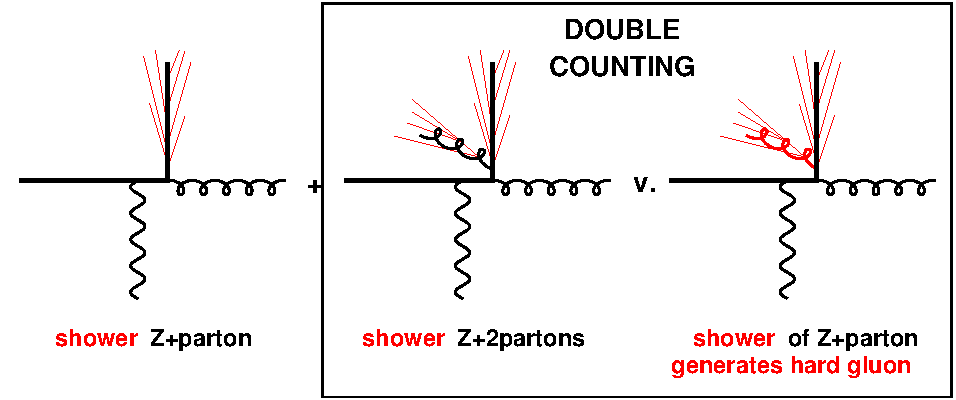
\includegraphics[width=0.8\textwidth]{figures/eventreco_generation/overlap}
  \caption{ Illustration of the double-counting issues that can arise if one naively attempts to
shower $\cPZ+$parton and $\cPZ+2$parton events. Partons generated by the matrix element are
shown in black, whereas the effects of the parton shower are shown in red. Showering the 1-parton
sample could lead to the generation of a hard gluon, which is already included in the matrix-element
description of the 2-parton sample, leading to a double-counting. Figure taken from
Ref.~\cite{Salam:2010zt}. 
  \label{fig:overlap}}
\end{figure}


For each event generated by \MADGRAPH according to the considered hard process, we want to
find out how it looks from a parton shower point of view to ensure a smooth transition from the
matrix element to the parton shower dominated region.
To arrive at this ``equivalent parton shower history", we cluster the final state partons. 
The clustering is performed using the $k_\text{T}$ jet algorithm, which defines the following two
distance measures,
\begin{align}
  k^2_{\mathrm{T},i\text{beam}} &= p_{\mathrm{T},i}^2 + m_i^2, \\ 
  k^2_{\mathrm{T},ij} &= \Delta R_{ij} \min (p_{\mathrm{T},i}^2 , p_{\mathrm{T},j}^2) + \max (m_i^2,
m_j^2),
\end{align}
with $\Delta R^2_{ij} = 2 (\cosh \Delta y - \cos \Delta\phi)$. The standard $k_\text{T}$ clustering
starts by finding the smallest of the $k^2_{\mathrm{T},ij}$ or $k^2_{\mathrm{T},i\text{beam}}$, and
combining those two partons $i$ and $j$. The combination then replaces the original two partons, and
the clustering is repeated. This continues until there is only a $2 \rightarrow 1$ or $2 \rightarrow
2$ scattering left.
A modification to the standard $k_\text{T}$ clustering is that only clusterings corresponding to
actual Feynman diagrams of the considered model are included. Two quarks of different flavour will
thus never be clustered, even if they would have the smallest $k^2_{\mathrm{T},ij}$. 
Once the clustering is performed, the smallest $k_\mathrm{T}$ value found must be larger than a
chosen cutoff scale, $Q_{\mathrm{cut}}^{\mathrm{ME}}$, otherwise the event is rejected. This cutoff
scale is called \texttt{xqcut} in the \MADGRAPH configuration files. 

In order to mimic the parton shower behaviour, the $k_\mathrm{T}$ value for each clustering vertex
associated with a QCD branching is used as new renormalization scale for $\alpha_S$ in that
vertex. This effectively results in an event reweighting. 
All factorization scales, and the renormalization scale for the hard process, i.e. without
additional partons, are constructed by clustering back to the irreducible $2 \rightarrow 2$ system,
and by using the transverse mass in the resulting frame $\mu^2 = \pt^2 + m^2$. 
At this point, the events are ready to be transferred to the parton shower. 
The clustering scales are written in the output file, such that this information is passed along to
\PYTHIA. 

% TODO figure out exact reason to use xqcut; is it for efficiency? or are there other effects as
% well

Once the events are passed to \PYTHIA, they are showered, using the factorization scale from the
previous step as starting point for the shower. Then, before hadronization starts, the showered
partons are clustered using the same $k_{\mathrm{T}}$ algorithm as before. The resulting jets are
required to have a transverse momentum larger than the \textit{matching scale} $Q_{\mathrm{match}}$,
with $Q_{\mathrm{match}} > Q_{\mathrm{cut}}^{\mathrm{ME}}$. 
Partons with a heavy quark as mother are excluded from the clustering. 

At this stage, the only missing part is the actual matching between the hard partons, and the jets
resulting from clustering the showered partons. Starting from the hardest parton $p$, we find the
closest jet $j$ and declare a match if $k_{\mathrm{T}}(j,p) < Q_{\mathrm{match}}$. We then remove
the jet, and repeat for the next hardest parton. If a parton cannot be matched to a jet, we reject
the event. 
If we can match all partons, and there are no additional jets, the event is accepted. 
In case all partons are matched, but there is an additional jet, then we need to be more careful. 
If the full process we generated had up to $N$ additional partons at the matrix element level, and
the current event had $n < N$ hard partons, then we are in exclusive mode and the event is rejected.
The reason is that the additional jet that was added by the parton shower is actually already
included at the next multiplicity. In case the current event had $N$ hard partons, we are in
inclusive mode, and we will still accept the event as long as the added jet is softer than the
softest hard parton in the event. 
In this way any double-counting is removed. These three cases are illustrated in
Figure~\ref{fig:matching}. 

\begin{figure}[htpb]
  \centering
  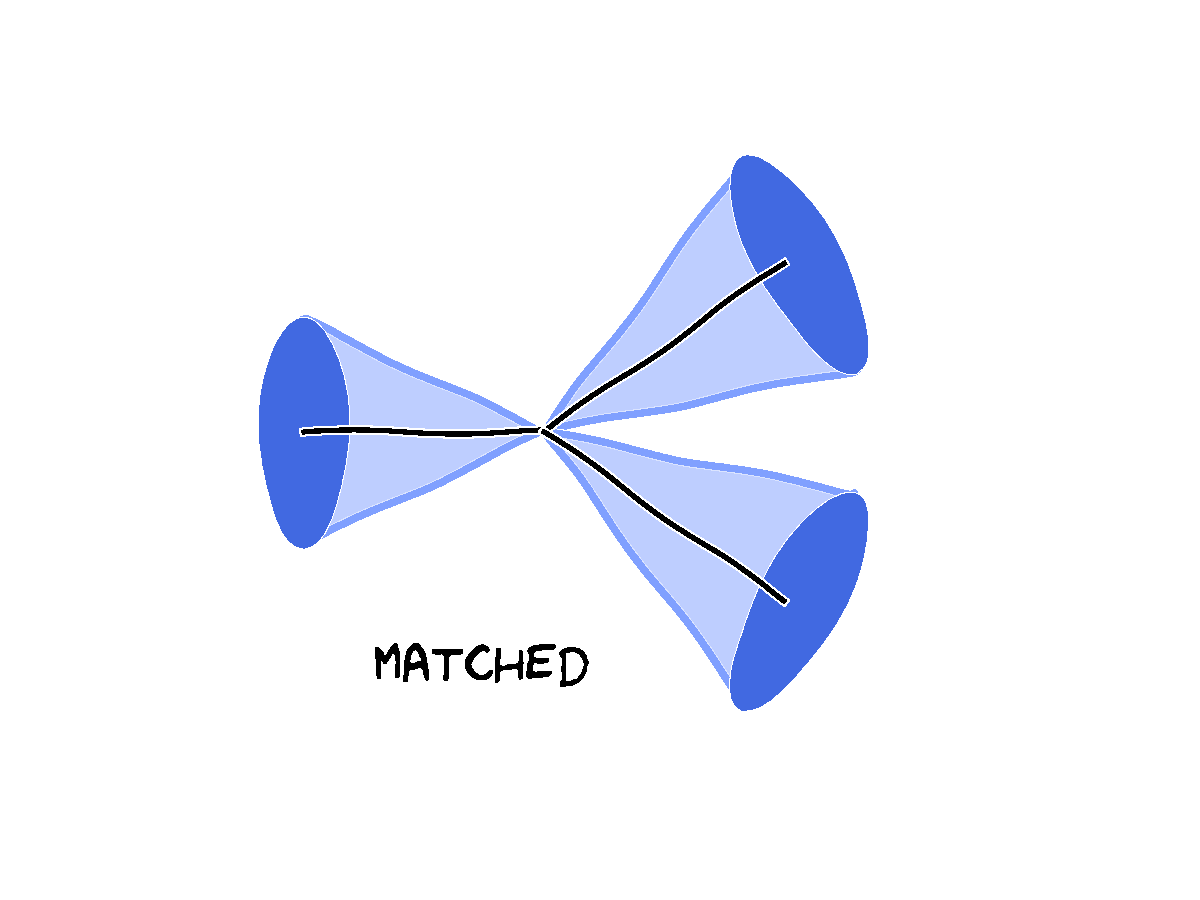
\includegraphics[width=0.31\textwidth, clip=true, trim=4cm 3cm 4cm 2cm]
  {figures/eventreco_generation/matching1}
  ~
  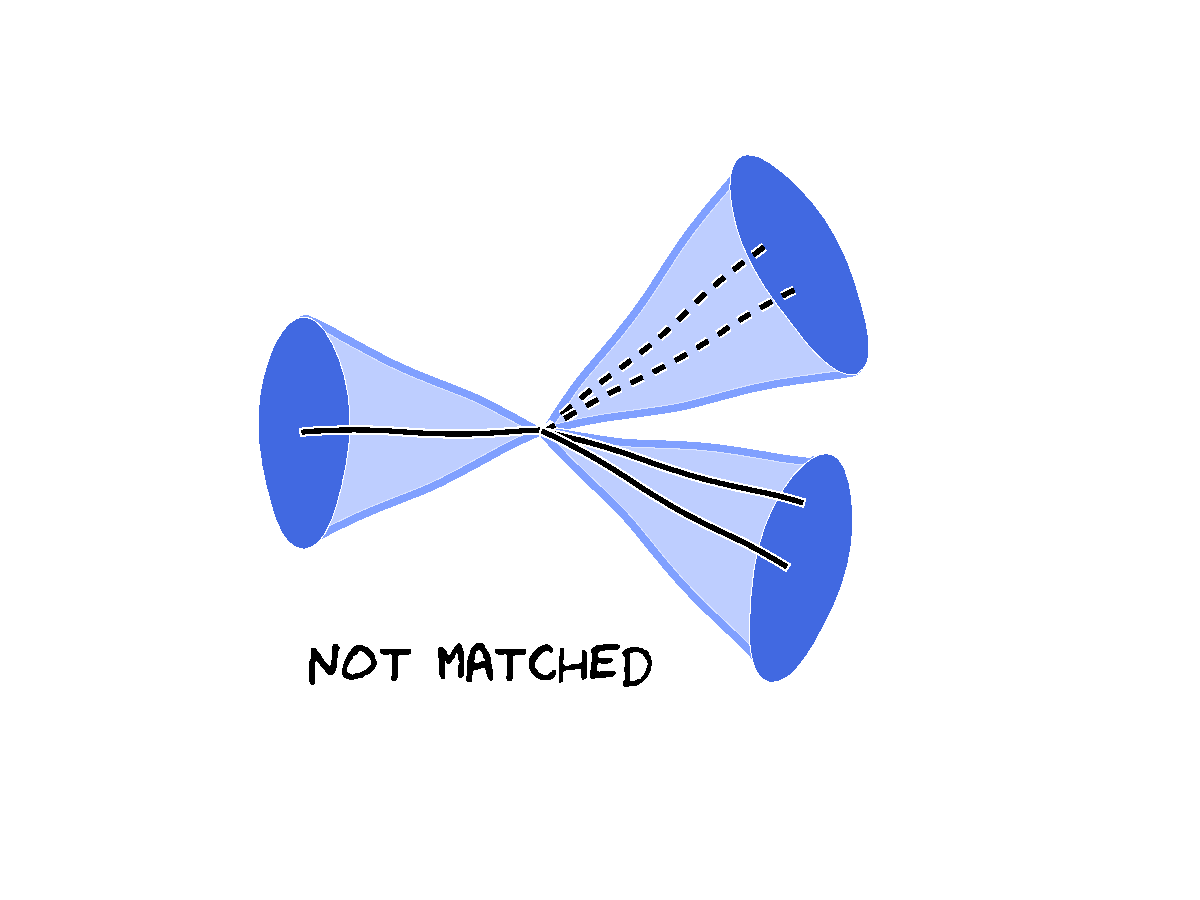
\includegraphics[width=0.31\textwidth, clip=true, trim=4cm 3cm 4cm 2cm]
  {figures/eventreco_generation/matching2}
  ~
  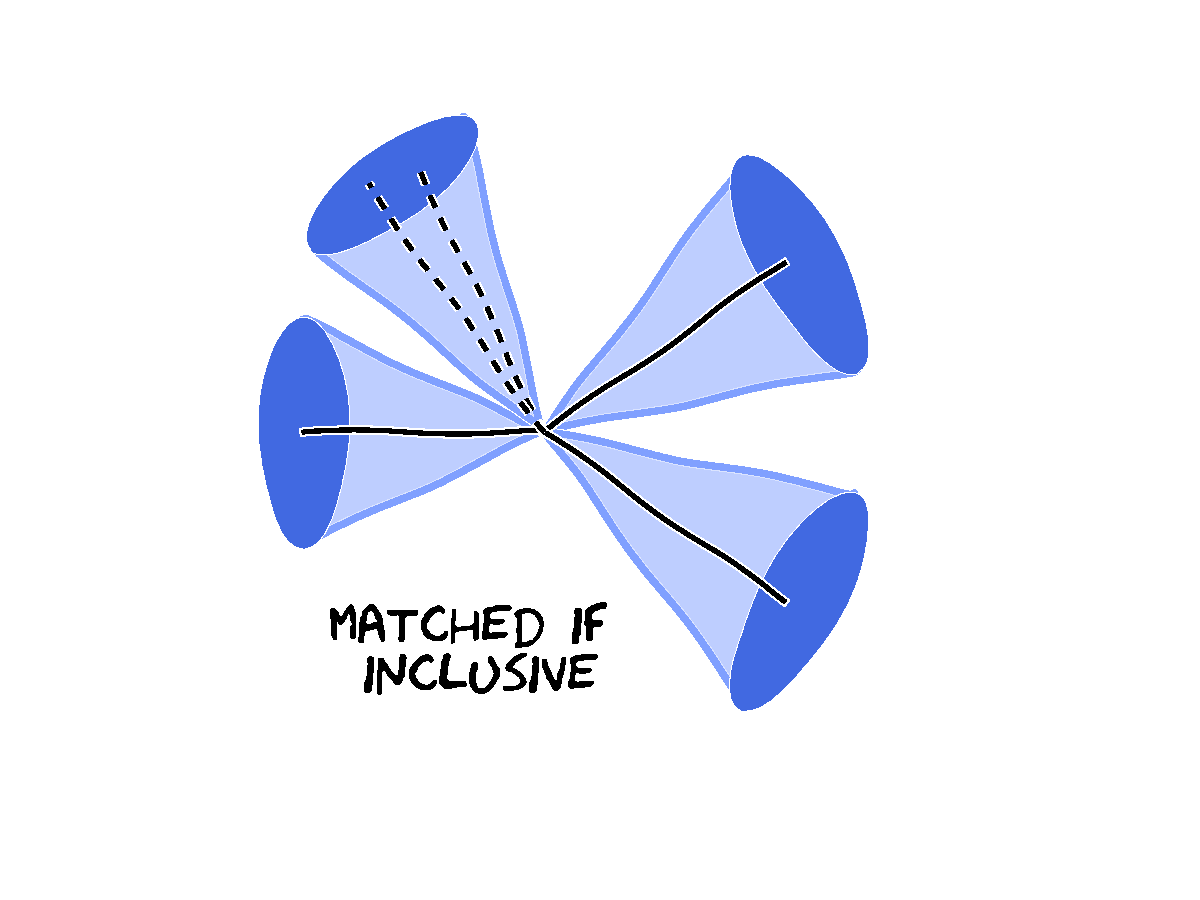
\includegraphics[width=0.31\textwidth, clip=true, trim=4cm 3cm 4cm 2cm]
  {figures/eventreco_generation/matching3}
  \caption{Illustration of the matching procedure for an event with three hard partons (solid
lines). On the left the jet clustering after the shower results in three jets, that are matched to
the three partons. The full event is thus matched, and accepted. In the middle plot the parton
shower added two extra partons (dashed lines), and the hard partons were emitted closer together.
The jet clustering still results in three jets, but now one hard parton cannot be matched to a jet.
The event will thus be rejected. In the right-hand plot each hard parton is matched to a jet, but
there is an additional jet present. If we are in inclusive mode, the event is accepted, otherwise
it is rejected.  
  Figures adapted from Ref.~\cite{mlm_plots}. 
  \label{fig:matching}}
\end{figure}


It is important to verify that the matching procedure behaves properly. In particular, jet related
quantities should have a smooth shape, without any jumps. The presence of discontinuities indicates
that the scales $Q_{\mathrm{match}}$ and $Q_{\mathrm{cut}}^{\mathrm{ME}}$ are not chosen
correctly to ensure a smooth transition between matrix element and parton shower. The distributions
that are typically checked in this regard are the so-called difference jet rates
(DJR)~\cite{Alwall:2008qv}. 

The differential jet rate $i$ is the scale at which a given configuration with $n\geq i$ hard
partons passes from being reconstructed as an $i$-jet one to being reconstructed as an $(i − 1)$-jet
one. 
In this case, with $k_\mathrm{T}$ jet clustering, the differential jet rates are simply the actual
clustering scales. The $1\rightarrow 0$ differential jet rate (DJR1) is the \pt of the last
remaining jet after clustering. The $2\rightarrow 1$ differential jet rate (DJR2) is the smallest of
the \pt of the second last remaining jet and the $k_\mathrm{T}$ between the second and the first
jet, and so on for the other DJR distributions.

Another test of the matching procedure is the stability of the matched cross section when varying
the matching scale. In general, the systematic uncertainty associated to the matching procedure can
be estimated by varying the matching scale. A common choice is to vary the scale by a factor two up
or down. 


\subsection{Hadronization \label{sec:event_hadronization}}

Real events do not consist of partons but of hadrons. Therefore, the set of post-shower partons
must be transformed into a set of primary hadrons, which can then decay further. 
Hadronization is a non-perturbative transition taking place at the hadronization scale. In the
event generation context this scale is by construction identical to the cutoff (resolution) scale of
the parton shower.
Since we have no idea how to calculate the transition between partons and hadrons from first
principles, event generators use QCD-inspired phenomenological models.
Although non-perturbative QCD is not solved, we do have some knowledge of the properties
that such a solution must have. 
An important result from lattice QCD calculations is that the potential of the colour dipole field
between a charge and an anticharge appears to grow linearly with the separation of the charges, when
the separation is greater than about a femtometer. This is known as \textit{linear confinement}, and
is used as a starting point for the string model of hadronization.
The most widely used model is the Lund model, which is implemented in \PYTHIA.

Let us consider the production of a $\cPq\bar{\cPq}$ pair. As the quarks move apart,
linear confinement implies that a potential
\begin{equation}
  V(r) = \kappa r
\end{equation}
is expected at large distances $r$.  This is exactly the potential describing a
string with tension $\kappa$. We can thus interpret this as a colour flux tube that is being
stretched
between the quark and the antiquark. From hadron mass spectroscopy the string tension is
measured to be about $1\GeV/\unit{fm}$.
As the $\cPq$ and $\bar{\cPq}$ move apart, their kinetic energy is gradually converted to potential
energy, stored in the growing string spanned between them. 
Quark-antiquark fluctuations inside the string field can become real particles by absorbing energy
from the string. The original endpoint charges are then screened from each other and the
string breaks into two separate colour-singlet pieces, $(\cPq \bar{\cPq}) \rightarrow (\cPq
\bar{\cPq}') + (\cPq' \bar{\cPq})$. This process continues until only hadrons remain.
Since the string breaks are causally disconnected, they do not have to be considered in any
specific time-ordered sequence. In the Lund model, the string breaks are generated starting
with the hadrons containing the endpoint quarks, and iterating inwards towards the centre of the
string, alternating randomly between the left- and right-hand sides, allowing a single on-shell
hadron to be split off in each step. An illustration of the colour flux tube and the breakup of the
string system is shown in Fig.~\ref{fig:hadronization_string}.

\begin{figure}[htpb]
  \centering
  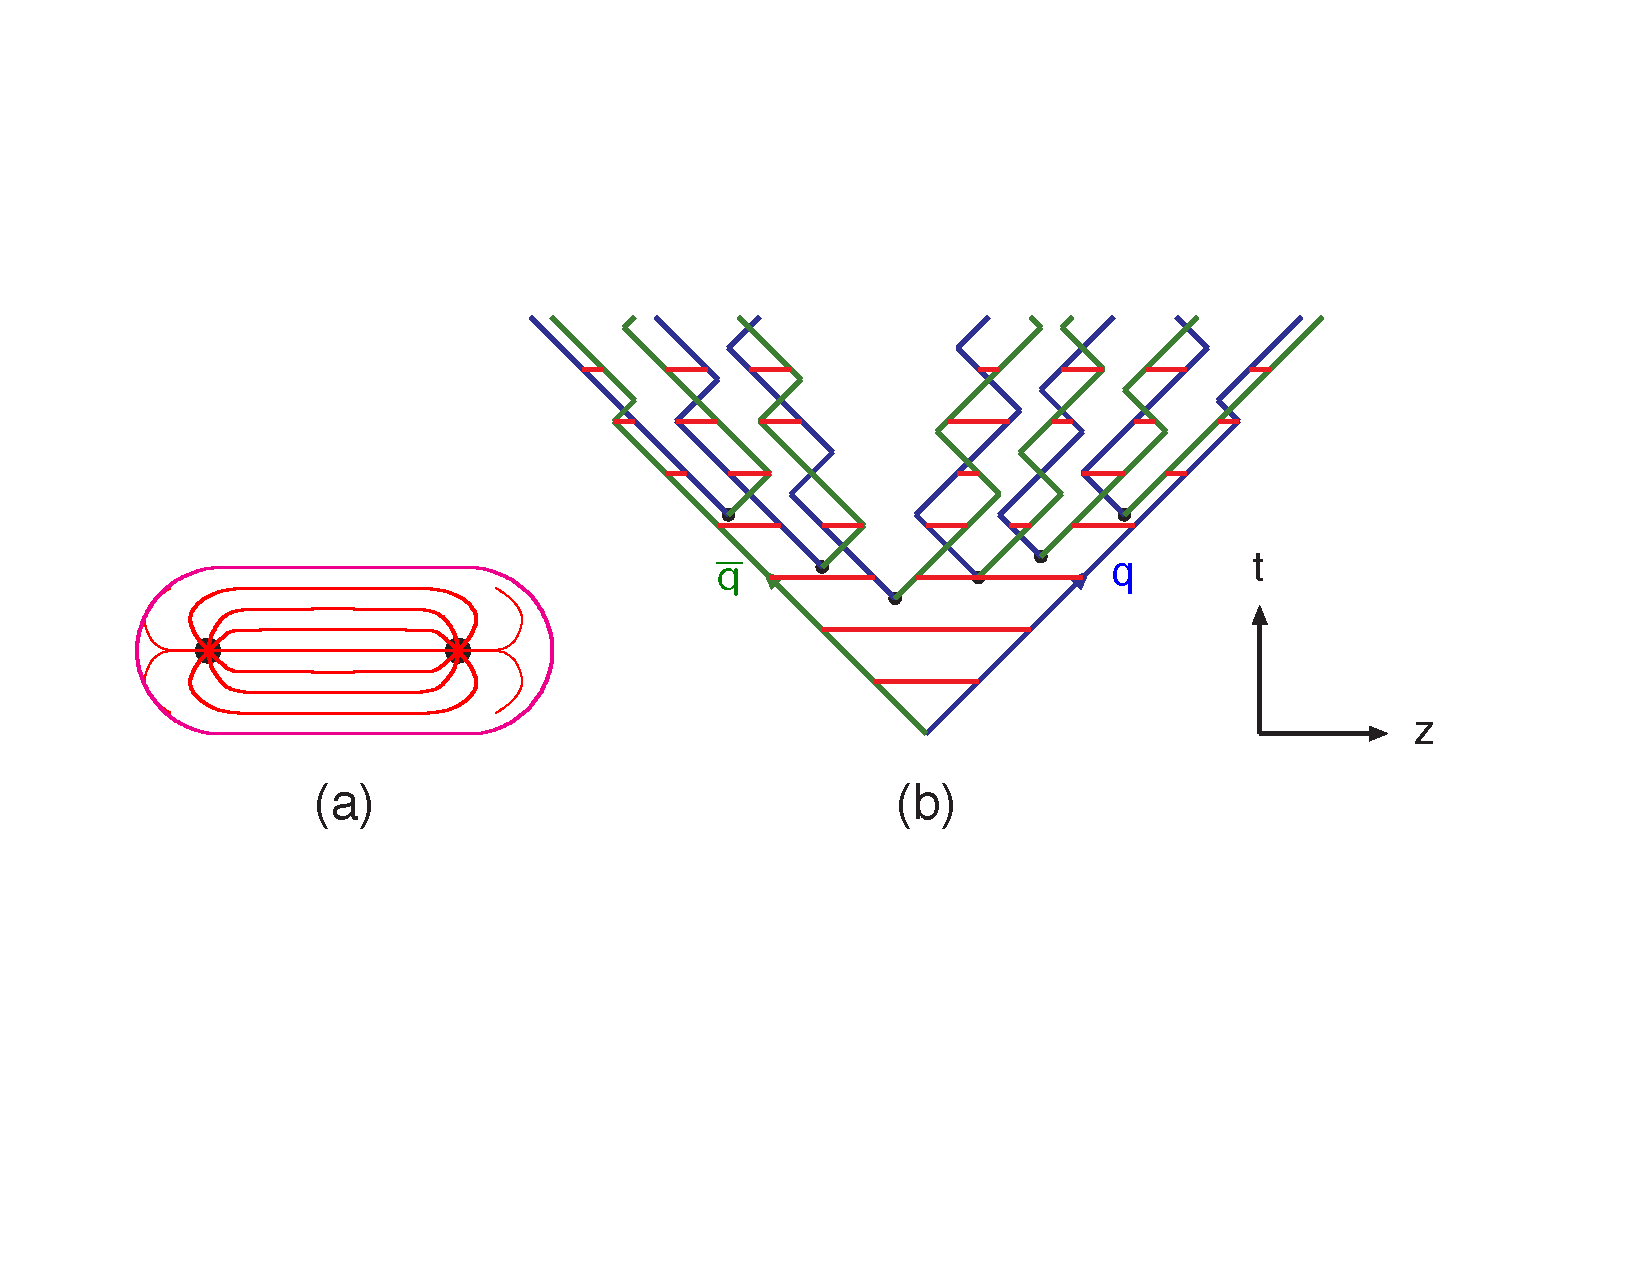
\includegraphics[width=0.8\textwidth]{figures/eventreco_generation/stringone}
  \caption{ (a) A colour flux tube spanned between a quark and an antiquark. (b) The motion
and breakup of a string system. Diagonal lines are (anti-)quarks, horizontal lines snapshots of the
string field. Figure and caption taken from Ref.~\cite{Buckley:2011ms}.
  \label{fig:hadronization_string}}
\end{figure}


The details of the individual string breaks are not known from first principles. The Lund model
uses the idea of quantum mechanical tunnelling, which leads to a flavour-independent
Gaussian spectrum for the transverse momentum (w.r.t. the flux tube) of the $\cPq \bar{\cPq}$ pairs.
Baryon production can be incorporated by allowing string breaks to occur by the production of
pairs of so-called diquarks, loosely bound states of two quarks in a colour antitriplet state. 
Because the knowledge of hadronization is incomplete, experimental input is needed to tune many of
the parameters describing the finer details, such as flavour composition, and the ratio of vector to
pseudoscalar mesons. 


\subsection{Generator tuning}

Monte Carlo event generators are able to provide a full picture of collider final states, down to
the level of individual particles. This allows them to be used as theory reference against which
the standard model, or a new physics model, can be tested. The accuracy of the prediction depends
on the chosen observable, and on the sophistication of the generation. 
Apart from including higher order corrections, or using better non-perturbative models, it is also
crucial to constrain the remaining free parameters of the generation models using existing data.
This process is referred to as generator tuning. 

Generator models have a vast array of adjustable parameters, but most of these control relatively
small details. The few exceptions are the value of $\alpha_S$ in the perturbative domain, and the
form of the fragmentation functions that govern the non-perturbative hadronization process. 
Tuning all possible parameters is usually done in a highly factorized way, constraining just a few
parameters at a time using carefully selected experimental data. 
Of course, subsequent steps can alter the agreement obtained in the previous steps. Obtaining a
full generator tune requires several iterations. 
Automated tools have been developed in recent years to reduce the amount of manpower required.
However, the need for expert input cannot be fully removed. 

Different kinds of experimental data are used to constrain different parameters. Tuning of final
state radiation and hadronization is mostly done using LEP and other $e^+ e^-$ data,  which have
the advantage that the initial state does not cause extra complications in the interpretation of jet
related observables. Constraints on initial state radiation are derived primarily from Drell-Yan
events in hadron collisions. 
While performing the generator tuning it is important to realize that for many observables we do
not expect agreement to better than about 5-10\%. We should thus take care not to overtune on one
single observable, but rather aim for an overall adequate performance. 




\chapter{The razor boost analysis \label{chap:razorboost}}

In this chapter the razor boost analysis will be discussed. 
I will first cover the motivation and general strategy of the analysis in 
sections~\ref{sec:boost_motivation} and \ref{sec:boost_strategy}. Then the \textit{razor variables},
which are our most important discriminating variables, will be derived in 
section~\ref{sec:boost_razor}. Section~\ref{sec:boost_wtag} details the technique used to tag highly
boosted $\W$ bosons. The signal and control region selections are listed in
sections~\ref{sec:boost_signal_selection} and \ref{sec:boost_control_selection}. 
The full statistical treatment, with its likelihood based approach, is explained in 
section~\ref{sec:boost_likelihood}. In section~\ref{sec:boost_systematics} the different sources of
systematic uncertainties are discussed, followed by the results of the full background estimation in
section~\ref{sec:boost_results}. This chapter concludes, in section~\ref{sec:boost_interpretation},
with the interpretation of the results in terms of several simplified model spectra. 

\section{Motivation \label{sec:boost_motivation}}

%%%%%%%%%%%%%%%%%%%%%%%%%%%%
%% Razor boost motivation %%
%%%%%%%%%%%%%%%%%%%%%%%%%%%%

% put text from note and expand.
% look at emails from Harrison and Maurizio

The CERN LHC (Chapter~\ref{chap:LHC}) has provided data sufficient to conduct a large variety of
searches for physics beyond the standard model.
As explained in Chapters~\ref{chap:beyond_standard_model} and \ref{chap:supersymmetry},
supersymmetry is among the best-motivated candidates for new physics and predicts the existence of
supersymmetric partners for each of the standard model particles.  
Scenarios with non-degenerate supersymmetric particle spectra, with cross sections as low as
${\sim}1$~fb, have been explored in many final states~\cite{CMS-PAS-SUS-13-020}; however, as yet no
traces of new physics have been found.  

Recently, the focus of searches has turned towards natural SUSY, in which the Higgs boson mass can
be stabilized without excessive fine tuning. Natural SUSY requires the existence of a light top
squark, $\stopone$, and a somewhat light gluino, $\tilde{g}$, while accommodating mass scales for
other supersymmetric particles that are beyond the direct reach of current LHC data.  
More detailed information on natural supersymmetry can be found in
Section~\ref{sec:susy_natural_susy}. 
The possibility that the top squark could be light has motivated several searches by the CMS and
ATLAS
collaborations~\cite{Aad:2013ija,Aad:2014qaa,Aad:2014bva,Aad:2014kva,Aad:2014kra,Chatrchyan:2013xna,
Chatrchyan:2013mya,Khachatryan:2014doa} for the direct production of top squarks. The sensitivity of
many of these searches, however, diminishes when the mass of the top squark approaches that of the
lightest SUSY particle (LSP), assumed in the remainder of this thesis to be the lightest neutralino,
$\lsp$. Searches looking specifically for $\stopone \rightarrow t \lsp$ also become less sensitive
when the mass difference, $\Delta m$, between the top squark and the LSP is comparable to the top
quark mass, $m_t$. 
These gaps in the sensitivity are illustrated in Fig.~\ref{fig:boost_story_motivation}, which shows
the general form of the exclusion limits for direct stop production, on the
($m_{\stopone},m_{\lsp}$) plane. 
Let us now examine the three regions, shown on the figure with colored ellipses, where general
searches lack sensitivity, in order to determine why these regions are hard to probe, and whether we
can find a strategy to deal with the issues. 

\begin{figure}[htpb]
  \centering
  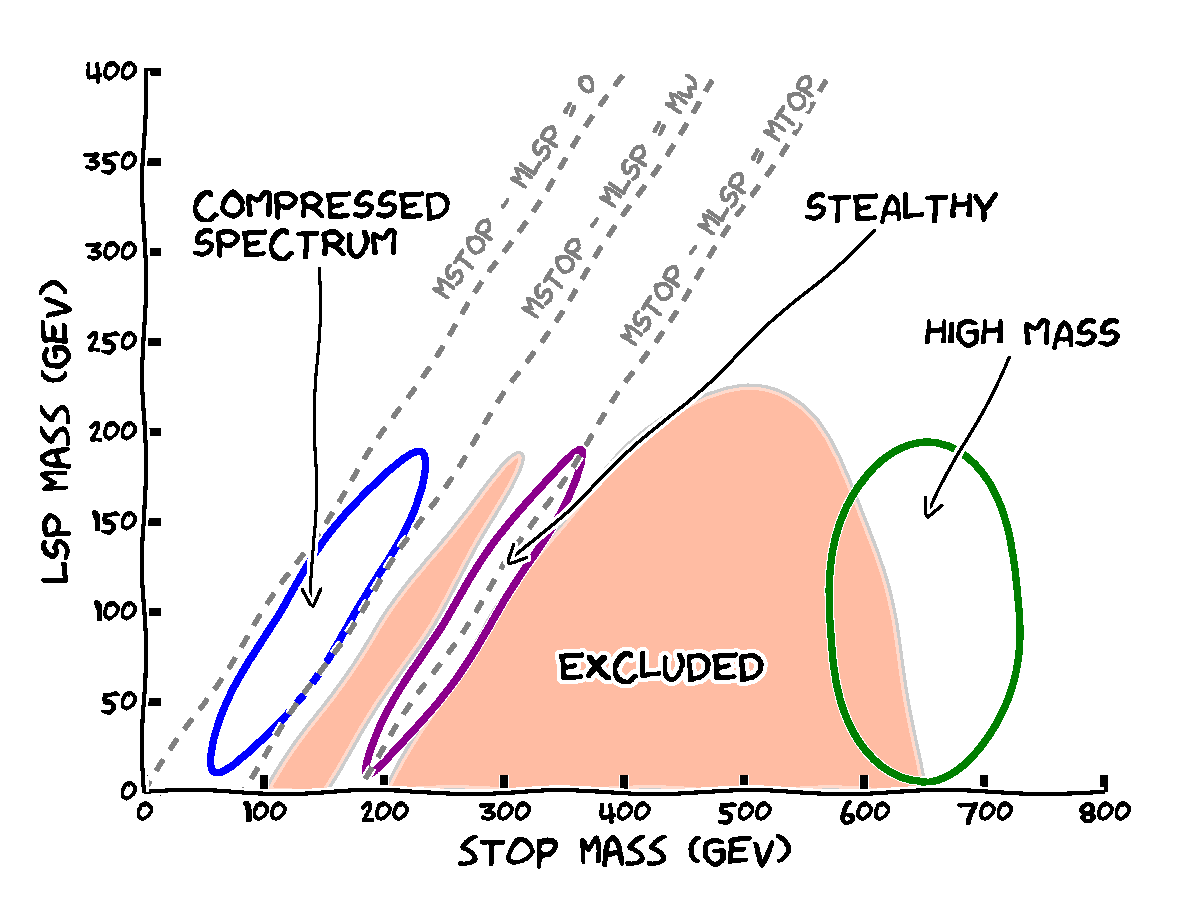
\includegraphics[width=0.8\textwidth]{figures/razor_motivation/story_boost_motivation}
  \caption{General form of the exclusion limits for direct stop production on the
($m_{\stopone},m_{\lsp}$) plane. The red shaded area is the approximate region that has been
excluded by a range of searches. The three colored ellipses indicate the regions that are hard to
probe: the compressed spectra, stealthy top squark scenario and high mass top squarks.
  \label{fig:boost_story_motivation}}
\end{figure}

\paragraph{Compressed scenario}
In general, models with mass spectra featuring small mass splittings are called \textit{compressed
scenarios} or \textit{compressed spectra}. This case thus corresponds to the left-most gap in
Fig.~\ref{fig:boost_story_motivation}, where $\Delta m$ is very small, smaller than the $\W$ boson
mass in particular. 
In this scenario, the top squark decays to the LSP and other soft decay products, either resulting
from the loop-induced decay $\stopone \rightarrow c \lsp$, or from the four-body decay $\stopone
\rightarrow \cPqb f \bar{f} \lsp$. These soft decay products, jets and/or leptons, are difficult to
detect. They are hard to reconstruct, and when reconstructed they often fall below the \pt
thresholds that define the objects. 
Therefore, in order to be sensitive to such processes, one should not rely on the presence of
these objects, but rather on something else, such as the presence of jets from initial state
radiation (ISR). Both ATLAS and CMS have performed searches using this
technique~\cite{CMS-PAS-SUS-13-009,Aad:2014nra}. 

\paragraph{Stealthy stop scenario}
The scenarios where $\Delta m\,{\approx}\, m_t$, are often referred to as \textit{stealthy}
scenarios. The reason for this is that when $\Delta m$ approaches the top mass, the signature of
top squark production is very similar to that of standard model $t\bar{t}$ production,
which has a much higher cross section. Consequently, the signal from direct stop production is
hidden underneath a much larger $t\bar{t}$ background. An alternate way to approach stealthy stops
is, for instance, to assume that the heavy top squark $\stoptwo$ is also accessible at the LHC, and
decays to the $\stopone$ via either a Higgs or $\cPZ$ boson~\cite{Khachatryan:2014doa}. This
results in a longer decay chain, which provides extra handles, such as additional $\cPqb$ quarks or
leptons. 

\paragraph{High mass scenario}
The last gap that is present in the sensitivity of searches for the direct production of top squark
pairs, is the high mass region. In this region the signature is actually very striking, with
usually large hadronic activity and/or missing transverse momentum. The problem lies in the rather
low expected cross section for direct stop production at 8\TeV. We would need much more data than
the $20\fbinv$ that is available to detect this process. 
Of course, with the restart of the LHC at 13\TeV centre-of-mass energy fast approaching, we can
expect to close part of this gap very soon.

\paragraph{}
Apart from the approaches mentioned above, there is another option to tackle the compressed and
stealthy scenarios, namely, looking for top squarks in gluino decays. This is exactly the focus of
the razor boost analysis. 
Specifically, we consider gluino pair production in which the gluino decays to a top squark and a
top quark, $\tilde{g} \rightarrow t \stopone$. In the models considered, largely motivated by
natural supersymmetry, the gluino has a mass around 1-1.5 \TeV and the lighter top squark has a mass
of a few hundred \GeV. Owing to the significant mass gap presumed to exist between the gluino and
the top squark, the top quark from the gluino to top squark decay will receive a large boost.  
The top squark then decays to $c \lsp$ for small $\Delta m$, or to $t \lsp$ for $\Delta m
\,{\approx}\, m_t$. Four-body decays of the top squark are not considered here. 

The simplified models (see Section~\ref{sec:susy_sms} for more information) corresponding to the
decays $\tilde{g} \rightarrow t \stopone$, followed by either $\stopone \rightarrow c \lsp$ or
$\stopone \rightarrow t \lsp$, are called \textit{T1ttcc} and \textit{T1t1t}, respectively, and
illustrated in the diagrams in Fig.~\ref{fig:T1ttcc_T1t1t_diagrams}. For comparison we show in
Fig.~\ref{fig:T2tt_diagram} the diagram for the \textit{T2tt} simplified model, corresponding to
direct top squark production in which the top squark decays to $t \lsp$. 

As the analysis described in this thesis is the first analysis within CMS to explicitely probe
gluino-mediated production of top squark pairs decaying as $\stopone \rightarrow c \lsp$, it
provides new information about the viability of natural SUSY. 

\begin{figure}
  \centering
  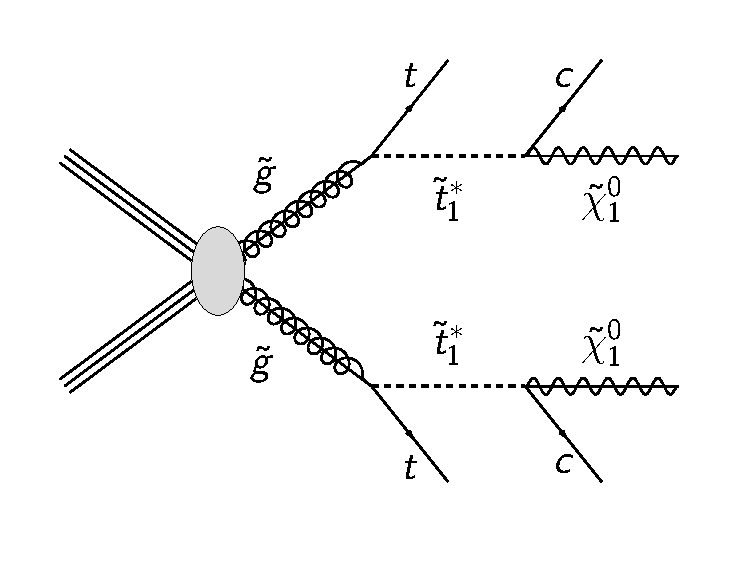
\includegraphics[width=0.48\textwidth,clip=true,trim=0 0.7cm 0 0]
{figures/razor_interpretation/T1ttcc}
  ~
  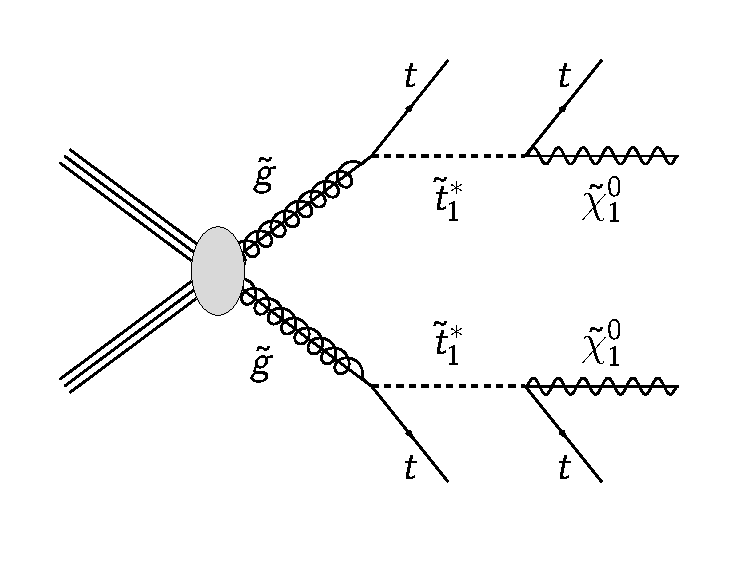
\includegraphics[width=0.48\textwidth,clip=true,trim=0 0.7cm 0 0]
{figures/razor_interpretation/T1t1t}
  \caption{Diagram illustrating the T1ttcc (left) and T1t1t (right) simplified models.
  \label{fig:T1ttcc_T1t1t_diagrams}}
\end{figure}

\begin{figure}
  \centering
  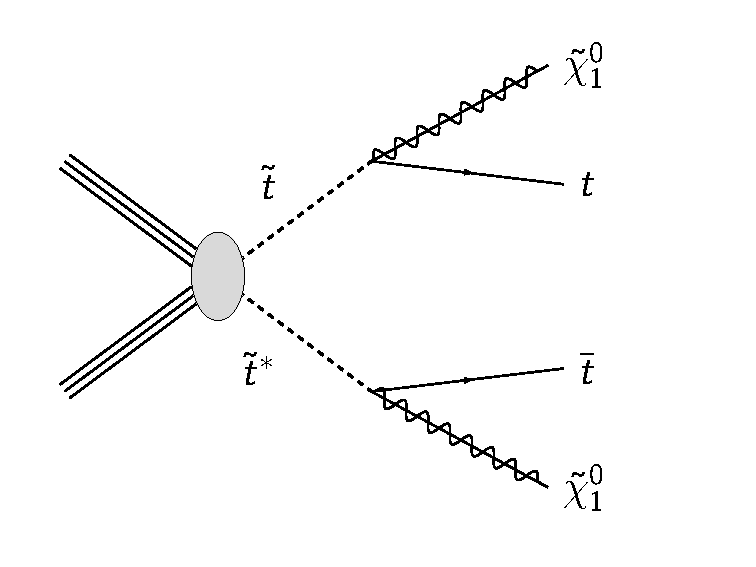
\includegraphics[width=0.48\textwidth,clip=true,trim=0 0.7cm 0 0]{figures/razor_motivation/T2tt}
  \caption{Diagram illustrating the T2tt simplified model.
  \label{fig:T2tt_diagram}}
\end{figure}




\section{General strategy \label{sec:boost_strategy}}

% control regions, transfer factors
% binning in razor variables
% statistical treatment and systematic uncertainties


In light of the discussion in Section~\ref{sec:boost_motivation}, it is expected that boosted top
quarks are a promising signature of new physics involving a massive gluino decaying to a relatively
light top squark.
Boosted objects with high transverse momentum are characterized by merged decay products
separated by $ \Delta R \,{\sim}\, 2m/\pt$\footnote{Considering a heavy object $\W$ with mass $M$
that decays to two massless particles $a$ and $b$, we find $M^2 = 2 p_a \cdot p_b = 2 E_a E_b (1
- \cos{\theta_{ab}})$. Using small angle approximation this becomes $M^2 = E_a E_b
\theta_{ab}^2$. Assigning half of the $\W$ energy to both $a$ and $b$ results in $M^2 =
\frac{1}{4} E_\W^2 \theta_{ab}^2$. Translating this relation into the transverse plane, we get
$\Delta R = \frac{2 M}{\pt^\W}$.}, 
where $m$ and $\pt$ denote the mass and transverse momentum of the mother particle, and $\Delta R$
is given in terms of azimuthal angle $\phi$ and pseudorapidity $\eta$ as $\Delta R = \sqrt{\Delta
\phi^2 + \Delta \eta^2}$.
For a separation of $\Delta R = 0.5$, a top quark should thus have a momentum of ${\sim}700$\GeV, a
value difficult to reach with proton-proton collisions at 8 TeV. Therefore, in order to increase the
signal efficiency, we consider instead $\W$ bosons from top quark decays, which are required to have
a more accessible $\pt \,{\sim}\, 320$\GeV.  The \pt of the top quark and $\W$ boson at generator
level without applying any selection, is shown in Figs.~\ref{fig:boost_gen_toppt} and
\ref{fig:boost_gen_Wpt} for several signal models, and the SM $t\bar{t}$ process. 
We observe that the average \pt is higher for the signal than for $t\bar{t}$. Requiring the
presence of a boosted $\W$ boson will thus be part of the strategy to reduce the SM background.
Hadronically decaying boosted $\W$ boson candidates will be identified using pruned jet
mass~\cite{Ellis:2009su,Ellis:2009me,Chatrchyan:2013vbb} and a jet substructure observable
called N-subjettiness \cite{Thaler:2010tr}. More details on the $\W$ tagging technique will be given
in Section~\ref{sec:boost_wtag}. 

\begin{figure}[htpb]
\centering
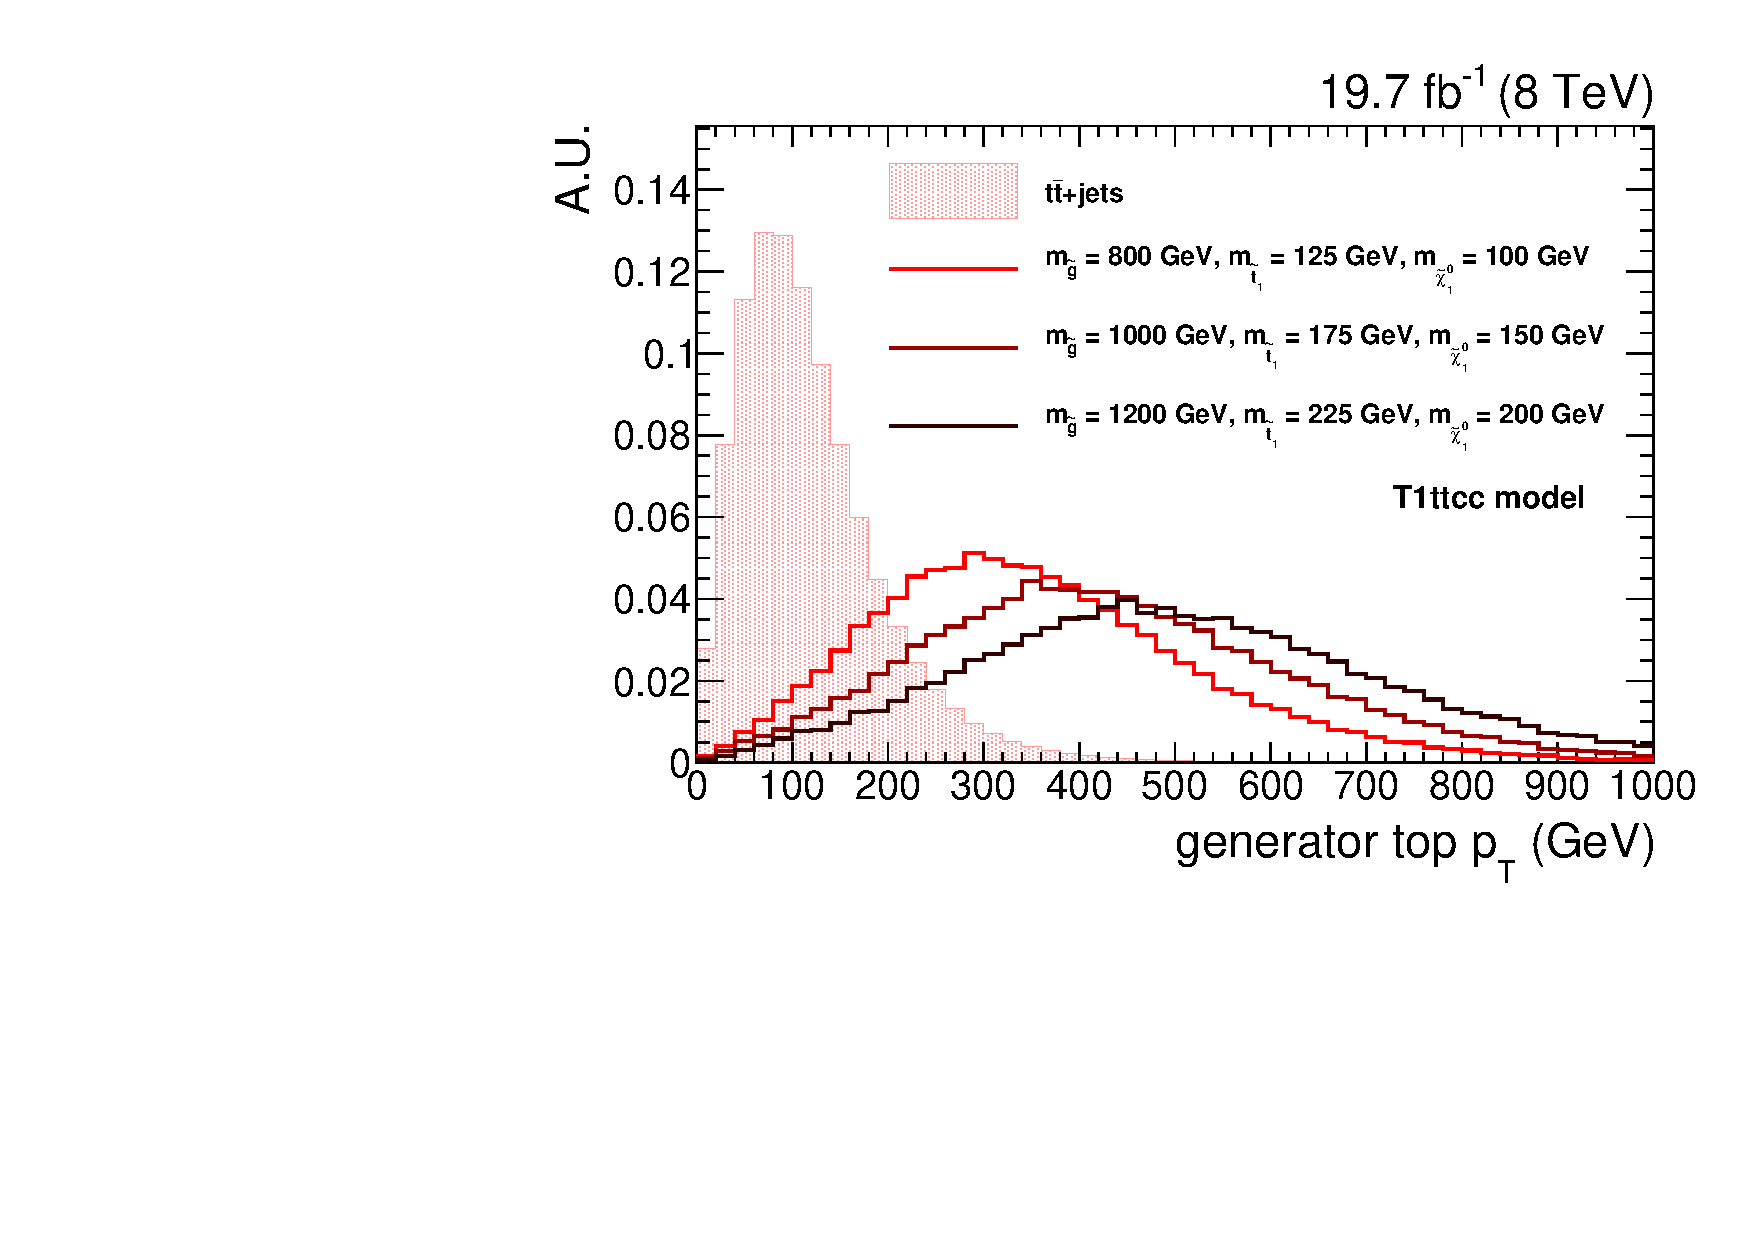
\includegraphics[width=0.48\textwidth]{figures/razor_strategy/T1ttcc_gentoppt}
~
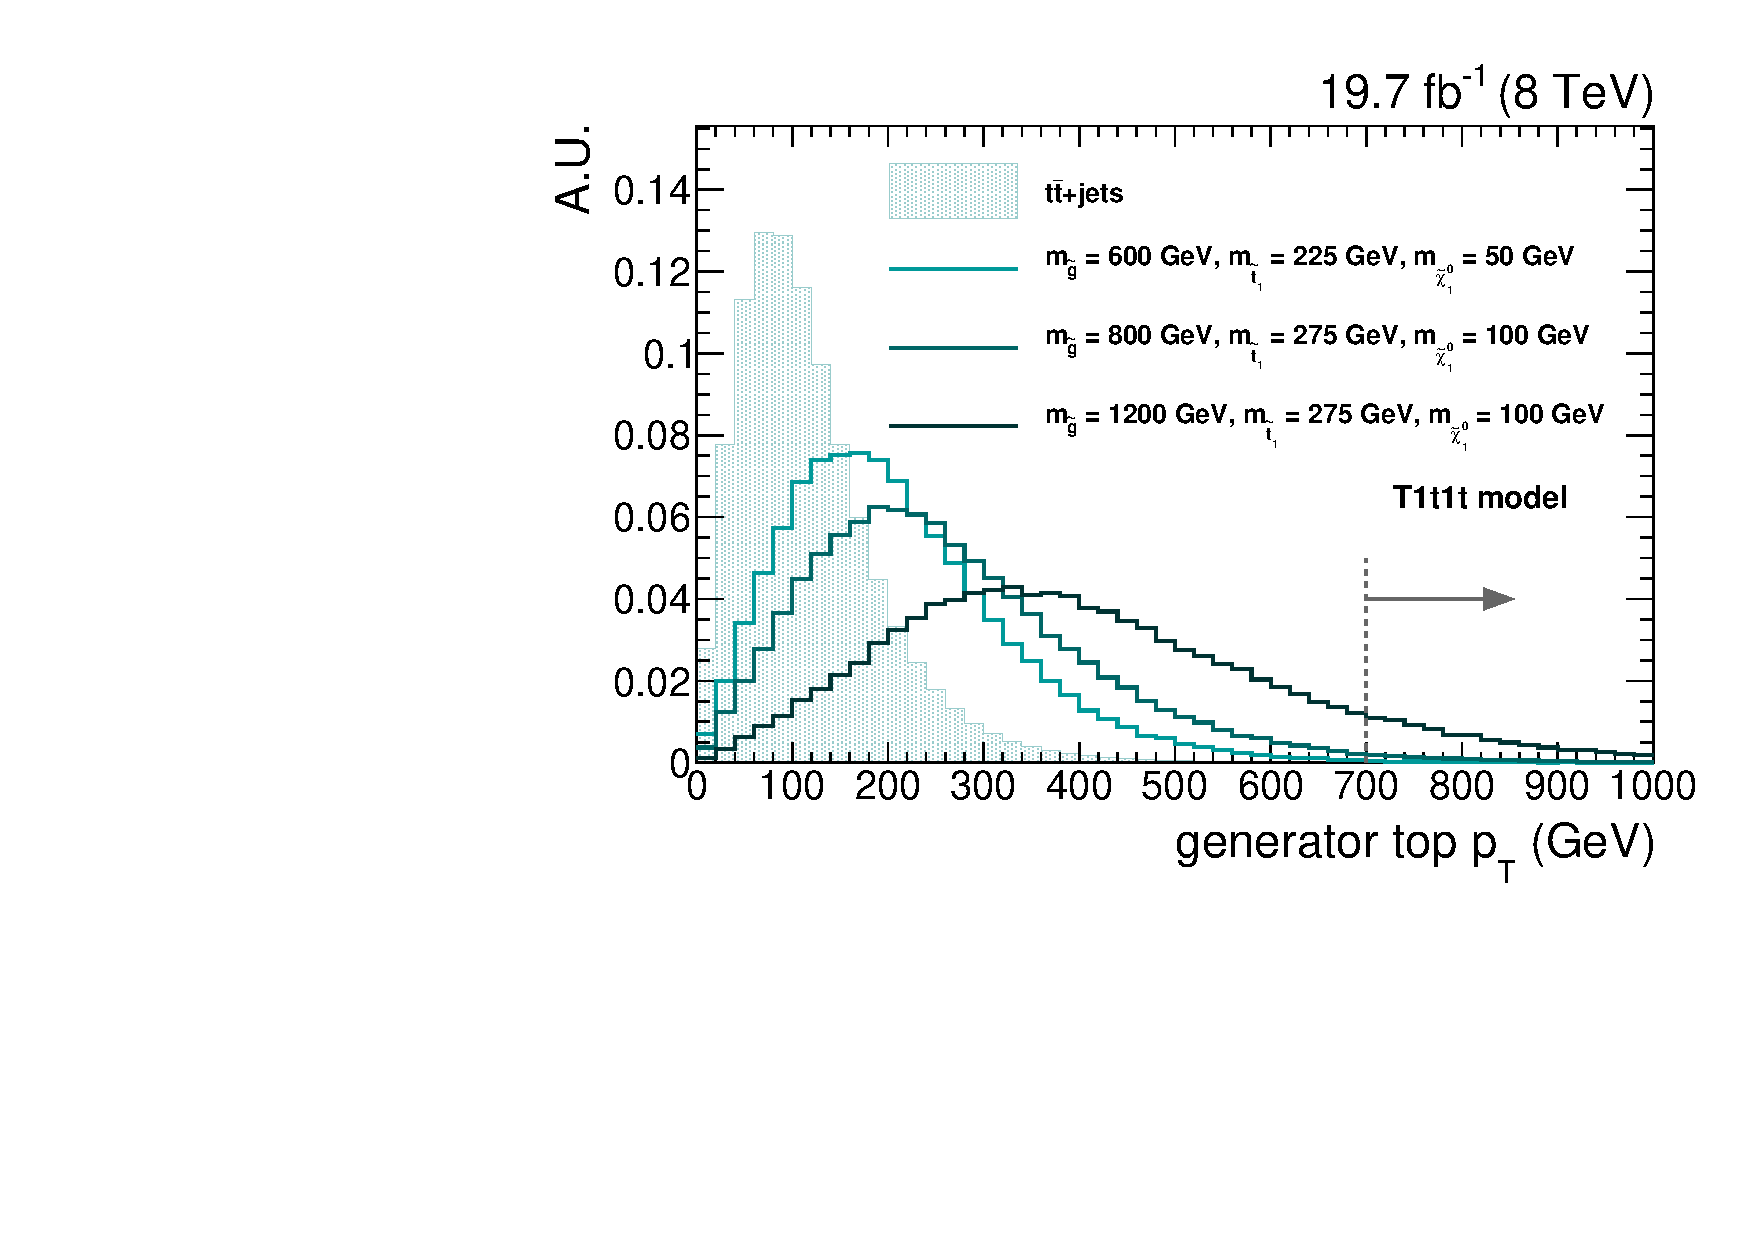
\includegraphics[width=0.48\textwidth]{figures/razor_strategy/T1t1t_gentoppt}
\caption{Generator level top quark \pt for several signal points of the T1ttcc (left) and T1t1t
(right) simplified models. The average \pt increases as the mass splitting increases. The boost of
the top quark is larger for the considered signal models compared to the $t\bar{t}$ background. 
\label{fig:boost_gen_toppt}}
\end{figure}
\begin{figure}[htpb]
\centering
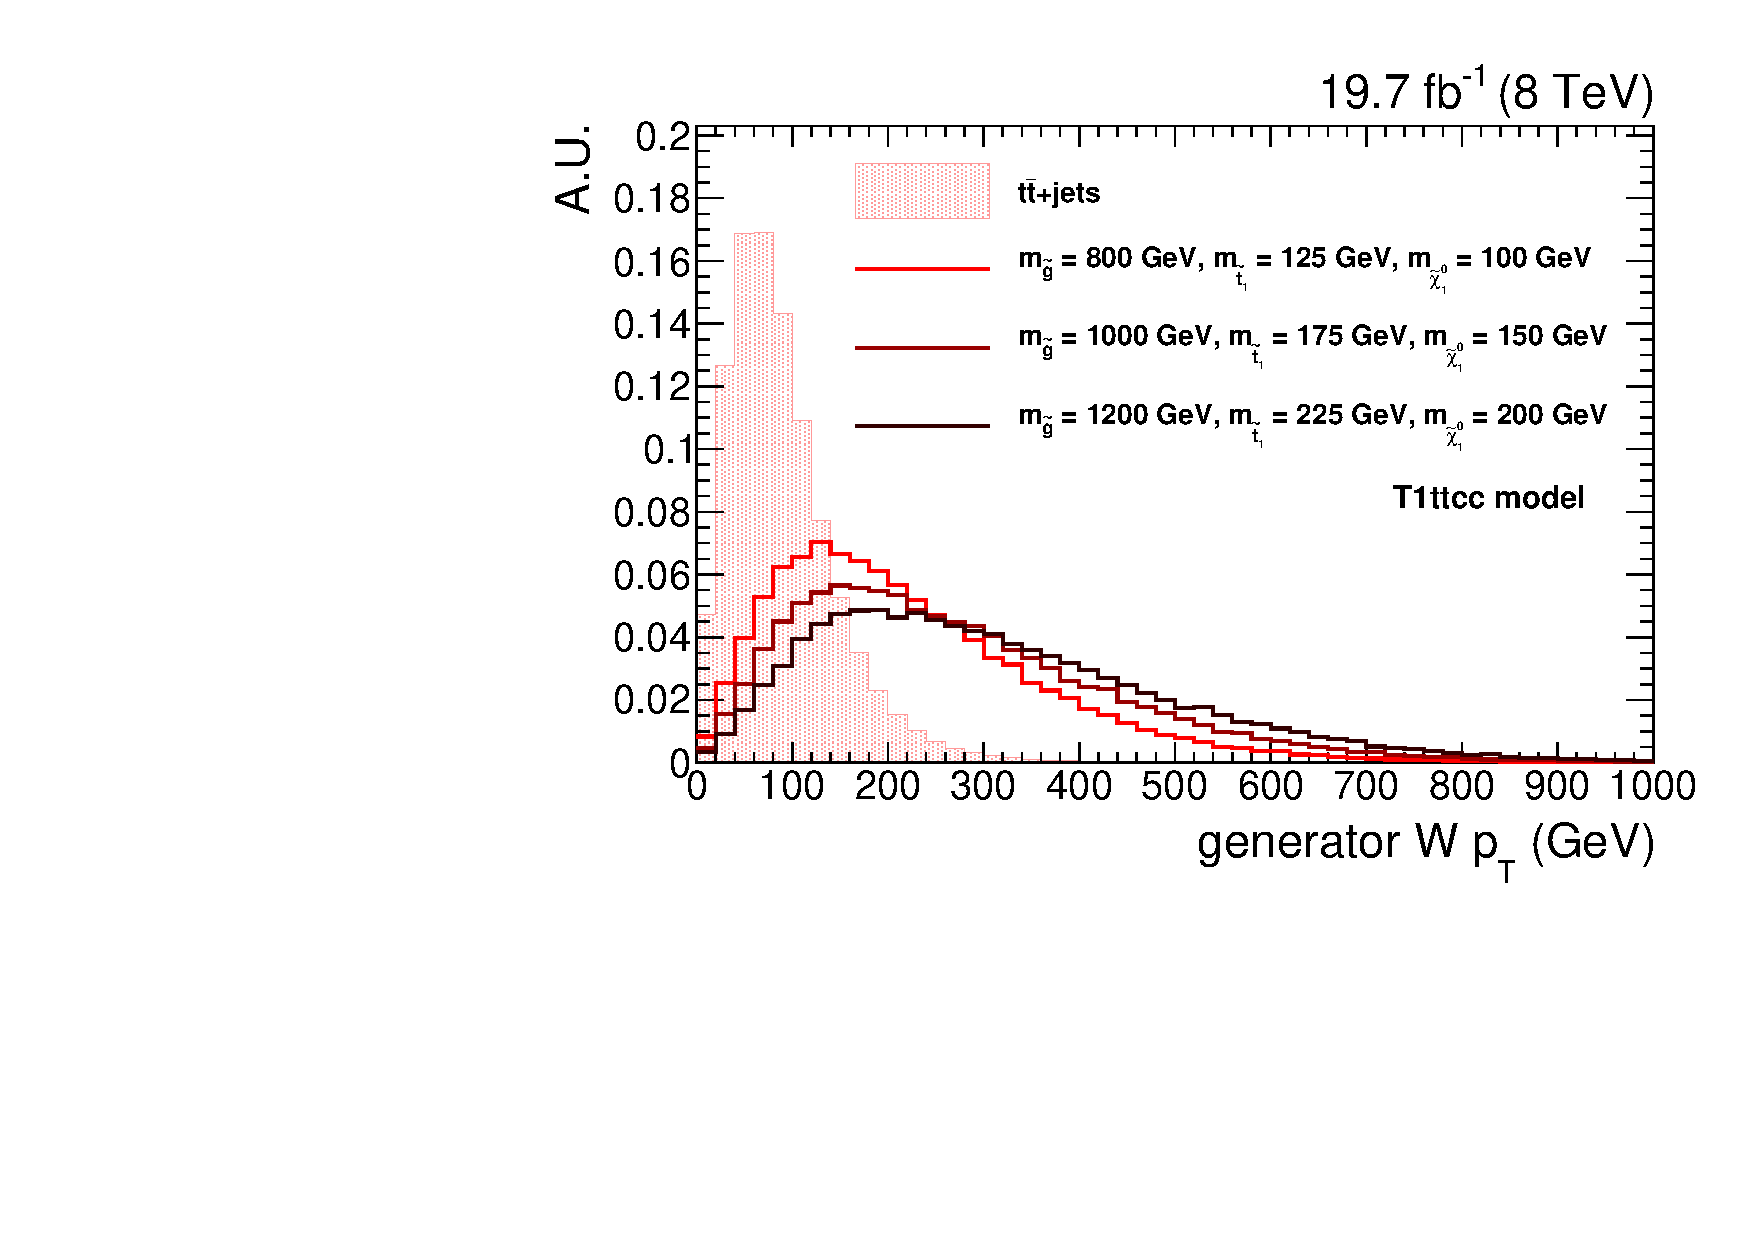
\includegraphics[width=0.48\textwidth]{figures/razor_strategy/T1ttcc_genWpt}
~
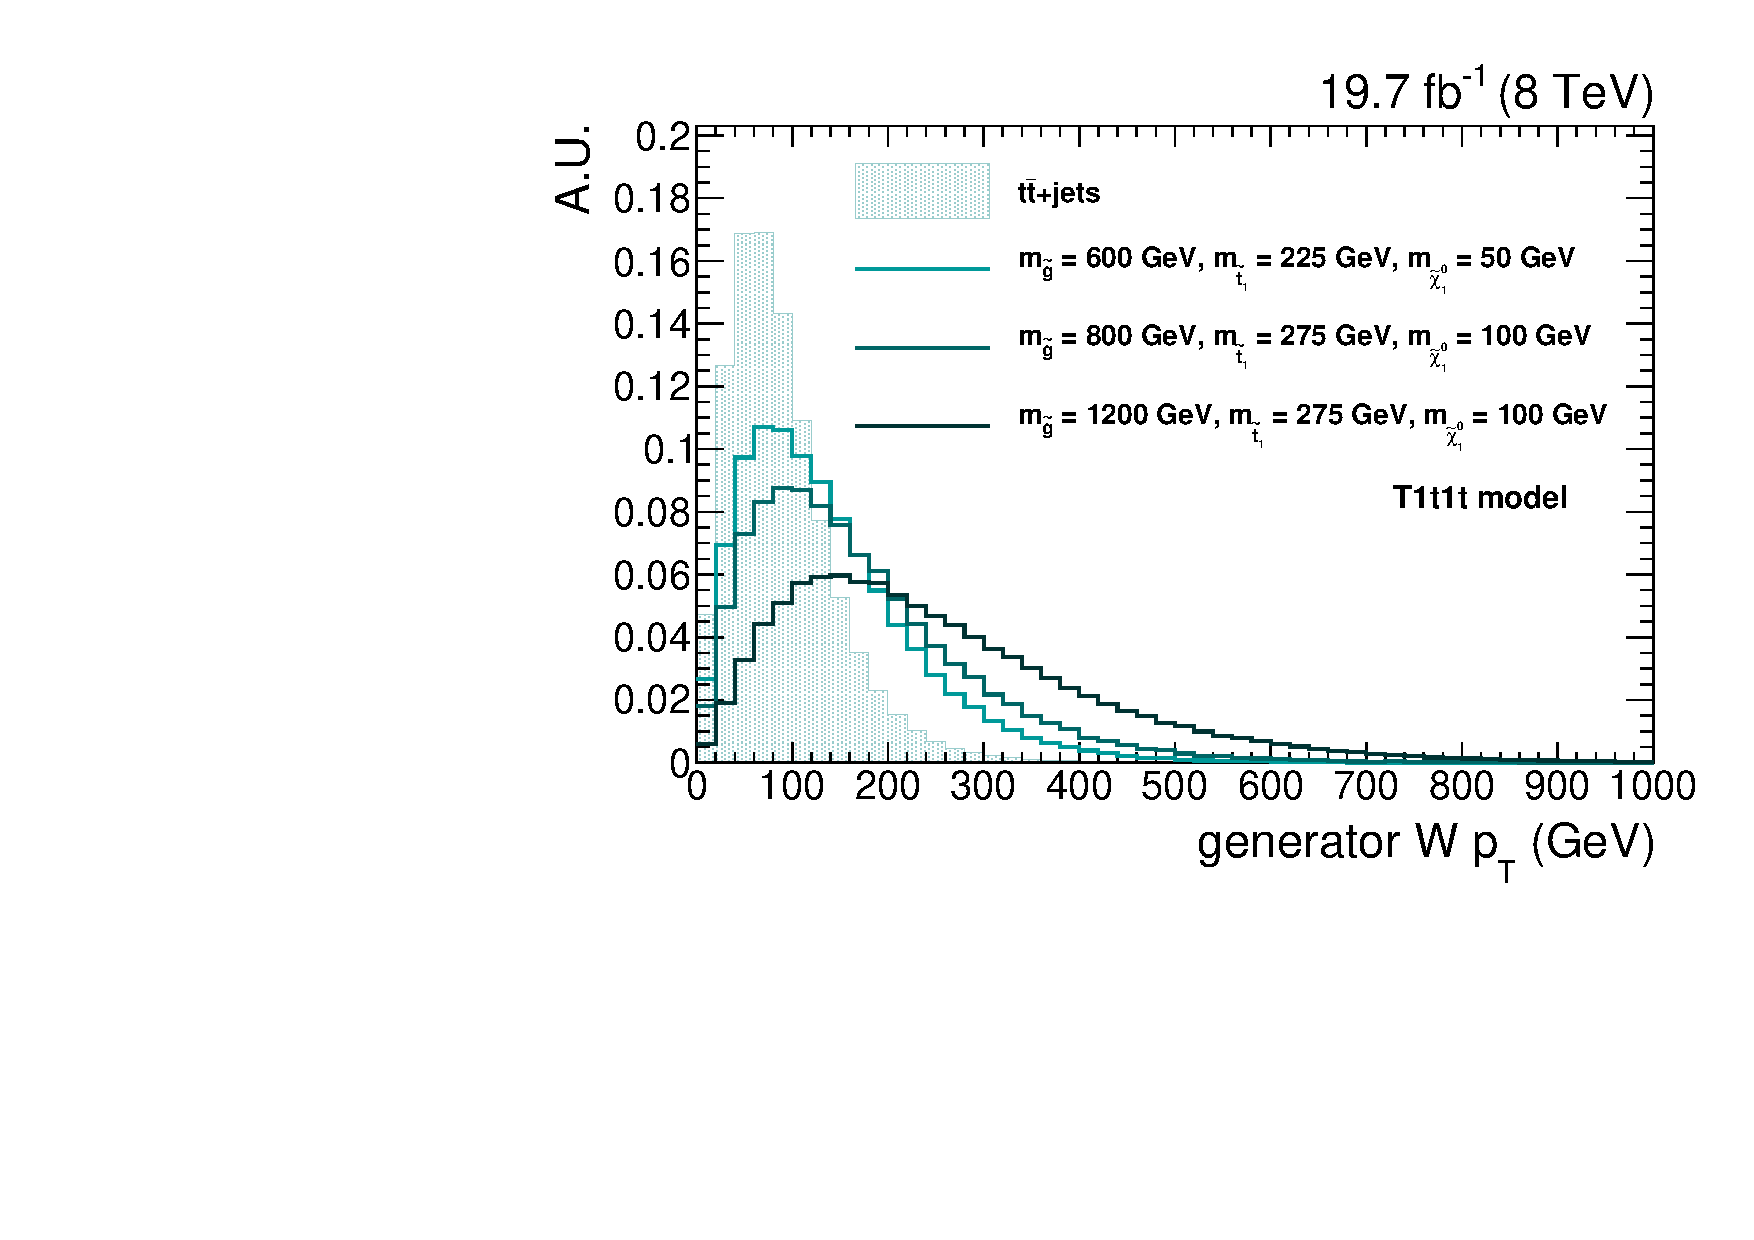
\includegraphics[width=0.48\textwidth]{figures/razor_strategy/T1t1t_genWpt}
\caption{Generator level $\W$ boson \pt for several signal points of the T1ttcc (left) and T1t1t
(right)
simplified models. The average \pt increases as the mass splitting increases. The boost of the $\W$
boson is larger for the considered signal models compared to the $t\bar{t}$ background. 
\label{fig:boost_gen_Wpt}}
\end{figure}

The razor kinematic variables \mr and \rsq, see Section~\ref{sec:boost_razor}, are designed to
discriminate processes with new heavy particles and missing energy from standard model processes.
They will be used in this analysis as the main discriminating variables to search for deviations
from the SM. We will perform the search in 25 search bins across the high $\mr$-high $\rsq$ region,
using hadronic events with at least one boosted $\W$ boson and one jet originating from a $\cPqb$
quark (i.e. $\cPqb$ jet). 

Standard model backgrounds in the signal regions are estimated using observations in control regions
and global scale factors, calculated from simulated data, that relate the number of events in one
region to that in another. 
Three control regions, $Q$, $W$, and $T$, are defined to select high-purity samples of multijet,
$\W(\rightarrow \ell\nu)+$jets and $t\bar{t}$ processes, respectively.  
The background estimation method uses a likelihood-based approach, with a simultaneous sampling
of systematic uncertainties which fully takes into account any correlations automatically.
An overview of the different regions and how they are related, including for the control regions
which background parameters of the likelihood each region constrains, is shown in
Fig.~\ref{fig:boost_flowchart}. For the full explanation of the background estimation method, I
refer to Section~\ref{sec:boost_likelihood}. 

\begin{figure}[p]
  \centering
  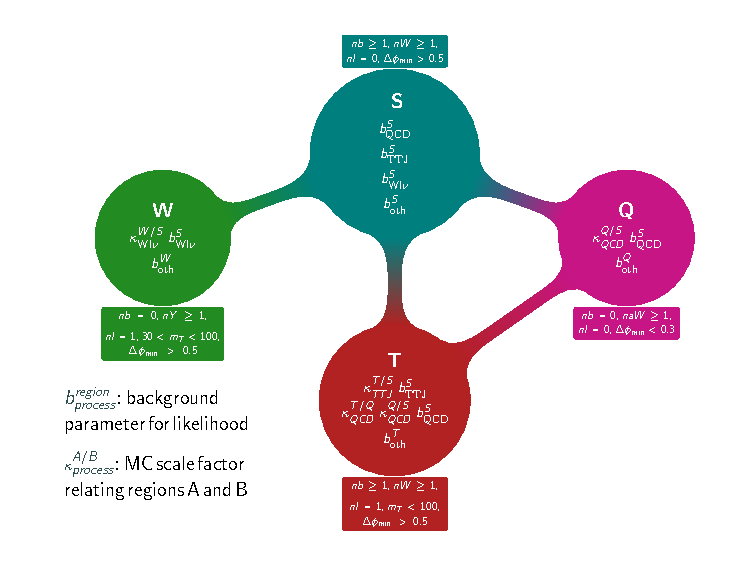
\includegraphics[width=\textwidth]{figures/razor_strategy/BoostFlowChart_noZ}
  \caption{Definition of, and relationship between, the signal ($S$) and control ($Q,T,W$) regions
and their relationship to the bin-by-bin background parameters
$b^{\textrm{region}}_{\textrm{process}}$ for a given region and background process, as well as the
four global scale factors $\kappa^{A/B}_{\textrm{process}} = \sum_i b^A_{\textrm{process}, MC, i} /
\sum_i b^B_{\textrm{process}, MC, i}$, where the sum is over all 25 (\mr,\rsq) bins of the simulated
data. 
The total expected background, per bin, is the sum of the terms shown for each region. Furthermore,
associated with each bin of each region is an observed count $N^{\textrm{region}}$, a simulated
count $N^{\textrm{region}}_{\textrm{process}, MC}$, and a count $N^{\textrm{region}}_{oth, MC}$
equal to the sum of the smaller backgrounds, with associated parameter $b^{\textrm{region}}_{oth}$.
  \label{fig:boost_flowchart}}
\end{figure}

% 
% \begin{figure}[htbp]
% \centering
% \includegraphics[width=0.49\textwidth]{figures/T1ttcc/Signal_comparison_T1ttcc_gen_toppt}
% \includegraphics[width=0.49\textwidth]{figures/T1t1t/Signal_comparison_T1t1t_gen_toppt}
% \caption{Generator top \pt for several signalpoints of the T1ttcc (left) andT1t1t (right)
% simplified
% models.
% \label{fig:gen_toppt}}
% \end{figure}

\section{Razor variables \label{sec:boost_razor}}

%%%%%%%%%%%%%%%%%%%
% razor variables
%%%%%%%%%%%%%%%%%%%

% add full derivation
% plots of signal and background

Many extensions of the Standard Model (see chapter~\ref{chap:beyond_standard_model}) predict the 
existence of new particles, which can be pair-produced in the proton-proton collisions at the LHC. 
Some of those theories introduce an extra symmetry, such as the R-parity in supersymmetry. A
consequence of this symmetry is that the lightest BSM particle must be stable, as it cannot decay
to SM particles only. This lightest BSM particle, called LSP in supersymmetric theories, is weakly
interacting, and escapes the detector unseen. 

This general property leads us to a generic class of new physics signatures in which a heavy
particle is pair-produced, and decays into visible, i.e. interacting with our detector, SM
particles, and an invisible LSP. This signature is illustrated in figure~\ref{fig:razor_signature}.

\begin{figure}[htb]
  \centering
  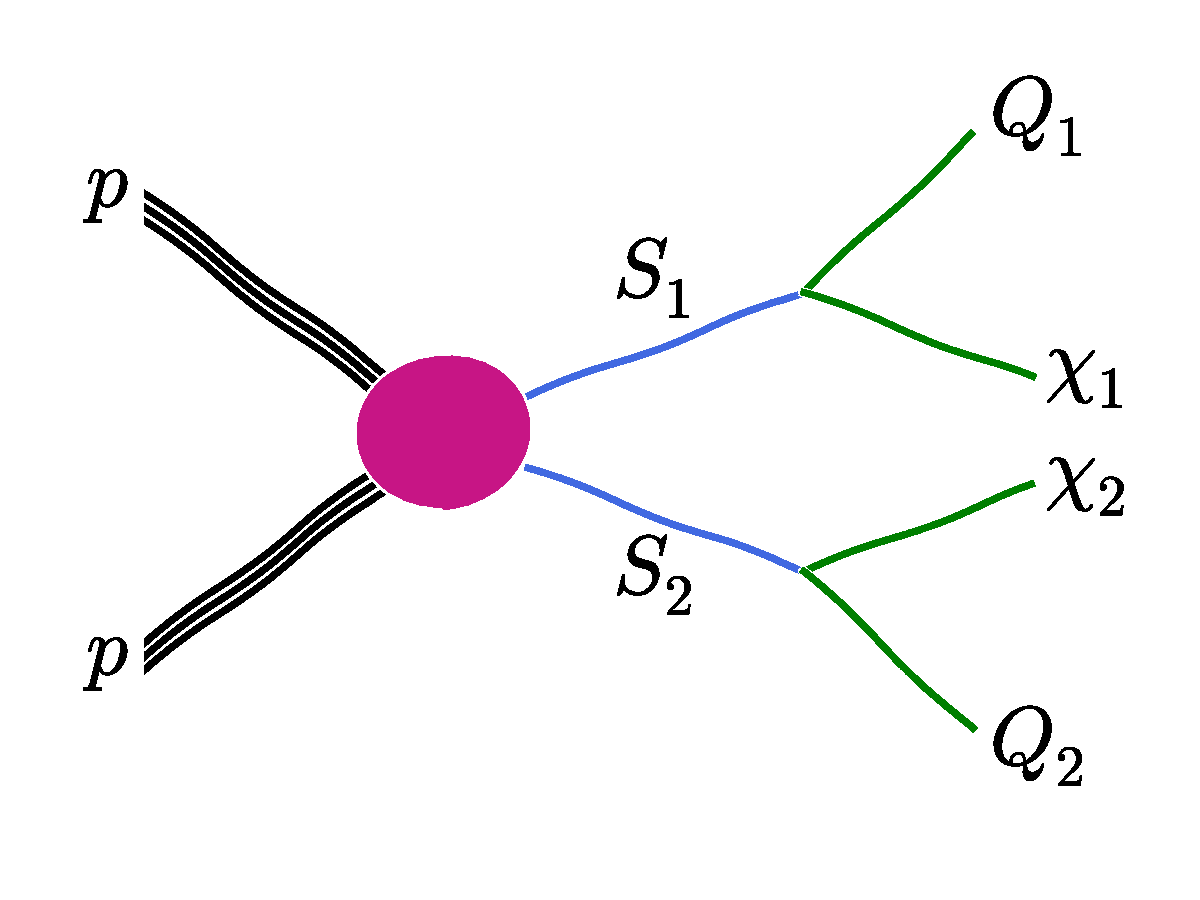
\includegraphics[width=0.6\textwidth,clip=true,trim=0 1.8cm 0
0.8cm]{figures/razor_variables/signature} 
  \caption{Generic new physics signature. Two massive new particles, $S_1$ and $S_2$, are produced
in $\Pp\Pp$ collisions at the LHC, and consequently decay to a visible system $Q_i$ and an invisible
system $\chi_i$. \label{fig:razor_signature}}
\end{figure}

Several kinematical variables targetting this topology have been
developed~\cite{Lester:1999tx,Barr:2003rg,Randall:2008rw,Polesello:2009rn,Bai:2012gs}.
% TODO add citations here
Most of these variables rely on the presence of the invisible LSP's. This causes the visible system
to deviate from a di-jet topology, resulting in possibly large missing transverse momentum, altered
angular distributions, et cetera. All of this can be used to distinguish the sought-after signal
from the known background processes. 
Unfortunately, the ultimate goal of reconstructing the masses of the new particles cannot be
attained. Because of the escaping LSP's, there is simply not enough information available to fully
constrain the problem. What we can do, however, is approximate the mass scale of the new physics
particles. Often times this results in variables that exhibit a kinematic edge. 
The \textit{razor variables} \cite{rogan,Rogan:1557072,Chatrchyan:2011ek,Chatrchyan:2014goa} are no
exception in this regard. One advantage the razor variables have over many other variables, is that
they also reconstruct the mass scale as a peak, in addition to a kinematic edge. 
In what follows I will derive the two razor variables, denoted \mr and \rsq, which use longitudinal
and transverse event information, respectively, to estimate a characteristic mass scale associated
with the new particles. At the end of this section I will briefly show how the razor variables are
used in the razor boost analysis. 

% explain reference frames

\subsection{Kinematical configuration and notation \label{sec:razor_notation}}

Let's again consider figure~\ref{fig:razor_signature}. For simplicity, we will assume that the
produced particles $S_1$ and $S_2$ undergo a two-body decay. Each $S_i$ decays to a visible,
standard model particle $Q_i$, and a particle $\chi_i$ that escapes the detector. 
We assume a symmetric decay chain, with the following relations for the masses of the different
particles,
\begin{alignat}{3}
  M_{S_1} &= M_{S_2} &&= M_S \label{eq:equal_S_masses}\\
  M_{\chi_1} &= M_{\chi_2} &&= M_{\chi} \label{eq:equal_chi_masses}\\
  M_{Q_1} &= M_{Q_2} &&= 0 \label{eq:no_Q_masses}
\end{alignat}

There are four relevant reference frames for our goal of determining a characteristic mass scale
of the new physics process under consideration. The following paragraphs will go through each of
these and define the notations that will be used, as well as deriving relations between several
variables. 

\paragraph{$S_1$ rest frame} 
From basic two-body decay kinematics it follows that the $Q_1$ and $\chi_1$ particles are produced
back to back, with equal magnitude of momentum, in the rest frame of the $S_1$ particle. This is
illustrated in figure~\ref{fig:razor_S1_rest_frame}. 

\begin{figure}[htpb]
  \centering
  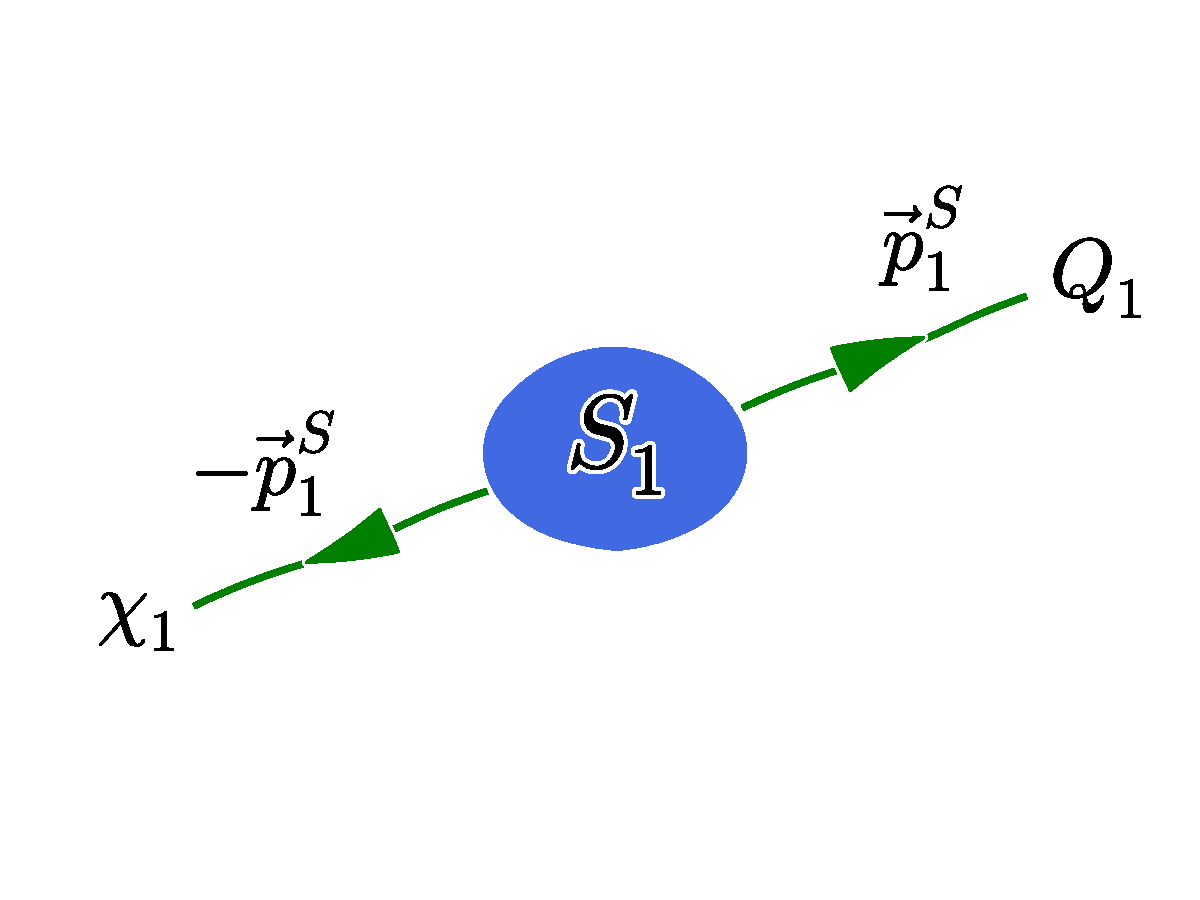
\includegraphics[width=0.6\textwidth,clip=true,trim=0 4cm 0
3cm]{figures/razor_variables/rest_frame}
  \caption{Configuration of the $S_1$ rest frame. The decay products $Q_1$ and $\chi_1$ are
produced back to back with momenta $\vec{p}^S_1$ and $-\vec{p}^S_1$, respectively. 
\label{fig:razor_S1_rest_frame}}
\end{figure}

We can compute the magnitude of this momentum in terms of the new particle masses. To do this we
start from the four-vectors of the $Q_1$ and $\chi_1$ particles in the $S_1$ rest frame, 
\begin{alignat}{6}
  P[Q_1]    &\equiv q_1^S   &&= \{ E^S_{Q_1}, \vec{q}^S_1\} , \\
  P[\chi_1] &\equiv \nu_1^S &&= \{ E^S_{\chi_1}, \vec{\nu}^S_1\} .
\end{alignat}
Conservation of energy in the $S_1$ rest frame leads to 
\begin{equation}
  E^S_{Q_1} + E^S_{\chi_1} = M_S . \label{eq:razor_conservation_energy}
\end{equation}
This can also be expressed as
\begin{equation}
  \sqrt{M_{Q_1}^2 + (\vec{q}^S_1)^2 } + \sqrt{M_{\chi_1}^2 + (\vec{\nu}^S_1)^2} = M_S .
\end{equation}
Using Eq.~\ref{eq:equal_chi_masses} and Eq.~\ref{eq:no_Q_masses} (massless $Q_1$), and the equal
momenta $|\vec{q}^S_1| = |\vec{\nu}^S_1| = |\vec{p}^S_1|$, the above can be simplified as
\begin{align}
  |\vec{p}^S_1|   &= M_S - \sqrt{M_{\chi}^2 + (\vec{p}^S_1)^2} \\
  (\vec{p}^S_1)^2 &= M_S^2 - 2 M_S \sqrt{M_{\chi}^2 + (\vec{p}^S_1)^2} + M_{\chi}^2 +
(\vec{p}^S_1)^2 \\
  2 M_S \sqrt{M_{\chi}^2 + (\vec{p}^S_1)^2} &= M_S^2 + M_{\chi}^2 \\
  4 M_S^2 (\vec{p}^S_1)^2 &= (M_S^2)^2 + 2 M_S^2 M_{\chi}^2 + (M_{\chi}^2)^2 - 4 M_S^2
M_{\chi}^2 \\
  (\vec{p}^S_1)^2 &= \frac{(M_S^2 -M_{\chi}^2 )^2}{4 M_S^2} .
\end{align}

We thus find for the magnitude of the momentum of $Q_1$ and $\chi_1$ in the $S_1$ rest frame
\begin{equation}
  |\vec{p}^S_1| = \frac{M_S^2 -M_{\chi}^2}{2 M_S} \equiv \frac{M_\Delta}{2} ,
\label{eq:razor_p_S1_rest_frame}
\end{equation}
where we have defined the characteristic scale $M_\Delta$. This scale is exactly the scale we are
interested in. The goal of the \textbf{razor variables} is to \textbf{express $M_\Delta$ using lab
frame quantities only}. To succeed in this effort, we will have to make several, physics-motivated,
approximations. These will remove the unknown degrees of freedom, and are further explained in
sections~\ref{sec:razor_mr} and \ref{sec:razor_r2}. 

The energy of the $Q_1$ and $\chi_1$ particles can also be computed easily. 
From the masslessness of $Q_1$, we immediately find using Eq.~\ref{eq:razor_p_S1_rest_frame}
\begin{equation}
  E^S_{Q_1} = |\vec{p}^S_1| = \frac{M_\Delta}{2}. \label{eq:razor_E_Q1}
\end{equation}
To compute $E^S_{\chi_1}$, we substitute Eq.~\ref{eq:razor_E_Q1} in 
Eq.~\ref{eq:razor_conservation_energy}, and find 
\begin{align}
  E^S_{\chi_1} &= M_S - |\vec{p}^S_1|\\
	       &= M_S - \frac{M_S^2 -M_{\chi}^2}{2 M_S} \\
	       &= \frac{2M_S^2 - M_S^2 + M_{\chi}^2}{2 M_S} \\
	       &= \frac{M_S^2 + M_{\chi}^2}{2 M_S} \\
	       &= \frac{M_S^2 - M_{\chi}^2}{2 M_S} \frac{M_S^2 + M_{\chi}^2}{M_S^2 - M_{\chi}^2} .
%               &= \frac{M_\Delta}{2} R_{S\chi}
\end{align}

We can summarize the four-momenta of $Q_1$ and $\chi_1$ in the $S_1$ rest frame as
\begin{align}
  q_1^S   &= \frac{M_\Delta}{2} \{ 1, \vec{u}_1\} , \\  
  \nu_1^S &= \frac{M_\Delta}{2} \{ R_{S\chi}, -\vec{u}_1\} ,
\end{align}
with $$R_{S\chi} = \frac{M_S^2 + M_{\chi}^2}{M_S^2 - M_{\chi}^2},$$ and $\vec{u}_1$ the unit
vector along the $Q_1$ momentum direction.



\paragraph{$S_2$ rest frame}
The discussion of the $S_2$ rest frame is fully analogous to that of the $S_1$ rest frame. We
again find that
\begin{align}
  q_2^S   &= \frac{M_\Delta}{2} \{ 1, \vec{u}_2\} , \\  
  \nu_2^S &= \frac{M_\Delta}{2} \{ R_{S\chi}, -\vec{u}_2\} ,
\end{align}
and thus
\begin{equation}
  |\vec{p}^S_1| = |\vec{p}^S_2| = \frac{M_\Delta}{2} . \label{eq:razor_equal_momenta}
\end{equation}


\paragraph{Center-of-mass frame}
In the center-of-mass (CM) frame of the considered $\Pp\Pp$ collision events the particles $S_1$
and $S_2$, which have equal mass (Eq.~\ref{eq:equal_S_masses}), are produced with equal and opposite
velocities $\betaCM$, as illustrated in figure~\ref{fig:razor_CM_frame}. The boost $\betaCM$ is an
indication of how far above threshold the $S_i$ particles are produced, but unfortunately this is
an unknown at hadron colliders. 

\begin{figure}[htpb]
  \centering
  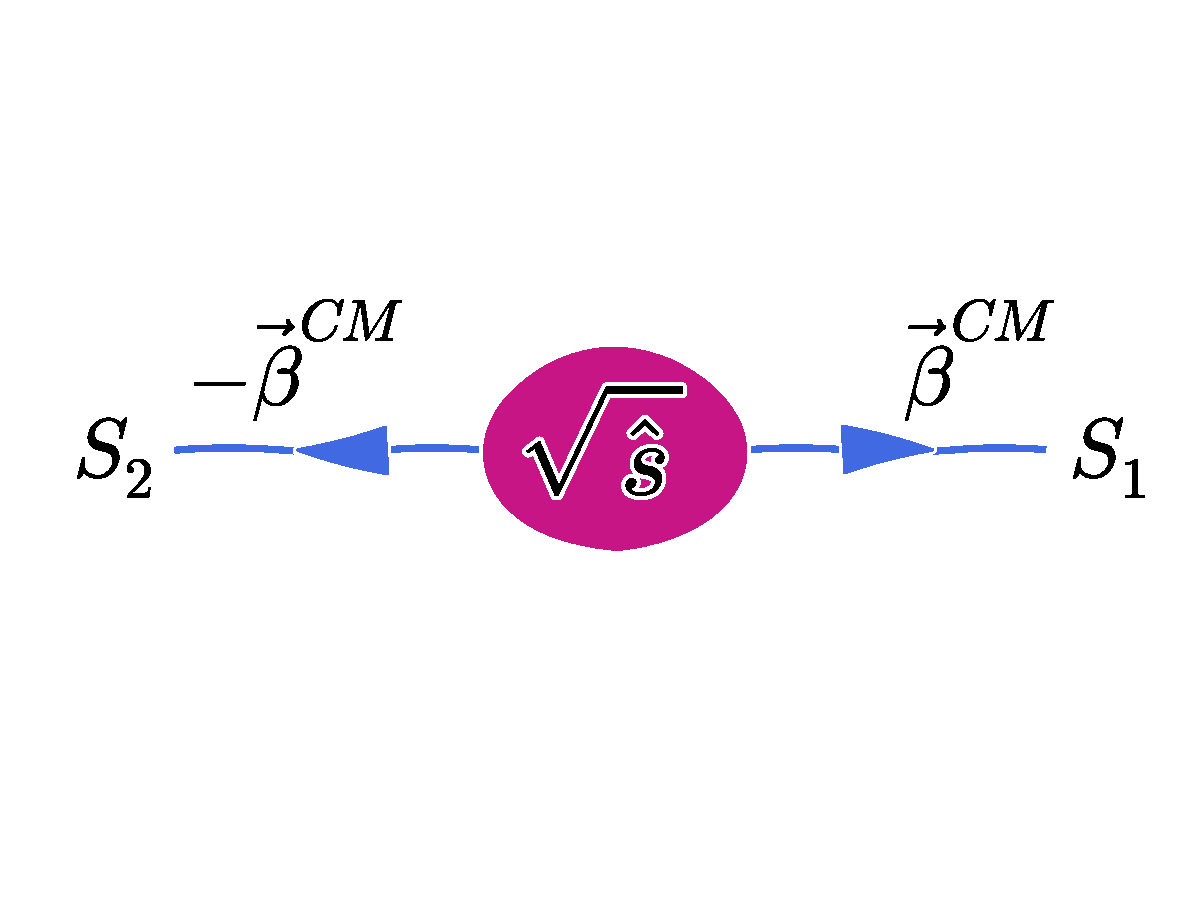
\includegraphics[width=0.6\textwidth,clip=true,trim=0 5.5cm 0
4.5cm]{figures/razor_variables/cm_frame} 
  \caption{Configuration of the center-of-mass frame. The particles $S_1$ and $S_2$ are
produced back to back with velocities $\betaCM$ and $-\betaCM$, respectively. 
\label{fig:razor_CM_frame}}
\end{figure}

To go from the rest frame of $S_1$ ($S_2$) to the CM frame, we need to boost the four-momenta
$q_1^S$ and $\nu_1^S$ ($q_2^S$ and $\nu_2^S$) to the frame travelling at velocity $\betaCM$
($-\betaCM$) with respect to the $S_1$ ($S_2$) rest frame. 
The four-vectors of particles $S_1$ and $S_2$ in the center-of-mass frame are also obtained by
boosting according to $\betaCM$. They can be written as
\begin{alignat}{6}
  P[S_1] &\equiv s^{\textrm{CM}}_1  &&= \{ E^{\textrm{CM}}_{S_1} , \vec{s}^{\textrm{CM}}_{S_1}\} 
&&= M_S \, \gamma^{\textrm{CM}} \, \{ 1 , \betaCM\} , \\ 
  P[S_2] &\equiv s^{\textrm{CM}}_2 &&= \{ E^{\textrm{CM}}_{S_2} , \vec{s}\,^{\textrm{CM}}_{S_2}\}
&&= M_S \, \gamma^{\textrm{CM}} \, \{ 1 , -\betaCM\},  
\end{alignat}
and satisfy the following
\begin{equation}
  (s^{\textrm{CM}}_1 + s^{\textrm{CM}}_1)^2 = \hat{s} = 4 (\gamma^{\textrm{CM}})^2 M_S^2,
\end{equation}
with $\sqrt{\hat{s}}$ the center-of-mass energy of the collision. 


\paragraph{Lab frame}
The lab frame is the frame where we make our measurements, and is related to the CM frame by a
boost $\vec{\beta}^{\textrm{lab}}$. We can decompose this boost into a transverse and longitudinal
part as $\vec{\beta}^{\textrm{lab}} = (\vec{\beta}_T,\vec{\beta}_z)$. 
The four-momenta of the $S_i$, $Q_i$ and $\chi_i$ particles are denoted by $s^{\textrm{lab}}_i$,
$q^{\textrm{lab}}_i$, and $\nu^{\textrm{lab}}_i$ respectively. 



\subsection{Derivation of \texorpdfstring{\mr}{MR} \label{sec:razor_mr}}

As mentioned in the previous section, our goal is to express the characteristic scale $M_\Delta$
using lab frame quantities only. Because the problem is kinematically underconstrained, we will
need to make some approximations as we work our way from the lab frame to the $S_i$ rest frame,
reversing the boosts $\vec{\beta}^{\textrm{lab}}$ and $\betaCM$ as we go along. 

The models of new physics that we aim to target with the razor variables all predict that the new
particles are heavy. This prediction is the basis of the two approximations we will be making. 

\begin{enumerate}
  \item If $M_S$ is large compared to $\sqrt{s}$, then the particles $S_1$ and $S_2$ will be
produced near the $\sqrt{\hat{s}} = 2 M_S$ threshold. This means that $\gamma^{\textrm{CM}} \approx
1$. We will thus assume that $\gamma^{\textrm{CM}} = 1$, which means that $\betaCM \rightarrow 0$. 
The CM frame is thus equal to both $S_i$ rest frames after this first approximation. 
  \item The transverse boost between lab frame and CM frame can be approximated by 
  \begin{equation}
    |\vec{\beta}_T| \approx \frac{p_T^{ISR}}{\sqrt{\hat{s}}} \lesssim \frac{p_T^{ISR}}{2M_S},
  \end{equation}
  where $p_T^{ISR}$ is the magnitude of the vectorial sum of the transverse momentum of the initial
state radiation. For large values of $M_S$ we find $\vec{\beta}_T \ll 1$. We thus assume that
$\vec{\beta}_T \rightarrow 0$, and thus $\vec{\beta}^{\textrm{lab}} \rightarrow \vec{\beta}_z$.
\end{enumerate}
The results of these two approximations is that we only need a longitudinal boost $\vec{\beta}_z$
to take us from the lab frame to the approximate $S_i$ rest frames. 
In this so-called \textit{rough-approximation frame}, or \textit{R-frame}, we have that
\begin{alignat}{4}
  |\vec{q}^R_1|         &= |\vec{q}^R_2| &&= \frac{M_\Delta}{2} , \\
  \textrm{or } E_{Q_1}^R &= E_{Q_2}^R     &&= \frac{M_\Delta}{2}.
\label{eq:razor_equal_energy_R_frame}
\end{alignat}
cf. Eq.~\ref{eq:razor_equal_momenta}. Using this constraint, we can compute the boost $\beta^R$
that will take us from the lab frame to the R-frame. We start from the basic Lorentz
transformations for energy and momentum, 
\begin{align}
  E_{Q_i}^R      &= \gamma^R \left( E_{Q_i}^{\textrm{lab}} - \beta^R \vec{q}_{iz}^{\textrm{lab}}
\right) , \\
  \vec{q}_{iz}^R &= \gamma^R \left( \vec{q}_{iz}^{\textrm{lab}} - \beta^R E_{Q_i}^{\textrm{lab}}
\right) .
\end{align}
Using Eq.~\ref{eq:razor_equal_energy_R_frame} we find
\begin{equation}
  E_{Q_1}^{\textrm{lab}} - \beta^R \vec{q}_{1z}^{\textrm{lab}} = E_{Q_2}^{\textrm{lab}} - \beta^R
\vec{q}_{2z}^{\textrm{lab}} ,
\end{equation}
and thus for the boost $\beta^R$
\begin{equation}
  \beta^R = \frac{E_{Q_1}^{\textrm{lab}} - E_{Q_2}^{\textrm{lab}}}{\vec{q}_{1z}^{\textrm{lab}} -
\vec{q}_{2z}^{\textrm{lab}}} . \label{eq:razor_beta_R}
\end{equation}
The Lorentz factor $\gamma^R$ can be expressed as
\begin{align}
  \gamma^R &= \frac{1}{\sqrt{1 - (\beta^R)^2}} \\
	   &= \frac{1}{\sqrt{1 - \left( \frac{E_{Q_1}^{\textrm{lab}} -
E_{Q_2}^{\textrm{lab}}}{\vec{q}_{1z}^{\textrm{lab}} -
\vec{q}_{2z}^{\textrm{lab}}} \right)^2}} \\
           &= \frac{ \vec{q}_{1z}^{\textrm{lab}} - \vec{q}_{2z}^{\textrm{lab}} }{\sqrt{ \left(
 \vec{q}_{1z}^{\textrm{lab}} - \vec{q}_{2z}^{\textrm{lab}} \right)^2 - \left(
 E_{Q_1}^{\textrm{lab}} - E_{Q_2}^{\textrm{lab}}\right)^2 }} \label{eq:razor_gamma_R}
\end{align}

We now define \mr as
\begin{equation}
  \mr \equiv 2 |\vec{q}^R| = M_\Delta .
\end{equation}
It is interesting to note that \mr is invariant under longitudinal boosts. Using
Eq.~\ref{eq:razor_beta_R} and Eq.~\ref{eq:razor_gamma_R}, we can express \mr using lab frame
quantities only. 

\begin{align}
  \mr &= E_{Q_1}^R + E_{Q_2}^R \\
      &= \gamma^R \left( E_{Q_1}^{\textrm{lab}} + E_{Q_2}^{\textrm{lab}} - \beta^R (
\vec{q}_{1z}^{\textrm{lab}} + \vec{q}_{2z}^{\textrm{lab}}) \right) \\
      &= \frac{\left( \vec{q}_{1z}^{\textrm{lab}} - \vec{q}_{2z}^{\textrm{lab}}\right) 
               \left( E_{Q_1}^{\textrm{lab}} + E_{Q_2}^{\textrm{lab}} - \frac{E_{Q_1}^{\textrm{lab}}
- E_{Q_2}^{\textrm{lab}}}{\vec{q}_{1z}^{\textrm{lab}} - \vec{q}_{2z}^{\textrm{lab}}}
(\vec{q}_{1z}^{\textrm{lab}} + \vec{q}_{2z}^{\textrm{lab}}) \right)}
              { \sqrt{ \left( \vec{q}_{1z}^{\textrm{lab}} - \vec{q}_{2z}^{\textrm{lab}} \right)^2 
                      -\left( E_{Q_1}^{\textrm{lab}} - E_{Q_2}^{\textrm{lab}}\right)^2 }} \\
      &= \frac{\left( \vec{q}_{1z}^{\textrm{lab}} - \vec{q}_{2z}^{\textrm{lab}} \right) 
               \left( E_{Q_1}^{\textrm{lab}} + E_{Q_2}^{\textrm{lab}} \right) 
               - 
               \left( E_{Q_1}^{\textrm{lab}} - E_{Q_2}^{\textrm{lab}} \right)
               \left( \vec{q}_{1z}^{\textrm{lab}} + \vec{q}_{2z}^{\textrm{lab}} \right) }
              { \sqrt{ \left( \vec{q}_{1z}^{\textrm{lab}} - \vec{q}_{2z}^{\textrm{lab}} \right)^2 
                      -\left( E_{Q_1}^{\textrm{lab}} - E_{Q_2}^{\textrm{lab}}\right)^2 }} \\
      &= \frac{2 \left( \vec{q}_{1z}^{\textrm{lab}} E_{Q_2}^{\textrm{lab}} 
                       - \vec{q}_{2z}^{\textrm{lab}} E_{Q_1}^{\textrm{lab}} \right)}
              { \sqrt{ \left( \vec{q}_{1z}^{\textrm{lab}} - \vec{q}_{2z}^{\textrm{lab}} \right)^2 
                      -\left( E_{Q_1}^{\textrm{lab}} - E_{Q_2}^{\textrm{lab}}\right)^2 }}
\end{align}
Our final expression for \mr in lab frame quantities becomes
\begin{equation}
  \mr = 2 \sqrt { \frac{ \left( \vec{q}_{1z}^{\textrm{lab}} E_{Q_2}^{\textrm{lab}} 
                       - \vec{q}_{2z}^{\textrm{lab}} E_{Q_1}^{\textrm{lab}} \right) ^2}
                       { \left( \vec{q}_{1z}^{\textrm{lab}} - \vec{q}_{2z}^{\textrm{lab}}
\right)^2 
                        -\left( E_{Q_1}^{\textrm{lab}} - E_{Q_2}^{\textrm{lab}}\right)^2 }} . 
\end{equation}
As the R-frame is only an approximation of the $S_i$ rest frames, \mr will be distributed around
the characteristic scale $M_\Delta$ with degrading resolution as the Lorentz factor increases. 
More generally, the peak value of \mr scales as $\gamma^{\textrm{CM}}M_\Delta$.

We can use \mr as a way to distinguish signal from background, in particular background from QCD
multijet production. Let's consider QCD dijet production. In the dijet rest frame we have for the
four-momenta of the two jets, $k_1$ and $k_2$
\begin{align}
  k_1 &= \frac{\sqrt{\hat{s}}}{2} \{1, \vec{v}\} ,\\
  k_2 &= \frac{\sqrt{\hat{s}}}{2} \{1, -\vec{v}\},
\end{align}
where $\sqrt{\hat{s}}$ is the center-of-mass energy of the partonic subprocess, and $\vec{v}$ is a
unit vector along the dijet axis. For this type of event, $\mr = \sqrt{\hat{s}}$, and is thus
sharply falling. Signal will thus appear as a peak over a falling background. Given the large cross
sections for background processes, and small expected cross sections for signal processes, this
discrimination by itself is not sufficient. There is, however, more information available in the
event. We have yet to use the transverse degrees of freedom. These will be incorporated in \rsq, as
explained in the next section. 

\subsection{Derivation of \texorpdfstring{\rsq}{R2} \label{sec:razor_r2}}

We will now create a second way to estimate $M_\Delta$, utilizing the transverse information in the
event, as encoded in the missing transverse momentum. We start by defining the variable $M_{2S}$
using the four-vectors $q_i^{\textrm{lab}}$ and $\nu_i^{\textrm{lab}}$
\begin{equation}
  M_{2S} = \sqrt{\frac{1}{2} \left[  (q_1^{\textrm{lab}} + \nu_1^{\textrm{lab}})^2 +
(q_2^{\textrm{lab}} + \nu_2^{\textrm{lab}})^2 \right] } . \label{eq:razor_M2S}
\end{equation}
As the sum $q_i^{\textrm{lab}} + \nu_i^{\textrm{lab}}$ is just the four-vector associated with
$S_i$, we immediately see that $M_{2S} = M_S$. Expanding Eq.~\ref{eq:razor_M2S} and using $M_{Q_i}
= 0$, we find
\begin{align}
  M_{2S} &= \sqrt{\frac{1}{2} \left( (q_1^{\textrm{lab}})^2 + 2 q_1^{\textrm{lab}}
\nu_1^{\textrm{lab}} + (\nu_1^{\textrm{lab}})^2 + (q_2^{\textrm{lab}})^2 + 2 q_2^{\textrm{lab}}
\nu_2^{\textrm{lab}} + (\nu_2^{\textrm{lab}})^2\right) } \\
         &= \sqrt{ q_1^{\textrm{lab}}\nu_1^{\textrm{lab}} + q_2^{\textrm{lab}}\nu_2^{\textrm{lab}}
+ M_\chi^2} \\
         &= \sqrt{ E^{\textrm{lab}}_{Q_1} E^{\textrm{lab}}_{\nu_1} - \vec{q}^{\textrm{lab}}_{1T}
\cdot \vec{\nu}^{\textrm{lab}}_{1T} - \vec{q}^{\textrm{lab}}_{1z} \cdot
\vec{\nu}^{\textrm{lab}}_{1z}
                  + E^{\textrm{lab}}_{Q_2} E^{\textrm{lab}}_{\nu_2} - \vec{q}^{\textrm{lab}}_{2T}
\cdot \vec{\nu}^{\textrm{lab}}_{2T} - \vec{q}^{\textrm{lab}}_{2z} \cdot
\vec{\nu}^{\textrm{lab}}_{2z} + M_\chi^2} .
\end{align}
Unfortunately we do not a priori know the mass of the $\chi_i$ particles. We will choose $M_\chi =
0$. As a result $M_{2S}$ will now give us a distribution, with endpoint at $M_S$. For the
particular case $M_\chi = 0$, we actually have $M_S = \frac{M_S^2-M_\chi^2}{M_S} = M_\Delta$.
Consequently, the endpoint of $M_{2S}$ gives us a second way to access the characteristic scale
$M_\Delta$.

The $\chi_i$ particles are assumed to be only weakly interacting. They pass through the detector
unseen. When we make the balance of momentum for each event, we can thus infer the existence of
these particles. At a hadron collider we can only make this balance in the transverse plane. The
transverse component of $M_{2S}$ is given by
\begin{equation}
  (M_{2S})_T = \sqrt{ |\vec{q}^{\textrm{lab}}_{1T}| |\vec{\nu}^{\textrm{lab}}_{1T}| -
\vec{q}^{\textrm{lab}}_{1T} \cdot \vec{\nu}^{\textrm{lab}}_{1T} 
                  + |\vec{q}^{\textrm{lab}}_{2T}| |\vec{\nu}^{\textrm{lab}}_{2T}| -
\vec{q}^{\textrm{lab}}_{2T} \cdot \vec{\nu}^{\textrm{lab}}_{2T}} ,
\end{equation}
where we have used the assumptions that both $Q_i$ and $\chi_i$ are massless. 
In the considered signal topology we have two unseen particles, $\chi_1$ and $\chi_2$.
Experimentally we can only access the sum of their transverse momenta, which in absence of detector
effects is given by the missing transverse momentum \VEtmiss. Making the assumption that the
\VEtmiss is divided equally among both $\chi_i$ particles, we find
\begin{equation}
  \mtr = \sqrt{\frac{|\VEtmiss|}{2} \left(|\vec{q}^{\textrm{lab}}_{1T}| +
|\vec{q}^{\textrm{lab}}_{2T}| \right) - \frac{\VEtmiss}{2} \cdot \left(\vec{q}^{\textrm{lab}}_{1T} +
\vec{q}^{\textrm{lab}}_{2T} \right)} .
\end{equation}

We now define the dimensionless variable $\mathrm{R}$ as
\begin{equation}
  \mathrm{R} \equiv \frac{\mtr}{\mr} .
\end{equation}
This variable peaks at around 0.5 for signal events, since it is the ratio of two variables that
estimate the same scale, with an additional geometric factor to take into account that
$\mathrm{M_T^R}$ only contains transverse information. For QCD dijet events $\mathrm{R}$ equals 0
for an ideal detector. Placing a minimum requirement on this variable can thus
be effectively used to suppress background events.


\subsection{Improved \texorpdfstring{\mr and \rsq}{MR and R2} definitions
\label{sec:razor_mr_r2_improved}}

The razor frame as defined in the previous section has a number of useful features, such as \mr
being invariant under longitudinal boosts. It also has one important issue which can occur if the
approximation $\gamma^{\textrm{CM}} = 1$ breaks down. The issue is visible from the expression of
$\beta^R$ in Eq.~\ref{eq:razor_beta_R}. Looking at that equation, we see that it is possible to get
a situation where $|\beta^R| \geq 1$. The boost is then unphysical, and the razor frame ill-defined.
We can remedy this issue by not neglecting $\vec{\beta}_T$, the transverse component of
$\betaCM$. 

% TODO Add the full computation

We again start by making a longitudinal boost $\beta^{L*}$ from the lab frame. Then we apply a
transverse boost $\vec{\beta}_T^{\mathrm{R}*}$. This boost is applied in opposite directions to the
decay products of $S_1$ and $S_2$. The two resulting frames are called $\mathrm{R}*$-frames, and
have to satisfy the requirement that the magnitude of the momenta of $Q_1$ and $Q_2$ in their
respective $\mathrm{R*}$-frame are equal. 

This constraint can be rewritten as
\begin{equation}
  \gamma^{L*} (E_{Q_1}^{\textrm{lab}} - E_{Q_2}^{\textrm{lab}}) - \gamma^{L*} \beta^{L*}
(q_{1z}^{\textrm{lab}} - q_{2z}^{\textrm{lab}}) = \vec{\beta}_T^{R*} \cdot
(\vec{q}_{1T}^{\textrm{lab}} + \vec{q}_{2T}^{\textrm{lab}}), 
\end{equation}
where we have used the Lorentz transformations for energy corresponding to the two consecutive
boosts,
\begin{align}
  E_{Q_i}^{L*} &= \gamma^{L*} (E_{Q_i}^{\textrm{lab}} - \beta^{L*} q_{iz}^{\textrm{lab}} ) , \\
  E_{Q_1}^{R*} &= \gamma_T^{R*} (E_{Q_1}^{L*} - \vec{\beta}_T^{R*} \cdot
\vec{q}_{1T}^{\textrm{lab}}) , \\
  E_{Q_2}^{R*} &= \gamma_T^{R*} (E_{Q_2}^{L*} + \vec{\beta}_T^{R*} \cdot
\vec{q}_{2T}^{\textrm{lab}}) .
\end{align}
Introducing the unit vector $\hat{\beta}_T^{\mathrm{R}*}$ such that $\vec{\beta}_T^{\mathrm{R}*} =
\beta_T^{\mathrm{R}*} \hat{\beta}_T^{\mathrm{R}*}$, we find for the magnitude of the transverse
boost
\begin{equation}
  \beta_T^{\mathrm{R}*} = \frac{\gamma^{L*} (E_{Q_1}^{\textrm{lab}} - E_{Q_2}^{\textrm{lab}}) -
\gamma^{L*} \beta^{L*} (q_{1z}^{\textrm{lab}} - q_{2z}^{\textrm{lab}})}{\hat{\beta}_T^{R*} \cdot
(\vec{q}_{1T}^{\textrm{lab}} + \vec{q}_{2T}^{\textrm{lab}})}
\end{equation}

In analogy with our previous discussion we define the $\mathrm{R}*$-frame mass $\mathrm{M_{R*}}$ as
\begin{align}
  \mathrm{M_{R*}} &\equiv 2 |\vec{q}_1^{\mathrm{R}*}| = 2 |\vec{q}_2^{\mathrm{R}*}| \\
                  &= \frac{2\gamma^{L*} \hat{\beta}_T^{\mathrm{R}*} \cdot \left[
(E_{Q_1}^{\textrm{lab}}\vec{q}_{2T}^{\textrm{lab}} +
E_{Q_2}^{\textrm{lab}}\vec{q}_{1T}^{\textrm{lab}}) - \beta^{L*}
(q_{1z}^{\textrm{lab}}\vec{q}_{2T}^{\textrm{lab}} +
q_{2z}^{\textrm{lab}}\vec{q}_{1T}^{\textrm{lab}}) \right]}
                           {\sqrt{|\hat{\beta}_T^{R*} \cdot (\vec{q}_{1T}^{\textrm{lab}} +
\vec{q}_{2T}^{\textrm{lab}})|^2 - (\gamma^{L*})^2 \left[ E_{Q_1}^{\textrm{lab}} -
E_{Q_2}^{\textrm{lab}} - \beta^{L*} (q_{1z}^{\textrm{lab}} - q_{2z}^{\textrm{lab}}) \right]^2}}
\end{align}

To fully compute $\mathrm{M_{R*}}$ we need to pick a value for $\beta_T^{\mathrm{R}*}$ and
$\beta^{L*}$. The configurations that led to unphysical \mr values have the property that the
momenta of $Q_1$ and $Q_2$ point in the same direction in the transverse plane, with $\betaCM$
pointing in the same or the opposite direction. Based on this observation, we choose a direction
for $\hat{\beta}_T^{\mathrm{R}*}$ that maximizes $|\hat{\beta}_T^{R*} \cdot
(\vec{q}_{1T}^{\textrm{lab}} + \vec{q}_{2T}^{\textrm{lab}})|$. The direction that maximizes this
quantity is aligned with the direction of $\vec{q}_{1T}^{\textrm{lab}} +
\vec{q}_{2T}^{\textrm{lab}}$. Realizing that a unit vector can be expressed as a vector indicating
the direction divided by the norm of that vector, we find for $\hat{\beta}_T^{\mathrm{R}*}$ 
\begin{equation}
  \hat{\beta}_T^{\mathrm{R}*} = \frac{\vec{q}_{1T}^{\textrm{lab}} +
\vec{q}_{2T}^{\textrm{lab}}}{|\vec{q}_{1T}^{\textrm{lab}} + \vec{q}_{2T}^{\textrm{lab}}|}
\label{eq:razor_beta_T_Rstar}
\end{equation}
We still want $\mathrm{M_{R*}}$ to be invariant under longitudinal boosts. Therefore we choose
$\beta^{L*}$ according to the condition $\frac{\partial \mathrm{M_{R*}}}{\partial \beta^{L*}} = 0$.
We find
\begin{equation}
  \beta^{L*} = \frac{q_{1z}^{\textrm{lab}} + q_{2z}^{\textrm{lab}}}
{E_{Q_1}^{\textrm{lab}} + E_{Q_2}^{\textrm{lab}}}
\label{eq:razor_beta_Lstar}
\end{equation}

Substituting Eq.~\ref{eq:razor_beta_T_Rstar} and Eq.~\ref{eq:razor_beta_Lstar} in the expression for
$\mathrm{M_{R*}}$ we find
\begin{equation}
  \mathrm{M_{R*}} = \sqrt{\left( E_{Q_1}^{\textrm{lab}} + E_{Q_2}^{\textrm{lab}}\right)^2 
                        - \left( q_{1z}^{\textrm{lab}} + q_{2z}^{\textrm{lab}} \right)^2 
                        - \frac{(|\vec{q}_{1T}^{\textrm{lab}}|^2 -
|\vec{q}_{2T}^{\textrm{lab}}|^2 )^2}{|\vec{q}_{1T}^{\textrm{lab}} +
\vec{q}_{2T}^{\textrm{lab}}|^2} } .
\end{equation}
We can also express $\gamma_T^{R*}$ in lab frame observables,
\begin{equation}
  \gamma_T^{R*} = \sqrt{ \frac{\left( E_{Q_1}^{\textrm{lab}} + E_{Q_2}^{\textrm{lab}}\right)^2 
                        - \left( q_{1z}^{\textrm{lab}} + q_{2z}^{\textrm{lab}} \right)^2 }
                              {\left( E_{Q_1}^{\textrm{lab}} + E_{Q_2}^{\textrm{lab}}\right)^2 
                        - \left( q_{1z}^{\textrm{lab}} + q_{2z}^{\textrm{lab}} \right)^2 
                        - \frac{(|\vec{q}_{1T}^{\textrm{lab}}|^2 -
|\vec{q}_{2T}^{\textrm{lab}}|^2 )^2}{|\vec{q}_{1T}^{\textrm{lab}} +
\vec{q}_{2T}^{\textrm{lab}}|^2}}} . 
\end{equation}
The peak value of the $\mathrm{M_{R*}}$ distribution is at $M_\Delta$, whereas the peak value for
$\gamma_T^{R*}\mathrm{M_{R*}}$ is at $\gamma^{\textrm{CM}}M_\Delta$, as was the case for \mr
earlier. This motivates us to redefine \mr as
\begin{equation}
  \mr = \gamma_T^{R*}\mathrm{M_{R*}} = \sqrt{\left( E_{Q_1}^{\textrm{lab}} +
E_{Q_2}^{\textrm{lab}}\right)^2 - \left( q_{1z}^{\textrm{lab}} +
q_{2z}^{\textrm{lab}} \right)^2} ,
\end{equation}
which is still longitudinally invariant, but does not suffer from unphysical boosts.
The definition of \mtr remains the same, and $\mathrm{R} = \frac{\mtr}{\mr}$ is now defined using
the updated \mr definition.

\subsection{Generalization to longer decay chains \label{sec:razor_megajet_algorithm}}

In the previous discussion we have always assumed that the new particles decay according to a
two-body decay chain. We can of course envision many other scenarios in which this is no longer the
case. One could have three- or four-body decays, or long decay chains. All of those cases would
result in more than two visible particles in the final state. 

In order to use the same razor formalism, we simply need to cluster all the particles in the event
into two so-called \textit{megajets}. Among all possible clusterings of particles in two groups, we
choose the clustering that minimizes the quadratic sum of invariant masses of the two megajets. The
four-momenta of the megajets, which are used to compute the invariant masses, are defined as the sum
of the four-momenta of their constituents. \mr and \rsq are then defined as before, using the
megajets as the two visible components. 

This approach groups particles travelling in the same direction, and is effective at grouping the
decay products of each of the two initially produced particles. 


\subsection{The razor variables in the razor boost analysis}

As the name already indicates, the razor boost analysis uses the razor variables as the main
discriminating variables. They are well suited for the purpose of the analysis, as they are
designed to describe a signal due to pair production of heavy particles, each of which decays to a
massless visible particle and a massive invisible particle, as is the case for the targeted models
in the razor boost analysis. The signal will appear as a peak on an exponentially falling
background. 

For clarity we repeat the \mr and \rsq definitions here, replacing the relevant variables with their
megajet counterparts (indices $j_i$), 
\begin{align}
  \mr &= \sqrt{\left( E_{j_1} + E_{j_2}\right)^2 - \left( p_{z}^{j_1} + p_{z}^{j_2} \right)^2} ,\\
  \rsq &= \frac{\mtr}{\mr} ,\\
  \textrm{with } \mtr &= \sqrt{\frac{|\VEtmiss|}{2} \left(p^{j_1}_{T} + p^{j_2}_{T}
\right) - \frac{\VEtmiss}{2} \cdot \left(\vec{p}^{j_1}_{T} + \vec{p}^{j_2}_{T} \right)} ,
\end{align}
where we have defined $p_T$ as the magnitude of the transverse momentum vector $\vec{p}_T$. 

The two-dimensional (2D) distributions of \rsq versus \mr for both background and an example signal
model are shown in Fig.~\ref{fig:razor_MR_Rsq_bg_signal}. It is clear that the background,
dominated by QCD multijet production, is located in the low \mr and low \rsq regions, and falls of
steeply when \mr or \rsq is increased. The signal, on the other hand, shows a peaking behaviour in
\mr and is located substantially higher in the (\mr,\rsq) space. 

\begin{figure}[htpb]
\centering
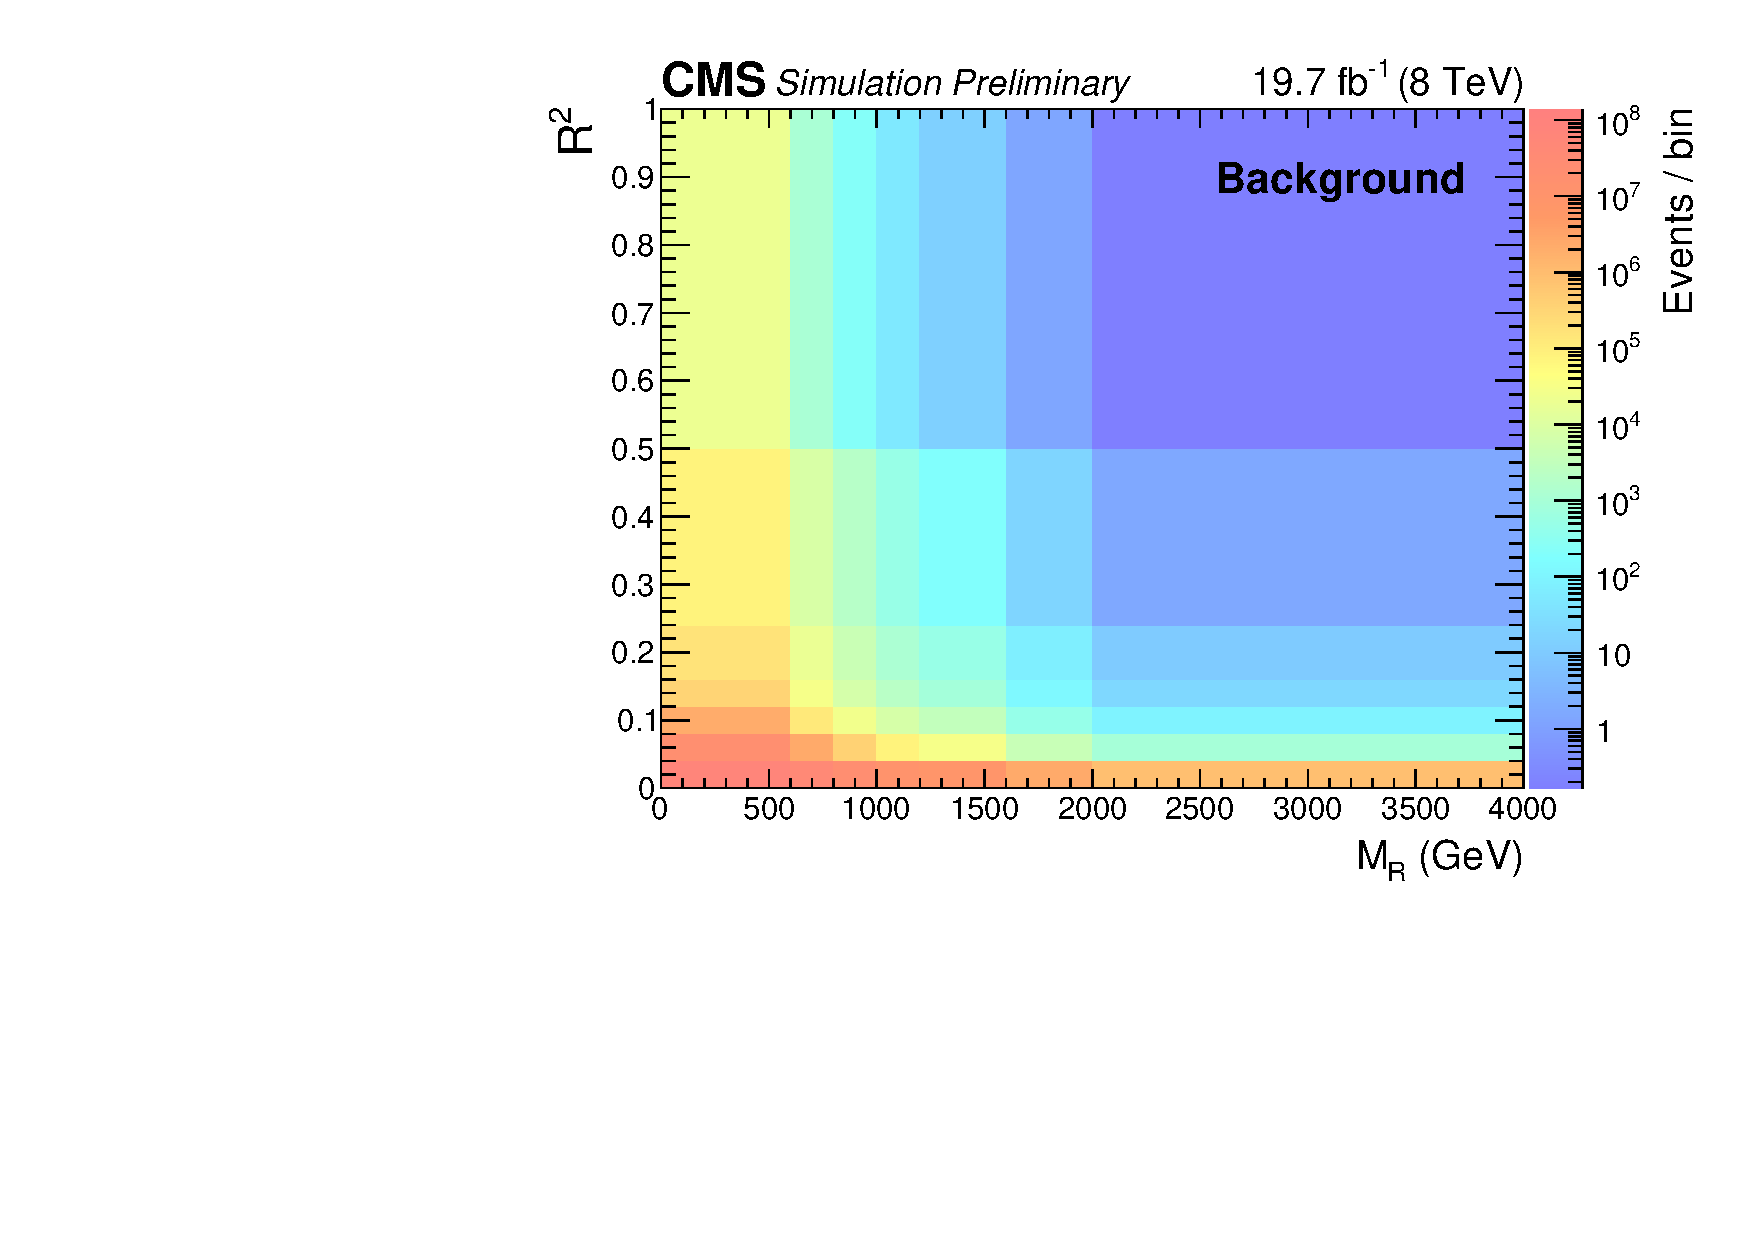
\includegraphics[width=0.49\textwidth]{figures/razor_variables/MR_R2_jet1ptg200_bg} 
\includegraphics[width=0.49\textwidth]{figures/razor_variables/MR_R2_jet1ptg200_sig}
\caption{Distribution of the overall SM backgrounds and a T1ttcc signal with $m_{\tilde{g}} \,{=}\,
1\TeV$, $m_{\tilde{t}} \,{=}\, 325\GeV$ and $m_{\tilde{\chi}_1^0} \,{=}\, 300\GeV$, both obtained
from MC, on the (\mr,\rsq) space. A very loose selection is used:  a good primary vertex and at
least three jets, one of which should have $\pt > 200$ \GeV. 
\label{fig:razor_MR_Rsq_bg_signal}}

\end{figure}




\section[Boosted W boson tagging]{Boosted $\W$ boson tagging \label{sec:boost_wtag}}

%%%%%%%%%%%%%%%%%
% W tagging
%%%%%%%%%%%%%%%%%

One of the main highlights of the razor boost analysis is the tagging of boosted $\W$ bosons in
order to access a signal dominated phase space. 
$\W$ bosons either decay to two quarks, or to a lepton and a neutrino. The razor boost analysis is
an all-hadronic analysis, which means we do not explicitly consider the leptonic decays. 
$\W$ bosons with low to moderate transverse momentum will thus result in two jets, corresponding to
the two clusters of particles resulting from the hadronization of the two quarks. 
As the $\pt$ of the $\W$ boson increases, the separation between the two resulting jets decreases.
For high enough momentum, the two jets can no longer be fully resolved with the usual jet
definitions, and will be reconstructed as a single jet. This turnover in efficiency between the
resolved and merged case is illustrated in Fig.~\ref{fig:boost_wtag_ca8eff}.
Depending on the requirements on the jet multiplicity, losing a jet can result in a loss of signal
efficiency. We can, however, also use this effect to our advantage, namely to increase the
signal-to-background ratio by requiring the presence of one of these \textit{merged} jets. 
This, in turn, allows us to relax the jet multiplicity requirements. 

\begin{figure}
  \centering
  \includegraphics[width=0.8\textwidth]{figures/razor_wtag/ca8effVsPt}
  \caption{Efficiency to reconstruct a CA8 jet within $\Delta R<0.1$ of a generated $\W$ boson, and
the efficiency to reconstruct two AK5 jets within $\Delta R<0.1$ of the generated quarks from
longitudinally polarized $\W$ bosons, as a function of the $\pt$ of the $\W$
boson~\cite{Khachatryan:2014vla}. The loss in efficiency for the resolved case is clearly visible
for high $\pt$ $\W$ bosons. 
  \label{fig:boost_wtag_ca8eff}}
\end{figure}

The merged jet can be distinguished from other jets by its jet substructure, as illustrated in
Fig.~\ref{fig:boost_wtag_cartoon}. Jets originating from a $\W$ boson should have a two-prong
structure, whereas a quark/gluon-initiated jet is not expected to have this structure. 
In recent years, jet substructure techniques have seen very active developments, and many different
algorithms are on the market~\cite{Krohn:2009th,Gallicchio:2010sw,Butterworth:2008iy,Kaplan:2008ie}.
For the razor boost analysis we will use the CMS recommendation
in terms of which techniques to use~\cite{CMS-PAS-JME-13-006,Khachatryan:2014vla}. We will employ
\textit{jet pruning} and a set of variables called \textit{N-subjettiness}. On top of these jet
substructure techniques we will also use the jet mass variable to distinguish $\W$ boson-initiated
jets
from quark/gluon-initiated jets. 
The following subsections will go through the different parts of the
$\W$ tagging definition, providing a more detailed explanation for each.

\begin{figure}
  \centering
  \includegraphics[width=0.48\textwidth]{figures/razor_wtag/W_subjets}
  ~
  \includegraphics[width=0.48\textwidth]{figures/razor_wtag/qg_jets}
  \caption{The jet substructure of a $\W$-initiated jet differs from a quark/gluon-initiated jet.
  \label{fig:boost_wtag_cartoon}}
\end{figure}

%%%%%%%%%%%%%%%%%%%%%%%%%%%%%%%%%%%%%%%%%%%%%%%%%%%%%%%%%%%%%%%%%%%%%%%%%%%%%%%%%%%%%%%%%%%%%%%%%%%%

\subsection{Jet algorithm}

In order to identify boosted $\W$ bosons,  we will use a different jet clustering algorithm
than what is used for the standard jet definition (see Section~\ref{sec:object_jets}). 
Jets will be clustered with \textsc{FastJet 3.0.1.}~\cite{Cacciari:2011ma}, from the PF candidates,
using the Cambridge-Aachen (CA) algorithm~\cite{Dokshitzer:1997in} with a size parameter of 0.8.
Henceforth, we will call these jets \textit{CA8 jets}. 

%\begin{quote}
\begin{cajet} \theoremstyle{definition}
The Cambridge-Aachen jet algorithm is a sequential recombination algorithm that uses the
distance measure $d_{ij}$ between two constituents $i$ and $j$,
\begin{equation}
d_{ij} = \frac{\Delta R_{ij}^2}{R^2}, \label{eq:CA_distance}
\end{equation}
with $R$ the size parameter of the resulting jets, and
\begin{equation}
\Delta R_{ij}^2 = (y_i - y_j)^2 + (\phi_i - \phi_j)^2 ,
\label{eq:DeltaR_jet_algo}
\end{equation}
where $y, \phi$ are the rapidity (defined in Eq.~\ref{eq:rapidity}) and azimuthal angle. 
%The rapidity is given in terms of energy and longitudinal momentum as
%\begin{equation}
%  y = \frac{1}{2} \ln{\frac{ E + p_z }{ E - p_z }} .
%\end{equation}
The distance between constituent $i$ and the beam is given by $d_{iB} = 1$.
As is clear from the above, these distance measures only use angular information, unlike for the
$k_\mathrm{T}$ and anti-$k_\mathrm{T}$ algorithms, which use a $\pt$-weighted distance. 

The jet algorithm starts by computing the minimum distance $d_{ij}$, across all $i,j$. If $\min
d_{ij} < d_{iB}$, then we combine constituents $i$ and $j$ into a new constituent whose
four-momentum is the sum of the four-momenta of $i$ and $j$, and repeat the process. Otherwise, we
call $i$ a jet and move it from the list of constituents to be clustered to the list of final jets.
The process is repeated with the remaining constituents, until none remain.
\end{cajet}


Jet energy corrections for these CA8 jets are derived from the standard anti-$k_\textrm{T}$ jets
with size parameter $R=0.7$. Simulations show that the corrections are valid for CA8 jets and
have an additional uncertainty no greater than 2\%~\cite{CMS-PAS-JME-13-007,CMS-AN2012-393}.  
% seems like no better reference is available for this...

%%%%%%%%%%%%%%%%%%%%%%%%%%%%%%%%%%%%%%%%%%%%%%%%%%%%%%%%%%%%%%%%%%%%%%%%%%%%%%%%%%%%%%%%%%%%%%%%%%%%

\subsection{Jet pruning}

Jet pruning~\cite{Ellis:2009su,Ellis:2009me} is a particular kind of jet grooming. Jet grooming
techniques are designed to reduce the impact of contributions from the underlying event (UE), pileup
(PU), and low-\pt gluon radiation. These kinds of contributions to jets are typically soft and
diffuse, and increase the jet energy proportional to the jet area. Grooming techniques reduce the
jet area without affecting the core components. This means that the resulting jets are less
sensitive to these soft contributions, but still reflect the kinematics of the original, hard
process.


During jet pruning the constituents of the jet are reclustered with the CA algorithm, using the
same distance parameter as used for the original jets (here $R=0.8$), but with additional conditions
beyond those of the standard algorithm.
In particular, the softer and larger-angle of the two particles $i$ and $j$ to be merged is removed
when the following conditions are satisfied:
\begin{align}
  z_{ij} &= \frac{\min( \pt^i , \pt^j )}{\pt^i + \pt^j} < z_{\textrm{cut}}, \\
  \Delta R_{ij} &> D_{\textrm{cut}} \equiv \alpha \frac{m_J}{\pt} ,
\end{align}
where $m_J$ and $\pt$ are the original mass and transverse momentum of the reclustered jet,
$\Delta R_{ij}$ is defined as in Eq.~\ref{eq:DeltaR_jet_algo}, and
$z_\textrm{cut}$ and $\alpha$ are parameters of the algorithm, chosen to be 0.1 and 0.5,
respectively~\cite{Chatrchyan:2013vbb}. 

The resulting pruned jet is used as further input to our $\W$ boson tagger. For the $\W$ decay
products to be collimated, we need a large transverse momentum. We will therefore require that the
pruned jets have $\pt > 200\GeV$. 
Because of the reduction of the effect of UE and PU, the jet mass variable as computed from the
constituents of the jet after jet pruning has a much better behaviour than if it was computed from
the unpruned jets, as seen on Fig.~\ref{fig:wtag_jet_pruning}. Jet pruning shifts the jet mass of
QCD jets
to smaller values, while maintaining the jet mass for $\W$ jets close to the $\W$ boson mass.

We will make the requirement that the pruned jet mass is consistent with the $\W$ boson mass,
\begin{equation}
  70 < m_{\textrm{pruned jet}} < 100 \GeV .
\end{equation}
Here, we have deviated from the standard interval used in CMS, starting at 60\GeV, as we found that
for our
kinematical region and signal topology we achieve better signal to background discrimination when
increasing the lower cut value to 70\GeV. 
%This provides good boosted $\W$ jet to quark/gluon jet discrimination. 

\begin{figure}
  \centering
  \includegraphics[width=0.6\textwidth]{figures/razor_wtag/1DPFCHS_PR_QCD}
  \caption{Jet mass distribution of QCD jets with $\pt(\textrm{gen}) > 300 \GeV$ for jet pruning
with different parameters, starting from PF jets with charged-hadron subtraction applied. The fully
ungroomed mass distribution is also shown for comparison. Here, the jets were clustered using the
anti-$k_\mathrm{T}$ algorithm, but the same picture holds for Cambridge-Aachen jets.
Figure taken from~Ref.\cite{CMS-PAS-JME-14-001}. 
  \label{fig:wtag_jet_pruning}}
\end{figure}

%%%%%%%%%%%%%%%%%%%%%%%%%%%%%%%%%%%%%%%%%%%%%%%%%%%%%%%%%%%%%%%%%%%%%%%%%%%%%%%%%%%%%%%%%%%%%%%%%%%%

\subsection{N-subjettiness}

Requiring the jet mass to be consistent with the $\W$ boson mass already results in a good
discrimination between $\W$ boson and quark/gluon-initiated jets. We can, however, still do better.
A boosted QCD jet with a mass around 80\GeV usually originates from a single hard parton and
acquires mass through large-angle soft splittings. The energy pattern for this process will differ
from the two-prong pattern that is found in boosted $\W$ jets.  
The set of N-subjettiness observables $\tau_N$~\cite{Thaler:2010tr} aims to exploit this difference
in expected energy flow to differentiate between $\W$ boson and quark/gluon-initiated jets by
counting the number of hard lobes of energy within a jet.

N-subjettiness is computed under the assumption that the jet has N subjets, and is the
$\pt$-weighted $\Delta R$ distance between each jet constituent and its nearest subjet axis:
\begin{equation}
\tau_N = \frac{1}{R_0 \sum_{k} p_{T, k}} \sum_k p_{T, k} \min (\Delta R_{1,k}, \Delta R_{2,k}, ...
\Delta R_{N,k}),
\end{equation}
where $R_0$ is the original jet distance parameter (0.8 in our case) and $k$ runs over all
constituent particles of the jet. 
The subjet axes are obtained by running the exclusive $k_T$
algorithm~\cite{Ellis:1993tq,Catani:1993hr} using \textsc{FastJet}. 
The exclusive $k_T$ algorithm differs from the inclusive version in two ways: if at a given
clustering step $d_{iB} < \min_j d_{ij}$, then constituent $i$ is discarded, rather than added to
the jet collection; and the clustering stops when the desired number of jets (N) is reached. 
The resulting axes can be further optimized to minimize the N-subjettiness value. In accordance to
the CMS recommendation, we use a “one-pass” optimization of the exclusive $k_T$
axes~\cite{nsubjettiness_fastjet}.

The variables $\tau_N$ quantify the consistency of the jet having N or fewer subjets. They have a
small value (close to 0) if the original jet is consistent with having N or fewer subjets, because
almost every jet constituent will be close in $\Delta R$ to its own true subjet. 
As we are interested in discriminating boosted $\W$ bosons, with two subjets, from quark/gluon
jets, which have a single subjet, we will use the variables $\tau_2$ and $\tau_1$, as obtained
from the unpruned CA8 jets.   
It has been shown that the ratio of the $\tau_N$ variables are better discriminators than the
separate variables~\cite{Thaler:2010tr}. We will thus require that the ratio $\tau_2 / \tau_1$ is
small. 
To ensure that the N-subjettiness ratio as computed from the unpruned
jet collection is assigned to the correct pruned jet, we find the highest \pt unpruned jet that is
within $\Delta R = 0.7$ of the considered pruned jet.
The $\tau_2 / \tau_1$ distribution for highly boosted and longitudinally polarized $\W$
bosons and for inclusive QCD jets is shown in Fig.~\ref{fig:boost_wtag_tau2tau1}. 

\begin{figure}[htb]
  \centering
  \includegraphics[width=0.8\textwidth]{figures/razor_wtag/tau2tau1_afterMass}
  \caption{Distributions of the N-subjettiness ratio $\tau_2 / \tau_1$ in simulated samples of
highly boosted and longitudinally polarized $\W$ bosons and inclusive QCD jets expected in the
$\W$+jet topology (\ie with leptonically decaying $\W$ bosons recoiling off a hard jet). 
The distribution is shown after a selection on the pruned jet mass of $60 < m_{\textrm{pruned jet}}
< 100 \GeV$. Note that this is slightly different from what is applied in the razor boost analysis.
Thick dashed lines represent the generator predictions without pileup interactions and without CMS
detector simulation. The histograms are the expected distributions after full CMS simulation with
pileup corresponding to an average number of 12 and 22 interactions~\cite{Khachatryan:2014vla}. 
  \label{fig:boost_wtag_tau2tau1}}
\end{figure}


%%%%%%%%%%%%%%%%%%%%%%%%%%%%%%%%%%%%%%%%%%%%%%%%%%%%%%%%%%%%%%%%%%%%%%%%%%%%%%%%%%%%%%%%%%%%%%%%%%%%

\subsection{\texorpdfstring{$\W$}{W} boson tagging definitions}

In the razor boost analysis we will employ a boosted $\W$ boson tagger, utilizing the techniques
outlined in the previous sections, to identify events that are consistent with the presence of a
high \pt, hadronically decaying $\W$ boson. 
A given pruned CA8 jet is $\W$ tagged if it has $\pt > 200\GeV$, $|\eta|<2.4$, $70 < m_\textrm{jet}
< 100\GeV$, and the corresponding unpruned jet satisfies $\tau_2 / \tau_1 < 0.5$.
This definition is the same as was used previously in a search for massive resonances in dijet
systems containing jets tagged as a W or Z boson~\cite{EXO-12-024,EXO-13-009}. 
The precise definition of this $\W$ boson tagger is summarized in Table~\ref{tab:Wtag_definition}.

As explained in Section~\ref{sec:boost_strategy}, we will use three control regions to select data
samples enriched in QCD multijet, $t\bar{t}$, and $\W(\rightarrow l \nu)+$jets, in order to help
model the SM backgrounds. QCD multijet and leptonically decaying $\W$+jets events are not expected
to have jets with a two-prong substructure. Therefore, our $\W$ boson tagging definition will not be
very efficient in selecting these processes. To remedy this, we slightly modify our $\W$ tagger. 
We define $\W$ boson \textit{anti-tagged} jets (aW) by taking the complement of the $\tau_2 /
\tau_1$ requirement, and define $\W$ boson \textit{mass-tagged} jets (mW) by dropping that
requirement all together. 
These definitions allow a more efficient selection of background processes, while remaining in a
similar kinematic regime. How these taggers will be used exactly will be explained in
Section~\ref{sec:boost_control_selection} when discussing the event selection. A summary of their
definitions can be found in Table~\ref{tab:Wtag_definition} as well. 

\begin{table}[htdp]
\caption{Boosted $\W$ tagging definitions. The input jet collection is either the pruned or unpruned
CA8 jet collection with charged-hadron subtraction applied. }
\vspace{1ex}
\centering
\begin{tabular}{l c c c}
\toprule
& $\W$ & aW & mW  \\
\midrule
\multirow{3}{*}{Pruned} & $\pt > 200$  & $\pt > 200$  & $\pt > 200$\\
& $|\eta| < 2.4$ & $|\eta| < 2.4$ & $|\eta| < 2.4$\\
& $70 < m_{\textrm{jet}}< 100$ & $70 < m_{\textrm{jet}}< 100$ & $70 < m_{\textrm{jet}}< 100$\\
\midrule
Unpruned & $\tau_2 / \tau_1 < 0.5$ & $\tau_2 / \tau_1 \geq 0.5$ & -\\
\bottomrule
\end{tabular}
\label{tab:Wtag_definition}
\end{table}

%%%%%%%%%%%%%%%%%%%%%%%%%%%%%%%%%%%%%%%%%%%%%%%%%%%%%%%%%%%%%%%%%%%%%%%%%%%

\subsection{\texorpdfstring{$\W$}{W} boson tagging scale factors \label{sec:wtag_scale_factor}}

It has been observed by previous CMS analyses that the $\W$ boson tagging efficiency is not the same
in data and in simulation. The distributions that are at the root of this disagreement are shown on
Fig.~\ref{fig:boost_wtag_data_sim}. 
To account for the discrepancies, we need to derive data/MC scale factors and associated
uncertainties corresponding to each of the $\W$ boson tagging, mass-tagging and anti-tagging
definitions listed in Table~\ref{tab:Wtag_definition}. These scale factors are not
process-independent. They will be different for processes that include hadronically decaying $\W$
bosons, such as $t\bar{t}$ or the signal, compared to processes which do not have $\W$ bosons in
their final state, such as QCD multijet production. For processes without real hadronically
decaying $\W$ bosons, any tagged jet is necessarily a misidentified, or \textit{fake}, $\W$ boson
tag. For those processes we will speak of the $\W$ boson tagging fake rate scale factors, where the
fake rate is defined as the probability to tag, with one of the used $\W$ tagging definitions, a jet
not coming from a hadronically decaying $\W$ boson. 
One last consideration concerns the signal simulation. As the signal is simulated with FastSim, we
need an additional scale factor to correct for differences in the modelling of the $\W$ tagger
between FastSim and FullSim. 
In the following subsections every scale factor will be listed in more detail, including how it was
derived and how it will be used in the analysis. 

\begin{figure}[htpb]
  \centering
  \includegraphics[width=0.48\textwidth]{figures/razor_wtag/substructure_pas_mass_2}
  \includegraphics[width=0.48\textwidth]{figures/razor_wtag/substructure_pas_tau21_aftermass_2}
  \caption{Pruned jet mass (left) and N-subjettiness ratio $\tau_2/\tau_1$ (right) distributions 
  in data and simulation for dijet events. MG denotes the \MADGRAPH generator, and is the option
used for the razor boost analysis. The relative deviations between
data and simulation are plotted at the bottom of each figure~\cite{Khachatryan:2014vla}. 
  \label{fig:boost_wtag_data_sim}}  
\end{figure}

%% ---------------------------------------------------------------------------------------------

\subsubsection{\texorpdfstring{$\W$}{W} boson tag efficiency scale factor \label{sec:wtag_eff_sf}}

The $\W$ boson tag efficiency scale factor will be used to correct processes with real
hadronically decaying $\W$ bosons. For the backgrounds this is mainly for the $t\bar{t}$ process,
but also single top and $t\bar{t}$ in association with a $\W$ or $\cPZ$ boson are considered. This
scale factor is of course also used for the signal processes. 

The $\W$ boson tag efficiency scale factor is only applied to the simulation in the $S$ and $T$
region, see Sections~\ref{sec:boost_signal_selection} and \ref{sec:boost_T_region}, as those are the
regions that utilize the $\W$ tagging definition in their selection criteria. It is also only
applied to events for which the $\W$ boson tagged jet is matched (within a cone of $\Delta R = 0.8$)
to a generator level hadronically decaying $\W$ boson. In case no match was found, we apply the $\W$
boson tag fake rate scale factor. 

As we use the same $\W$ boson tagging definition as was used in a search for massive resonances in
dijet systems containing $\W$ tagged jets~\cite{EXO-12-024}, we can directly apply the scale
factor that was derived for that study. The
method used to obtain the scale factor is outlined in Ref.~\cite{CMS-PAS-JME-13-006}. 
The $\W$ boson tag efficiency scale factor $SF_{\textrm{Wtag}}$ is given by
\begin{equation}
SF_{\textrm{Wtag}} = 0.86 \pm 0.07 .
\end{equation}


%% ---------------------------------------------------------------------------------------------

\subsubsection{\texorpdfstring{$\W$}{W} boson tag efficiency FullSim/FastSim scale factor
\label{sec:wtag_eff_fastfull_sf}}

For our signal samples, which are produced with FastSim, we have derived an additional $\W$ tag
efficiency FullSim/FastSim scale factor, $SF_{\textrm{Full/Fast}}$, which depends on the \pt
of the CA8 jet. This scale factor corrects for the different modelling of jets, jet
substructure, etcetera, in FastSim with respect to FullSim. The product of $SF_{\textrm{Wtag}}$ and
$SF_{\textrm{Full/Fast}}$ will be applied to the signal simulation. 

To compute the $\W$ boson tag efficiency FullSim/FastSim scale factor we use a sample of $t\bar{t}$
events simulated with both FullSim and FastSim. 
A FastSim versus FullSim comparison of the distributions of the pruned jet mass, the N-subjettiness
variables $\tau_1$, $\tau_2$ and their ratio $\tau_2/\tau_1$, both before and after requiring the
jets to satisfy the pruned jet mass window, is shown in
Figs.~\ref{fig:FastFull_jmass}--\ref{fig:FastFull_tau21}. It is clear that the agreement is not
perfect. The $\tau_2/\tau_1$ distribution for FastSim is shifted with respect to FullSim. This
disagreement will then of course be translated into the efficiencies, and thus the need for a scale
factor arises. 

\begin{figure}[htpb]
\centering
\includegraphics[width=0.7\textwidth]{figures/razor_wtag/FastFull_comparison_TTJets_jmass}
\caption{Pruned jet mass distribution for FastSim and FullSim $t\bar{t}$. 
\label{fig:FastFull_jmass}}
\end{figure}

\begin{figure}[p]
\includegraphics[width=0.49\textwidth]{figures/razor_wtag/FastFull_comparison_TTJets_tau1}
\includegraphics[width=0.49\textwidth]{figures/razor_wtag/FastFull_comparison_TTJets_tau1_masscut}
\caption{Distribution of $\tau_1$ before (left) and after (right) requiring the pruned CA8 jet to
lie within the $\W$ mass window, $70 < m_{\textrm{jet}} < 100$\GeV, for FastSim and
FullSim $t\bar{t}$.
\label{fig:FastFull_tau1}}
\end{figure}

\begin{figure}[p]
\includegraphics[width=0.49\textwidth]{figures/razor_wtag/FastFull_comparison_TTJets_tau2}
\includegraphics[width=0.49\textwidth]{figures/razor_wtag/FastFull_comparison_TTJets_tau2_masscut}
\caption{Distribution of $\tau_2$ before (left) and after (right) requiring the pruned CA8 jet to
lie within the $\W$ mass window, $70 < m_{\textrm{jet}} < 100$\GeV, for FastSim and FullSim
$t\bar{t}$.
\label{fig:FastFull_tau2}}
\end{figure}

\begin{figure}[p]
\includegraphics[width=0.49\textwidth]{figures/razor_wtag/FastFull_comparison_TTJets_tau21}
\includegraphics[width=0.49\textwidth]{figures/razor_wtag/FastFull_comparison_TTJets_tau21_masscut}
\caption{Distribution of $\tau_2/\tau_1$ before (left) and after (right) requiring the pruned CA8
jet to lie within the $\W$ mass window, $70 < m_{\textrm{jet}} < 100$\GeV, for FastSim and FullSim
$t\bar{t}$.
\label{fig:FastFull_tau21}}
\end{figure}

These figures also illustrate some of the features of the N-subjettiness variables.
Consider first the $\tau_1$ distribution in Fig.~\ref{fig:FastFull_tau1}. Without a jet mass
requirement, the distribution is quite broad and bimodal. Once the jet mass is required to
be consistent with the $\W$ boson mass, the lower part of the distribution disappears. This
illustrates that quark/gluon jets are expected to have only a single subjet, resulting in a small
$\tau_1$ value. For jets that result from the decay of a $\W$ boson, $\tau_1$ takes on a larger
value. 
This effect is not seen for the $\tau_2$ distributions (Fig.~\ref{fig:FastFull_tau2}), which is
expected because $\tau_2$ quantifies the compatibility with having two or fewer subjets. 
The ratio $\tau_2/\tau_1$, shown on Fig.~\ref{fig:FastFull_tau21}, also displays the
expected behaviour: the part of the distribution at high values is removed when requiring the jet
mass to be within the $\W$ mass window, and thus when selecting more jets with two-prong decays. 

The procedure to determine the $\W$ boson tagging efficiency for both FastSim and FullSim is the
following:
\begin{enumerate}
\item Filter the events at the generator level, requiring the presence of exactly one hadronically
decaying $\W$ boson. 
\item For the generated $\W$ boson, find the closest reconstructed CA8 jet, and require that it be
within $\Delta R = 0.8$ from the $\W$ boson. If no such jet exists, the event is discarded.  
\item Require that there be no (generator-level) $\cPqb$ quark from the top quark decay within the
cone of the selected CA8 jet. (We wish to select boosted $\W$ bosons only, not boosted top quarks.)
\item For the events that pass the above selection, consider the $\pt$ distribution of the CA8 jet
at two selection levels:
 \begin{itemize}
   \item no additional selection
   \item $70 < m_\textrm{jet} < 100$\GeV and $\tau_2/\tau_1 < 0.5$
 \end{itemize}
\item By dividing those \pt distributions we obtain the $\W$ boson tagging efficiency. 
\end{enumerate}
To derive the FullSim/FastSim scale factor for the $\W$ boson tagging efficiency, we divide the
efficiencies $\epsilon$ obtained in FullSim and FastSim:
\begin{equation}
SF_{\textrm{Full/Fast}}(\pt) =
\frac{\epsilon_{\textrm{FullSim}}(\pt)}{\epsilon_{\textrm{FastSim}}(\pt)}.
\end{equation}
A graphical representation of the $\W$ boson tag efficiency in FastSim and FullSim is shown on
Fig.~\ref{fig:boost_Wfullfast} for a fine and more coarse binning in CA8 jet \pt. The resulting
scale factor is shown for the final, coarse binning that will be used to rescale the signal
simulation. 
Table~\ref{tab:SF_FullFast} summarizes the $\W$ boson tag efficiency FullSim/FastSim scale factor
with its
statistical uncertainty.

\begin{figure}[htbp]
\centering
\includegraphics[width=0.48\textwidth]{figures/razor_wtag/Eff_ratio_tagged_all_FullSim_Thesis}
\includegraphics[width=0.48\textwidth]
{figures/razor_wtag/Eff_ratio_tagged_all_varbin_FullSim_Thesis}

\includegraphics[width=0.48\textwidth]{figures/razor_wtag/Eff_ratio_tagged_all_FastSim_Thesis}
\includegraphics[width=0.48\textwidth]
{figures/razor_wtag/Eff_ratio_tagged_all_varbin_FastSim_Thesis}

\includegraphics[width=0.6\textwidth]{figures/razor_wtag/SF_FullFast_Thesis}
\caption{[top] $\W$ boson tag efficiency versus CA8 jet \pt, with two different binnings, obtained
from FullSim $t\bar{t}$ events as described in the text. The shown uncertainties are statistical
only. 
[middle] $\W$ boson tag efficiency versus CA8 jet \pt, with two different binnings, obtained from
FastSim $t\bar{t}$ events as described in the text. The shown uncertainties are statistical only. 
[bottom] $\W$ boson tag FullSim/FastSim efficiency scale factor versus CA8 jet \pt. The shown
uncertainties are statistical only.
\label{fig:boost_Wfullfast}}
\end{figure}

\begin{table}[htpb]
\centering
\caption{Summary of FullSim/FastSim scale factor for the $\W$ tag efficiency.}
\vspace{1ex}
\begin{tabular}{c c}
\toprule
CA8 jet $\pt$ (\GeV) & $SF_{\textrm{Full/Fast}}$\\
\midrule
$[200 - 250[$ &  $0.952 \pm 0.010$ \\
$[250 - 350[$ &  $0.912 \pm 0.012$ \\
$[350 - ...]$ &  $0.891 \pm 0.026$ \\
\bottomrule
\end{tabular}
\label{tab:SF_FullFast}
\end{table}

%% ---------------------------------------------------------------------------------------------

\subsubsection{\texorpdfstring{$\W$}{W} boson tag fake rate scale factor \label{sec:wtag_fake_sf}}

The $\W$ boson tag fake rate scale factor is meant to correct processes that do not have
hadronically decaying $\W$ bosons in their final state. As the fake rate depends on the composition
of the sample, this scale factor has to be derived for each analysis separately. 
We will thus need to obtain a sample of events containing misidentified $\W$ boson jets to derive a
dedicated scale factor for the razor boost analysis. A multijet-enriched control region is defined,
using the following selection:
\begin{itemize}
\item no loose leptons, 
\item no $\cPqb$ tagged (CSVL) jets,
\item at least 3 AK5 jets,
\item at least one AK5 jet with $\pt>200$\GeV,
\item small minimum azimuthal angle between the \VEtmiss and the leading three jets, \\
$\Delta\phi_{min} < 0.3$.
\end{itemize}
This selection is similar to the baseline selection employed in the rest of the analysis. The
kinematic regime, and the composition of the sample will thus also be similar. The main difference
is that we have not applied any selection on the razor variables \mr or \rsq, in order to retain a
higher statistical power. 

To obtain the fake rates $\epsilon$ for $\W$ boson tagging we use the leading CA8 jet in each
event, and check whether it is tagged by the $\W$ boson tagger. After obtaining the
fake rates in both data and simulation, we compute the scale factor as their ratio,
\begin{equation}
SF_\textrm{Wtag}^\textrm{fake}(\pt) =
\frac{\epsilon^{\textrm{data}}(\pt)}{\epsilon^{\textrm{simulation}}(\pt)}.
\end{equation} 
In the calculation of the uncertainties on this scale factor we include the statistical uncertainty,
as well as the trigger efficiency and jet energy scale uncertainties for both AK5 and CA8 jets. 
All three uncertainties are varied up (down) at the same time to get the overall up (down)
systematic  uncertainty.
The fake rate in data and simulation, as well as the resulting $\W$ boson tag fake rate scale factor
are shown in Fig.~\ref{fig:boost_wfake}. As we can see from the figure, there is a drop in the scale
factor just above a \pt of 300\GeV. This is a result of a residual mismodelling of the trigger
efficiency. 

%\textcolor{red}{TODO: add more information on this "wiggle", perhaps in an appendix.}

\begin{figure}[htbp]
\centering
\includegraphics[width=0.6\textwidth]{figures/razor_wtag/Eff_Data_ratio_pt_tagged_all_Data_Thesis}

\includegraphics[width=0.6\textwidth]{figures/razor_wtag/Eff_MC_ratio_pt_tagged_all_MC_Thesis}

\includegraphics[width=0.6\textwidth]{figures/razor_wtag/SF_Wfake_Thesis}
\caption{[top] Misidentification probability according to $\W$ tagging for a CA8 jet versus
jet \pt obtained from a multijet-enriched control region in data as described in the text. The shown
uncertainties are statistical only. 
[middle] $\W$ boson tag fake rate obtained from simulation. The uncertainty band includes
statistical and systematic uncertainties.
[bottom] Scale factor for $\W$ tag fake rate versus CA8 jet \pt obtained from a
multijet-enriched control region as described in the text. The uncertainty band includes
statistical and systematic uncertainties.
\label{fig:boost_wfake}}
\end{figure}

The $\W$ boson tag fake rate scale factor is applied in the $S$ and $T$ region, as is the case for
the $\W$ boson tag efficiency scale factor. It is applied to all simulated samples without real
hadronically decaying $\W$ bosons, such as multijet production, $W(\rightarrow\ell\nu)$+jets,
$\cPZ/\gamma^*(\rightarrow\ell\ell)$+jets, etcetera. 

%% ---------------------------------------------------------------------------------------------

\subsubsection{\texorpdfstring{$\W$}{W} boson mass-tag fake rate scale factor
\label{sec:wmasstag_fake_sf}}

This scale factor corresponds to the $\W$ boson mass-tagging definition, which will be used in the
$W$ control region. As we will see further, the $W$ region is dominated by leptonically decaying
$\W$ bosons. The mass-tagged jet, therefore, originates from a quark or gluon jet, and is a
misidentified $\W$ boson jet. For this reason we will derive the scale factor for the $\W$ boson
mass-tag fake rate from the same multijet-enriched region as was used to derive the scale factor for
the $\W$ boson tag fake rate. The same method as before is applied, the only difference being
the use of the $\W$ boson mass-tag definition instead of the $\W$ boson tag definition. 

The resulting scale factor, $SF_\textrm{Wmasstag}^\textrm{fake}$, is again a function of the CA8
jet \pt, and will be applied to all simulated samples in the $W$ region.
Figure~\ref{fig:boost_wmasstag} shows the $\W$ boson mass-tag fake rate in data and
simulation, and the corresponding scale factor versus CA8 jet \pt. The scale factor with
associated statistical and systematic uncertainties is listed in Table~\ref{tab:SF_Wmass}. The
systematic uncertainty includes the trigger efficiency uncertainty and the uncertainty on the jet
energy scale corrections. 
The drop in the scale factor just above a \pt of 300\GeV is also visible here. 

\begin{table}[htbp]
\centering
\caption{$\W$ boson mass-tag fake rate scale factor, binned in $\pt$. The breakdown in statistical
and systematic uncertainties is shown.  \label{tab:SF_Wmass}}
\vspace{1ex}
\begin{tabular}{c c}
\toprule
CA8 jet \pt (\GeV) & $SF_{\W\textrm{masstag}}^\textrm{fake}$ \\
\midrule
$[200 - 220[$ & $1.144 \pm 0.050 \,\textrm{(stat)} \pm 0.012 \,\textrm{(sys)}$ \\
$[220 - 240[$ & $1.118 \pm 0.028 \,\textrm{(stat)} \pm 0.024 \,\textrm{(sys)}$ \\
$[240 - 260[$ & $1.193 \pm 0.024 \,\textrm{(stat)} \pm 0.008 \,\textrm{(sys)}$ \\
$[260 - 280[$ & $1.250 \pm 0.018 \,\textrm{(stat)} \pm 0.015 \,\textrm{(sys)}$ \\
$[280 - 300[$ & $1.273 \pm 0.017 \,\textrm{(stat)} \pm 0.021 \,\textrm{(sys)}$ \\
$[300 - 320[$ & $1.126 \pm 0.013 \,\textrm{(stat)} \pm 0.010 \,\textrm{(sys)}$ \\
$[320 - 340[$ & $1.199 \pm 0.012 \,\textrm{(stat)} \pm 0.017 \,\textrm{(sys)}$ \\
$[340 - 360[$ & $1.298 \pm 0.013 \,\textrm{(stat)} \pm 0.007 \,\textrm{(sys)}$ \\
$[360 - 380[$ & $1.327 \pm 0.016 \,\textrm{(stat)} \pm 0.008 \,\textrm{(sys)}$ \\
$[380 - 400[$ & $1.339 \pm 0.025 \,\textrm{(stat)} \pm 0.007 \,\textrm{(sys)}$ \\
$[400 - 500[$ & $1.339 \pm 0.012 \,\textrm{(stat)} \pm 0.005 \,\textrm{(sys)}$ \\
$[500 - ...]$ & $1.370 \pm 0.011 \,\textrm{(stat)} \pm 0.001 \,\textrm{(sys)}$ \\
\bottomrule
\end{tabular}
\end{table}

\begin{figure}[htbp]
\centering
\includegraphics[width=0.6\textwidth]{figures/razor_wtag/Eff_Data_ratio_pt_Wmass_all_Data_Thesis}

\includegraphics[width=0.6\textwidth]{figures/razor_wtag/Eff_MC_ratio_pt_Wmass_all_MC_Thesis}

\includegraphics[width=0.6\textwidth]{figures/razor_wtag/SF_Wmass_Thesis}
\caption{[top] Misidentification probability according to $\W$ mass-tagging for a CA8 jet versus
jet \pt obtained from a multijet-enriched control region in data as described in the text. The shown
uncertainties are statistical only.
[middle] $\W$ boson mass-tag fake rate according to simulation. The uncertainty band includes
statistical and systematic uncertainties.
[bottom] Scale factor for $\W$ mass-tag fake rate versus CA8 jet \pt obtained from a
multijet-enriched control region as described in the text. The uncertainty band includes
statistical and systematic uncertainties.
\label{fig:boost_wmasstag}}
\end{figure}

%% ---------------------------------------------------------------------------------------------

\subsubsection{\texorpdfstring{$\W$}{W} boson anti-tag fake rate scale factor
\label{sec:wantitag_fake_sf}}

This scale factor corresponds to the $\W$ boson anti-tagging definition, which will be used in the
$Q$ control region. This region is dominated by QCD multijet production. Consequently, the $\W$
anti-tagged jet originates from a quark/gluon jet and is a misidentified $\W$ boson jet. Once
more, we use the same procedure and the multijet-enriched region as for the $\W$ boson tag fake
rate scale factor.

The $\W$ boson anti-tag fake rate scale factor, $SF_\textrm{Wantitag}^\textrm{fake}$, will be
applied to all simulated samples in the $Q$ region. 
Figure~\ref{fig:boost_wantitag} shows the $\W$ boson anti-tag fake rate in data and
simulation, and the corresponding scale factor versus CA8 jet \pt. As before, we observe a drop in
the scale factor just above a \pt of 300\GeV. The scale factor, and breakdown of statistical and
systematic uncertainties, is listed in Table~\ref{tab:SF_Wantitagging}. The included systematic
uncertainties are those stemming from the trigger efficiency and jet energy scale corrections. 


\begin{table}[htbp]
\centering
\caption{$\W$ boson anti-tag fake rate scale factor, binned in $\pt$. The uncertainties are broken
down in their statistical and systematic component. \label{tab:SF_Wantitagging}}
\vspace{1ex}
\begin{tabular}{c c}
\toprule
CA8 jet \pt $(\GeV)$ & $SF_{\W \textrm{antitag}}^\textrm{fake}$ \\
\midrule
$[200 - 220[$ & $1.217 \pm 0.072 \,\textrm{(stat)} \pm 0.032 \,\textrm{(sys)}$ \\
$[220 - 240[$ & $1.186 \pm 0.037 \,\textrm{(stat)} \pm 0.046 \,\textrm{(sys)}$ \\
$[240 - 260[$ & $1.216 \pm 0.033 \,\textrm{(stat)} \pm 0.011 \,\textrm{(sys)}$ \\
$[260 - 280[$ & $1.319 \pm 0.024 \,\textrm{(stat)} \pm 0.019 \,\textrm{(sys)}$ \\
$[280 - 300[$ & $1.479 \pm 0.022 \,\textrm{(stat)} \pm 0.037 \,\textrm{(sys)}$ \\
$[300 - 320[$ & $1.203 \pm 0.017 \,\textrm{(stat)} \pm 0.015 \,\textrm{(sys)}$ \\
$[320 - 340[$ & $1.244 \pm 0.016 \,\textrm{(stat)} \pm 0.026 \,\textrm{(sys)}$ \\
$[340 - 360[$ & $1.409 \pm 0.019 \,\textrm{(stat)} \pm 0.015 \,\textrm{(sys)}$ \\
$[360 - 380[$ & $1.448 \pm 0.022 \,\textrm{(stat)} \pm 0.020 \,\textrm{(sys)}$ \\
$[380 - 400[$ & $1.472 \pm 0.033 \,\textrm{(stat)} \pm 0.014 \,\textrm{(sys)}$ \\
$[400 - 500[$ & $1.487 \pm 0.017 \,\textrm{(stat)} \pm 0.012 \,\textrm{(sys)}$ \\
$[500 - ...]$ & $1.505 \pm 0.014 \,\textrm{(stat)} \pm 0.004 \,\textrm{(sys)}$ \\
\bottomrule
\end{tabular}
\end{table}


\begin{figure}[htbp]
\centering
\includegraphics[width=0.6\textwidth]
{figures/razor_wtag/Eff_Data_ratio_pt_antitagged_all_Data_Thesis}

\includegraphics[width=0.6\textwidth]{figures/razor_wtag/Eff_MC_ratio_pt_antitagged_all_MC_Thesis}

\includegraphics[width=0.6\textwidth]{figures/razor_wtag/SF_Wantitagged_Thesis}
\caption{[top] Misidentification probability according to $\W$ anti-tagging for a CA8 jet versus jet
\pt obtained from a multijet-enriched control region in data as described in the text. The shown
uncertainties are statistical only.
[middle] $\W$ boson anti-tag fake rate according to simulation. The uncertainty band includes
statistical and systematic uncertainties. 
[bottom] Scale factor for $\W$ anti-tag fake rate versus CA8 jet \pt obtained from a
multijet-enriched control region as described in the text. The uncertainty band includes
statistical and systematic uncertainties.
\label{fig:boost_wantitag}}
\end{figure}


% TODO explain the wiggle

%%%%%%%%%%%%%%%%%%%%%%%%%%%%%%%%%%%%%%%%%%%%%%%%%%%%%%%%%%%%%%%%%%%%%%%%%%%%%%%%%%%%%%%%%%%%%%%%%%%%



% 
% As we can see from these figures, there is a drop in the scale factor around a \pt of 300\GeV. 
% This is a result of a residual mismodeling of the trigger efficiency, as is explained in more detail
% in appendix~\ref{app:wiggle}. 
% Given that we understand the origin of this wiggle, we decide to keep the binning quite fine in that
% region, so that we can correct for the effect. 

\begin{table}[htbp]
\centering
\caption{Summary of scale factors and their total uncertainty. \label{tab:SF_summary}}
\vspace{1ex}
\begin{tabular}{c c c c}
\toprule
CA8 jet \pt (\GeV) & $SF_{\W\textrm{tag}}^\textrm{fake}$ & $SF_{\W \textrm{masstag}}^\textrm{fake}$
& $SF_{\W\textrm{antitag}}^\textrm{fake}$ \\
\midrule
$[200 - 220[$ & $1.04 \pm 0.07$ & $1.14 \pm 0.06$ & $1.22 \pm 0.08$ \\
$[220 - 240[$ & $1.01 \pm 0.04$ & $1.12 \pm 0.04$ & $1.19 \pm 0.06$ \\
$[240 - 260[$ & $1.16 \pm 0.04$ & $1.19 \pm 0.03$ & $1.22 \pm 0.04$ \\
$[260 - 280[$ & $1.16 \pm 0.03$ & $1.25 \pm 0.03$ & $1.32 \pm 0.04$ \\
$[280 - 300[$ & $1.15 \pm 0.03$ & $1.27 \pm 0.03$ & $1.38 \pm 0.05$ \\
$[300 - 320[$ & $1.03 \pm 0.02$ & $1.13 \pm 0.02$ & $1.20 \pm 0.03$ \\
$[320 - 340[$ & $1.14 \pm 0.02$ & $1.20 \pm 0.03$ & $1.24 \pm 0.03$ \\
$[340 - 360[$ & $1.17 \pm 0.02$ & $1.30 \pm 0.02$ & $1.41 \pm 0.03$ \\
$[360 - 380[$ & $1.18 \pm 0.03$ & $1.33 \pm 0.02$ & $1.45 \pm 0.03$ \\
$[380 - 400[$ & $1.18 \pm 0.03$ & $1.34 \pm 0.03$ & $1.47 \pm 0.04$ \\
$[400 - 500[$ & $1.15 \pm 0.02$ & $1.34 \pm 0.02$ & $1.49 \pm 0.03$ \\
$[500 - ...]$ & $1.18 \pm 0.02$ & $1.37 \pm 0.02$ & $1.51 \pm 0.02$ \\
\bottomrule
\end{tabular}
\end{table}





% explain n-subjettiness and jet pruning
% quote some plots and numbers from the JME PAS. 

\section{Signal region selection \label{sec:boost_signal_selection}}

%%%%%%%%%%%%%%%%%%%%%%
% Signal selection   %
%%%%%%%%%%%%%%%%%%%%%%

The signal region selection aims for a good discrimination between possible signals and the SM
backgrounds. As mentioned before, the signals we target with this search have $\cPqb$ tagged jets
and boosted $\W$ bosons in the final state. Therefore, we require, on top of the baseline
selection, the presence of at least one CSV medium $\cPqb$ tagged jet, and at least one $\W$ boson
tagged jet. AK5 jets are used for $\cPqb$ tagging, whereas for $\W$ tagging we use the CA8 jets, as
explained in Section~\ref{sec:boost_wtag}. 
Additionally, we only consider fully-hadronic events and thus select only those events without
loose electrons or muons, and no isolated tracks. 
These selection criteria already reduce the background substantially, but the achieved signal
separation is not yet sufficient. We need an additional handle on the QCD multijet production,
which is the dominant background at this stage. 

Missing transverse energy, \ETm, in multijet events is largely due to jet mismeasurements,
rather than the escape of weakly interacting particles, such as neutrinos or the neutralinos in
signal events. The \ETm vector will, therefore, often be aligned with one of the jets. 
Based on this we can expect that $\Delta\phi_{min}$, the minimum of the angles between \VEtmiss and
the transverse momentum of the leading three jets, will be a good discriminant between multijet
events and events with real \ETm.
\begin{equation}
 \Delta\phi_{min} = \min_{i=1,2,3}{\Delta\phi(\VEtmiss, \ptvec^{\,i})},
\end{equation}
where $i$ runs over the three leading AK5 jets. We require $\Delta\phi_{min} > 0.5$ to suppress
multijet events. The $\Delta\phi_{min}$ distribution, obtained from simulation, before applying this
selection is shown in
Fig.~\ref{fig:boost_signal_mindeltaphi}. The multijet events are clearly gathered in the first few
bins.

\begin{figure}[htbp]
 \centering
 \includegraphics[width=0.7\textwidth]
 {figures/razor_selection/plots/DataMC_minDeltaPhi_g1Mbg1W0Ll_rebin_nodata}
\caption{Simulated $\Delta\phi_{min}$ distribution with all signal region requirements applied
except $\Delta\phi_{min} > 0.5$. QCD multijet events are clearly gathered in the first few bins.
\label{fig:boost_signal_mindeltaphi}}
\end{figure}

A summary of the signal selection is presented in Table~\ref{tab:boost_selection_summary}.
Figure~\ref{fig:boost_signal_dataMC} shows the simulated distributions in the signal region for the
$\mr$ and $\rsq$ variables. The number of events in simulation and data, and the background
composition in percent, are reported in Table~\ref{tab:cutflow} and
Table~\ref{tab:BG_comp_percent}, respectively. 
The signal region is $t\bar{t}$ dominated, with additional contributions from $\W(\rightarrow
\ell\nu)+$jets and multijet processes.
The \pt distribution of the highest \pt tagged $\W$ boson jet in the event is shown in
Fig.~\ref{fig:boost_signal_Wpt_met}, alongside the \ETm distribution.  

\begin{figure}[htbp]
\centering
\includegraphics[width=0.48\textwidth]
{figures/razor_selection/DataMC_MR_g1Mbg1W0Ll_mdPhig0p5_width_nodata}
~
\includegraphics[width=0.48\textwidth]
{figures/razor_selection/DataMC_R2_g1Mbg1W0Ll_mdPhig0p5_width_nodata}
\caption{Simulated $\mr$ (left) and $\rsq$ (right) distributions in the signal region. An example
signal point, corresponding to the T1ttcc mass point with $m_{\tilde{g}}
\,{=}\, 1\TeV$, $m_{\stopone} \,{=}\, 325\GeV$ and $m_{\lsp} \,{=}\, 300\GeV$, is
stacked on top of the background processes. The bin entries are normalized proportional to the bin
width.  
\label{fig:boost_signal_dataMC}}
\end{figure}

\begin{figure}[htbp]
\centering
\includegraphics[width=0.48\textwidth]
{figures/razor_selection/plots/DataMC_Wpt_g1Mbg1W0Ll_mdPhig0p5_nodata}
~
\includegraphics[width=0.48\textwidth]
{figures/razor_selection/plots/DataMC_met_g1Mbg1W0Ll_mdPhig0p5_nodata}
\caption{Simulated $\W$ tagged jet $\pt$ (left) and $\ETm$ (right) distributions in the signal
region. An example signal point, corresponding to the T1ttcc mass point with $m_{\tilde{g}}
\,{=}\, 1\TeV$, $m_{\stopone} \,{=}\, 325\GeV$ and $m_{\lsp} \,{=}\, 300\GeV$, is
stacked on top of the background processes. 
\label{fig:boost_signal_Wpt_met}}
\end{figure}



% In figures~\ref{fig:DataMC_SignalRegion_MR_R2_mdphig0p5} and \ref{fig:DataMC_SignalRegion_mdphig0p5}
% we show a Data/MC comparison for various quantities for the signal region with $\Delta\phi_{min} >
% 0.5$. 
% Please note that these plots are for illustration purposes only. 
% We will predict the background using data control regions and only use the simulation for
% translation factors between those control regions and the signal region (see further). We stress in
% particular that the QCD multijet MC is underpredicting what we see in data.
% 
% \begin{figure}[p]
%  \includegraphics[width=0.49\textwidth]{figures/DataMC/DataMC_njets_g1Mbg1W0Ll_mdPhig0p5}
%  \includegraphics[width=0.49\textwidth]{figures/DataMC/DataMC_nbjets_g1Mbg1W0Ll_mdPhig0p5}
% 
%  \includegraphics[width=0.49\textwidth]{figures/DataMC/DataMC_met_g1Mbg1W0Ll_mdPhig0p5}
%  \includegraphics[width=0.49\textwidth]{figures/DataMC/DataMC_jet1pt_g1Mbg1W0Ll_mdPhig0p5}
% 
%  \includegraphics[width=0.49\textwidth]{figures/DataMC/DataMC_jet2pt_g1Mbg1W0Ll_mdPhig0p5}
%  \includegraphics[width=0.49\textwidth]{figures/DataMC/DataMC_jet3pt_g1Mbg1W0Ll_mdPhig0p5}
% \caption{For illustration only: Data/MC comparison plot of various event quantities in the signal
% region requiring $\Delta\phi_{min} > 0.5$: 
% [top] jet multiplicity (left) and b-tagged jet multiplicity (right);
% [middle] missing transverse energy (left) and \pt of the highest \pt jet (right);
% [bottom] \pt of the second (left) and third (right) highest \pt jet. 
% \label{fig:DataMC_SignalRegion_mdphig0p5}}
% \end{figure}
% 
% \begin{figure}[htbp]
%  \includegraphics[width=0.49\textwidth]{figures/DataMC/DataMC_Wpt_g1Mbg1W0Ll_mdPhig0p5}
%  \includegraphics[width=0.49\textwidth]{figures/Shapes/comparison_Wpt}
% \caption{For illustration only: [left] Data/MC comparison plot of $\pt(W)$ in the signal region
% requiring $\Delta\phi_{min} > 0.5$.
% [right] Comparison of the $\pt(W)$ distribution for signal and total background. Both distributions
% are normalized to unit area.
% \label{fig:Wpt_SignalRegion}}
% \end{figure}
% 


\section{Control region selection \label{sec:boost_control_selection}}

\section{Statistical modelling \label{sec:boost_likelihood}}

%%%%%%%%%%%%%%%%%%%%%
% Likelihood stuff
%%%%%%%%%%%%%%%%%%%%%

% TODO \textcolor{red}{This section has been copied directly from the paper draft. It will be
% expanded upon in a next version.}



The statistical analysis of the observations,  $\{ N^S_i \}$, in the signal region is based on a
likelihood function, $L(\sigma)$, given by
\begin{align}
  L(\sigma) & \equiv  \int   \left[ \prod_{i=1}^M p(N^S_i | \sigma, {\cal L}, \theta_i)  \right] 
\pi(\theta) \, \pi({\cal L}) \, d\theta \, d{\cal L},
\label{eq:marginal}
\end{align}
where $\sigma$ is the total signal cross section, $M = 25$ is the number of bins, $N^S_i$ the
observed count in bin $i$, and the bin-by-bin parameters  $\epsilon$,  $b^S_{QCD}, b^S_{TTJ},
b^S_{\W\ell\nu}$, and $b^S_{oth}$ are  denoted collectively by $\theta$. 
The function $\pi({\cal L})$ is the integrated luminosity prior and $\pi(\theta)$ is an evidence
based prior constructed from observations in the control regions and the four global scale factors
$\kappa^{A/B}_{process}$ determined by simulated data. 
The parameter $\epsilon$ represents the $M$ signal efficiencies (including acceptance) for a given
signal model. Figure~\ref{fig:boost_flowchart} shows which control regions provide constraints on
the background parameters, $b^S_{process}$.
The likelihood per bin is taken to be
\begin{equation}
 p(N^S | \sigma, {\cal L}, \theta) = \textrm{Poisson}(N^S,  \epsilon \sigma {\cal L} + b^S_{QCD} +
b^S_{TTJ} + b^S_{\W\ell\nu} +  b^{S}_{oth}) .
\end{equation}

\begin{figure}[p]
  \centering
  \includegraphics[width=\textwidth]{figures/razor_strategy/BoostFlowChart_noZ}
  \caption{Definition of, and relationship between, the signal ($S$) and control ($Q,T,W$) regions
and their relationship to the bin-by-bin background parameters
$b^{\textrm{region}}_{\textrm{process}}$ for a given region and background process, as well as the
four global scale factors $\kappa^{A/B}_{\textrm{process}} = \sum_i b^A_{\textrm{process}, MC, i} /
\sum_i b^B_{\textrm{process}, MC, i}$, where the sum is over all 25 (\mr,\rsq) bins of the simulated
data. 
The total expected background, per bin, is the sum of the terms shown for each region. Furthermore,
associated with each bin of each region is an observed count $N^{\textrm{region}}$, a simulated
count $N^{\textrm{region}}_{\textrm{process}, MC}$, and a count $N^{\textrm{region}}_{oth, MC}$
equal to the sum of the smaller backgrounds, with associated parameter $b^{\textrm{region}}_{oth}$.
  \label{fig:boost_flowchart}}
\end{figure}

The integral in Eq.~(\ref{eq:marginal}) is approximated by Monte Carlo integration by sampling
 the priors $\pi({\cal L})$, and  $\pi(\theta)$. 
The priors for the expected integrated luminosity, ${\cal L}$, signal efficiencies, $\epsilon$, and 
simulated background counts, $b^{region}_{process, MC}$, are modelled with gamma densities,
\begin{align}
\textrm{gamma}(x, \gamma, \beta) &= \beta^{-1}(x/\beta)^{\gamma-1} \exp(-x / \beta) /
\Gamma(\gamma),
\label{eq:gamma}
\end{align}
in which the mode is set to $c$ and the variance to $\delta c^2$, 
where $c \pm \delta c$ denotes either the measured integrated luminosity, or for a given bin of
a given region and process, the simulated signal efficiency, or the simulated background count. This
yields the gamma density parameters,
\begin{align}
   \gamma &= [(k + 2) + \sqrt{(k+2)^2 - 4}]/2,\\
   \beta &= [\sqrt{c^2 + 4\delta c^2} - c]/2,
\end{align}
where $k = (c / \delta c)^2$.
For empty bins, we set $\gamma = 1$ and the bin value is constrained to zero by setting the $\beta$
parameter to $10^{-4}$.
 
For the signal efficiencies and backgrounds, the prior is modelled hierarchically,
\begin{align}
  \pi(\theta) = \int \pi(\theta | c ) \, \pi(c | \phi ) \pi(\phi) \, dc d\phi,
  \label{eq:prior}
\end{align}
where $c$ is a simulated count or efficiency in an $(\mr,  \rsq)$ bin and $\phi$ represents
parameters that characterize the independent sources of systematic uncertainty, described in
Section~\ref{sec:boost_systematics}. 
The integral in Eq.~(\ref{eq:prior}) is evaluated as follows: $\phi$ values are sampled from
$\pi(\phi)$, then $c$ values from $\pi(c | \phi)$, then $\theta$ values from $\pi(\theta | c)$. 
The sampling from $\pi(\phi)$ and $\pi(\theta|c)$ is straightforward because the functional forms
are known. However, the sampling of $c$ requires running the analysis multiple times.
The independent sources of systematic uncertainty are sampled simultaneously, which produces an
ensemble of sets of $(\mr, \rsq)$ histograms for the simulated backgrounds and efficiencies, for all
signals under consideration, that automatically incorporate all statistical dependencies
without the need to model them explicitly.  The ensemble of histograms is the output of the
procedure described in Section~\ref{sec:boost_systematics}. Thereafter, the sampling proceeds as
follows:
\begin{enumerate}
\item sample the integrated luminosity parameter;
\item sample the efficiency parameters, $\epsilon$, for every signal model;
\item sample the parameters $b^{region}_{process, MC}$ of the simulated background densities and sum
their values over the $M$ bins;
\item compute the $\kappa$ parameters from the appropriate background sums (for example,
$\kappa^{Q/S}_{QCD} =  \sum_i  b^Q_{QCD, MC, i} / \sum b^S_{QCD, MC, i}$);
\item scale each $\kappa$ value by a random Gaussian variate of unit mean and standard deviation
of 0.33 to account for additional uncertainty in $\kappa$ due to deficiencies in the simulated
 data, and 
\item sample the background parameters $b^S_{QCD}$, $b^S_{TTJ}$, and $b^S_{\W\ell\nu}$, from the 
Poisson models  of the control regions; for example, for region $Q$, we map  $\textrm{Poisson}(N^Q
, \kappa^{Q / S} b^S_{QCD} + b^Q_{oth})$ to a posterior density in $b^S_{QCD}$ using a flat prior
and sample $b^S_{QCD}$ from that density.
\end{enumerate}

In the absence of  a signal, we determine limits on the total signal cross section using the CLs
criterion~\cite{LHCCLs} and the test statistic $t_\sigma = 2 \ln [ L(\hat{\sigma}) /  L(\sigma)]$
when $0 \leq\hat{\sigma} \leq \sigma$, and $t_\sigma = 0$ when $\hat{\sigma} > \sigma$. 
Large values of $t_\sigma$ indicate incompatibility between the best fit hypothesis $\sigma^\prime 
= \hat{\sigma}$ and the entertained hypothesis $\sigma^\prime  = \sigma$. 
We calculate  the p-values $p_0 = \textrm{Prob}(t_\sigma > t_{\sigma, obs} | \sigma^\prime = 0)$ 
and $p_\sigma = \textrm{Prob}(t_\sigma > t_{\sigma, obs} | \sigma^\prime=\sigma)$, needed to
calculate $\textrm{CLs}(\sigma) = p_\sigma / p_0$,  by simulation. 
The quantity $t_{\sigma, obs}$ denotes the observed values of the test statistic, one for each
hypothesis $\sigma^\prime=\sigma$.




% \section{Likelihood \label{sec:likelihood}}
% 
% \subsection{Introduction \label{sec:intro}}
% The probability model for this analysis consists of a multi-Poisson 
% likelihood for the signal
% region and a prior that models the uncertainties in 
% the integrated luminosity, ${\cal L}$, the signal efficiencies,
% $\epsilon$ (which includes the
% acceptance), and the backgrounds. The total 
% cross section of the signal,
% $\sigma$, is the parameter of interest. The structure of the model is shown in
% Fig.~\ref{fig:BoostWorkflow}. 
% There is one signal region, $S$, in which the search is conducted and three control regions, $Q$,
% $T$, and  $W$, which are used to constrain the expected QCD, top, and W backgrounds,
% $b^S_{QCD}$, $b^S_{TTJ}$, and $b^S_{W\ell\nu}$, respectively,
%  in the signal region~\footnote{In the symbol
%    $X^{region}_{component}$, the superscript labels the region ---
%    either 
% the signal region, $S$,
%  or a control 
% region, $Q$, $T$, or $W$ --- while the subscript labels the background
% component 
% within the region. Since this analysis uses both real
%  and simulated data, we distinguish symbols pertaining to simulated
%  data  by 
% appending the subscript $MC$.}.
% Simulated data in each of the four
% regions are used to constrain the
% small expected 
% background counts $b_{oth}^j$, $j = S, Q, T, W$ and
% four global scale factors 
% $\kappa^{Q/S}_{QCD}$,  $\kappa^{T/S}_{TTJ}$, $\kappa^{Q/T}_{QCD}$, and
% $\kappa^{W/S}_{QW\ell\nu}$, defined as the ratio of the expected background
% component in a control region to that in the signal (or another control) region.
% For example, the factor $\kappa^{Q/S}_{QCD}$ is the ratio of the
% expected 
% QCD background
% in the $Q$ region to that in the $S$ region. The scale factors can
% be estimated by the inverse of the MC ratios defined in
% Eqs.~(\ref{eq:E1})--(\ref{eq:E4})~\footnote{These
% ratios, which are ratios of
% MC counts, 
% $N^{region}_{component, MC}$ are not used in the model; rather 
% the model is written in terms of the $\kappa$ parameters.}. As noted
% above, global scale factors are used because 
% the statistical precision of some of the
% simulated data precludes the use bin-by-bin scale
% factors. Deficiencies in MC modeling are accounted for by assigning 
% appropriate uncertainties to the global factors, as described in 
% Section~\ref{sec:systematics}.
% 
% 
% 
% Below, we give
% brief 
% descriptions of each of the four 
% regions and provide some details of the statistical modeling. 
% In subscripts, the top contribution is
% written
% as $TTJ$, rather than $TTJ+T$, where it is to be understood that the
% top
% contribution includes single top.
% 
% \subsection{Signal Region}
% 
% Tthe background in the signal region is divided into four components,
% \begin{enumerate}
% 	\item QCD
% 	\item TTJets + T
% 	\item WJets
% 	\item Other (VV, VVV, TTX, Zll, Wbb, Z$\nu\nu$),
% \end{enumerate}
% with expected (i.e., mean) count per bin $b^S_{QCD}$, $b^S_{TTJ}$, $b^S_{Wl\nu}$, and
%  $b^S_{oth}$, respectively. 
% The quantities pertaining to the signal region are:
% \begin{align}
%  \textrm{\bf components}\nonumber\\
%  \textrm{QCD, TTJets+T, WJets, Other}\nonumber\\
%  %
%   \textrm{\bf observed count} 	& \quad\textrm{\bf expected count} \nonumber\\
%   	N^S 
% 	&\quad \sigma \epsilon {\cal L} + b^S_{QCD} + b^S_{TTJ} +
%         b^S_{Wl\nu} +  b^{S}_{oth, MC} 
% 	\nonumber\\
% %
% 	\textrm{\bf MC counts}	& \quad\textrm{\bf expected counts}	
% 	\nonumber\\
% 	N^{S}_{QCD, MC} 		& \quad b^{S}_{QCD, MC}
% 		\nonumber\\ 
% 	N^{S}_{TTJ, MC} 		& \quad b^{S}_{TTJ, MC}  
% 			\nonumber\\ 
% 	N^{S}_{W\ell\nu, MC} 	& \quad b^{S}_{W\ell\nu, MC} 
% 		\nonumber\\ 		
% 	N^{S}_{oth, MC} 		& \quad b^{S}_{oth, MC}	
% \end{align}
% The likelihood per bin is given by, 
% \begin{align}
%   p(N^S| \sigma, \theta) = \textrm{Poisson}(N^S,  \sigma \epsilon {\cal L} + b^S_{QCD} + b^S_{TTJ}
%+ b^S_{Wl\nu} +  b^{S}_{oth, MC}),
%   \label{eq:likelihood}
% \end{align}
% where $\theta$ denotes the nuisance
% parameters $\epsilon$, ${\cal L}$, $b^S_{QCD}, b^S_{TTJ}$,
% $b^S_{Wl\nu}$, and $b^S_{oth, MC}$. 
% The integrated
%  luminosity, the signal efficiency, and the
% simulated background, are modeled 
% with gamma densities, Eq.~(\ref{eq:gamma}).
% 
% 
% \subsection{Control Regions}
% The data counts in a control region are modeled with Poisson distributions, 
% while the
% simulated backgrounds are modeled 
% with gamma densities, Eq.~(\ref{eq:gamma}).
%  
% \paragraph*{Q Region}
% For each bin, this region constrains the parameter $b^S_{QCD}$, given
% $N^Q$, $b^Q_{oth, MC}$ and $\kappa^{Q/S}_{QCD}$.
%  \begin{align}
%  \textrm{\bf components}\nonumber\\
%  \textrm{QCD, Other}\nonumber\\
%  %
%   \textrm{\bf observed count} 	& \quad\textrm{\bf expected count}
%   \nonumber\\
%  	N^Q 					& \quad\kappa^{Q/S}_{QCD} \, b^S_{QCD}  + 
%b^{Q}_{oth, MC} 
% 	\nonumber\\ 
% %
% 	\textrm{\bf MC counts}	& \quad\textrm{\bf expected counts}
% 	\nonumber\\
% 	N^{Q}_{QCD, MC} 		& \quad b^Q_{QCD,MC} = \kappa^{Q/S}_{QCD} \, b^{S}_{QCD, MC}
% 	\nonumber\\ 	
% 	N^{Q}_{oth, MC} 		&\quad b^{Q}_{oth, MC}	
% \end{align}
% 
% \paragraph*{T Region}
% For each bin, this region constrains the parameter $b^S_{TTJ}$, given
% $N^T$, $b^T_{oth, MC}$, $b^S_{QCD}$,  $\kappa^{T/S}_{TTJ}$,
% $\kappa^{T/Q}_{QCD}$, 
% and $\kappa^{Q/S}_{QCD}$.
%  \begin{align}
%  \textrm{\bf components}\nonumber\\
%  \textrm{TTJets, QCD, Other}\nonumber\\
%  %
%   \textrm{\bf observed count} 	& \quad\textrm{\bf expected count}
%   \nonumber\\
%  	N^T 					& \quad\kappa^{T/S}_{TTJ} \, b^S_{TTJ}  
% 	+ \kappa^{T/Q}_{QCD} \, \kappa^{Q/S}_{QCD} \, b^S_{QCD}  
% 	+  b^{T}_{oth, MC} 
% 	\nonumber\\ 
% %
% 	\textrm{\bf MC counts}	& \quad\textrm{\bf expected counts}
% 	\nonumber\\
% 	N^{T}_{TTJ, MC} 		& \quad b^T_{TTJ, MC} = \kappa^{T/S}_{TTJ} \, b^{S}_{TTJ,
%MC}
% 	\nonumber\\ 
% 	N^{T}_{QCD, MC} 		& \quad b^T_{QCD, MC} = \kappa^{T/Q}_{QCD} \,
%\kappa^{Q/S}_{QCD} \, b^{S}_{QCD,MC}  
% 	\nonumber\\ 	
% 	N^{T}_{oth, MC} 		&\quad b^{T}_{oth, MC}
% \end{align}
% 
% \paragraph*{W Region}
% For each bin, this region constrains the parameter $b^S_{W\ell\nu}$, given
% $N^W$, $b^W_{oth, MC}$ and $\kappa^{W/S}_{W\ell\nu}$.
%  \begin{align}
%  \textrm{\bf components}\nonumber\\
%  \textrm{WJets, Other}\nonumber\\
%  %
%   \textrm{\bf observed count} 	& \quad\textrm{\bf expected count}
%   \nonumber\\
%  	N^W					& \quad\kappa^{W/S}_{W\ell\nu} \, b^S_{W\ell\nu}    
% 	+  b^{W}_{oth, MC} 
% 	 \nonumber\\ 
% %
% 	\textrm{\bf MC counts}	& \quad\textrm{\bf expected counts}\nonumber\\
% 	N^{W}_{W\ell\nu, MC} 	& \quad b^W_{W\ell\nu, MC} = \kappa^{W/S}_{W\ell\nu} \,
%b^{S}_{W\ell\nu, MC}
% 	 \nonumber\\ 
% 	N^{W}_{oth, MC} 		&\quad b^{W}_{oth, MC}
% \end{align}
% 
% \subsection{Priors
% \label{sec:priors}}
% The integrated luminosity, the signal efficiencies, and 
% the simulated background counts --- where $c \pm \delta c$ denotes the
% value in an $(\mathrm{M_R}, \mathrm{R^2})$ bin
% and its
% uncertainty --- are modeled with gamma priors of the form, 
% \begin{align}
% \beta^{-1}(x/\beta)^{\gamma-1} \exp(-x / \beta) / \Gamma(\gamma),
% \label{eq:gamma}
% \end{align}
% in which the mode is set to $c$
% and the variance to $\delta c^2$, yielding 
%  \begin{align}
%  	\gamma &= [(k + 2) + \sqrt{(k+2)^2 - 4}]/2,\\
% 	\beta &= [\sqrt{c^2 + 4\delta c^2} - c]/2,
%  \end{align}
% for the gamma density parameters,
%  where $k = (c / \delta c)^2$. For empty bins, $\gamma = 1$ and the bin value is
%  constrained to zero by 
%  setting the $\beta$ parameter to $10^{-4}$.
%  
% \subsection{Final likelihood}
% Several systematic uncertainties in this analysis induce
% correlations
% across the bins of all signal and background models. A canonical example
% is the jet energy scale, which when varied 
% induces coherent shifts in the signal and background
% models. The standard way to
% handle these shifts is to model explicitly (by fitting a large number
% of empirical functions) the
% dependence of the likelihood parameters on the parameters of the underlying sources of
% uncertainty and by making assumptions about how parameters
% are correlated. 
% 
% In this analysis, we  approach the problem
% differently. 
% Uncertainties are accounted for by 
% marginalizing,
% \begin{align}
%   p(D^S| \sigma)	 & = \int   \left[\prod_{i=1}^M p(N^S_i|
%     \sigma, \theta)\right] 
% \pi(\theta) \, d\theta,
% \label{eq:marginal}
% \end{align}
%  the likelihood $p(D^S|\sigma, \theta)$ 
% with respect to an evidence based
% prior $\pi(\theta)$, where $D^S \equiv N^S_1,\cdots, N^S_K$ and $K = 25$
% is
% the number of bins. 
% The integral
% is approximated by Monte Carlo integration,
% \begin{align}
%     p(D^S| \sigma) & \approx \frac{1}{J} \sum_{j=1}^J \prod_{i=1}^K
%     p(N^S_i| \sigma, \theta_j),
% \end{align}
% using $J$ points $\theta_j$ randomly sampled from the prior
% $\pi(\theta)$. Since the
% background model closely matches the data, the points
% $\theta_j$ are well matched to the likelihood. Consequently, 
% with a few hundred 
% points,
% Monte Carlo integration
% provides a good approximation to the integral in Eq.~(\ref{eq:marginal})
% 
% In practice, the prior $\pi(\theta)$ is modeled
% hierarchically,
% \begin{align}
%   \pi(\theta) = \int \pi(\theta | c ) \, \pi(c |
%   \phi ) \pi(\phi) \, dc d\phi,
%   \label{eq:prior}
% \end{align}
% where, again, $c$ is an $(\mathrm{M_R},  \mathrm{R^2})$ bin value 
% and $\phi$ represents parameters that characterize the independent
% sources
% of systematic uncertainty. The integral in Eq.~(\ref{eq:prior}) is
% evaluated
% as follows: one samples $\phi$
% values from
% $\pi(\phi)$,
% then $c$ values from $\pi(c | \phi)$, then $\theta$ values from
% $\pi(\theta | c)$. The sampling from $\pi(\phi)$ and $\pi(\theta|c)$
% is straightforward because the functional forms are known. However, 
% the sampling of $c$ requires running the analysis multiple times.
% 
% 
% One crucial difference with respect to the standard method
% is that we 
% sample \emph{simultaneously} from the priors of the
% independent sources of uncertainty (see
% Section~\ref{sec:systematics}). 
% This procedure produces an
% ensemble of sets of $(\mathrm{M_R}, \mathrm{R^2})$ histograms for
% the simulated backgrounds and the efficiencies for all signals
% under
% consideration. Thereafter, the sampling proceeds as follows. 
% For a given set of $c \pm \delta c$ values:
% \begin{enumerate}
% \item sample the integrated luminosity parameter;
% \item sample the efficiency parameters for every signal model;
% \item sample the parameters $b^{region}_{component, MC}$ of the
% background densities and sum their values over bins;
% \item compute the $\kappa$ parameters from the appropriate 
% background sums (for example,
% $\kappa^{Q/S}_{QCD}$  is given by the ratio $\sum  b^Q_{QCD, MC} /
% \sum b^S_{QCD,
%   MC}$), and 
% \item sample the 
% background parameters of the signal region, $b^S_{QCD}$, $b^S_{TTJ}$,
% and
% $b^S_{W\ell\nu}$, 
% from the 
% Poisson
% models of the control regions~\footnote{The Poisson is
%   inverted
% using Bayes theorem and a flat prior and the background parameter
% is sampled.}. 
% \end{enumerate}
% This sampling technique automatically accounts for all correlations, across 
% all bins, all backgrounds, and all signal models and automatically
% includes any non-Gaussian effects.
% 


% appendix on likelihoods and CLs?

\section{Systematic uncertainties \label{sec:boost_systematics}}

% add details on different sources
% add info on various extra studies

\section{Results \label{sec:boost_results}}

We present the results of the background prediction for each bin in the $(\mr,\rsq)$ plane in
Fig.~\ref{fig:results_prediction} and Table~\ref{tab:results_prediction}. The results are presented
as the mean and standard deviation as determined from the sampled prior $\pi(\theta)$
described in Section~\ref{sec:boost_systematics}.  
The observations are found to be in good agreement with the standard model prediction. Consequently,
no evidence of a signal is observed. 

\begin{figure}[htpb]
\centering
\includegraphics[width=0.49\textwidth]{figures/razor_results/bg_prediction_plot_R2bin0}
\includegraphics[width=0.49\textwidth]{figures/razor_results/bg_prediction_plot_R2bin1}

\includegraphics[width=0.49\textwidth]{figures/razor_results/bg_prediction_plot_R2bin2}
\includegraphics[width=0.49\textwidth]{figures/razor_results/bg_prediction_plot_R2bin3}

\includegraphics[width=0.49\textwidth]{figures/razor_results/bg_prediction_plot_R2bin4}
\caption{Results of the background prediction and comparison with data. Results are shown in bins of
$\mr$ for each $\rsq$ strip. 
The hatched band represents the total uncertainty on the background prediction. 
Overlaid are two signal distributions corresponding to the T1ttcc model point with
$m_{\tilde{g}} \,{=}\, 1\TeV$, $m_{\tilde{t}} \,{=}\, 325\GeV$ and $m_{\tilde{\chi}_1^0} \,{=}\,
300\GeV$, and the T1t1t model point with $m_{\tilde{g}} \,{=}\, 800\GeV$, $m_{\tilde{t}}
\,{=}\, 275\GeV$ and $m_{\tilde{\chi}_1^0} \,{=}\, 100\GeV$. 
\label{fig:results_prediction}}
\end{figure}

\begin{table}[htpb]
\centering
\caption{Background prediction results and observation in data for all search bins. Uncertainties on the prediction are the combined statistical and systematic uncertainties as obtained from the sampling procedure. \label{tab:results_prediction}}
\vspace{1ex}
\begin{tabular}{ c  c | c  c  c  c | c | c }
%\begin{tabular}{| c | c || c | c | c | c || c || c |}
\hline \hline
$\rsq$ & $\mr$& $t\bar{t}$ & Multijet & $\W\rightarrow l \nu$ & Other & Total &
Observed\\ 
\hline \hline
\multirow{5}{*}{[0.08,0.12]} & [800,1000] & $46.7 \pm 7.9$ & $33.6 \pm 7.6$ & $6.1 \pm 1.7$ & $5.9 \pm 2.2$ & $92.3 \pm 11.3$ & 75 \\ 
 & [1000,1200] & $15.0 \pm 4.1$ & $8.0 \pm 1.9$ & $2.0 \pm 0.9$ & $2.2 \pm 0.8$ & $27.2 \pm 4.7$ & 24 \\ 
 & [1200,1600] & $7.0 \pm 2.6$ & $2.8 \pm 0.7$ & $1.3 \pm 0.7$ & $1.4 \pm 0.7$ & $12.6 \pm 3.0$ & 10 \\ 
 & [1600,2000] & $0.8 \pm 0.8$ & $0.5 \pm 0.2$ & $0.4 \pm 0.3$ & $0.1 \pm 0.0$ & $1.6 \pm 0.9$ & 0 \\ 
 & [2000,4000] & $0.8 \pm 0.9$ & $0.1 \pm 0.1$ & $0.4 \pm 0.3$ & $0.1 \pm 0.1$ & $1.4 \pm 0.9$ & 0 \\ 
\hline 
\multirow{5}{*}{[0.12,0.16]} & [800,1000] & $15.3 \pm 4.5$ & $5.1 \pm 1.2$ & $1.1 \pm 0.8$ & $2.8 \pm 1.1$ & $24.3 \pm 4.8$ & 34 \\ 
 & [1000,1200] & $3.6 \pm 2.0$ & $1.0 \pm 0.3$ & $1.2 \pm 0.6$ & $1.2 \pm 0.6$ & $7.0 \pm 2.1$ & 8 \\ 
 & [1200,1600] & $2.9 \pm 1.7$ & $0.4 \pm 0.1$ & $0.6 \pm 0.3$ & $0.6 \pm 0.4$ & $4.4 \pm 1.8$ & 3 \\ 
 & [1600,2000] & $0.8 \pm 0.9$ & $0.1 \pm 0.1$ & $0.2 \pm 0.2$ & $0.1 \pm 0.0$ & $1.1 \pm 0.9$ & 0 \\ 
 & [2000,4000] & $0.8 \pm 0.8$ & $0.0 \pm 0.0$ & $0.2 \pm 0.2$ & $0.0 \pm 0.0$ & $1.1 \pm 0.9$ & 0 \\ 
\hline 
\multirow{5}{*}{[0.16,0.24]} & [800,1000] & $8.5 \pm 3.2$ & $1.4 \pm 0.4$ & $1.8 \pm 0.8$ & $2.4 \pm 1.1$ & $14.1 \pm 3.5$ & 16 \\ 
 & [1000,1200] & $2.2 \pm 1.6$ & $0.4 \pm 0.2$ & $0.5 \pm 0.3$ & $1.5 \pm 0.7$ & $4.5 \pm 1.8$ & 4 \\ 
 & [1200,1600] & $0.8 \pm 0.9$ & $0.2 \pm 0.1$ & $1.3 \pm 0.6$ & $0.2 \pm 0.1$ & $2.5 \pm 1.1$ & 2 \\ 
 & [1600,2000] & $0.8 \pm 0.9$ & $0.1 \pm 0.0$ & $0.2 \pm 0.2$ & $0.0 \pm 0.0$ & $1.1 \pm 0.9$ & 1 \\ 
 & [2000,4000] & $0.9 \pm 0.9$ & $0.0 \pm 0.0$ & $0.2 \pm 0.2$ & $0.0 \pm 0.0$ & $1.1 \pm 0.9$ & 0 \\ 
\hline 
\multirow{5}{*}{[0.24,0.5]} & [800,1000] & $7.3 \pm 3.0$ & $0.1 \pm 0.1$ & $0.8 \pm 0.5$ & $2.1 \pm 1.0$ & $10.3 \pm 3.2$ & 8 \\ 
 & [1000,1200] & $1.3 \pm 1.1$ & $0.1 \pm 0.0$ & $0.8 \pm 0.4$ & $0.6 \pm 0.4$ & $2.8 \pm 1.2$ & 0 \\ 
 & [1200,1600] & $0.8 \pm 0.9$ & $0.1 \pm 0.0$ & $0.4 \pm 0.2$ & $0.2 \pm 0.1$ & $1.4 \pm 0.9$ & 1 \\ 
 & [1600,2000] & $0.8 \pm 0.8$ & $0.0 \pm 0.0$ & $0.2 \pm 0.2$ & $0.1 \pm 0.0$ & $1.1 \pm 0.8$ & 0 \\ 
 & [2000,4000] & $0.8 \pm 0.8$ & $0.0 \pm 0.0$ & $0.2 \pm 0.2$ & $0.0 \pm 0.0$ & $1.0 \pm 0.8$ & 0 \\ 
\hline 
\multirow{5}{*}{[0.5,1]} & [800,1000] & $2.3 \pm 1.6$ & $0.1 \pm 0.1$ & $0.4 \pm 0.3$ & $0.5 \pm 0.3$ & $3.2 \pm 1.6$ & 0 \\ 
 & [1000,1200] & $0.8 \pm 0.8$ & $0.0 \pm 0.0$ & $0.2 \pm 0.2$ & $0.1 \pm 0.1$ & $1.1 \pm 0.8$ & 1 \\ 
 & [1200,1600] & $0.8 \pm 0.8$ & $0.0 \pm 0.0$ & $0.2 \pm 0.2$ & $0.1 \pm 0.1$ & $1.1 \pm 0.8$ & 0 \\ 
 & [1600,2000] & $0.8 \pm 0.9$ & $0.0 \pm 0.0$ & $0.2 \pm 0.2$ & $0.0 \pm 0.0$ & $1.0 \pm 0.9$ & 0 \\ 
 & [2000,4000] & $0.9 \pm 0.9$ & $0.0 \pm 0.0$ & $0.2 \pm 0.2$ & $0.0 \pm 0.0$ & $1.1 \pm 0.9$ & 0 \\ 
\hline 
\end{tabular}
\end{table}


\section{Interpretation in terms of simplified model spectra \label{sec:boost_interpretation}}

% ref{sec:sms}


We interpret our results in terms of the SMS processes {\it T1ttcc} and {\it T1t1t} shown in
Fig.~\ref{fig:T1ttcc_T1t1t_diagrams}. These models have three free mass parameters: the gluino, 
top squark and LSP mass. We will vary the gluino mass between 600 and 1300\GeV, and the LSP 
mass between 1 and 700\GeV. The mass difference between top squark and LSP, $\Delta m$, is kept
fixed at 10, 25 or 80\GeV for the T1ttcc model, and at 175\GeV for the T1t1t model. 

To get a sense of the expected signal sensitivity, we show the signal efficiencies for the T1ttcc
and T1t1t simplified models in Fig.~\ref{fig:eff_T1ttcc_T1t1t}. 
Efficiencies of up to 6\% in the most highly boosted regimes  are reached. 
For the T1ttcc model a drop in efficiency is observed for the strip with lowest neutralino
mass ($m_{\chi_1^0} = 1\GeV$), which can be explained by Lorentz boosts. For LSP masses higher than
the mass of the charm quark, the LSP will assume most of the momentum.  For the strip with the
lowest LSP mass, however, the LSP and the charm quark have about equal mass, so that after the boost
they will share the momentum about equally.  This results in a softer \ETm spectrum and therefore a
lower $\rsq$ value, which reduces the efficiency substantially.

% TODO Add full explanation from the note on the drop in efficiency 

\begin{figure}[htbp]
 \centering
 \includegraphics[width=0.48\textwidth]
 {figures/razor_interpretation/efficiency_T1ttcc_DM-10_g1Mbg1W0Ll_mdPhig0p5}
~
 \includegraphics[width=0.48\textwidth]
 {figures/razor_interpretation/efficiency_T1ttcc_DM-25_g1Mbg1W0Ll_mdPhig0p5} 

\includegraphics[width=0.48\textwidth]
{figures/razor_interpretation/efficiency_T1ttcc_DM-80_g1Mbg1W0Ll_mdPhig0p5} 
~
\includegraphics[width=0.48\textwidth]
{figures/razor_interpretation/efficiency_T1t1t_g1Mbg1W0Ll_mdPhig0p5} 
\caption{Signal region efficiency for the T1ttcc and T1t1t simplified models. Three mass splittings
between top squark and LSP are considered for the T1ttcc model: 10, 25 and 80 \GeV, shown on the top
left, top right, and bottom left, respectively. The T1t1t model is shown on the bottom right plot. 
 \label{fig:eff_T1ttcc_T1t1t}}
\end{figure}

Figure~\ref{fig:boost_limits} shows the observed and expected limit using the CLs method for the
T1ttcc model with $\Delta m=10,25,80$\GeV and for the T1t1t model. This analysis has
made significant inroads into the parameter space of the T1ttcc model. 
Gluinos with mass up to about 1\TeV have been excluded for neutralinos with mass less than about
500\GeV, when the top squark decays to a charm and a neutralino and $\Delta m < 80\GeV$. This also
means that top squarks with masses up to about 500\GeV have been excluded for small mass
differences with the LSP, given the existence of a gluino with mass less than about 1\TeV. 
Similarly, for the T1t1t model, top squarks with a mass up to about 450\GeV have been excluded
for the scenarios with $\Delta m = 175\GeV$ and gluino mass less than 900\GeV.
Coming back to our cartoon from the introduction in Section~\ref{sec:boost_motivation}, we have now
filled in several of the gaps. This is illustrated in Fig.~\ref{fig:boost_story_final}. 


% TODO Explain CLs method somewhere

\begin{figure}[htpb]
\centering
\includegraphics[width=0.48\textwidth]{figures/razor_interpretation/Boost_T1ttcc_DM10_XSEC}
\includegraphics[width=0.48\textwidth]{figures/razor_interpretation/Boost_T1ttcc_DM25_XSEC}

\includegraphics[width=0.48\textwidth]{figures/razor_interpretation/Boost_T1ttcc_DM80_XSEC}
\includegraphics[width=0.48\textwidth]{figures/razor_interpretation/Boost_T1t1t_XSEC}
\caption{Observed and expected limit using CLs for the T1ttcc $\Delta m=10,25,80$~\GeV and T1t1t
models (top left, top right, bottom left and bottom right, respectively). 
\label{fig:boost_limits}}
\end{figure}

\begin{figure}[htpb]
  \centering
  \includegraphics[width=0.8\textwidth]{figures/razor_interpretation/story_boost}
  \caption{
  \label{fig:boost_story_final}}
\end{figure}


% appendices
\appendix


\chapter{CLs method \label{app:CLs}}

\textcolor{red}{TODO: Add CLs explanation here...}

\chapter[Systematic uncertainties for signal]{Systematic uncertainties across the T1ttcc
(\texorpdfstring{$\mathbf{\Delta m = 25}\GeV$}{Dm=25GeV}) mass plane 
\label{app:signal_systematics}}

In the section on systematic uncertainties, in Table~\ref{tab:bgsigsys}, we presented the average of
the systematic effects across the signal mass plane. Here, in Figs.~\ref{fig:sig_sys_1} to
\ref{fig:sig_sys_end}, we show the one standard deviation ($\sigma$) up and down variations of the
considered signal systematics for each point in the ($m_{\tilde{g}}$,$m_{\lsp}$) plane. 

\vspace{1eM}

\begin{figure}[htpb]
\includegraphics[width=0.49\textwidth]{figures/app_sig_syst/sys_b-tag-FastSim_up}
\includegraphics[width=0.49\textwidth]{figures/app_sig_syst/sys_b-tag-FastSim_down}
\caption{$1\sigma$ up (left) and down (right) variation for $\cPqb$ tag FullSim/Fastsim SF.
\label{fig:sig_sys_1}}
\end{figure}

\begin{figure}[htpb]
\includegraphics[width=0.49\textwidth]{figures/app_sig_syst/sys_b-tag-FullSim_up}
\includegraphics[width=0.49\textwidth]{figures/app_sig_syst/sys_b-tag-FullSim_down}
\caption{$1\sigma$ up (left) and down (right) variation for $\cPqb$ tag Data/FullSim SF.}
\end{figure}

\begin{figure}[htpb]
\includegraphics[width=0.49\textwidth]{figures/app_sig_syst/sys_ISR_up}
\includegraphics[width=0.49\textwidth]{figures/app_sig_syst/sys_ISR_down}
\caption{$1\sigma$ up (left) and down (right) variation for ISR reweighting.}
\end{figure}

\begin{figure}[htpb]
\includegraphics[width=0.49\textwidth]{figures/app_sig_syst/sys_JEC_up}
\includegraphics[width=0.49\textwidth]{figures/app_sig_syst/sys_JEC_down}
\caption{$1\sigma$ up (left) and down (right) variation for jet energy corrections.}
\end{figure}

\begin{figure}[htpb]
\includegraphics[width=0.49\textwidth]{figures/app_sig_syst/sys_Pileup_up}
\includegraphics[width=0.49\textwidth]{figures/app_sig_syst/sys_Pileup_down}
\caption{$1\sigma$ up (left) and down (right) variation for pileup reweighting.}
\end{figure}

\begin{figure}[htpb]
\includegraphics[width=0.49\textwidth]{figures/app_sig_syst/sys_Trigger_up}
\includegraphics[width=0.49\textwidth]{figures/app_sig_syst/sys_Trigger_down}
\caption{$1\sigma$ up (left) and down (right) variation for trigger efficiency.}
\end{figure}

\begin{figure}[htpb]
\includegraphics[width=0.49\textwidth]{figures/app_sig_syst/sys_W-tag-FastSim_up}
\includegraphics[width=0.49\textwidth]{figures/app_sig_syst/sys_W-tag-FastSim_down}
\caption{$1\sigma$ up (left) and down (right) variation for $\W$ boson tag FullSim/FastSim SF.}
\end{figure}

\begin{figure}[htpb]
\includegraphics[width=0.49\textwidth]{figures/app_sig_syst/sys_W-tag-Fullsim_up}
\includegraphics[width=0.49\textwidth]{figures/app_sig_syst/sys_W-tag-Fullsim_up}
\caption{$1\sigma$ up (left) and down (right) variation for $\W$ boson tag Data/FullSim SF.}
\end{figure}

\begin{figure}[htpb]
\centering
\includegraphics[width=0.49\textwidth]{figures/app_sig_syst/sys_PDF}
\caption{$1\sigma$ variation for the parton distribution functions. \label{fig:sig_sys_end}}
\end{figure}


% references
\bibliographystyle{utphys}
\cleardoublepage
\phantomsection
\addcontentsline{toc}{chapter}{Bibliography}
\bibliography{thesis}

\listoffigures

\listoftables

% dutch summary

\end{document}          
